% 150 câu đã gỡ khỏi ngân hàng (chuyen_dang) — chép lại vào file dạng để khôi phục

% từ: cau-hoi/lop10/0D0_Xac_suat/0D0-1-2_Mo_ta_khong_gian_mau_bien_co.tex
\begin{ex}%[0D0H1-2]%[ma:f601c4fb]
	Hai  xạ thủ cùng bắn vào bia. Xét các biến cố sau:\\
	$A$: \lq\lq Không ai  bắn trúng\rq\rq;\\
	$B$: \lq\lq Cả  hai đều bắn trúng\rq\rq;\\
	$C$: \lq\lq Có đúng nhất một người bắn trúng\rq\rq;\\ 
	$D$: \lq\lq Có ít nhất một người bắn  trúng\rq\rq.\\
	Chọn  phát biểu {\bf sai}.
	\choice 
		 {$A=\overline{D}$}
		 {\True $B\cup C=\Omega$}
		{$D=\overline{A}$} 
		 {$B\cap C=\varnothing$}
	\loigiai{ 
		Kí hiệu $T$; $K$ lần lượt là xạ thủ bắn trúng và bắn không trúng  bia.
		Ta  có:\\
		$\Omega = \{TT; TK; KT;  KK\}$.\\
		 $A = \{KK\}$.\\
		$B = \{TT\}$.\\ 
		$C = \{TK; KT\}$.\\ 
		$D = \{TK; KT; TT \}$ 
		Do  đó $B \cup C = \{TK; KT; TT \}$.\\
		 Vậy $B\cup C=\Omega$ là phát biểu sai.
	} 
\end{ex}

% từ: cau-hoi/lop10/0D0_Xac_suat/0D0-2-2_Lien_quan_xuc_xac_dong_tien_PP_liet_ke.tex
\begin{ex}%[0D0H2-2]%[ma:b30706e5]
	Xét phép thử ngẫu nhiên là việc gieo hai con xúc xắc cùng một lúc.  Khi đó
	\choiceTF 
		{Số phần  tử không gian mẫu là $n(\Omega)=30$}
		 {\True Số các kết quả thuận lợi cho biến cố: \lq\lq Mặt có số chấm giống nhau xuất hiện\rq\rq\ là $6$}
		{\True Xác suất của biến cố: \lq\lq Tổng số  chấm xuất hiện trên mặt hai con xúc xắc bằng $6$\rq\rq\ là $\dfrac{5}{36}$}
		{Xác suất của biến cố: \lq\lq Tích số chấm trên hai mặt xuất hiện bằng  một số lẻ\rq\rq\ là $\dfrac{1}{5}$}
	 \loigiai{
		\begin{itemchoice}
			\itemch Số phần tử không gian mẫu là  $n(\Omega)=6\cdot 6=36$.
			\itemch Ta có $A=\{(1; 1);(2; 2);(3; 3);(4;  4);(5; 5);(6; 6)\} \Rightarrow n(A)=6$.\\
			Số các kết quả thuận  lợi cho biến cố: \lq\lq Mặt có số chấm giống nhau xuất hiện\rq\rq\ là $6$.
			\itemch Ta có $6=1+5=5+1=2+4=4+2=3+3$.\\ 
			Do đó $B=\{(1; 5);(5; 1);(2; 4);(4;  2);(3; 3)\} \Rightarrow n(B)=5$.\\
			Xác suất  biến cố $B$ là $\mathrm{P}(B)=\dfrac{n(B)}{n(\Omega)}=\dfrac{5}{36}$.
			\itemch Gọi $C$ là biến cố \lq\lq Tích  số chấm trên hai mặt xuất hiện bằng một số lẻ\rq\rq.\\
			Số các kết quả thuận lợi cho biến cố là  $n(C)=3\cdot 3=9$. Xác suất là $\mathrm{P}(C)=\dfrac{9}{36}=\dfrac{1}{4}$.
		\end{itemchoice}
	} 
\end{ex}

% từ: cau-hoi/lop10/0D0_Xac_suat/0D0-2-2_Lien_quan_xuc_xac_dong_tien_PP_liet_ke.tex
\begin{bt}%[0D0V2-2]%[Dự án đề kiểm tra HKII NH22-23-Phan Trung Hiếu]%[THPT Trần Phú - Hà Nội]%[ma:4df00315]
	Gieo một đồng xu cân đối đồng chất liên tiếp $3$ lần. Gọi $A$ là biến cố \lq\lq trong $3$ lần gieo có đúng một lần xuất hiện mặt sấp\rq\rq. Tính xác suất của biến cố $A$.
\loigiai{
	Số phần tử của không gian mẫu là $n(\Omega)=2^3=8$.\\
	Tập các phần tử thuận lợi cho biến cố $A$ là $\{SNN, NSN, NNS\}$.\\
	Số phần tử của không gian biến cố $A$ là $n(A)=3$.\\
	Xác suất của biến cố $A$ là $P(A)=\dfrac{n(A)}{n(\Omega)} = \dfrac{3}{8}$.
}
\end{bt}

% từ: cau-hoi/lop10/0D1_Menh_de_Tap_hop/0D1-1-4_Menh_de_keo_theo_menh_de_dao_menh_de_tuong_du.tex
\begin{ex}%[0D1H1-4]%[ma:c7176f86]
	 Mệnh đề đảo của mệnh đề nào sau đây là một mệnh đề đúng?
	\choice 
		{Nếu một tứ giác là hình thoi thì tứ giác đó có hai đường  chéo vuông góc}
		{\True Nếu một tứ giác có hai đường chéo cắt nhau tại trung điểm mỗi đường thì tứ giác đó là  hình bình hành}
		{Nếu  một hình thang là hình thang cân thì hình thang đó có hai cạnh bên bằng nhau}
		{Nếu một tứ giác là hình vuông thì tứ giác đó có $4$ cạnh bằng nhau} 
	 \loigiai{
		Nếu một tứ giác có hai đường chéo cắt nhau tại trung điểm mỗi đường thì tứ giác đó là hình bình hành có mệnh đề đảo là  mệnh đề đúng.
	 }
\end{ex}

% từ: cau-hoi/lop10/0D1_Menh_de_Tap_hop/0D1-1-4_Menh_de_keo_theo_menh_de_dao_menh_de_tuong_du.tex
\begin{bt}%[0D1K1-4]%[ma:8bfb6725]
	Chứng minh bằng  phản chứng. Cho $n \in \mathbb{N}$, nếu $5n+5$ là số lẻ thì $n$ là số chẵn.
	 \loigiai{
		Giả sử $n$ là số lẻ. Suy ra $n=2k+1,~\forall  k \in \mathbb{N}$.\\
		Khi đó $5n+5=5(2k+1)+5=10k+10=10(k+1)$ (trái giả thiết $5n+5$ là  số lẻ).\\
		Vậy phải có  $n$ là số chẵn.
	 }
\end{bt}

% từ: cau-hoi/lop10/0D1_Menh_de_Tap_hop/0D1-1-5_Menh_de_voi_moi_ton_tai_va_phu_dinh_chung.tex
\begin{bt}%[0D1B1-5]%[ma:b5c59cdf]
	 Dùng các ký hiệu $\forall$, $\exists$ trước các mệnh đề chứa biến để được mệnh đề đúng
	\begin{multicols}{3}
		\begin{enumerate}[a.]
			\item $x+2>3$. 
			\item $a+3=3+a$. 
			\item  $15$ là bội của $x$.
			\item $\left(x-2\right)^2>-1$. 
			 \item $x+y>1$.
			\item $(a-b)(a+b)=a^2-b^2$. 
			\item $\left(a-b\right)^2=a^2-b^2$. 
			 \item $x^2>0$.
			 \item $\left(x+y\right)^2=x^2+2xy+y^2$.
			\item $\left(x-2\right)^2=1$. 
			 \item $x^2-5x+6=0$.
			 \item $(x+y)z=xz+yz$.
		\end{enumerate}
	\end{multicols}
	 \loigiai{
		\begin{multicols}{2}
			\begin{enumerate}[a.]
				\item $\exists x\in  \mathbb{R}:x+2>3$.
				 \item $\forall a\in \mathbb{R}:a+3=3+a$.
				\item  $\exists x\in \mathbb{R}:15$ là bội của $x$.
				\item  $\forall x\in \mathbb{R}:\left(x-2\right)^2>-1$.
				\item  $\exists x,y\in \mathbb{R}:x+y>1$.
				\item $\forall  a,b\in \mathbb{R}:(a-b)(a+b)=a^2-b^2$.
				\item $\exists  a,b\in \mathbb{R}:\left(a-b\right)^2=a^2-b^2$.
				\item $\exists x\in \mathbb{R}:x^2>0$. 
				\item  $\forall x,y\in \mathbb{R}:\left(x+y\right)^2=x^2+2xy+y^2$.
				\item $\exists  x\in \mathbb{R}:\left(x-2\right)^2=1$.
				\item $\exists x\in \mathbb{R}:x^2-5x+6=0$. 
				\item  $\forall x,y,z\in \mathbb{R}:(x+y)z=xz+yz$.
			\end{enumerate}
		\end{multicols}
	 }
\end{bt}

% từ: cau-hoi/lop10/0D1_Menh_de_Tap_hop/0D1-2-2_Tap_hop_con_Hai_tap_hop_bang_nhau.tex
\begin{bt}%[0D1V2-2]%[ma:dfcb99f9]
	Cho $A=\left[m-3; \dfrac{m+2}{4}\right)$, $B=(-\infty;-1) \cup [2;+\infty)$. Xác định $m$ để  ${A \cap B=\varnothing}$.
	 \loigiai{ Ta có
		\[ 
		A  \cap B = \varnothing
		\Leftrightarrow \heva{&m-3  < \dfrac{m+2}{4}\\&m-3 \geq -1\\&\dfrac{m+2}{4} \leq 2}
		\Leftrightarrow \heva{&m<\dfrac{14}{3}\\&m \geq 2\\&m \leq 6} 
		\Leftrightarrow  2 \leq m < \dfrac{14}{3}.
		 \]
	} 
\end{bt}

% từ: cau-hoi/lop10/0D1_Menh_de_Tap_hop/0D1-3-1_Giao_va_hop_cua_hai_tap_hop_roi_rac.tex
\begin{ex}%[0D1K3-1]%[ma:ab7dd9e5]
	Cho tập  hợp $A =\left\{x \in \mathbb{R} \big| (x^2 -1)(x^2 - 4) = 0\right\}$ và tập hợp $B = \left\{x \in \mathbb{Z} \big| |x| \leq 2 \right\}$. Khi đó, tập $A \cup B$ là
	\choice 
		{\True $\left\{-2, -1, 0,  1, 2\right\}$}
		{$\left\{-4, -2, -1, 0, 1,  2, 4\right\}$}
		{$\left\{-2,  -1, 1, 2\right\}$}
		{$\left\{-2, 0,  2\right\}$}
	\loigiai{$A = \left\{-2, -1, 1, 2\right\}, B = \left\{-2, -1, 0, 1, 2\right\}$. Nên $A \cup B = \left\{-2, -1,  0, 1, 2\right\}$}
\end{ex}

% từ: cau-hoi/lop10/0D2_BPT_va_he_BPT_bac_nhat_hai_an/0D2-1-2_Mien_nghiem_cua_BPT_bac_nhat_hai_an.tex
\begin{ex}%[0D2H1-2]%[ma:a5a2fa85]
	Biểu diễn miền nghiệm của bất phương trình $x-y<3$ trên mặt phẳng tọa độ $Oxy$ là phần không  gạch sọc trong hình nào sau đây?
	 \choice
		{\begin{tikzpicture}[line join=round,line cap=round,>=stealth,thick,scale=0.8]
		 \tikzset{every node/.style={scale=0.9}}
		\begin{scope}
			\clip  (-1,-1) rectangle (4,4);
			 \fill[pattern=north east lines] (-2,5)--(-2,-2)--(5,-2)--cycle;
			 \draw (-1,4)--(4,-1);
		\end{scope}
		\draw[->] (-1,0)--(4,0)  node[below]{$x$};
		\draw[->]  (0,-1)--(0,4) node[left]{$y$};
		\draw  (0,0) node[below left]{$O$};
		 \foreach \x in {3}
		 \draw[thin] (\x,1pt)--(\x,-1pt) node [above] {$\x$};
		\foreach \y in  {3}
		\draw[thin] (1pt,\y)--(-1pt,\y) node  [right] {$\y$};
	\end{tikzpicture}
		 }
		{ 
		\begin{tikzpicture}[line join=round,line cap=round,>=stealth,thick,scale=0.8]
				\tikzset{every node/.style={scale=0.9}} 
				\begin{scope}
					\clip  (-1,-1) rectangle (4,4);
					\fill[pattern=north east lines]  (-2,5)--(5,5)--(5,-2)--cycle;
					\draw  (-1,4)--(4,-1);
				\end{scope}
				\draw[->] (-1,0)--(4,0) node[below]{$x$}; 
				 \draw[->] (0,-1)--(0,4) node[left]{$y$};
				 \draw (0,0) node[below left]{$O$};
				\foreach \x  in {3}
				 \draw[thin] (\x,1pt)--(\x,-1pt) node [below] {$\x$};
				\foreach  \y in {3}
				\draw[thin] (1pt,\y)--(-1pt,\y) node [left] {$\y$}; 
			\end{tikzpicture}
		} 
		{ 
		\begin{tikzpicture}[line join=round,line cap=round,>=stealth,thick,scale=0.8]
				\tikzset{every  node/.style={scale=0.9}}
				\begin{scope}
					 \clip (-1,-4) rectangle (4,1);
					\fill[pattern=north west lines] (-2,-5)--(-2,2)--(5,2)--cycle; 
					\draw (4,1)--(-1,-4); 
				\end{scope}
				 \draw[->] (-1,0)--(4,0) node[below]{$x$};
				\draw[->] (0,-4)--(0,1)  node[left]{$y$};
				 \draw (0,0) node[below left]{$O$};
				 \foreach \x in {3}
				\draw[thin] (\x,1pt)--(\x,-1pt) node [below] {$\x$}; 
				\foreach \y in {-3} 
				\draw[thin] (1pt,\y)--(-1pt,\y) node [right] {$\y$}; 
			\end{tikzpicture}
		} 
		 {\True
		\begin{tikzpicture}[line join=round,line cap=round,>=stealth,thick,scale=0.8]
				\tikzset{every  node/.style={scale=0.9}}
				\begin{scope}
					\clip (-1,-4) rectangle (4,1); 
					 \fill[pattern=north west lines] (-2,-5)--(5,-5)--(5,2)--cycle;
					\draw  (4,1)--(-1,-4);
				\end{scope}
				 \draw[->] (-1,0)--(4,0) node[below]{$x$};
				 \draw[->] (0,-4)--(0,1) node[left]{$y$};
				 \draw (0,0) node[below left]{$O$};
				\foreach \x  in {3}
				\draw[thin]  (\x,1pt)--(\x,-1pt) node [above] {$\x$};
				 \foreach \y in {-3}
				\draw[thin] (1pt,\y)--(-1pt,\y) node  [left] {$\y$};
			\end{tikzpicture}
		 }
	 \loigiai{
		Đường thẳng $d\colon x-y=3$  đi qua hai điểm $(0;-3)$, $(3;0)$.\\
		Xét điểm $O(0;0)\notin d$, ta có  $0-0=0<3$.\\
		Do đó $O(0;0)$  thuộc miền nghiệm của bất phương trình $x-y<3$.\\
		Vậy  phần không gạch sọc (chứa điểm $O$) trong hình dưới đây là miền nghiệm của bất phương trình $x-y<3$.
		\begin{center}
			\begin{tikzpicture}[line join=round,line cap=round,>=stealth,thick,scale=0.8]
					\tikzset{every node/.style={scale=0.9}} 
					\begin{scope}
						\clip (-1,-4) rectangle (4,1); 
						 \fill[pattern=north west lines] (-2,-5)--(5,-5)--(5,2)--cycle;
						\draw  (4,1)--(-1,-4);
					\end{scope}
					\draw[->] (-1,0)--(4,0) node[below]{$x$}; 
					\draw[->] (0,-4)--(0,1) node[left]{$y$}; 
					\draw  (0,0) node[below left]{$O$};
					\foreach \x in  {3}
					\draw[thin] (\x,1pt)--(\x,-1pt) node [above]  {$\x$};
					\foreach  \y in {-3}
					\draw[thin] (1pt,\y)--(-1pt,\y)  node [left] {$\y$};
				\end{tikzpicture}
		\end{center}
	 }
\end{ex}

% từ: cau-hoi/lop10/0D3_Ham_so_bac_hai_va_do_thi/0D3-1-5_Tinh_dong_bien_nghich_bien.tex
\begin{bt}%[0D3H1-5]%[Huỳnh Đức Vũ]%[0D2K1]%[ma:17963f7f]
	Tìm tất cả các giá trị của tham số $m$ để hàm số $y=\dfrac{m}{x-2}$ nghịch biến trên từng khoảng xác định.
	\loigiai{
		Tập xác định $\mathscr{D}=(-\infty;2)\cup (2;+\infty)$.
		\begin{itemize}
			\item Với mọi  $x_1$, $x_2\in (-\infty;2)$, ta có
			$$\dfrac{f(x_1)-f(x_2)}{x_1-x_2}=\dfrac{\dfrac{m}{x_1-2}-\dfrac{m}{x_2-2}}{x_1-x_2}=\dfrac{-m}{(x_1-2)(x_2-2)}.$$
			Do $x_1<2, x_2<2$ nên $(x_1-2)(x_2-2)>0$, từ đó suy ra để hàm số nghịch biến trên $(-\infty;2)$ thì $m>0$.\\
			\item Với mọi  $x_1$, $x_2\in (2;+\infty)$, ta có, ta có
			$$\dfrac{f(x_1)-f(x_2)}{x_1-x_2}=\dfrac{\dfrac{m}{x_1-2}-\dfrac{m}{x_2-2}}{x_1-x_2}=\dfrac{-m}{(x_1-2)(x_2-2)}.$$
			Do $x_1>2, x_2>2$ nên $(x_1-2)(x_2-2)>0$, từ đó suy ra để hàm số nghịch biến trên $(2;+\infty)$ thì $m>0$.
		\end{itemize}
		Tóm lại $m>0$ thì hàm số đã cho nghịch biến trên từng khoảng xác định. 
	}
\end{bt}

% từ: cau-hoi/lop10/0D3_Ham_so_bac_hai_va_do_thi/0D3-1-5_Tinh_dong_bien_nghich_bien.tex
\begin{bt}%[0D3H1-5]%%[Dự án đề kiểm tra HK1 NH22-23 Lê Hùng Thắng]%[Nguyễn Du - tp HCM]%[ma:40cb6ab7]
Xác định điều kiện của tham số $m$ để hàm số $y=(3-4m)x-2$ nghịch biến trên $\mathbb{R}$.
\loigiai{
Hàm số nghịch biến trên $\mathbb{R}$ khi $3-4m <0 \Leftrightarrow  m >\dfrac{3}{4}$.
}
\end{bt}

% từ: cau-hoi/lop10/0D3_Ham_so_bac_hai_va_do_thi/0D3-2-1_Xac_dinh_ham_so_bac_hai.tex
\begin{bt}%[0D3H2-1]%[Dự án đề kiểm tra HKII NH22-23- Lương Như Quỳnh]%[Trường THPT Tenlơman]%[ma:d028dd5b]
	\immini{Cho parabol $ (P)\colon y=ax^2+bx-3 $ có đồ thị như hình vẽ bên. Tính giá trị của biểu thức $ T=2a-b $.}{
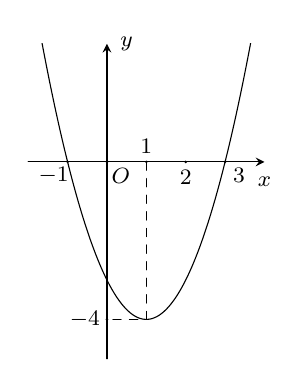
\begin{tikzpicture}[font=\footnotesize,line join=round, line cap=round, >=stealth,scale=0.5] 
\def \xmin{-2}\def \xmax{4}\def \ymin{-5}\def \ymax{3} 
\draw[->] (\xmin,0)--(\xmax,0) node[shift=(-90:0.25)] {$x$};
\draw[->] (0,\ymin)--(0,\ymax) node[shift=(0:0.25)] {$y$};
\fill (0,0) circle(1pt) node[shift=(-45:0.25)]{$O$}
(-1,0) circle(1pt) node[shift=(-135:0.25)]{$-1$}
(2,0) circle(1pt) node[shift=(-90:0.2)]{$2$}
(3,0) circle(1pt) node[shift=(-45:0.25)]{$3$}
(1,0) circle(1pt) node[shift=(90:0.2)]{$1$}
(0,-4) circle(1pt) node[shift=(180:0.28)]{$-4$};
\draw[dashed](1,0)--(1,-4)--(0,-4);
\begin{scope}
\clip (\xmin,\ymin) rectangle (\xmax,\ymax); 
\draw[smooth,samples=100,domain=\xmin:\xmax] plot(\x,{(\x)^2-2*\x-3}); 
\end{scope}
\end{tikzpicture}	
	}
\loigiai{
Dựa vào đồ thị ta có điểm $ (1,-4) \in (P)$, điểm $ (3{,}0) \in (P)$.\\
Suy ra $\heva{&a+b-3=-4\\&9a+3b-3=0}\Leftrightarrow \heva{&a+b=-1\\&3a+b=1}\Leftrightarrow \heva{&a=1\\&b=-2.}$\\
Vậy $ T=2a-b=2\cdot 1-(-2) =4$.
}
\end{bt}

% từ: cau-hoi/lop10/0D3_Ham_so_bac_hai_va_do_thi/0D3-2-1_Xac_dinh_ham_so_bac_hai.tex
\begin{bt}%[0D3V2-1]%[Dự án đề kiểm tra HKI NH22-23-Trương Đăng Khoa]%[THPT Nguyễn Công Trứ]%[ma:e9d52ac6]
	\immini{
		Cho parabol $(P)\colon y=a x^2+b x+c$, ($a \neq 0$) như hình vẽ. Xác định các hệ số $a$, $b$, $c$ của $(P)\colon y=a x^2+b x+c$, ($a \neq 0$).
	}{
		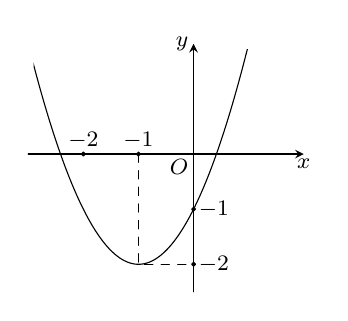
\begin{tikzpicture}[scale=0.7,>=stealth, font=\footnotesize, line join=round, line cap=round]
			\def\a{1} \def\b{2} \def\c{-1} % Hệ số
			\def\xmin{-3} \def\xmax{2}
			\def\ymin{-2.5} \def\ymax{2} 
			%	\draw[color=gray!50,dashed] (\xmin,\ymin) grid (\xmax,\ymax); 
			\draw[->] (\xmin,0)--(\xmax,0) node [below]{$x$};
			\draw[->] (0,\ymin)--(0,\ymax) node [left]{$y$};
			\node at (0,0) [below left]{$O$};
			\clip (\xmin+0.1,\ymin+0.1) rectangle (\xmax-0.5,\ymax-0.1);
			\draw[smooth,samples=300] plot(\x,{\a*(\x)^2+\b*(\x)+\c});
			\draw[dashed] (-1,0)|-(0,-2);
			\draw[fill=black]
			(-1,0)node[above]{$-1$}circle(1pt)
			(-2,0)node[above]{$-2$}circle(1pt)
			(0,-1)node[right]{$-1$}circle(1pt)
			(0,-2)node[right]{$-2$}circle(1pt);
		\end{tikzpicture}
	}
	\loigiai{Đặt $A(0;-1)$, $B(-1;-2)$.\\
		Ta có 
		$\heva{&A(0;-1)\in (P)\colon y=ax^2+bx+c\\ &B(-1;-2)\in (P)\colon y=ax^2+bx+c}\Leftrightarrow \heva{&-1=a\cdot 0^2+b\cdot 0+c\\ & -2=a\cdot (-1)^2+b \cdot (-1)+c}\Leftrightarrow \heva{& c=-1\\ &a-b=-1.\quad (1)}$\\
		Mặt khác đồ thị hàm số nhận đường thẳng $x=-1$ làm trục đối xứng.\\
		Nên $-\dfrac{b}{2a}=-1\Leftrightarrow 2a-b=0$.\quad $(2)$\\
		Từ $(1)$ và $(2)$ ta có hệ $\heva{&a-b=1\\ & 2a-b=0}\Leftrightarrow \heva{&a=1\\ &b=2.}$\\
		Vậy $a=1$, $b=2$, $c=-1$.
	}
\end{bt}

% từ: cau-hoi/lop10/0D3_Ham_so_bac_hai_va_do_thi/0D3-2-2_Bang_bien_thien_tinh_don_dieu_max_min.tex
\begin{bt}%[0D3H2-2]%[Tex hóa SGK CD-CT,T7/22, Nguyễn Tài Tuệ]%[ma:11b82a85]
	\immini{	Tìm tập xác định, giá trị lớn nhất của hàm số, tập giá trị và các khoảng biến thiên của hàm số biết đồ thị hàm số là một parabol có đỉnh $S$ như hình.	}{
		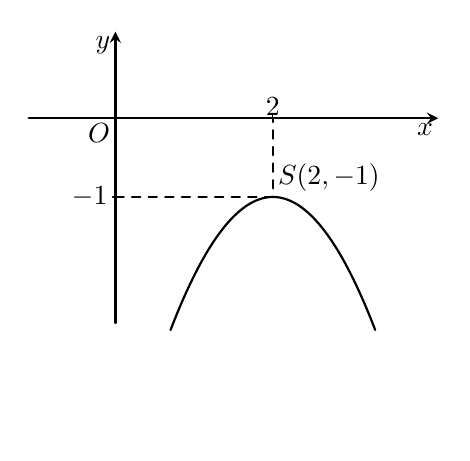
\begin{tikzpicture}[line join=round, line cap=round,>=stealth,thick]
			\tikzset{label style/.style={font=\footnotesize}}
			\draw[->] (-1.1,0)--(4.1,0) node[below left] {$x$};
			\draw[->] (0,-2.6)--(0,1.1) node[below left] {$y$};
			\draw (0,0) node [below left] {$O$};
			\foreach \x in {2}
			\draw[thin] (\x,1pt)--(\x,-1pt) node [above] {$\x$};
			\foreach \y in {-1}
			\draw[thin] (1pt,\y)--(-1pt,\y) node [left] {$\y$};
			\draw[dashed] (0,-1)--(2,-1) node[above right]{$ S(2,-1) $}--(2,0);
			\begin{scope}
				\clip (-1,-4) rectangle (4,1);
				\draw[samples=200,domain=0.7:3.3,smooth,variable=\x] plot (\x,{-1*(\x)^2+4*(\x)+-5});
			\end{scope}
	\end{tikzpicture}}
	\loigiai{
		\begin{itemize}
			\item Hàm số có đồ thị là parabol nên là hàm số bậc hai. Hàm số này có tập xác định $\mathscr{D}=\mathbb{R}$.
			\item Parabol quay bề lõm xuống, có đỉnh $S(2;-1)$ nên hàm số có bảng biến thiên sau 
			\begin{center}
				
\begin{tikzpicture}
					\tkzTabInit[lgt=1.2,espcl=4]
					{$x$/0.8,$f(x)$/2}
					{$-\infty$,$2$,$+\infty$}
					\tkzTabVar{-/$-\infty$,+/$-1$,-/$-\infty$}
				\end{tikzpicture}
			\end{center}
			\item 	Từ đây, ta cũng thấy hàm số có giá trị lớn nhất là $-1$ nên có tập giá trị là $T=(-\infty;-1]$.
		\end{itemize}
	}
\end{bt}

% từ: cau-hoi/lop10/0D3_Ham_so_bac_hai_va_do_thi/0D3-2-3_Do_thi_cua_ham_so_bac_hai.tex
\begin{ex}%[0D3N2-3]%[ma:8067846b]
	\immini[thm]{Cho hàm số bậc hai $y=f(x)$ có đồ thị như  hình vẽ. Tập nghiệm của bất phương trình $f(x)>0$ là
	 \choice
		 {$(0;3)$}
		 {$[-1;3]$}
		 {$(-\infty;-1)\cup(3;+\infty)$}
		 {\True $(-1;3)$}
		}{ 
		\begin{tikzpicture}[line join=round,line cap=round,font=\footnotesize,scale=0.6,>=stealth]
				 \draw[-stealth](-1.5,0)--(4,0) node[above]{$x$};
				 \draw[-stealth](0,-2)--(0,4.5) node[right]{$y$};
				\draw[smooth,samples=100,domain=-1.3:3.3] plot (\x,{-(\x+1)*(\x-3)}); 
				\fill (0,0) circle (1pt) node[below  left]{$O$};
				\foreach \x/\g  in {-1/140,3/50}\fill[black] (\x,0) circle (1pt)+(\g:.4) node{$\x$};
			\end{tikzpicture}
		} 
	 \loigiai{
		Nhìn đồ thị ta thấy phần đồ thị nằm trên trục hoành $f(x)>0$  khi $x\in(-1;3)$.
	 }
\end{ex}

% từ: cau-hoi/lop10/0D3_Ham_so_bac_hai_va_do_thi/0D3-2-6_Toan_thuc_te_ung_dung_ham_so_bac_hai.tex
\begin{bt}%[0D3V2-6] % KIEM_TRA%[ID]%[Dự án đề kiểm tra GKII lớp 10 năm học 2024 - 2025 - Nguyễn Hoàng Anh]%[THPT Sầm Sơn - Tỉnh Thanh Hóa]%[ma:d0403ba4]
	Bác Nam dự định xây dựng một khu vườn hình chữ nhật có chiều dài $10$\,m, trên khu vườn đó bác Nam muốn chia thành hai phần: phần đất trồng rau dạng hình vuông có cạnh bằng với chiều rộng của khu vườn, phần còn lại bác Nam làm hồ nuôi cá. Gọi $x$ ($0<x<10$) là chiều rộng của khu vườn. Biết chi phí thi công phần đất trồng rau và hồ nuôi cá lần lượt là $60\,000$ đồng/m$^2$ và $135\,000$ đồng/m$^2$. Hỏi chiều rộng của khu vườn lớn nhất có thể là bao nhiêu mét để tổng chi phí thi công không vượt quá $5\,400\,000$ đồng.
\begin{center}
	\begin{tikzpicture}[line cap=round,line join=round,font=\footnotesize,scale=1]
		\draw (0,0) rectangle (8,3);
		\draw (3,0)--(3,3);
		\draw[dashed] (0,3) to[out=15,in=165] node[above]{$10$ (m)} (8,3);
		\draw[dashed] (0,0) to[out=-15,in=-165] node[below]{$x$ (m)} (3,0);
		\draw[dashed] (3,0) to[out=-15,in=-165] node[below]{$10-x$ (m)} (8,0);
		\draw[dashed] (0,0) to[out=105,in=255] node[left]{$x$ (m)} (0,3);
	\end{tikzpicture}
\end{center}
	\shortans{$6$}
	\loigiai{\begin{center}
			\begin{tikzpicture}[line cap=round,line join=round,font=\footnotesize,scale=1]
				\draw (0,0) rectangle (8,3);
				\draw (3,0)--(3,3);
				\draw[dashed] (0,3) to[out=15,in=165] node[above]{$10$ (m)} (8,3);
				\draw[dashed] (0,0) to[out=-15,in=-165] node[below]{$x$ (m)} (3,0);
				\draw[dashed] (3,0) to[out=-15,in=-165] node[below]{$10-x$ (m)} (8,0);
				\draw[dashed] (0,0) to[out=105,in=255] node[left]{$x$ (m)} (0,3);
			\end{tikzpicture}
		\end{center}
	Gọi $x$ (m) ($0<x<10$) là chiều rộng của khu vườn.\\
	Do phần đất trồng rau là hình vuông cạnh $x$\,m diện tích của của phần đất trồng rau là $x^2$\,(m$^2$).\\
	Diện tích của hồ nuôi cá là $(10-x)x$ (m$^2$).\\
	Theo giả thiết, ta có bất phương trình
	\begin{eqnarray*}
		&&60\,000x^2+135\,000(10-x)x\leq 5\,400\,000 \\
		&\Leftrightarrow& -75\,000x^2+1\,350\,000x-5\,400\,000\leq 0\\
		&\Leftrightarrow& \hoac{&x\leq 6\\&x\geq 12.}
	\end{eqnarray*}
Kết hợp điều kiện suy ra $0<x\leq 6$.\\
Vậy chiều rộng của khu vườn lớn nhất có thể là $6$ (m).
	}
\end{bt}

% từ: cau-hoi/lop10/0D7_Bat_phuong_trinh_bac_2_mot_an/0D7-2-6_Bai_toan_co_tham_so.tex
\begin{bt}%[0D7V2-6] %[Dự án đề kiểm tra giữa HKII NH22-23- Nguyễn Ngọc Nguyên]%[THPT Bà Điểm]%[ma:decb2335]
	Cho phương trình $(m+3)x^2+2(m+1)x+m+3=0$ ($m$ là tham số). Xác định tất cả các giá trị của $m$ để phương trình đã cho có $2$ nghiệm phân biệt.	
	\loigiai{
 Phương trình đã cho có $2$ nghiệm phân biệt khi và chỉ khi
 \begin{eqnarray*}
 	\heva{&m+3 \ne 0 \\ & \Delta ' >0} \Leftrightarrow \heva{& m \ne -3 \\ & (m+1)^2 -(m+3)^2>0} \Leftrightarrow \heva{&m \ne -3 \\ & -4m-8>0} \Leftrightarrow \heva{&m \ne -3 \\& m<-2.}
 \end{eqnarray*}
Vậy $m \in (-\infty;-2) \setminus \{-3\}$ thỏa yêu cầu bài toán.
	}
\end{bt}

% từ: cau-hoi/lop10/0H4_He_thuc_luong_trong_tam_giac/0H4-1-2_Tinh_cac_gia_tri_luong_giac.tex
\begin{bt}%[0H4V1-2]%[ma:a5beffe9]
% nguon: Archive/2024/TOAN_11_XE/TOAN_11_XE/data4/11C1/KNTT-1.1.tex #1220

	Tính
	\begin{enumerate}
		\item $A=\sin^2 5^\circ+\sin^2 10^\circ+\sin^2 15^\circ+\ldots+\sin^2 85^\circ$ ($17$ số hạng);
		\item $B=\cos 5^\circ+\cos 10^\circ+\cos 15^\circ+\ldots+\cos 175^\circ$ ($35$ số hạng).
	\end{enumerate}
	\loigiai{
		\begin{enumerate}
			\item Nhận xét thấy $\sin^2 85^\circ=\left[\sin (90^\circ-5^\circ)\right]^2=\cos^2 5^\circ$.\\
			Do đó
			\begin{eqnarray*}
				A&=&\sin^2 5^\circ+\sin^2 10^\circ+\sin^2 15^\circ+\ldots+\sin^2 85^\circ\\
				&=&\sin^2 5^\circ+\sin^2 85^\circ+\sin^2 10^\circ+\sin^2 80^\circ+\ldots+\sin^2 45^\circ\\
				&=&\sin^2 5^\circ+\cos^2 5^\circ+\sin^2 10^\circ+\cos^2 10^\circ+\ldots+\sin^2 45^\circ\\
				&=&\underbrace {1+1+\ldots+1}_{8\text{ số hạng}}+\dfrac{1}{2}=\dfrac{17}{2}.
			\end{eqnarray*}
			\item Nhận xét thấy $\cos 175^\circ=\cos (180^\circ-5^\circ)=-\cos 5^\circ$.\\
			Do đó
			\begin{eqnarray*}
				B&=&\cos 5^\circ+\cos 10^\circ+\cos 15^\circ+\ldots+\cos 175^\circ\\
				&=&\cos 5^\circ+\cos 175^\circ+\cos 10^\circ+\cos 170^\circ+\ldots+\cos 90^\circ\\
				&=&\cos 5^\circ-\cos 5^\circ+\cos 10^\circ-\cos10^\circ+\ldots+\cos 90^\circ\\
				&=&\cos 90^\circ\\
				&=&0.
			\end{eqnarray*}
		\end{enumerate}
	}
\end{bt}

% từ: cau-hoi/lop10/0H4_He_thuc_luong_trong_tam_giac/0H4-3-1_Giai_tam_giac.tex
\begin{bt}%[0H4V3-1][Dự án đề kiểm tra HKII NH22-23- Nguyễn Cường]%[THPT Lê Quý Đôn]%[ma:2332e3c5]
	Cho hình thang vuông $ ABCD $ có hai đáy $ AB=a $, $ CD=b $ và chiều cao $ AD=h $. Gọi $ M $ là trung điểm cạnh $ BC $. Biết rằng $ h^2=a^2+ab $. Tính góc giữa $ AM $ và $ BD $.
	\dapso{ $ 90^\circ $}
	\loigiai{\begin{center}
			\begin{tikzpicture}[>=stealth,line join=round,line cap=round,font=\footnotesize,scale=1]
				\path (0,0) coordinate (D)
				(D)++(90:2) coordinate (A)++(0:3)coordinate(B)
				(D)++(0:4) coordinate (C)
				($(B)!.5!(C)$)coordinate(M)
				;
				\draw (B)--(A)node[midway,above]{$a$};
				\draw (A)--(D)node[midway,left]{$h$};
				\draw (D)--(C)node[midway,below]{$b$};
				\draw (D)--(B)--(C) (A)--(M);
				\foreach \p / \r in {A/90,C/0,B/90,D/-90,M/45}
				\fill (\p) circle (1.2pt) node[shift={(\r:3mm)}]{$\p$};
			\end{tikzpicture}
		\end{center}
	Do $M$ là trung điểm $BC$ nên $\overrightarrow{AC}+\overrightarrow{AB}=2\overrightarrow{AM}$.\\
	Khi đó
	\allowdisplaybreaks
	\begin{eqnarray*}
		&&2\overrightarrow{AM}\cdot \overrightarrow{BD}\\
		&=&\left(\overrightarrow{AC}+\overrightarrow{AB}\right)\cdot\left(\overrightarrow{BA}+\overrightarrow{AD}\right)\\
		&=&\left(\overrightarrow{AD}+\overrightarrow{DC}+\overrightarrow{AB}\right)\cdot\left(\overrightarrow{BA}+\overrightarrow{AD}\right)\\
		&=&\overrightarrow{AD}\cdot\overrightarrow{BA}+\overrightarrow{AD}\cdot\overrightarrow{AD}+\overrightarrow{DC}\cdot\overrightarrow{BA}+\overrightarrow{DC}\cdot\overrightarrow{AD}+\overrightarrow{AB}\cdot\overrightarrow{BA}+\overrightarrow{AB}\cdot\overrightarrow{AD}\\
		&=&h^2-ab-a^2\\
		&=&a^2+ab-ab-a^2=0.
	\end{eqnarray*}
Do đó, $AM\perp BD$ hay góc giữa $AM$ và $BD$ là $90^\circ$.
	}
\end{bt}

% từ: cau-hoi/lop10/0H5_Vecto_chua_xet_toa_do/0H5-2-6_Toan_thuc_te_ap_dung_tong_hieu_vecto.tex
\begin{bt}%[0H5V2-6]%[ma:eb232b83]
	\immini{Một dòng sông chảy từ phía bắc xuống phía nam với vận tốc là $10$~$\mathrm{km/h}$. Một chiếc ca nô chuyển động từ phía đông sang phía tây với vận tốc $40$~$\mathrm{km/h}$ so với mặt nước. Tìm vận tốc của ca nô so với bờ sông. (Làm tròn đến chữ số thập phân thứ nhất)}{
			\begin{tikzpicture}[scale=1, font=\footnotesize, line join=round, line cap=round, >=stealth]
				\path 
				(0,0) coordinate (C)
				(0,2) coordinate (B)
				(5,2) coordinate (O)
				(5,0) coordinate (A)
				($(B)!0.5!(O)$) coordinate (M) node[above] {$40$}
				($(A)!0.5!(O)$) coordinate (M) node[right] {$10$}
				;
				\draw[dashed] (B)--(C)--(A);
				\draw[->,thick] (O)--(B);
				\draw[->,thick] (O)--(C);
				\draw[->,thick] (O)--(A);
				\foreach \x/\g in {C/45+180,B/-45+180,O/45,A/-45}
				\fill[black] 	(\x) circle (1pt)
				($(\g:3mm)+(\x)$) node {$\x$};	
			\end{tikzpicture}}
	\shortans[0]{$41{,}2$}
	\loigiai{
		Gọi $O$ là vị trí của ca nô.\\
		Vẽ $\overrightarrow{OA}$ là vận tốc dòng nước (chảy từ phía bắc xuống phía nam), $\overrightarrow{OB}$ là vận tốc riêng của ca nô (chuyển động từ phía đông sang phía tây).\\		
		Khi đó vectơ vận tốc của ca nô so với bờ sông là vectơ $\overrightarrow{OA}+\overrightarrow{OB}$.\\
		Gọi $C$ là đỉnh thứ tư của hình bình hành $OACB$, ta có: $\overrightarrow{OC}=\overrightarrow{OA}+\overrightarrow{OB}$.\\
		Xét tam giác $OBC$ vuông tại $B$ ta có:\\
		$BC=40$; $BC=OA=10$.\\
		$\Rightarrow OC=\sqrt{OB^2+BC^2}=10\sqrt{17}\approx 41{,}2$.}
\end{bt}

% từ: cau-hoi/lop10/0H5_Vecto_chua_xet_toa_do/0H5-2-6_Toan_thuc_te_ap_dung_tong_hieu_vecto.tex
\begin{bt}%[0H5H2-6]%[ma:bc369467]

		Một máy bay có véc-tơ vận tốc chỉ theo hướng bắc, vận tốc gió là một véc-tơ theo hướng đông như hình bên. Tính độ dài véc-tơ tổng của hai véc-tơ nói trên.
		
	\begin{center}
		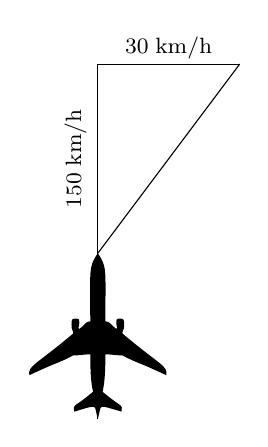
\begin{tikzpicture}[scale=0.6, font=\footnotesize, line join=round, line cap=round, >=stealth]
			\fill[black] (0,0)..controls +(-55:0.35) and +(90:1.1)..(0.16,-1.44)..controls +(0:0.1) and +(145:0.15)..(0.39,-1.6)..controls +(-20:0.03) and +(-40:0.02)..(0.4,-1.54)..controls +(110:0.03) and +(-120:0.02)..(0.4,-1.4)..controls +(70:0.03) and +(100:0.02)..(0.54,-1.4)..controls +(-40:0.03) and +(40:0.03)..(0.54,-1.62)..controls +(-120:0.1) and +(140:0.02)..(0.56,-1.73)..controls +(-40:1) and +(80:0.2)..(1.45,-2.58)..controls +(155:0.8) and +(-28:0.4)..(0.52,-2.16)..controls +(180:0.2) and +(0:0.2)..(0.16,-2.14)..controls +(-90:0.3) and +(75.6:0.2)..(0.1,-2.93)..controls +(-40:0.6) and +(85.6:0.18)..(0.5,-3.35)..controls +(164:0.57) and +(72.6:0.32)..(0.,-3.5)--cycle;
			\fill[black,xscale=-1] (0,0)..controls +(-55:0.35) and +(90:1.1)..(0.16,-1.44)..controls +(0:0.1) and +(145:0.15)..(0.39,-1.6)..controls +(-20:0.03) and +(-40:0.02)..(0.4,-1.54)..controls +(110:0.03) and +(-120:0.02)..(0.4,-1.4)..controls +(70:0.03) and +(100:0.02)..(0.54,-1.4)..controls +(-40:0.03) and +(40:0.03)..(0.54,-1.62)..controls +(-120:0.1) and +(140:0.02)..(0.56,-1.73)..controls +(-40:1) and +(80:0.2)..(1.45,-2.58)..controls +(155:0.8) and +(-28:0.4)..(0.52,-2.16)..controls +(180:0.2) and +(0:0.2)..(0.16,-2.14)..controls +(-90:0.3) and +(75.6:0.2)..(0.1,-2.93)..controls +(-40:0.6) and +(85.6:0.18)..(0.5,-3.35)..controls +(164:0.57) and +(72.6:0.32)..(0.,-3.5)--cycle;
			\draw[black] (0,0)--(0.,-3.5);
			\draw(0,0)--(0,4);
			\draw(0,4)--(3,4);
			\draw(0,0)--(3,4);
			\node[rotate=90,yshift=8] at (0,2){$150\mathrm{\;km/h}$};
			\node[above] at (1.5,4){$30\mathrm{\;km/h}$};
	\end{tikzpicture}\end{center}
	
	\shortans[3]{$153$}	
		\loigiai{
			Gọi $\overrightarrow{v}$ là véc-tơ vận tốc của máy bay và $\overrightarrow{g}$ là véc-tơ vận tốc gió.\\
			Theo giả thiết, ta có: $\left|\overrightarrow{v}\right|=150\mathrm{\;km/h}$ và $\left|\overrightarrow{g}\right|=30\mathrm{\;km/h}$.\\
			Do giá của $\overrightarrow{v}$ và $\overrightarrow{g}$ vuông góc nhau nên $\left|\overrightarrow{v}+\overrightarrow{g}\right|$ là cạnh huyền của tam giác vuông có hai cạnh góc vuông là $150$ và $30$.\\
			Do đó $\left|\overrightarrow{v}+\overrightarrow{g}\right|=\sqrt{150^2+30^2}=30\sqrt{26}\approx 153\mathrm{\;km/h}$.
		}

\end{bt}

% từ: cau-hoi/lop10/0H9_Phuong_phap_toa_do_trong_mat_phang/0H9-3-2_Phuong_trinh_duong_thang.tex
\begin{bt}%[0H9H3-2]%[1,0 điểm]%[ma:c758b06e]
	Trong mặt phẳng $Oxy$, cho tam giác $ABC$ với $A(2; 6)$, $B(-3;-4)$ và $C(5; 1)$.
	\begin{enumerate}[a)]
		\item Viết phương trình tổng quát đường cao $AH$ của tam giác $ABC$.
		\item Tìm tọa độ tâm đường tròn ngoại tiếp $\triangle ABC$.
	\end{enumerate}
	\loigiai{
		\begin{enumerate}[a)]
			\item Viết phương trình tổng quát đường cao $AH$ của tam giác $ABC$.\\
				Đường cao $AH$ nhận véc-tơ $\overrightarrow{BC}=(8;5)$ là véc-tơ pháp tuyến.\\
				Phương trình của $AH\colon 8x+5y-46=0$.
			\item Tìm tọa độ tâm đường tròn ngoại tiếp $\triangle ABC$.\\
				Gọi phương trình đường tròn ngoại tiếp $\triangle ABC$ là $x^2+y^2+2ax+2by+c=0$.\\
				Đường tròn đi qua $3$ điểm $A$, $B$, $C$ suy ra
				\[\heva{&-4a-12b+c=-40\\&6a+8b+c=-25\\&-10a-2b+c=-26} \Leftrightarrow \heva{&a=-\dfrac{13}{22}\\&b=\dfrac{23}{22}\\&c=-\dfrac{328}{11}.}\]
				Vậy tọa độ tâm đường tròn ngoại tiếp $\triangle ABC$ là $I\left(-\dfrac{13}{22}; \dfrac{23}{22}\right)$.
		\end{enumerate}
	}
\end{bt}

% từ: cau-hoi/lop10/0H9_Phuong_phap_toa_do_trong_mat_phang/0H9-3-7_Bai_toan_dung_cho_tam_giac_tu_giac.tex
\begin{bt}%[0H9V3-7]%[Dự án đề kiểm tra HKII NH22-23-Nguyễn Tài Tuệ]%[THPT Chuyên Lê QUý Đôn- Quảng Trị]%[ma:9abdd75d]
	  Trong mặt phẳng tọa độ $Oxy$, cho hình chữ nhật $ABCD$. Kẻ $BH \perp AC ~(H \in AC)$. Gọi $M$, $N$ lần lượt là trung điểm của $AH$ và $DC$. Biết $M(11; 12)$, $N(10 ; 5)$, $H(17 ; 4)$.
	  \begin{enumerate}
	  	\item Tìm tọa độ điểm $A$ và tính diện tích tam giác $HMN$.
	  	\item  Tìm tọa độ điểm $B$.
	  \end{enumerate}
	 \loigiai{
	 	\begin{center}
	 	
	  \begin{tikzpicture}
	  	\path
	  	(0,0)  coordinate (D)
	  	(4,0) coordinate (C)
	  	(4,3) coordinate (B)
	  	(0,3) coordinate (A)
	  	($ (A)!(B)!(C)$) coordinate (H)
	  	($ (A)!0.5!(H) $) coordinate (M)
	  	($ (D)!0.5!(C) $) coordinate (N)
	  	;
	  	\draw (A)--(B)--(C)--(D)--cycle (A)--(C) (H)--(B)--(M)--(N) --(H);
	  	\foreach \p/\g in {A/90,B/90,C/-90,D/-90,M/-150,N/-90,H/100} \draw[fill] (\p) circle(.5pt)node [shift={(\g:.3)}] {$\p$};
	  \end{tikzpicture}  	 
\end{center}
 
	 	\begin{enumerate}
	 		\item Ta có $\overrightarrow{M A}\left(x_A-11 ; y_A-12\right)=\overrightarrow{H M}(-6 ; 8) \Rightarrow A(5 ; 20)$.\\
	 		Suy ra    $MN=\sqrt{(10-11)^2+(5-12)^2}=\sqrt{50}$, $NH=\sqrt{(17-10)^2+(4-5)^2}=\sqrt{50}$, $MH=\sqrt{(17-11)^2+(4-12)^2}=10$. \\
	 		Sử dụng công thức Hê-rông, diện tích tam giác $ HMN $  ta có \\
	 		 $ S=\sqrt{p\cdot (p-MN)(p-MH)(p-HN)}=25 $, với $ p=\dfrac{MN+NH+HN}{2}. $  
	 		\item Ta có 
	 		\begin{eqnarray*}
	 			 \overrightarrow{B M} \cdot \overrightarrow{M N}
	 			 &=&\dfrac{1}{2}\left (\overrightarrow{B A}+\overrightarrow{B H}\right )\left (\overrightarrow{M C}+\overrightarrow{C N}\right  )=\dfrac{1}{2}\left (\overrightarrow{B A} \cdot \overrightarrow{M C}+\overrightarrow{B A} \cdot \overrightarrow{C N}+\overrightarrow{B H} \cdot \overrightarrow{C N}\right ) \\ & =&\dfrac{1}{2}\left(\overrightarrow{B A} \cdot \overrightarrow{M C}+\dfrac{1}{2} \overrightarrow{B A} \cdot \overrightarrow{B A}+\dfrac{1}{2} \overrightarrow{B H} \cdot \overrightarrow{B A}\right)=\dfrac{1}{2} \overrightarrow{B A}\left (\overrightarrow{M C}+\overrightarrow{B M}\right )\\
	 			 &=&\dfrac{1}{2} \overrightarrow{B A} \cdot \overrightarrow{B C}=0.
	 		\end{eqnarray*}
 		 Gọi $B(a ; b)$. Ta có 
 		 $$
 		\heva{& \overrightarrow{ H B } \cdot \overrightarrow{ M H } = 0   \\
 		 	& \overrightarrow{ M B } \cdot \overrightarrow{ M N } = 0 }
 		\Leftrightarrow \heva{
 		 	 & 6 ( a - 1 7 ) - 8 ( b - 4 ) = 0   \\
 		 	& - ( a - 1 1 ) - 7 ( b - 1 2 ) = 0  
 	} \Leftrightarrow \heva{
 		 	&a=25 \\
 		 &	b=10.} $$
 		 Vậy $B(25 ; 10)$.
	 		 
	 	\end{enumerate}
	 }
\end{bt}

% từ: cau-hoi/lop10/0H9_Phuong_phap_toa_do_trong_mat_phang/0H9-3-8_Bai_toan_thuc_te_PP_toa_do_hoa.tex
\begin{bt}%[0H9V3-8]%[ma:77b6f2f3]
	Đường thẳng $\Delta$ ở hình bên dưới biểu thị tổng chi phí lắp đặt và tiền cước sử dụng dịch vụ Internet (đơn vị: trăm nghìn đồng) theo thời gian của một gia đình (đơn vị: tháng).\\
	\begin{enumerate}
		\item Viết phương trình của đường thẳng $\Delta$.
		\item Cho biết giao điểm của đường thẳng $\Delta$ với trục tung trong tình huống này có ý nghĩa gì.
		\item Tính tổng chi phí lắp đặt và sử dụng Internet trong $12$ tháng đầu tiên.
	\end{enumerate}
	\begin{center}
		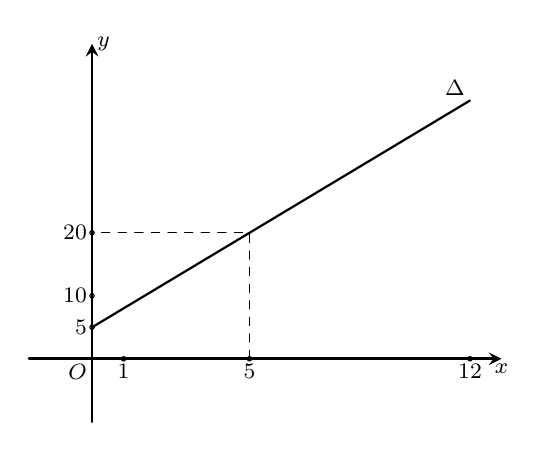
\begin{tikzpicture}[scale=0.8, font=\footnotesize, line join=round, line cap=round, >=stealth]
			\draw[->,line width = 1pt] (-1,0)--(0,0) node[below left]{$O$}--(6.5,0) node[below]{$x$};
			\draw[->,line width =1 pt] (0,-1)--(0,5) node[right]{$y$};
			\draw [thick,domain=0:6,samples=100] 
			plot (\x,{(3/5)*(\x)+1/2}) node [above left] {$\Delta$};
			\draw (0,0.5) node [left] {$5$} circle (1pt);
			\draw (0,1) node [left] {$10$} circle (1pt);		
			\draw (0,2) node [left] {$20$} circle (1pt);
			\draw (0.5,0) node [below] {$1$} circle (1pt);
			\draw (2.5,0) node [below] {$5$} circle (1pt);
			\draw (6,0) node [below] {$12$} circle (1pt);
			\draw [dashed] (2.5,0)--(2.5,2)--(0,2);
		\end{tikzpicture}	
	\end{center}
	\loigiai{
		\begin{enumerate}
			\item Đường thẳng $\Delta$ đi qua hai điểm lần lượt có tọa độ $(0;\,5)$ và $(5;\,20)$ nên $\Delta$ có phương trình là
			$$\dfrac{x-0}{5-0}=\dfrac{y-5}{20-5}\Leftrightarrow\dfrac{x}{5}=\dfrac{y-5}{15}\Leftrightarrow\dfrac{x}{1}=\dfrac{y-5}{3}\Leftrightarrow3x-y+5=0\Leftrightarrow y=3x+5.$$
			\item Giao điểm của đường thẳng $\Delta$ với trục $Oy$ ứng với $x=0$. Thời điểm $x=0$ cho biết mức phí ban đầu lắp đặt để sử dụng Internet. Khi $x=0$ thì $y=5$, vì vậy chi phí lắp đặt ban đầu là $500000$ đồng.
			\item $12$ tháng đầu tiên ứng với $x=12$. Do đó $y=3\cdot12+5=41$.\\
			Vậy tổng chi phí lắp đặt và sử dụng Internet trong $12$ tháng đầu tiên là $4100000$ đồng.
		\end{enumerate}
		
	}
\end{bt}

% từ: cau-hoi/lop10/0H9_Phuong_phap_toa_do_trong_mat_phang/0H9-4-7_Bai_toan_thuc_te_PP_toa_do_hoa.tex
\begin{bt}%[0H9V4-7]%[Dự án đề kiểm tra GHKII NH22-23- Hiếu Mai]%Câu 9%[ma:e5adbe24]
\immini [thm]{Trong mặt phẳng $Oxy$, một vật chuyển động tròn đều ngược chiều kim đồng hồ trên đường tròn tâm	$I(2;2)$ bán kính $R=5$. Dưới tác dụng của lực căng tác dụng lên sợi dây $IM$. Khi vật chuyển động tới điểm $M(5; 6)$ thì dây căng bị đứt (tham khảo hình vẽ). Viết phương trình quỹ đạo $Mt$ chuyển động của vật sau khi dây bị đứt (biết vật chỉ chịu tác động duy nhất lực căng dây).
}
{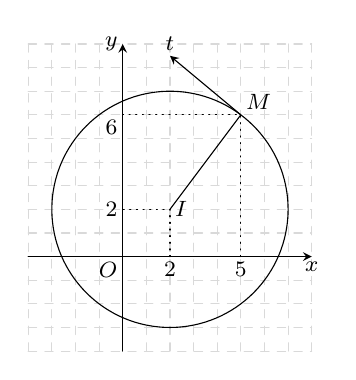
\begin{tikzpicture}[scale=0.3,>=stealth, font=\footnotesize, line join=round, line cap=round]
		\def\a{1} \def\b{-4} \def\c{3} % Hệ số
		\def\xmin{-4} \def\xmax{8}
		\def\ymin{-4} \def\ymax{9}
		\draw[color=gray!30,dashed] (\xmin,\ymin) grid (\xmax,\ymax);	
		\draw[->] (\xmin,0)--(\xmax,0) node [below]{$x$};
		\draw[->] (0,\ymin)--(0,\ymax) node [left]{$y$};
		\node at (0,0) [below left]{$O$};
%		\clip (\xmin+0.1,\ymin+0.1) rectangle (\xmax-0.1,\ymax-0.1);
		\draw (2,2) circle (5 cm) node[right] {$I$} (2,2)--(5,6);
		\draw[->] (5,6) node [above right]{$M$}--++(-3,2.5) node [above]{$t$};
		\draw[dotted] (5,0) node[below] {$5$}|-(0,6)node[below left] {$6$}  (2,0)node[below] {$2$}|-(0,2)node[left] {$2$};
	\end{tikzpicture}
}
	\loigiai{
Ta có $\overrightarrow{IM}=(3;4)$.\\
Theo đề bài, quỹ đạo chuyển động của vật là tia $Mt$ nằm trên tiếp tuyến tại $M$ của đường tròn (theo phương có hoành độ âm).\\
Tia $Mt$ có một véc-tơ chỉ phương là $\overrightarrow{u}=(-4;3)$.\\
Phương trình quỹ đạo $Mt$ là $\heva{&x=5-4t\\&y=6+3t}$ với $t>0$.	
	}
\end{bt}

% từ: cau-hoi/lop10/0H9_Phuong_phap_toa_do_trong_mat_phang/0H9-4-7_Bai_toan_thuc_te_PP_toa_do_hoa.tex
\begin{bt}%[0H9V4-7]%[Dự án đề kiểm tra HKII NH22-23- Lê Hùng Thắng]%[THPT Nguyễn Thượng Hiền]%Câu 8%[ma:30667d3b]
\immini [thm]{Hình bên dưới mô phỏng một trạm thu phát sóng điện thoại di động đặt ở vị trí $I$ có toạ độ $(-2;1)$ trong mặt phẳng toạ độ (đơn vị trên hai trục là ki-lô-mét).
\begin{listEX}[1]
	\item Lập phương trình đường tròn mô tả ranh giới bên ngoài của vùng phủ sóng, biết rằng trạm thu phát sóng đó được thiết kế với bán kính phủ sóng $3$ km.
	\item Tính theo đường chim bay, xác định khoảng cách ngắn nhất để một người ở vị trí $B$ có toạ độ $(-3;4)$ di chuyển được tới vùng phủ sóng theo đơn vị ki-lô-mét.
\end{listEX}
}
{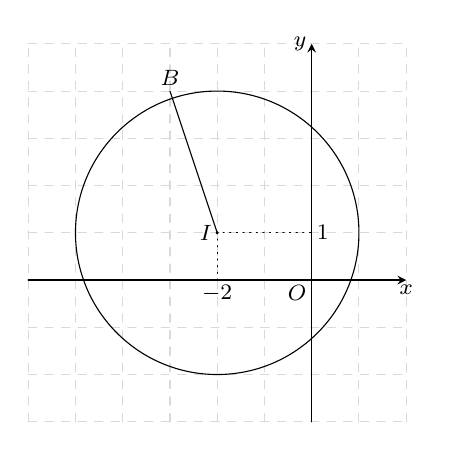
\begin{tikzpicture}[scale=0.6,>=stealth, font=\footnotesize, line join=round, line cap=round]
		\def\xmin{-6} \def\xmax{2}
		\def\ymin{-3} \def\ymax{5}
		\draw[color=gray!30,dashed] (\xmin,\ymin) grid (\xmax,\ymax);
		\draw[->] (\xmin,0)--(\xmax,0) node [below]{$x$};
		\draw[->] (0,\ymin)--(0,\ymax) node [left]{$y$};
		\node at (0,0) [below left]{$O$};
		\clip (\xmin+0.1,\ymin+0.1) rectangle (\xmax-0.1,\ymax-0.1);
		\draw (-2,1)node [left] {$I$} circle (3) (-3,4)node [above] {$B$}--(-2,1);
		\draw[dotted](-2,0) node [below] {$-2$}|-(0,1) node [right]{$1$};
		\fill (-2,1) circle (1pt) 
		(-2,1) circle (1pt);
	\end{tikzpicture}
}
	\loigiai{
	\begin{listEX}[1]
	\item Đường tròn mô tả ranh giới có tâm là $I(-2;1)$ và có bán kính $R=3$ nên phương trình của đường tròn là $(x+2)^2+(y-1)^2=9$.
	\item Ta có $\overrightarrow{BI}=(1;-3) \Rightarrow BI=\sqrt{10}>3=R$.\\
	Từ vị trí $B$ để đường đi đến vùng phủ sóng ngắn nhất thì phải đi theo hướng $\overrightarrow{BI}$.\\
	Quãng đường đi ngắn nhất là $d=BI-R=\sqrt{10}-3 \approx 0{,}162$ km.	
	\end{listEX}	
	}
\end{bt}

% từ: cau-hoi/lop10/0H9_Phuong_phap_toa_do_trong_mat_phang/0H9-4-7_Bai_toan_thuc_te_PP_toa_do_hoa.tex
\begin{bt}%[0H9V4-7]%[Làm đề GHK, HK, 4 phần - 2025]%[Huỳnh Xuân Tín]%[ma:c9577a0e]
	\immini[thm]{Hình mô phỏng một trạm thu phát sóng điện thoại di động đặt ở vị trí $I$ có tọa độ $(-2;1)$ trong mặt phẳng toạ độ (đơn vị trên hai trục là ki-lô-mét). Bán kính phủ sóng là $3$ km. Tính theo đường chim bay, xác định khoảng cách ngắn nhất để một người ở vị trí có tọa độ $(-3;4)$ di chuyển được tới vùng phủ sóng theo đơn vị ki-lô-mét (làm tròn kết quả đến hàng phần mười).
	}{
		\begin{tikzpicture}[line join=round,font=\footnotesize,scale=.6,>=stealth]
			\path (0,0) coordinate (O) (-3,4) coordinate (M) (-2,1) coordinate (I) 
			node[shift={(120:1.2)},text width=2cm,align=center]{\scriptsize Trạm phát sóng};
			\draw[-stealth] (-5.5,0)--(2.5,0) node[below] {$x$};
			\draw[-stealth] (0,-2)--(0,4.5) node[left] {$y$};
			\draw (I) circle (3);
			\draw[dashed] (-2,0)node[below]{$-2$}|-(0,1) node[right]{$1$};
			\foreach \i/\j in {I/135,O/-135,M/90}
			\fill (\i) circle (1.3pt) node[shift={(\j:3mm)}]{$\i$};
		\end{tikzpicture}\vspace{2mm}
	}
	\shortans[]{$0{,}2$}
	\loigiai{
		Ta có $IM=\sqrt{(-3+2)^2+(4-1)^2}=\sqrt{10}$ km.\\
		Vì $IM>R$ nên $M$ đang ở ngoài vùng phủ sóng.\\
		Do đó người ở vị trí $M$ cần di chuyển ít nhất một khoảng bằng $IM-R=\sqrt{10}-3 \approx 0{,}2$ km.
	}
\end{bt}

% từ: cau-hoi/lop10/0H9_Phuong_phap_toa_do_trong_mat_phang/0H9-5-0_Bai_toan_tong_hop_thuc_te_PP_toa_do_hoa_3_duo.tex
\begin{bt}%[0H9V5-0]%[ma:75cc0312]
	\immini
	{Điều hướng LORRAN (điều hướng vô tuyến đường dài) cho máy bay và tàu thủy sử dụng các xung đồng bộ được truyền bởi hai trạm phát đặt cách xa nhau. Các xung này di chuyển với tốc độ ánh sáng ($186\,000$ dặm/giây). Sự chênh lệch về thời gian nhận được phản xạ của các xung này từ một máy bay hoặc tàu thủy là không đổi, nên máy bay hoặc con tàu sẽ nằm trên một hyperbol có các trạm phát là các tiêu điểm.	
	}
	{\begin{tikzpicture}[>=stealth,scale=.45, line join=round, line cap=round,font=\scriptsize]
			\draw[->] (-8,0)--(0.25,0)node[below left]{$ O $}--(8,0) node [below]{$x$};
			\draw[->] (0,-5.5)--(0,6) node [left]{$y$};
			%Hypebol
			\draw[fill=blue] (5.65,3)--(6.8,2.8)--(6.0,4.5)--cycle;
			\clip (-8,-5) rectangle (8,5);
			\draw[orange,thick,smooth,samples=100,domain=4:8] plot(\x,{3*sqrt(\x*\x/16-1)});
			\draw[orange,thick,smooth,samples=100,domain=-4:-8] plot(\x,{3*sqrt(\x*\x/16-1)});
			\draw[orange,thick,smooth,samples=100,domain=4:8] plot(\x,{-3*sqrt(\x*\x/16-1)});
			\draw[orange,thick,smooth,samples=100,domain=-4:-8] plot(\x,{-3*sqrt(\x*\x/16-1)});
			%Đỉnh
			\draw [fill=black]  (-2.25,0)node[below]{$ -50 $} (-6.75,0)node[above]{Trạm 2}circle(1.5pt) (6.75,0)node[above]{ Trạm 1 }circle(1.5pt) (5.65,3)circle(1.5pt)  (-6.75,0)node[below]{$ -150 $} (2.25,0)node[below]{$ 50 $}  (6.75,0)node[below]{$ 150 $} (0,4.5)node[left]{$ 100 $} (0,2.25)node[left]{$ 50 $} (0,-2.25)node[left]{$ -50 $} ;
			\draw (-6.75,-0.2)--(-6.75,0.2) (-4.5,-0.2)--(-4.5,0.2) (-2.25,-0.2)--(-2.25,0.2)
			(2.25,-0.2)--(2.25,0.2) (4.5,-0.2)--(4.5,0.2) (6.75,-0.2)--(6.75,0.2)
			(-0.2,2.25)--(0.2,2.25) (-0.2,4.5)--(0.2,4.5) (-0.2,-2.25)--(0.2,-2.25)
			;
			\fill[teal] (5,0)--(5.1,-0.2)--(4.8,-0.5)--(4.9,-1)--(5.2,-1.1)--(5.3,-1.2)--(5.5,-0.5)--(5.4,0)--cycle (5.3,-1.2)--(6,-2)node[below right]{Bay}
			;
			\draw[dashed,red] (-6.75,0)--(5.65,3)--(6.75,0) ;
	\end{tikzpicture}	
	}\noindent
	Giả sử rằng hai trạm phát, cách nhau $300$ dặm, được đặt trên một hệ tọa độ vuông góc tại các điểm có tọa độ $\left(-150;0\right)$ và $\left(150;0\right)$ và một con tàu đang đi trên một con đường là một nhánh của hypebol và có tọa độ $(x;75)$ (xem hình vẽ). Tính gần đúng hoành độ của vị trí con tàu khi chênh lệch thời gian giữa các xung từ các trạm phát là 1000 micro giây (0,001 giây). Kết quả làm tròn đến hàng đơn vị.
	\shortans[]{$110$}
	\loigiai{
		\immini
		{Gọi đường đi của con tàu là $(H)$ thì $(H)$ có phương trình dạng $\dfrac{x^2}{a^2}-\dfrac{y^2}{b^2}=1$.\\
			Với giả thiết ta có các tiêu điểm của $(H)$ là $F_1\left(-150;0\right)$, $F_2\left(150;0\right)$, suy ra $c=150$.\\
			Giả sử vị trí con tàu hiện tại là $M\left(x;75\right)\in(H)$.
		}
		{\begin{tikzpicture}[>=stealth,scale=.35, line join=round, line cap=round,font=\scriptsize]
				\draw[->] (-8,0)--(0.25,0)node[below left]{$ O $}--(8,0) node [below right]{$x$};
				\draw[->] (0,-5.5)--(0,6) node [left]{$y$};
				%Hypebol
				\draw[fill=blue] (5.65,3)--(6.8,2.8)--(6.0,4.5)--cycle;
				\clip (-9,-5) rectangle (9,5);
				\draw[orange,thick,smooth,samples=100,domain=4:8] plot(\x,{3*sqrt(\x*\x/16-1)});
				\draw[orange,thick,smooth,samples=100,domain=-4:-8] plot(\x,{3*sqrt(\x*\x/16-1)});
				\draw[orange,thick,smooth,samples=100,domain=4:8] plot(\x,{-3*sqrt(\x*\x/16-1)});
				\draw[orange,thick,smooth,samples=100,domain=-4:-8] plot(\x,{-3*sqrt(\x*\x/16-1)});
				%Đỉnh
				\draw [fill=black]  (-2.25,0)node[below]{$ -50 $} (-6.75,0)node[above]{Trạm 2}circle(1.5pt) (6.75,0)node[above]{ Trạm 1 }circle(0.2cm) (5.65,3)node[above left]{ $M$ }circle(0.2cm)  (6.75,0)node[below left]{ $F_2$ }circle(0.2cm)
				(-6.75,0)node[below right]{ $F_1$ }circle(0.2cm) (-6.75,0)node[below left]{$ -150 $} (2.25,0)node[below]{$ 50 $}  (6.75,0)node[below right]{$ 150 $} (0,4.5)node[left]{$ 100 $} (0,2.25)node[left]{$ 50 $} (0,-2.25)node[left]{$ -50 $} ;
				\draw (-6.75,-0.2)--(-6.75,0.2) (-4.5,-0.2)--(-4.5,0.2) (-2.25,-0.2)--(-2.25,0.2)
				(2.25,-0.2)--(2.25,0.2) (4.5,-0.2)--(4.5,0.2) (6.75,-0.2)--(6.75,0.2)
				(-0.2,2.25)--(0.2,2.25) (-0.2,4.5)--(0.2,4.5) (-0.2,-2.25)--(0.2,-2.25)
				;
				\fill[teal] (5,0)--(5.1,-0.2)--(4.8,-0.5)--(4.9,-1)--(5.2,-1.1)--(5.3,-1.2)--(5.5,-0.5)--(5.4,0)--cycle (5.3,-1.2)--(6,-2)node[below right]{Bay}
				;
				\draw[dashed,red] (-6.75,0)--(5.65,3)--(6.75,0) ;
		\end{tikzpicture}	
		}\noindent
		Theo giả thiết độ chênh lệch thời gian giữa các xung từ các trạm phát là $1\,000$ micro giây ($0{,}001$ giây), tức là ta có $\left| M{F_1}-M{F_2}\right|=0{,}001\cdot 186\,000=186$ (dặm);\\
		Khi đó $2a=186\Rightarrow a=93$.\\
		Suy ra $b=\sqrt{c^2-a^2}=27\sqrt{19}$.\\
		Phương trình $(H)\colon \dfrac{x^2}{8649}-\dfrac{y^2}{13851}=1$.\\
		Ta có $M\left(x;75\right) \in(H) \Leftrightarrow \dfrac{x^2}{8649}-\dfrac{75^2}{13851}=1 \Leftrightarrow \hoac{& x\approx 110{,}2789\\ & x\approx-110{,}2789.}$\\
		Vậy hoành độ của con tàu gần bằng $110{,}2789$.\\
		Kết quả làm tròn đến hàng đơn vị là $110$.
		}
\end{bt}

% từ: cau-hoi/lop10/0H9_Phuong_phap_toa_do_trong_mat_phang/0H9-5-0_Bai_toan_tong_hop_thuc_te_PP_toa_do_hoa_3_duo.tex
\begin{bt}%[0H9V5-0]%[ma:9bfb2ab7]
	Một cột trụ hình hypebol (H.7.36), có chiều cao $6$ m, chỗ nhỏ nhất ở chính giữa và rộng $0{,}8$ m, đỉnh cột và đáy cột đều rộng $1$ m. Tính độ rộng của cột ở độ cao $5$ m (tính theo đơn vị mét và làm tròn tới hai chữ số sau dấu phầy).
\begin{center}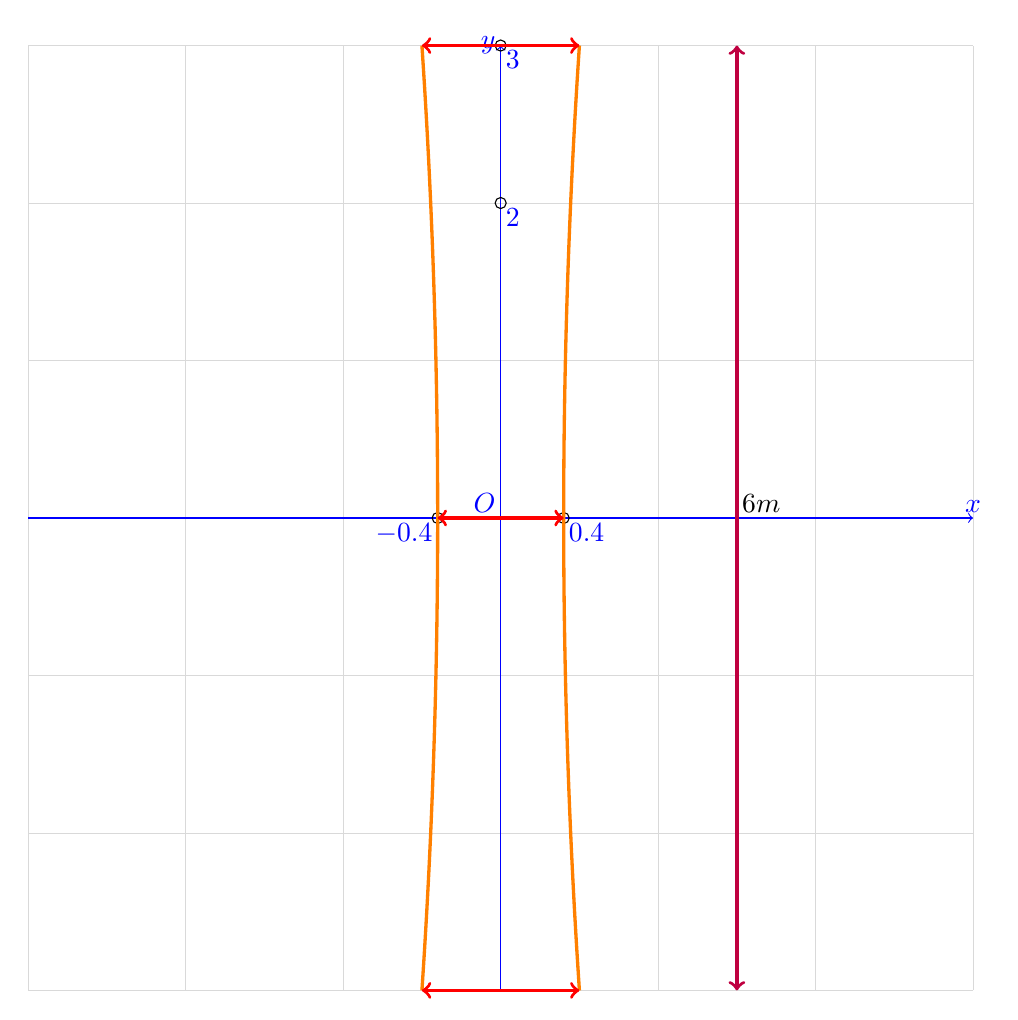
\begin{tikzpicture}[scale=2]
		\draw[step=1,gray, very thin,opacity=0.3](-3,-3) grid (3,3);
		\draw [->,blue] (-3,0) -- (3,0) node[above] {$x$};
		\draw [->,blue] (0,-3) -- (0,3) node[left] {$y$};
		\draw (-0.4,0) node[below left,blue]{$-0.4$} circle (1pt);
		\draw (0.4,0) node[below right,blue]{$0.4$} circle (1pt);
		\foreach \y in {2,3} {\draw (0,\y) node[below right,blue] {$\y$} circle (1pt);}
		\draw (0,0) node [above left,blue]{$O$};
		\draw[smooth,orange, very thick] plot[domain=-3:3] ({(1/90)*(\x)^2+(2/5)}, \x);
		\draw[smooth,orange, very thick] plot[domain=-3:3] ({(-1/90)*(\x)^2-(2/5)}, \x);
		\draw[<->,red,very thick] (-0.4,0) -- (0.4,0);
		\draw[<->,red,very thick] (-0.5,3) -- (0.5,3);
		\draw[<->,red,very thick] (-0.5,-3) -- (0.5,-3);
		\draw[<->,purple,very thick] (1.5,-3) -- (1.5,3);
		\draw (1.5,0) node[above right] {$6 \text{m}$};
\end{tikzpicture}\end{center}
	\shortans{$1{,}28$}
	\loigiai{
		Gắn hệ trục tọa độ $Oxy$ vào cột trụ hình Hypebol đã cho như hình trên.\\
		Tiếp theo ta tìm phương trình của cột trụ hình Hypebol này.\\
		Gọi phương trình của cột trụ là
		$$\dfrac{x^{2}}{a^{2}}-\dfrac{y^{2}}{b^{2}}=1$$
		Vì $Oy$ là đường trung trực của đoạn thẳng $0,8$ m nên $Oy$ chia đoạn thẳng $0,8$ m thành hai đoạn bằng nhau, mỗi đoạn $0,4$ m, tức Hypebol đi qua hai điểm $A_1(-0,4;0), A_2(0,4;0)$.\\
		Khi đó ta có 
		$$\dfrac{{0{,}4}^{2}}{a^{2}}-\dfrac{0^{2}}{b^{2}}=1$$
		$$\Leftrightarrow \dfrac{{0{,}4}^{2}}{a^{2}}=1$$
		$$\Leftrightarrow a=0{,}4.$$
		(vì $a>0$)\\
		Lúc này ta được phương trình Hypebol: $$\dfrac{x^{2}}{0{,}16}-\dfrac{y^{2}}{b^{2}}=1$$
		Vì $Oy$ là đường trung trực của đoạn thẳng $1$ m nên $Oy$ chia đoạn thẳng $1$ m thành hai đoạn bằng nhau, mỗi đoạn $0,5$ m, tức Hypebol đi qua hai điểm $B_1(-0,5;3), B_2(0,5;3)$.\\
		Khi đó ta có
		$$\dfrac{{0{,}5}^{2}}{0{,}16}-\dfrac{3^{2}}{b^{2}}=1$$
		$$\Leftrightarrow \dfrac{3^{2}}{b^{2}}=\dfrac{9}{16}$$
		$$\Leftrightarrow b=4.$$
		(vì $b>0$)\\
		Vậy ta đã tìm được phương trình Hypebol của cột trụ:
		$$\dfrac{x^{2}}{0{,}16}-\dfrac{y^{2}}{16}=1$$
		Khi cột trụ ở độ cao $5$ m thì
		$$\dfrac{x^{2}}{0{,}16}-\dfrac{5^{2}}{16}=1$$
		$$\Leftrightarrow \dfrac{x^{2}}{0{,}16}=\dfrac{41}{16}$$
		$$\Leftrightarrow x^{2}=\dfrac{41}{100}$$
		$$\Leftrightarrow |x|=\dfrac{\sqrt{41}}{10}$$
		Vậy độ rộng của cột ở độ cao $5$ m là $2.|x|=2.\dfrac{\sqrt{41}}{10}=\dfrac{\sqrt{41}}{5} \approx 1{,}28 \;$ m.
	}
\end{bt}

% từ: cau-hoi/lop10/0H9_Phuong_phap_toa_do_trong_mat_phang/0H9-5-0_Bai_toan_tong_hop_thuc_te_PP_toa_do_hoa_3_duo.tex
\begin{bt}%[0H9V5-0]%[ma:edfac2e5]
	Điều hướng LORRAN (điều hướng vô tuyến đường dài) cho máy bay và tàu thủy sử dụng các xung đồng bộ được truyền bởi hai trạm phát đặt cách xa nhau. Các xung này di chuyển với tốc độ ánh sáng ($186\,000$ dặm/giây). Sự chênh lệch về thời gian nhận được phản xạ của các xung này từ một máy bay hoặc tàu thủy là không đổi, nên máy bay hoặc con tàu sẽ nằm trên một hyperbol có các trạm phát là các tiêu điểm. Giả sử rằng hai trạm phát, cách nhau $300$ dặm, được đặt trên một hệ tọa độ vuông góc tại các điểm có tọa độ $\left(-150;0\right)$ và $\left(150;0\right)$ và một con tàu đang đi trên một con đường là một nhánh của hypebol và có tọa độ $(x;75)$ (xem hình vẽ).
	\begin{center}
		\begin{tikzpicture}[>=stealth,scale=.55, line join=round, line cap=round,font=\scriptsize]
			\draw[->] (-8,0)--(0.25,0)node[below left]{$ O $}--(8,0) node [below]{$x$};
			\draw[->] (0,-5.5)--(0,6) node [left]{$y$};
			%Hypebol
			\draw[fill=blue] (5.65,3)--(6.8,2.8)--(6.0,4.5)--cycle;
			\clip (-8,-5) rectangle (8,5);
			\draw[orange,thick,smooth,samples=100,domain=4:8] plot(\x,{3*sqrt(\x*\x/16-1)});
			\draw[orange,thick,smooth,samples=100,domain=-4:-8] plot(\x,{3*sqrt(\x*\x/16-1)});
			\draw[orange,thick,smooth,samples=100,domain=4:8] plot(\x,{-3*sqrt(\x*\x/16-1)});
			\draw[orange,thick,smooth,samples=100,domain=-4:-8] plot(\x,{-3*sqrt(\x*\x/16-1)});
			%Đỉnh
			\draw [fill=black]  (-2.25,0)node[below]{$ -50 $} (-6.75,0)node[above]{Trạm 2}circle(1.5pt) (6.75,0)node[above]{ Trạm 1 }circle(1.5pt) (5.65,3)circle(1.5pt)  (-6.75,0)node[below]{$ -150 $} (2.25,0)node[below]{$ 50 $}  (6.75,0)node[below]{$ 150 $} (0,4.5)node[left]{$ 100 $} (0,2.25)node[left]{$ 50 $} (0,-2.25)node[left]{$ -50 $} ;
			\draw (-6.75,-0.2)--(-6.75,0.2) (-4.5,-0.2)--(-4.5,0.2) (-2.25,-0.2)--(-2.25,0.2)
			(2.25,-0.2)--(2.25,0.2) (4.5,-0.2)--(4.5,0.2) (6.75,-0.2)--(6.75,0.2)
			(-0.2,2.25)--(0.2,2.25) (-0.2,4.5)--(0.2,4.5) (-0.2,-2.25)--(0.2,-2.25)
			;
			\fill[teal] (5,0)--(5.1,-0.2)--(4.8,-0.5)--(4.9,-1)--(5.2,-1.1)--(5.3,-1.2)--(5.5,-0.5)--(5.4,0)--cycle (5.3,-1.2)--(6,-2)node[below right]{Bay}
			;
			\draw[dashed,red] (-6.75,0)--(5.65,3)--(6.75,0) ;
		\end{tikzpicture}
	\end{center}
	Tính gần đúng hoành độ của vị trí con tàu khi chênh lệch thời gian giữa các xung từ các trạm phát là 1000 micro giây (0,001 giây). Kết quả làm tròn đến hàng đơn vị.
	\shortans[]{$110$}
	\loigiai{
		Gọi đường đi của con tàu là $(H)$ thì $(H)$ có phương trình dạng $\dfrac{x^2}{a^2}-\dfrac{y^2}{b^2}=1$.\\
		Với giả thiết ta có các tiêu điểm của $(H)$ là $F_1\left(-150;0\right)$, $F_2\left(150;0\right)$, suy ra $c=150$.
		\begin{center}
			\begin{tikzpicture}[>=stealth,scale=.55, line join=round, line cap=round,font=\scriptsize]
				\draw[->] (-8,0)--(0.25,0)node[below left]{$ O $}--(8,0) node [below right]{$x$};
				\draw[->] (0,-5.5)--(0,6) node [left]{$y$};
				%Hypebol
				\draw[fill=blue] (5.65,3)--(6.8,2.8)--(6.0,4.5)--cycle;
				\clip (-9,-5) rectangle (9,5);
				\draw[orange,thick,smooth,samples=100,domain=4:8] plot(\x,{3*sqrt(\x*\x/16-1)});
				\draw[orange,thick,smooth,samples=100,domain=-4:-8] plot(\x,{3*sqrt(\x*\x/16-1)});
				\draw[orange,thick,smooth,samples=100,domain=4:8] plot(\x,{-3*sqrt(\x*\x/16-1)});
				\draw[orange,thick,smooth,samples=100,domain=-4:-8] plot(\x,{-3*sqrt(\x*\x/16-1)});
				%Đỉnh
				\draw [fill=black]  (-2.25,0)node[below]{$ -50 $} (-6.75,0)node[above]{Trạm 2}circle(1.5pt) (6.75,0)node[above]{ Trạm 1 }circle(0.2cm) (5.65,3)node[above left]{ $M$ }circle(0.2cm)  (6.75,0)node[below left]{ $F_2$ }circle(0.2cm)
				(-6.75,0)node[below right]{ $F_1$ }circle(0.2cm) (-6.75,0)node[below left]{$ -150 $} (2.25,0)node[below]{$ 50 $}  (6.75,0)node[below right]{$ 150 $} (0,4.5)node[left]{$ 100 $} (0,2.25)node[left]{$ 50 $} (0,-2.25)node[left]{$ -50 $} ;
				\draw (-6.75,-0.2)--(-6.75,0.2) (-4.5,-0.2)--(-4.5,0.2) (-2.25,-0.2)--(-2.25,0.2)
				(2.25,-0.2)--(2.25,0.2) (4.5,-0.2)--(4.5,0.2) (6.75,-0.2)--(6.75,0.2)
				(-0.2,2.25)--(0.2,2.25) (-0.2,4.5)--(0.2,4.5) (-0.2,-2.25)--(0.2,-2.25)
				;
				\fill[teal] (5,0)--(5.1,-0.2)--(4.8,-0.5)--(4.9,-1)--(5.2,-1.1)--(5.3,-1.2)--(5.5,-0.5)--(5.4,0)--cycle (5.3,-1.2)--(6,-2)node[below right]{Bay}
				;
				\draw[dashed,red] (-6.75,0)--(5.65,3)--(6.75,0) ;
			\end{tikzpicture}
		\end{center}
		Giả sử vị trí con tàu hiện tại là $M\left(x;75\right)\in(H)$; theo giả thiết độ chênh lệch thời gian giữa các xung từ các trạm phát là $1\,000$ micro giây ($0{,}001$ giây), tức là ta có $\left| M{F_1}-M{F_2}\right|=0{,}001\cdot 186\,000=186$ (dặm); hay $2a=186\Rightarrow a=93$.
		\begin{center}
			$\Rightarrow b=\sqrt{c^2-a^2}=27\sqrt{19}$
		\end{center}
		Phương trình $(H)\colon \dfrac{x^2}{8649}-\dfrac{y^2}{13851}=1$.\\
		Ta có $M\left(x;75\right)\in(H)$ $\Leftrightarrow\dfrac{x^2}{8649}-\dfrac{75^2}{13851}=1\Leftrightarrow \hoac{& x\approx 110{,}2789\\ & x\approx-110{,}2789.}$\\
		Vậy hoành độ của con tàu gần bằng $110{,}2789$.\\
	Kết quả làm tròn đến hàng đơn vị là $110$.}
\end{bt}

% từ: cau-hoi/lop11/1C2_Ly_thuyet_do_thi/1C2-3-1_Bai_toan_tim_duong_di_ngan_nhat.tex
\begin{ex}%[1C2B3-1]%[ma:d7a0dee6]
	Cho  cấp số nhân $\left(u_n\right)$. Tìm số hạng đầu $u_1$, công bội $q$ trong mỗi trường hợp sau:
	\begin{multicols}{2}
		\begin{enumerate}[a)]
			 \item $u_6=192$ và $u_7=384$;
			\item $u_1+u_2+u_3=7$ và  $u_5-u_2=14$.
		\end{enumerate}
	\end{multicols}
	 \loigiai{
		\begin{enumerate}[a)]
			\item  $u_6=192$ và $u_7=384$;\\
			Ta có  $\heva{u_6=192 \\ u_7=384} \Leftrightarrow \heva{u_1.q^5=192 \\ u_1.q^6=384} \Leftrightarrow \heva{u_1=6\\ q=2}$.\\
			 Vậy số hạng đầu $u_1=6$, công bội $q=2$.
			\item $u_1+u_2+u_3=7$ và $u_5-u_2=14$.\\ 
			Ta có \begin{eqnarray*}
			&&\heva{u_1+u_2+u_3&=7 \\ u_5-u_2&=14} \Leftrightarrow \heva{u_1.(1+q+q^2)&=7 \\ u_1.q.(q^3-1)&=14}  \Leftrightarrow \heva{u_1.(1+q+q^2)=7\\ q(q-1)=2} \\
			 &\Leftrightarrow& \heva{u_1.(1+q+q^2)=7\\ q^2-q-2=0.}\Leftrightarrow \hoac{\heva{u_1=1 \\ q=2}\\\heva{u_1&=7 \\ q&=-1.}}
		\end{eqnarray*}
		Vậy có hai cấp số nhân thỏa mãn đề bài số hạng đầu $u_1=1$, công sai $q=2$; số  hạng đầu $u_1=7$, công sai $q=-1$.
	\end{enumerate}
 }
\end{ex}

% từ: cau-hoi/lop11/1D1_Ham_so_luong_giac_va_phuong_trinh_luong/1D1-1-2_Chuyen_doi_don_vi_do_va_radian.tex
\begin{ex}%[1D1B1-2]%[ma:cc4103ef]
	Hàm số $y= \cot x$ nghịch biến trên  khoảng nào sau đây?
	 \choice{$(0;2\pi)$}{$\left(\dfrac{\pi}{2};2 \pi\right)$}{\True $(-\pi;0)$}{$\left(\dfrac{\pi}{2};\dfrac{3 \pi}{2}\right)$}
	\loigiai{ 
		 Hàm số $y=\cot x$ luôn nghịch biến trên các khoảng xác định.\\
		Vậy hàm  số nghịch biến trên khoảng $(0;\pi)$.
	} 
\end{ex}

% từ: cau-hoi/lop11/1D1_Ham_so_luong_giac_va_phuong_trinh_luong/1D1-2-3_Bien_doi_rut_gon_bieu_thuc_luong_giac_chung_m.tex
\begin{ex}%[1D1H2-3]%[ma:e55f0bd4]
	Chứng  minh các đẳng thức sau
	\begin{enumerate}
		\item $\cos  ^2x-\sin ^2x=1-2\sin ^2x$.
		\item $2\cos ^2x-1=1-2\sin ^2x$. 
		\item  $3-4\sin ^2x=4\cos ^2x-1$.
		 \item $\sin x\cot x+\cos x\tan x=\sin x+\cos x$.
	\end{enumerate}
	\loigiai{ 
		\begin{enumerate}
			\item Ta có $\cos  ^2x-\sin ^2x==1-\sin ^2x-\cos ^2x=1-2\sin ^2x$.
			 \item Ta có $2\cos ^2x-1=2\left(1-\sin ^2x\right)-1=1-2\sin ^2x$.
			\item Ta  có $3-4\sin ^2x=3-4\left(1-\cos ^2x\right)=4\cos ^2x-1$.
			\item Ta có $\sin x\cot x+\cos x\tan x=\sin x\cdot \dfrac{\cos x}{\sin x}+\cos x\cdot \dfrac{\sin x}{\cos x}=\sin x+\cos  x$.
		\end{enumerate}
	 }
\end{ex}

% từ: cau-hoi/lop11/1D1_Ham_so_luong_giac_va_phuong_trinh_luong/1D1-2-3_Bien_doi_rut_gon_bieu_thuc_luong_giac_chung_m.tex
\begin{bt}%[1D1V2-3]%[ma:3de3468b]
% nguon: Archive/2024/SP-K10-K11-LyVanHoang_TVN-023/11. C1-LuongGiac-lvhoang_TVN-023/dataC1K11/Bai-1-Dang-8-RutGonBieuThucLuongGiac.tex #1827

	Tính giá trị biểu thức $A=\dfrac{3\cos x+4\sin x +2}{-2\sin x+\cos x}$, với $\sin x=\dfrac{3}{5}$ và $\dfrac{\pi}{2}<x<\pi$.
	\loigiai{
		Ta có $\dfrac{\pi}{2}<x<\pi$ nên $\cos x<0$. 
		Vậy $\cos x=-\sqrt{1-\sin^2 x}=-\dfrac{4}{5}$. \\
		Vậy $A=\dfrac{-3\cdot \dfrac{4}{5}+4\cdot\dfrac{3}{5}+2}{-2\cdot \dfrac{3}{5}-\dfrac{4}{5}}=-1$.
	}
\end{bt}

% từ: cau-hoi/lop11/1D1_Ham_so_luong_giac_va_phuong_trinh_luong/1D1-3-2_Ap_dung_cong_thuc_cong.tex
\begin{bt}%[1D1N3-2]%[ma:f81eb590]
% nguon: Archive/2024/SP-K10-K11-LyVanHoang_TVN-023/11. C1-LuongGiac-lvhoang_TVN-023/dataC1K11/Bai2-Dang1-Congthuccong.tex #1924
%[Cánh Diều]%[Đỗ Vũ Minh Thắng, 24-25 BG 10 11]
	Tính
	\begin{enumEX}{2}
		\item $\tan \dfrac{7 \pi}{12}$.
		\item $\tan 165^{\circ}$.
	\end{enumEX}
	\loigiai{
		\begin{listEX}[1]
			\item Áp dụng công thức cộng đối với tang, ta có\\
			$\tan \dfrac{7 \pi}{12}=\tan \left(\dfrac{\pi}{4}+\dfrac{\pi}{3}\right)=\dfrac{\tan \frac{\pi}{4}+\tan \frac{\pi}{3}}{1-\tan \frac{\pi}{4} \tan \frac{\pi}{3}}=\dfrac{1+\sqrt{3}}{1-\sqrt{3}}=-2-\sqrt{3}$.
			\item Áp dụng công thức cộng đối với tang, ta có\\
			$\tan 15^{\circ}=\tan \left(45^{\circ}-30^{\circ}\right)=\dfrac{\tan 45^{\circ}-\tan 30^{\circ}}{1+\tan 45^{\circ} \tan 30^{\circ}}=\dfrac{1-\frac{\sqrt{3}}{3}}{1+\frac{\sqrt{3}}{3}}=2-\sqrt{3}$.
		\end{listEX}
	}
\end{bt}

% từ: cau-hoi/lop11/1D1_Ham_so_luong_giac_va_phuong_trinh_luong/1D1-3-3_Ap_dung_cong_thuc_nhan_doi_ha_bac.tex
\begin{ex}%[1D1H3-3]%[ma:da345ded]
	Rút gọn biểu thức $A  = \dfrac{\tan \alpha - \cot \alpha}{\tan \alpha + \cot \alpha} + \cos 2\alpha$.
	\choice 
		{\True $0$} 
		{$2 \cos^2 x$} 
		 {$2$}
		 {$\cos 2x$}
	 \loigiai{
		Ta có $\dfrac{\dfrac{\sin \alpha}{\cos \alpha} - \dfrac{\cos \alpha}{\sin \alpha}}{\dfrac{\sin \alpha}{\cos \alpha} + \dfrac{\cos \alpha}{\sin \alpha}} = \dfrac{\dfrac{\sin^2 \alpha -  \cos^2 \alpha}{\sin \alpha\cdot\cos \alpha}}{\dfrac{\sin^2 \alpha + \cos^2 \alpha}{\sin \alpha\cdot\cos \alpha}} = \dfrac{\sin^2 \alpha - \cos^2 \alpha}{\sin^2 \alpha + \cos^2 \alpha} = \sin^2 \alpha - \cos^2 \alpha = -\cos 2\alpha$. \\
		Do đó $A = -\cos 2\alpha +  \cos 2\alpha = 0$.
	 }
\end{ex}

% từ: cau-hoi/lop11/1D1_Ham_so_luong_giac_va_phuong_trinh_luong/1D1-3-3_Ap_dung_cong_thuc_nhan_doi_ha_bac.tex
\begin{ex}%[1D1H3-3]%[ma:fd690f9d]
	Khi  $\alpha=\dfrac{\pi}{6}$ thì biểu thức $\dfrac{\sin ^22\alpha+4\sin ^4\alpha-4\sin ^2\alpha.\cos ^2\alpha}{4-\sin ^22\alpha-4\sin ^2\alpha}$ có giá trị bằng
	\choice 
		 {$\dfrac{1}{3}$}
		 {$\dfrac{1}{6}$}
		{\True  $\dfrac{1}{9}$}
		 {$\dfrac{1}{12}$}
	\loigiai{ 
		\begin{eqnarray*}
			&& \dfrac{\sin ^22\alpha+4\sin ^4\alpha-4\sin ^2\alpha\cdot \cos ^2\alpha}{4-\sin  ^22\alpha-4\sin ^2\alpha}\\
			&=&\dfrac{4\sin  ^4\alpha}{4(1-\sin ^2\alpha)-4\sin ^2\alpha\cdot \cos ^2\alpha} \\
			 &=&\dfrac{\sin ^4\alpha}{\cos ^2\alpha (1-\sin ^2\alpha)}
			\\&=&\dfrac{\sin ^4\alpha}{\cos  ^4\alpha}\\
			&=&\tan ^4a. 
		\end{eqnarray*}
	Khi $\alpha = \dfrac{\pi }{6}$ thì biểu  thức có giá trị bằng $\tan ^4 \dfrac{\pi}{6}=\dfrac{1}{9}$. }
\end{ex}

% từ: cau-hoi/lop11/1D1_Ham_so_luong_giac_va_phuong_trinh_luong/1D1-3-3_Ap_dung_cong_thuc_nhan_doi_ha_bac.tex
\begin{ex}%[1D1H3-3]%[ma:13663e2b]
 Cho $\sin\alpha=\dfrac{3}{5}$ và $\cos \alpha=-\dfrac{4}{5}$. Mỗi  khẳng định dưới đây đúng hay sai?
  \choiceTF
   {$\sin2\alpha=\dfrac{6}{5}$}
   {\True $\cos2\alpha=\dfrac{7}{25}$}
   {\True $\tan2\alpha=-\dfrac{24}{7}$}
  {\True  $\cot2\alpha=-\dfrac{7}{24}$}
 \loigiai{ 
  \begin{itemchoice}
   \itemch $\sin2\alpha=2\sin\alpha\cos\alpha=2\cdot\dfrac{3}{5}\cdot\left(-\dfrac{4}{5}\right)=-\dfrac{24}{25}$. 
   \itemch  $\cos2\alpha=1-2\sin^2\alpha=1-2\left(\dfrac{3}{5}\right)^2=\dfrac{7}{25}$.
   \itemch  $\tan2\alpha=\dfrac{\sin2\alpha}{\cos2\alpha}=-\dfrac{24}{25}:\dfrac{7}{25}=-\dfrac{24}{7}.$
    \itemch $\cot2\alpha=\dfrac{1}{\tan2\alpha}=-\dfrac{7}{24}.$
  \end{itemchoice}
  }
\end{ex}

% từ: cau-hoi/lop11/1D1_Ham_so_luong_giac_va_phuong_trinh_luong/1D1-3-3_Ap_dung_cong_thuc_nhan_doi_ha_bac.tex
\begin{ex}%[1D1H3-3]%[ma:2c2af5b2]
	 Cho biết $\cos 2\alpha = -\dfrac{1}{4}$ và $\pi < \alpha < \dfrac{3\pi}{2}$.
	 \choiceTF
		{\True $\sin \alpha  < 0$, $\cos \alpha < 0$}
		{$\sin \alpha  = \dfrac{\sqrt{10}}{4}$}
		{$\cos \alpha =  \dfrac{\sqrt{6}}{4}$}
		{\True $\cot \alpha =  \dfrac{\sqrt{15}}{5}$}
	 \loigiai{
		\begin{itemchoice}
			\itemch Vì $\pi < \alpha <  \dfrac{3\pi}{2}$ nên $\sin\alpha < 0, \cos\alpha < 0$.
			\itemch Ta có $\cos 2\alpha = -\dfrac{1}{4} \Rightarrow 1 - 2\sin^2\alpha =  -\dfrac{1}{4} \Rightarrow \sin^2\alpha = \dfrac{5}{8} \Rightarrow \sin\alpha = -\dfrac{\sqrt{10}}{4}$.
			\itemch Ta có $\cos\alpha  = -\sqrt{1-\sin^2\alpha} = -\sqrt{1-\dfrac{10}{16}} = -\dfrac{\sqrt{6}}{4}$.
			\itemch Ta có $\tan\alpha = \dfrac{\sin\alpha}{\cos\alpha} =  \dfrac{\sqrt{15}}{3} \Rightarrow \cot\alpha = \dfrac{1}{\tan\alpha} = \dfrac{\sqrt{15}}{5}$.
		\end{itemchoice}
	} 
\end{ex}

% từ: cau-hoi/lop11/1D1_Ham_so_luong_giac_va_phuong_trinh_luong/1D1-3-5_Ket_hop_nhieu_cong_thuc_luong_giac.tex
\begin{ex}%[1D1H3-5]%[ma:b75b6ed6]
	Cho  biết $\cos 2\alpha=-\dfrac{1}{4}$ và $\pi <\alpha <\dfrac{3\pi}{2}$. Khi đó
	 \choiceTF
		{\True  $\sin\alpha < 0,\cos\alpha < 0$}
		 {$\sin\alpha=\dfrac{\sqrt{10}}{4}$}
		 {$\cos\alpha=\dfrac{\sqrt 6}{4}$}
		{\True  $\cot\alpha=\dfrac{\sqrt{15}}{5}$}
	 \loigiai{
		Vì $\pi <\alpha <\dfrac{3\pi}{2}$ nên  $\sin\alpha < 0, \cos\alpha < 0$. Ta có\\
		\begin{itemize}
			\item $\cos 2\alpha=-\dfrac{1}{4}\Rightarrow  1-2\sin ^2\alpha=-\dfrac{1}{4}\Rightarrow{\sin^2}\alpha=\dfrac{5}{8}\Rightarrow\sin\alpha=-\dfrac{\sqrt{10}}{4}$.
			\item $\cos\alpha=-\sqrt{1-\sin^2\alpha}=-\sqrt{1-\dfrac{10}{16}}=-\dfrac{\sqrt 6}{4}$. 
			\item  $\tan\alpha=\dfrac{\sin\alpha}{\cos\alpha}=\dfrac{\sqrt{15}}{3}$.
			 \item $\cot\alpha=\dfrac{1}{\tan\alpha}=\dfrac{\sqrt{15}}{5}$
		\end{itemize}
	 }
\end{ex}

% từ: cau-hoi/lop11/1D1_Ham_so_luong_giac_va_phuong_trinh_luong/1D1-4-2_Tim_tap_xac_dinh.tex
\begin{ex}%[1D1V4-2]%[ma:735661b2]
	Tìm giá trị của tham số $m$ để các hàm số sau đây xác định trên $\mathbb{R}$. 
	\begin{listEX}[2]
		\item $y=\sqrt{2m-3\cos  x}$.
		\item $y=\sqrt{5-m\sin x-\left(m+1\right)\cos  x}$.
	\end{listEX}
	\loigiai{ 
		\begin{enumerate}
			\item Hàm số đã cho xác định trên $\mathbb{R}$ khi và chỉ khi  \[2m-3\cos x\ge 0\Leftrightarrow \cos x\le \dfrac{2m}{3}.\]
			Bất đẳng thức trên đúng với mọi $x$ khi $1\le \dfrac{2m}{3} \Leftrightarrow m\ge  \dfrac{3}{2}$.
			\item Hàm số xác định  trên $\mathbb{R}$ khi và chỉ khi \allowdisplaybreaks
			\begin{eqnarray*}
				&&5-m\sin x-\left(m+1\right)\cos x\ge 0,\;\forall  x\in \mathbb{R}\\
				 &\Leftrightarrow& m\sin x+\left(m+1\right)\cos x\le 5,\;\forall x\in \mathbb{R}\\
				 &\Leftrightarrow& \max\limits_{x\in \mathbb{R}}\left(m\sin x+\left(m+1\right)\cos x\right)\le 5\\
				 &\Leftrightarrow& m^2+\left(m+1\right)^2\le 25\\
				&\Leftrightarrow& m^2+m-12\le 0\\ 
				&\Leftrightarrow&-4\le m\le 3. 
			\end{eqnarray*}
		\end{enumerate}
	} 
\end{ex}

% từ: cau-hoi/lop11/1D1_Ham_so_luong_giac_va_phuong_trinh_luong/1D1-4-2_Tim_tap_xac_dinh.tex
\begin{bt}%[1D1V4-2]%[ma:ff31eab9]
% nguon: Archive/SP_DA_SauLuoi/1-TL-THPT-BaDiem-GHKI-NH23-24.tex #2632
%[Dự án đề kiểm tra Toán 11 GHKI NH23-24- Tổng Nguyễn]%[THPT Bà Điểm - Tp HCM]
	Tìm tập xác định của hàm số $y=\dfrac{\cot 2x}{2\sin x-1}$.
	\loigiai{Hàm số $y=\dfrac{\cot 2x}{2\sin x-1}$
		xác định khi 
		\[\heva{&2\sin x -1 \neq 0\\&\sin 2x \neq 0}\Leftrightarrow \heva{& x \neq \dfrac{\pi}{6}+k2\pi\\& x\neq \dfrac{5\pi}{6}+k2\pi\\& 2x \neq k\pi}\Leftrightarrow \heva{& x \neq \dfrac{\pi}{6}+k2\pi\\& x\neq \dfrac{5\pi}{6}+k2\pi\\& x \neq \dfrac{k\pi}{2}}, \  \ k \in \mathbb{Z}.\]
		Vậy tập xác định của hàm số đã cho là $\mathscr{D}=\mathbb{R} \setminus \left\{\dfrac{\pi}{6}+k2\pi, \ \dfrac{5\pi}{6}+k2\pi, \  \dfrac{k\pi}{2}\  \text{với } \ k \in \mathbb{Z}\right\}$.
		
	}
\end{bt}

% từ: cau-hoi/lop11/1D1_Ham_so_luong_giac_va_phuong_trinh_luong/1D1-4-2_Tim_tap_xac_dinh.tex
\begin{bt}%[1D1H4-2]%[ma:77bc91fc]
% nguon: Archive/2024/TOAN_11_XE/TOAN_11_XE/data4/11C1/KNTT-1.3.tex #1168
%[Tex hóa SGK 11, KNTT]%[Phạm Tuấn] 
Tìm tập xác định của các hàm số sau:
\begin{multicols}{2}
\begin{enumerate}
\item  $y=\dfrac{1-\cos x}{\sin x}$;
\item  $y=\sqrt{\dfrac{1+\cos x}{2-\cos x}}$.
\end{enumerate}
\end{multicols}
\loigiai{
\begin{enumerate}
\item  Hàm số xác định khi $\sin x \ne 0 \Leftrightarrow x \ne k\pi$, $k \in \mathbb{Z}$. \\
Vậy tập xác định của hàm số là $\mathscr{D} = \mathbb{R} \setminus \{k\pi |  k \in \mathbb{Z}\}$. 
\item  Ta thấy $1+\cos x \geq 0$ và $2-\cos x >0$, $\forall x \in \mathbb{R}$. \\
Vậy tập xác định của hàm số là $\mathscr{D} = \mathbb{R}$. 
\end{enumerate}
}
\end{bt}

% từ: cau-hoi/lop11/1D1_Ham_so_luong_giac_va_phuong_trinh_luong/1D1-4-2_Tim_tap_xac_dinh.tex
\begin{bt}%[1D1H4-2]%[ma:b86791d9]
% nguon: Archive/SP_KhoLatex/ID6_old/1K1-3.tex #3552
%[Dự án 1 - TLDH - TeamTeXHoa - Trần Trọng Tiên]
	Tìm tập xác định của các hàm số sau:
	\begin{listEX}[2]
		\item $y=\dfrac{1-\cos x}{\sin x}$;
		\item $y=\sqrt{\dfrac{1+\cos x}{2-\cos x}}$.
	\end{listEX}
	\loigiai{
		\begin{listEX}[1]
			\item Biểu thức $y=\dfrac{1-\cos x}{\sin x}$ có nghĩa khi $\sin x\ne 0$, tức là $x\ne k\pi,~k\in\mathbb{Z}$.\\
			Vậy tập xác định của hàm số $y=\dfrac{1-\cos x}{\sin x}$ là $\mathscr{D}=\mathbb{R}\setminus k\pi,~k\in\mathbb{Z}$.
			\item Biểu thức $y=\sqrt{\dfrac{1+\cos x}{2-\cos x}}$ có nghĩa khi $\heva{&\sqrt{\dfrac{1+\cos x}{2-\cos x}}\ge 0\\&2-\cos x\ne 0.}$\\
			Vì $-1\le \cos x\le 1$ nên $1+\cos x\ge 0$ với mọi $x\in \mathbb{R}$ và $\sqrt{\dfrac{1+\cos x}{2-\cos x}}\ge 0$ với mọi $x\in \mathbb{R}$.\\
			Vậy tập xác định của hàm số $y=\sqrt{\dfrac{1+\cos x}{2-\cos x}}$ là $\mathscr{D}=\mathbb{R}$.
		\end{listEX}
	}
\end{bt}

% từ: cau-hoi/lop11/1D1_Ham_so_luong_giac_va_phuong_trinh_luong/1D1-4-4_Xet_tinh_chan_le.tex
\begin{bt}%[1D1H4-4]%[ma:ccd39962]
% nguon: Archive/2024/TOAN_11_XE/TOAN_11_XE/data4/11C1/KNTT-1.3.tex #1169
%[Tex hóa SGK 11, KNTT]%[Phạm Tuấn] 
Xét tính chẵn, lẻ của các hàm số sau:
\begin{multicols}{2}
\begin{enumerate}
\item   $y=\sin 2 x+\tan 2 x$
\item   $y=\cos x+\sin ^2 x$;
\item   $y=\sin x \cos 2 x$
\item   $y=\sin x+\cos x$.
\end{enumerate}
\end{multicols}
\loigiai{
\begin{enumerate}
\item 
Tập xác định của hàm số là $\mathscr{D}= \mathbb{R} \setminus \left \{ \dfrac{\pi}{4}+\dfrac{k\pi}{2}\Big| k \in \mathbb{Z}\right \}$. \\
Do đó, nếu $x$ thuộc tập xác định $\mathscr{D}$ thì $-x$ cũng thuộc tập xác định $\mathscr{D}$. \\
Ta có $f(-x)=\sin (-2x)+\tan (-2x)=-\sin 2 x-\tan 2 x=-f(x), \forall x \in \mathscr{D}$. \\
Vậy $y=\sin 2 x+\tan 2 x$ là hàm số lẻ.
\item 
Tập xác định của hàm số là $\mathscr{D}= \mathbb{R}$. \\
Do đó, nếu $x$ thuộc tập xác định $\mathscr{D}$ thì $-x$ cũng thuộc tập xác định $\mathscr{D}$. \\
Ta có $f(-x)=\cos (-x)+\sin^2 (-x)=\cos  x+ \sin^2 x=f(x), \forall x \in \mathscr{D}$. \\
Vậy $y=\cos x+\sin ^2 x$ là hàm số  chẵn.
\item
Tập xác định của hàm số là $\mathscr{D}= \mathbb{R}$. \\
Do đó, nếu $x$ thuộc tập xác định $\mathscr{D}$ thì $-x$ cũng thuộc tập xác định $\mathscr{D}$. \\
Ta có $f(-x)=\sin (-x) \cos (-2x)=-\sin   x \cos  2 x=-f(x), \forall x \in \mathscr{D}$. \\
Vậy $y=\sin x \cos 2 x$ là hàm số  lẻ
\item Tập xác định của hàm số là $\mathscr{D}= \mathbb{R}$. \\
Do đó, nếu $x$ thuộc tập xác định $\mathscr{D}$ thì $-x$ cũng thuộc tập xác định $\mathscr{D}$. \\
Ta có $f\left (-\dfrac{\pi}{4}\right ) = 0$; $f\left (\dfrac{\pi}{4}\right ) = \sqrt{2}$. \\
Suy ra $f\left (-\dfrac{\pi}{4}\right )  \ne - f\left (\dfrac{\pi}{4}\right )$ và $f\left (-\dfrac{\pi}{4}\right )  \ne  f\left (\dfrac{\pi}{4}\right )$. \\
Vậy hàm số đã cho không là hàm số lẻ cũng không là hàm số chẵn.
\end{enumerate}
}
\end{bt}

% từ: cau-hoi/lop11/1D1_Ham_so_luong_giac_va_phuong_trinh_luong/1D1-5-3_Phuong_trinh_co_ban_dung_Radian.tex
\begin{bt}%[1D1H5-3]%[ma:e62cef2f]
% nguon: Archive/SP_DA_SauLuoi/1-TL-TN-THPT-VoThiSau-GHKI-NH23-24.tex #2518
%[Dự án đề kiểm tra Toán 11 GHKI NH23-24- Võ Thị Thùy Trang]%[THPT Võ Thị Sáu - Tp HCM]
	Giải phương trình sau $\cos 2 x+\cos \dfrac{3 \pi}{8}=0$
	\loigiai{
		\allowdisplaybreaks
		\begin{eqnarray*}
			\cos 2 x+\cos \dfrac{3 \pi}{8}=0 &\Leftrightarrow &\cos 2 x=\cos \dfrac{5 \pi}{8}\\ 
			&\Leftrightarrow &
			\hoac{&2x=\dfrac{5 \pi}{8}+k2\pi\\&2x=-\dfrac{5 \pi}{8}+k2\pi}\\
			&\Leftrightarrow & \hoac{&x=\dfrac{5 \pi}{16}+k\pi\\&x=-\dfrac{5 \pi}{16}+k\pi} (k\in \mathbb{Z}).
		\end{eqnarray*}
		Vậy nghiệm của phương trình là $x=\dfrac{5 \pi}{16}+k\pi$ $(k\in \mathbb{Z}) $ và $x=-\dfrac{5 \pi}{16}+k\pi$ $(k\in\mathbb{Z}) $.
	}
\end{bt}

% từ: cau-hoi/lop11/1D1_Ham_so_luong_giac_va_phuong_trinh_luong/1D1-5-4_Phuong_trinh_co_ban_dung_Do.tex
\begin{ex}%[1D1N5-4]%[ma:f114553d]
 Xét tính đúng sai của các mệnh đề  sau.
  \choiceTF
  {$\sin  x=\sin 15^{\circ}\Leftrightarrow x=\pm 15^{\circ}+k360^{\circ}; k\in\mathbb{Z}$}
  {\True  $\sin x=\sin 15^{\circ}\Leftrightarrow\sin x=\cos75^\circ$}
  {$\sin x=\sin 15^{\circ}\Leftrightarrow\Leftrightarrow\hoac{&x=15^{\circ}+k360^{\circ}\\&x=165^{\circ}+k360^{\circ}};  k\in\mathbb{Z}$}
  {\True  $\sin x=\sin 15^{\circ}\Leftrightarrow\hoac{&x=15^{\circ}+k360^{\circ}\\&x=165^{\circ}+k360^{\circ}}; k\in\mathbb{Z}$}
 \loigiai{\begin{itemize}
 \item Ta  có $\sin x=\sin 15^{\circ}\Leftrightarrow\sin x=\cos75^\circ$ vì $\cos75^\circ=\sin15^\circ$.
  \item $\sin x=\sin 15^{\circ}\Leftrightarrow\hoac{&x=15^{\circ}+k360^{\circ}\\&x=180^{\circ}-15^{\circ}+k360^{\circ}}\Leftrightarrow\hoac{&x=15^{\circ}+k360^{\circ}\\&x=165^{\circ}+k360^{\circ}}; k\in\mathbb{Z}$.
\end{itemize}}
\end{ex}

% từ: cau-hoi/lop11/1D1_Ham_so_luong_giac_va_phuong_trinh_luong/1D1-5-4_Phuong_trinh_co_ban_dung_Do.tex
\begin{bt}%[1D1H5-4]%[ma:79b8854e]
% nguon: Archive/2024/TOAN_11_XE/TOAN_11_XE/data4/11C1/KNTT-1.4.tex #1078
%[Tex hóa SGK 11, KNTT]
	Giải phương trình $\cos 2 x=\cos \left(45^{\circ}-x\right)$.
	\loigiai{
		$$
		\begin{aligned}
			\cos 2 x=\cos \left(45^{\circ}-x\right) & \Leftrightarrow\left[\begin{array}{l}
				2 x=45^{\circ}-x+k 360^{\circ} \\
				2 x=-\left(45^{\circ}-x\right)+k 360^{\circ}
			\end{array}\right. \\
			& \Leftrightarrow\left[\begin{array} { l } 
				{ 3 x = 4 5 ^ { \circ } + k 3 6 0 ^ { \circ }} \\
				{ x = - 4 5 ^ { \circ } + k 3 6 0 ^ { \circ }}
			\end{array} \Leftrightarrow \left[\begin{array}{l}
				x=15^{\circ}+k 120^{\circ} \\
				x=-45^{\circ}+k 360^{\circ}
			\end{array}(k \in \mathbb{Z}) .\right.\right.
		\end{aligned}
		$$
	}
	
\end{bt}

% từ: cau-hoi/lop11/1D1_Ham_so_luong_giac_va_phuong_trinh_luong/1D1-5-5_Phuong_trinh_dua_ve_dang_co_ban.tex
\begin{bt}%[1D1H5-5]%[ma:2a06d0bf]
% nguon: Archive/SP_KhoLatex/ID6_old/11-OT-PTLuongGiacCoBan.tex #3095
%[ĐGNL-ĐGTD-2022, Tran Tony]
	Giải phương trình $\sin x+\cos \left( x-\dfrac{\pi}{2}\right)=2$.
	\loigiai{
		$\sin x+\cos \left( x-\dfrac{\pi}{2}\right)=2\Leftrightarrow 2\sin x=2\Leftrightarrow \sin x=1\Leftrightarrow x=\dfrac{\pi}{2}+k2\pi,k\in\mathbb{Z}$.
	}
\end{bt}

% từ: cau-hoi/lop11/1D1_Ham_so_luong_giac_va_phuong_trinh_luong/1D1-5-5_Phuong_trinh_dua_ve_dang_co_ban.tex
\begin{bt}%[1D1H5-5]%[ma:3cb5ecfc]
% nguon: Archive/2024/TOAN_11_XE/TOAN_11_XE/data4/11C1/KNTT-1.4.tex #1085
%[DCHT Toán 11 - KNTT -Thọ Bùi] 
	Giải phương trình:  $\sin 4x - \cos\left(x + \dfrac{\pi}{6}\right)=0$.
	\loigiai{
		Ta có:
		\allowdisplaybreaks
		\begin{eqnarray*}
			&&\sin 4x - \cos\left(x + \dfrac{\pi}{6}\right)=0\\
			&\Leftrightarrow& \sin 4x = \cos\left(x + \dfrac{\pi}{6}\right)\\
			&\Leftrightarrow& \sin 4x = \sin \left(\dfrac{\pi}{3}-x\right)\\
			&\Leftrightarrow& \hoac{&4x=\dfrac{\pi}{3}-x+k2\pi\\&4x=\pi - \dfrac{\pi}{3}+x+k2\pi\\}\\
			&\Leftrightarrow& \hoac{&5x=\dfrac{\pi}{3}+k2\pi\\&3x= \dfrac{2\pi}{3}+k2\pi\\}\\
			&\Leftrightarrow& \hoac{&x=\dfrac{\pi}{15}+\dfrac{k2\pi}{5}\\&x= \dfrac{2\pi}{9}+\dfrac{k2\pi}{3}\\} (k\in \mathbb{Z}).
		\end{eqnarray*}
	}
\end{bt}

% từ: cau-hoi/lop11/1D2_Day_so_Cap_so_cong_Cap_so_nhan/1D2-1-4_Day_so_tang_day_so_giam.tex
\begin{bt}%[1D2H1-4]%[ma:4e0fbe21]
% nguon: Archive/SP_KhoLatex/ID6_old/1K2-5.tex #3377
%[Dự án 2 - TLDH - TeamTeXHoa - Nguyễn Cường]
	Xét tính đơn điệu của các dãy số sau
	\begin{multicols}{2}
		\begin{enumerate}
			\item $u_n=\dfrac{n}{n^2+1}$;
			\item $u_n=\dfrac{\sqrt{n+1}-n}{n}$.
		\end{enumerate}
	\end{multicols}
	\loigiai 
	{
		\begin{enumerate}
			\item Ta có $u_n=\dfrac{n}{n^2+1}$ và $u_{n+1}=\dfrac{n+1}{(n+1)^2+1}=\dfrac{n+1}{n^2+2n+2}$.\\
			Do đó, với mọi $n\in \mathbb{N}^*$, ta có 
			\allowdisplaybreaks
			\begin{eqnarray*}
				u_{n+1}-u_n&=&\dfrac{n+1}{n^2+2n+2}-\dfrac{n}{n^2+1},\,\forall n\in \mathbb{N}^*.\\
				&=&\dfrac{(n+1)(n^2+1)-n(n^2+2n+2)}{(n^2+1)(n^2+2n+2)},\,\forall n\in \mathbb{N}^*.\\
				&=&\dfrac{n^3+n^2+n+1-n^3-2n^2-2n}{(n^2+1)(n^2+2n+2)},\,\forall n\in \mathbb{N}^*.\\
				&=&\dfrac{-n^2-n+1}{(n^2+1)(n^2+2n+2)}<0,\,\forall n\in \mathbb{N}^*.
			\end{eqnarray*}
			Suy ra dãy số đã cho là dãy số giảm.
			\item Ta có $u_n=\dfrac{\sqrt{n+1}-n}{n}=\dfrac{\sqrt{n+1}}{n}-1$ và $u_{n+1}=\dfrac{\sqrt{n+2}}{n+1}-1$.\\
			Do đó, với mọi $n\in \mathbb{N}^*$, ta có $$u_{n+1}-u_n=\dfrac{\sqrt{n+2}}{n+1}-\dfrac{\sqrt{n+1}}{n}=\dfrac{n\sqrt{n+2}-(n+1)\sqrt{n+1}}{n(n+1)}.$$
			Giả sử \allowdisplaybreaks
			\begin{eqnarray*}
				u_{n+1}-u_n>0&\Leftrightarrow&n\sqrt{n+2}-(n+1)\sqrt{n+1}>0,\,\forall n\in \mathbb{N}^*.\\
				&\Leftrightarrow&n\sqrt{n+2}>(n+1)\sqrt{n+1},\,\forall n\in \mathbb{N}^*.\\
				&\Leftrightarrow&n^2(n+2)>(n+1)^3,\,\forall n\in \mathbb{N}^*.\\
				&\Leftrightarrow&n^3+2n^2>n^3+3n^2+3n+1,\,\forall n\in \mathbb{N}^*.\\
				&\Leftrightarrow&-n^2-3n-1>0 (\text{vô lý}).
			\end{eqnarray*}
			Vậy $u_{n+1}-u_n<0$. Suy ra dãy số đã cho là dãy số giảm.
		\end{enumerate}
	}
\end{bt}

% từ: cau-hoi/lop11/1D2_Day_so_Cap_so_cong_Cap_so_nhan/1D2-1-4_Day_so_tang_day_so_giam.tex
\begin{bt}%[1D2H1-4]%[ma:bebb71a9]
% nguon: Archive/SP_KhoLatex/ID6_old/1K2-5.tex #3378
%[Dự án 2 - TLDH - TeamTeXHoa - Nguyễn Cường]
	Xét tính đơn điệu của các dãy số sau
	\begin{multicols}{2}
		\begin{enumerate}
			\item $u_n=\dfrac{1}{n}-2$;
			\item $u_n=\dfrac{n-1}{n+1}$.
		\end{enumerate}
	\end{multicols}
	\loigiai 
	{
	\begin{enumerate}
		\item Ta có $u_n=\dfrac{1}{n}-2$ và $u_{n+1}=\dfrac{1}{n+1}-2$.\\
		Do đó, với mọi $n\in \mathbb{N}^*$, ta có $u_{n+1}-u_n=\dfrac{1}{n+1}-\dfrac{1}{n}=-\dfrac{1}{n(n+1)}<0$.\\
		Suy ra dãy số đã cho là dãy số giảm.
		\item Ta có $u_n=\dfrac{n-1}{n+1}=1-\dfrac{2}{n+1}$ và $u_{n+1}=1-\dfrac{2}{n+2}$.\\
		Do đó, với mọi $n\in \mathbb{N}^*$, ta có $u_{n+1}-u_n=-\dfrac{2}{n+2}+\dfrac{2}{n+1}=\dfrac{2}{(n+2)(n+1)}>0$.\\
		Suy ra dãy số đã cho là dãy số tăng.
	\end{enumerate}
	}
\end{bt}

% từ: cau-hoi/lop11/1D2_Day_so_Cap_so_cong_Cap_so_nhan/1D2-1-4_Day_so_tang_day_so_giam.tex
\begin{bt}%[1D2H1-4]%[ma:1374e4dd]
% nguon: Archive/SP_KhoLatex/ID6_old/1K2-5.tex #3381
%[Dự án 2 - TLDH - TeamTeXHoa - Nguyễn Cường]
	Xét tính đơn điệu của các dãy số sau
	\begin{multicols}{2}
		\begin{enumerate}
			\item $u_n=\dfrac{3n^2-2n+1}{n+1}$;
			\item $u_n=\dfrac{\sqrt{n+1}-1}{n}$.
		\end{enumerate}
	\end{multicols}
	\loigiai 
	{
		\begin{enumerate}
			\item Ta có $u_n=\dfrac{3n^2-2n+1}{n+1}=3n-5+\dfrac{6}{n+1}$ và $u_{n+1}=3n-2+\dfrac{6}{n+2}$.\\
			Do đó, với mọi $n\in \mathbb{N}^*$, ta có $$u_{n+1}-u_n=3-\dfrac{6}{(n+1)(n+2)}.$$
			Với $n\in \mathbb{N}^*$, $(n+1)(n+2)\ge 6\Leftrightarrow \dfrac{6}{(n+1)(n+2)}\le 1\Leftrightarrow 3-\dfrac{6}{(n+1)(n+2)}>0$.\\
			Suy ra, $u_{n+1}-u_n>0$ hay dãy số đã cho là dãy số tăng.
			\item Ta có $u_n=\dfrac{\sqrt{n+1}-1}{n}=\dfrac{n}{n\left(\sqrt{n+1}+1\right)}=\dfrac{1}{\sqrt{n+1}+1}$ và $u_{n+1}=\dfrac{1}{\sqrt{n+2}+1}$.\\
			Do đó, với mọi $n\in \mathbb{N}^*$, ta có $u_{n+1}-u_n<0$.\\
			Suy ra dãy số đã cho là dãy số giảm.
		\end{enumerate}
	}
\end{bt}

% từ: cau-hoi/lop11/1D2_Day_so_Cap_so_cong_Cap_so_nhan/1D2-1-5_Day_so_bi_chan.tex
\begin{bt}%[1D2H1-5]%[ma:15a6ae67]
% nguon: Archive/SP_KhoLatex/ID6_old/1K2-1.tex #3263
[TH]%[Trương Đăng Khoa]
	Xét tính bị chặn của các dãy số sau 
		\begin{listEX}[3]
			\item $u_n=\dfrac{1}{2n^2-1}$.
			\item 
			$u_n=3\cdot\cos\dfrac{n x}{3}$. 
			\item  $u_n=2n^3+1$.
			\item  $u_n=\dfrac{n^2+2n}{n^2+n+1}$.
			\item  $u_n=n+\dfrac{1}{n}$.
		\end{listEX}
	\loigiai{
		\begin{enumerate}
			\item  $u_n=\dfrac{1}{2n^2-1}$.\\
			Ta có $2n^2-1\ge 1\Rightarrow u_n=\dfrac{1}{2n^2-1}\le 1$, $\forall n\ge 1$.\\
			Vậy dãy số bị chặn trên bởi $1$.\\
			\item $u_n=3\cdot\cos\dfrac{n x}{3}$ có $-1\le\cos\dfrac{n x}{3}\le 1\Rightarrow-3\le 3\cdot\cos\dfrac{n x}{3}\le 3$.\\
			Vậy dãy số bị chặn dưới bởi $-3$ và chặn trên bởi $3$.
			\item  $u_n=2n^3+1$ có $2n^3+1\ge 3$, $\forall n\ge 1$.\\
			Vậy dãy số bị chặn dưới bởi $3$.
			\item $u_n=\dfrac{n^2+2n}{n^2+n+1}$ có $u_n=\dfrac{n^2+2n}{n^2+n+1}=1+\dfrac{n-1}{n^2+n+1}\ge 1$, $\forall n\ge 1$.\\
			Vậy dãy số bị chặn dưới bởi $1$.
			\item  $u_n=n+\dfrac{1}{n}$ có $u_n=n+\dfrac{1}{n}\ge 2\sqrt{n\cdot\dfrac{1}{n}}=2$, $\forall n>0$.\\
			Vậy dãy số bị chặn bởi $2$.
		\end{enumerate}
	}
\end{bt}

% từ: cau-hoi/lop11/1D2_Day_so_Cap_so_cong_Cap_so_nhan/1D2-3-3_So_hang_tong_quat_cua_cap_so_nhan.tex
\begin{ex}%[1D2V3-3]%[ma:6334365b]
	 Cho dãy số $(u_n)$ thỏa mãn $\heva{&u_1=1\\&u_n=2u_{n-1}+1;~n\ge 2}$. Tổng $S=u_1+u_2+\cdots+u_{20}$ bằng
	 \choice
		{$2^{20}-20$} 
		{\True  $2^{21}-22$}
		 {$2^{20}$}
		{$2^{21}-20$} 
	\loigiai{ 
		Đặt $v_n=u_n+1$, ta có $v_n=2v_{n-1}$ trong  đó $v_1=2$.\\
		Vậy $(v_n)$  là cấp số nhân có số hạng đầu $v_1=2$ và công bội bằng $2$, nên số hạng tổng quát
		\[v_n=2^n \Rightarrow u_n=v_n-1=2^n-1.\] 
		\begin{eqnarray*}
			\Rightarrow S &=&  u_1+u_2+\cdots+u_{20}\\
			 &=& \left(2^1-1\right)+\left(2^2-1\right)+\cdots+\left(2^{20}-1\right)\\
			&=& \left(2^1+2^2+\cdots+2^{20}  \right)-20\\
			&=&  2\left(2^{20}-1\right)-20\\
			&=& 2^{21}-22. 
		\end{eqnarray*}
	 }
\end{ex}

% từ: cau-hoi/lop11/1D3_Gioi_han_Ham_so_lien_tuc/1D3-1-3_Phuong_phap_luong_lien_hop_lim_huu_han.tex
\begin{ex}%[1D3N1-3]%[ma:1b1296b0]
	Tính $\lim\limits_{x\to  \sqrt{3}} \dfrac{2x^2-6}{x-\sqrt{3}} = a\sqrt{b}$ ($a$ là số nguyên, $b$ là số nguyên tố). Khi đó giá trị của $a+b$ bằng
	\choice 
		 {\True $7$}
		{$10$} 
		 {$5$}
		 {$6$}
	 \loigiai{
		Ta  có
		$\lim\limits_{x\to \sqrt{3}} \dfrac{2x^2-6}{x-\sqrt{3}} 
		= \lim\limits_{x\to \sqrt{3}}  \dfrac{2(x^2-3)}{x-\sqrt{3}}
		= \lim\limits_{x\to \sqrt{3}} 2(x+\sqrt{3}) 
		= 4\sqrt{3}$.\\ 
		Vậy $a+b=7$. 
	 }
\end{ex}

% từ: cau-hoi/lop11/1D3_Gioi_han_Ham_so_lien_tuc/1D3-1-5_Cap_so_nhan_lui_vo_han.tex
\begin{ex}%[1D3H1-5]%[ma:efc90b19]
	Tìm được tổng  của cấp số nhân lùi vô hạn sau $S=1+\dfrac{1}{2}+\dfrac{1}{4}+\dfrac{1}{8}+\cdots$ và $T=1-\dfrac{1}{3}+\dfrac{1}{3^2}-\cdots+(-1)^n \dfrac{1}{3^n}+\cdots$.
	 \choiceTF
		{\True $S=1+\dfrac{1}{2}+\dfrac{1}{4}+\dfrac{1}{8}+\ldots$ là tổng của cấp số  nhân lùi vô hạn có công bội $q=\dfrac{1}{2}$}
		{$T=1-\dfrac{1}{3}+\dfrac{1}{3^2}-\cdots+(-1)^n \dfrac{1}{3^n}+\ldots$ là tổng của cấp số nhân lùi vô hạn có công bội  $q=\dfrac{1}{3}$}
		{\True $S>  T$}
		 {$S=\dfrac{1}{T}$}
	\loigiai{ 
		\begin{itemchoice}
			\itemch Đây là tổng của cấp số nhân lùi vô hạn có số hạng đầu $u_1=1$, công  bội $q=\dfrac{1}{2}$.\\
			 Suy ra $S=1+\dfrac{1}{2}+\dfrac{1}{4}+\dfrac{1}{8}+\ldots+\left(\dfrac{1}{2}\right)^n+\ldots=\dfrac{1}{1-\dfrac{1}{2}}=2$.
			\itemch Đây  là tổng của cấp số nhân lùi vô hạn có số hạng đầu $u_1=1$, công bội $q=-\dfrac{1}{3}$.\\
			Vì  vậy $T=1-\dfrac{1}{3}+\dfrac{1}{3^2}-\ldots+\left(-\dfrac{1}{3}\right)^n+\cdots=\dfrac{1}{1+\dfrac{1}{3}}=\dfrac{3}{4}$.
			\itemch $S=2$, $T=\dfrac{3}{4} \Rightarrow S>  T$.
			 \itemch $S\neq\dfrac{1}{T}$.
		\end{itemchoice}
	 }
\end{ex}

% từ: cau-hoi/lop11/1D3_Gioi_han_Ham_so_lien_tuc/1D3-1-5_Cap_so_nhan_lui_vo_han.tex
\begin{bt}%[1D3H1-5]%[ma:928e58f7]
% nguon: Archive/2024/TOAN_11_XE/TOAN_11_XE/data4/11C5/KNTT-5.1.tex #702

	Cho cấp số nhân $(u_n)$, với $u_1=1$ và công bội $q=\dfrac{1}{2}$.
	\begin{enumEX}{1}
		\item So sánh $\left|q\right|$ với $1$.
		\item Tính $S_n=u_1+u_2+\cdots+u_n$ từ đó hãy tính $\lim S_n$.
	\end{enumEX}
	\loigiai{
		\begin{enumerate}
			\item Ta có $\left|q\right|=\left|\dfrac{1}{2}\right|=\dfrac{1}{2}<1$.
			\item Ta có $S_n=\dfrac{u_1\left(1-q^n\right)}{1-q}=\dfrac{1\cdot\left[1-\left(\dfrac{1}{2}\right)^n\right]}{1-\dfrac{1}{2}}=2\cdot\left(1-\dfrac{1}{2^n}\right)=2-\dfrac{1}{2^{n-1}}$.\\
			Khi đó $\lim S_n=\lim \left(2-\dfrac{1}{2^{n-1}}\right)=2$.
		\end{enumerate}
	}
\end{bt}

% từ: cau-hoi/lop11/1D3_Gioi_han_Ham_so_lien_tuc/1D3-3-1_Cau_hoi_ly_thuyet.tex
\begin{ex}%[1D3N3-1]%[ma:7ad2523d]
	Cho hàm số $y=f(x)$ liên tục trên $\left(a;\,b \right)$. Điều kiện  cần và đủ để hàm số liên tục trên $\left[a;\,b \right]$ là
	\choice 
		 {$\lim\limits_{x \to a^+}f(x)=f\left( a \right)$ và $\lim\limits_{x \to b^+}f(x)=f\left( b \right)$}
		 {\True $\lim\limits_{x \to a^+}f(x)=f\left( a \right)$ và $\lim\limits_{x \to b^-}f(x)=f\left( b \right)$}
		{$\lim\limits_{x \to a^-}f(x)=f\left(  a \right)$ và $\lim\limits_{x \to b^+}f(x)=f\left( b \right)$}
		{$\lim\limits_{x \to a^-}f(x)=f\left( a \right)$  và $\lim\limits_{x \to b^-}f(x)=f\left( b \right)$}
	\loigiai{ 
		Hàm số $y=f(x)$ liên tục trên $\left(a;\,b \right)$. Điều kiện cần và đủ để hàm số liên tục trên $\left[a;\,b \right]$ là liên tục phải tại $a$ và liên  tục trái tại $b$, tức là $\lim\limits_{x \to a^+}f(x)=f\left( a \right)$ và $\lim\limits_{x \to b^-}f(x)=f\left( b \right)$.
	} 
\end{ex}

% từ: cau-hoi/lop11/1D3_Gioi_han_Ham_so_lien_tuc/1D3-3-2_Tinh_lien_tuc_the_hien_qua_do_thi.tex
\begin{ex}%[1D3H3-2]%[ma:98731c55]
 \immini{Cho đồ thị hàm  số $y=f(x)$ như hình vẽ. Hãy cho biết tính đúng sai của mỗi khẳng định sau?
 \choiceTF 
  {\True Hàm  số liên tục trong khoảng $(2;3)$}
  {Hàm số liên tục trên $\mathbb{R}$} 
  {\True Hàm số  gián đoạn tại $x_0=2$}
  {Hàm số liên tục tại  $x_0=2$}
  } 
  {\begin{tikzpicture}[line join = round,line cap = round,>=stealth,font=\footnotesize,scale=0.75]
  \def\xt{-2}  \def\xp{5} \def\yd{-2} \def\yt{4}
   \def\a{6}
   \def\b{-9}
  \def\c{4} 
   \def\d{-8}
   \draw[->] (\xt,0)--(\xp,0) node[below]{$x$};
  \draw[->] (0,\yd)--(0,\yt)  node[left]{$y$};
  \fill (0,0) circle (1pt) node[below  left]{$O$};
  \pgfmathsetmacro{\tcn}{(\a)/(\c)} 
   \pgfmathsetmacro{\tcd}{-(\d)/(\c)}
  \begin{scope}
   \clip (\xt+0.1,\yd+0.1) rectangle (\xp-0.1,\yt-0.1); 
   \draw[dashed] (\tcd,\yd)--(\tcd,\tcd-1) 
    (\tcd,0)  node[below right]{$2$};
    \draw[samples=150,smooth,domain={\tcd}:\xp] plot (\x,\x-1);
    \draw[samples=150,smooth,domain=\xt:{\tcd-0.01}] plot (\x,{(\a*\x+(\b))/(\c*\x+(\d))});
  \end{scope}
   \draw[dashed] (3,2)--(3,0) node[below] {$3$};
 \end{tikzpicture}
  } 
 \loigiai{ 
  Quan sát đồ thị ta  thấy: Hàm số gián đoạn tại $x_0=2$. Do đó không liên tục trên $\mathbb{R}$.
 } 
\end{ex}

% từ: cau-hoi/lop11/1D6_Ham_so_mu_va_ham_so_logarit/1D6-1-1_Tinh_gia_tri_cua_bieu_thuc_chua_luy_thua.tex
\begin{ex}%[1D6V1-1]%[ma:8c1d18b8]
	Biết $9^\alpha=\dfrac{1}{2}$. Tính $  B=\left(3^\alpha+3^{-\alpha}\right)^2-\left(81^\alpha+81^{-\alpha}\right)$.\\
	\shortans{8,25} 
	 \loigiai{
		Ta  có
		\begin{eqnarray*}
			B&=& \left(3^\alpha\right)^2+2\cdot{3^\alpha}\cdot{3^{-\alpha}}+\left(3^{-\alpha}\right)^2-\left(9^2\right)^\alpha+\left(9^2\right)^{-\alpha}\\ 
			&=& 3^{2\alpha}+2\cdot{3^{\alpha+(-\alpha)}}+\left(3^2\right)^{-\alpha}-\left(9^\alpha\right)^2+\left(9^{-\alpha}\right)^2\\ 
			 &= & 9^\alpha+2\cdot{3^0}+9^{-\alpha}-\left(9^\alpha\right)^2+\left(9^\alpha\right)^{-2}\\
			&= & \dfrac{1}{2}+2+\left(\dfrac{1}{2}\right)^{-1}-\left(\dfrac{1}{2}\right)^2+\left(\dfrac{1}{2}\right)^{-2}\\ 
			 &=&8{,}25.
		\end{eqnarray*}
	} 
\end{ex}

% từ: cau-hoi/lop11/1D6_Ham_so_mu_va_ham_so_logarit/1D6-1-1_Tinh_gia_tri_cua_bieu_thuc_chua_luy_thua.tex
\begin{ex}%[1D6H1-1]%[ma:2cb4b28e]
	Biết $4^x+4^{-x}=23$, tính giá  trị biểu thức $P=2^x+2^{-x}$.
	 \loigiai{
		Đặt $P=2^x+2^{-x} \Rightarrow P > 0$.\\ 
		Ta có $P^2=\left(2^x+2^{-x} \right)^2=4^x+4^{-x}+2\cdot 2^x \cdot  2^{-x}=23+2=25$.\\
		Do  đó $P=5$.
	} 
\end{ex}

% từ: cau-hoi/lop11/1D6_Ham_so_mu_va_ham_so_logarit/1D6-1-1_Tinh_gia_tri_cua_bieu_thuc_chua_luy_thua.tex
\begin{ex}%[1D6V1-1]%[ma:c4180e03]
	Biết $4^x+4^{-x}=14$, tính giá  trị của biểu thức $P=2^x+2^{-x}$.
	 \loigiai{
		Ta  có
		\allowdisplaybreaks 
		\begin{eqnarray*}
			&&4^x+4^{-x}=14\\ 
			&\Leftrightarrow& \left(2^x \right)^2+\left(2^{-x} \right)^2+2=16\\ &\Leftrightarrow&  \left(2^x+2^{-x} \right)^2=16\\
			&\Leftrightarrow& \hoac{&2^x+2^{-x}=4 \\&  2^x+2^{-x}=-4}\\
			&\Leftrightarrow&  2^x+2^{-x}=4.
		\end{eqnarray*}
		 Vậy $P=4$.
	} 
\end{ex}

% từ: cau-hoi/lop11/1D6_Ham_so_mu_va_ham_so_logarit/1D6-1-4_So_sanh_cac_luy_thua.tex
\begin{ex}%[1D6H1-4]%[ma:3b63344f]
	Biết rằng $2^{\alpha}=\dfrac{1}{4}$ và $3^{\alpha}=\dfrac{1}{9}$.  Khẳng định nào đúng?
	 \choice
		{\True  $6^{-2\alpha}<6^5$}
		{$6^{-2\alpha}>6^4$} 
		 {$6^{-2\alpha}<6^3$}
		 {$6^{-2\alpha}>6^5$}
	 \loigiai{
		Ta có $6^{\alpha}=\left(2\cdot  3\right)^{\alpha}=2^{\alpha}\cdot 3^{\alpha}=\dfrac{1}{4}\cdot \dfrac{1}{9}=\dfrac{1}{36}\Rightarrow 6^{-\alpha}=36\Rightarrow 6^{-2\alpha}=36^2=6^4$.\\
		Vậy $6^{-2\alpha}>6^4$  và $6^{-2\alpha}<6^3$ là sai.\\
		 Mà $6^{-2\alpha}=6^4<6^5$ nên A đúng.
	 }
\end{ex}

% từ: cau-hoi/lop11/1D6_Ham_so_mu_va_ham_so_logarit/1D6-3-3_Su_bien_thien_va_do_thi_cua_ham_so_mu_logarit.tex
\begin{ex}%[1D6V3-3]%[ma:8123265b]
	\immini{ 
	Cho các hàm số $y=\log_ax$; $y=\log_bx$; $y=\log_cx$ có đồ thị như hình vẽ. Khẳng định nào sau đây  đúng?
	\choice 
		{\True  $a>c>b$}
		 {$a>b>c$}
		{$c>a>b$} 
		{$b>c>a$} 
		 }{
		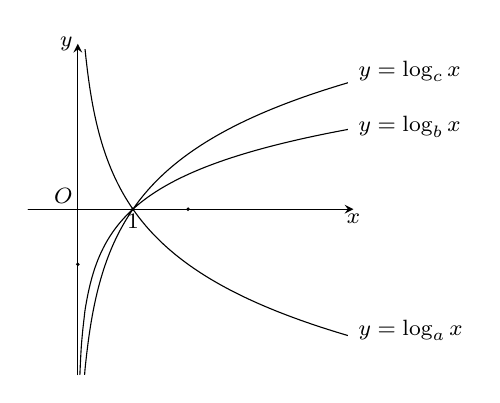
\begin{tikzpicture}[scale=0.7,font=\footnotesize,line join=round,line cap=round,>=stealth]
				\def\xmax{5} \def\ymin{-3} \def\ymax{3} 
				\draw[->] (-0.9,0)--(\xmax,0) node [below]{$x$}; 
				\draw[->] (0,\ymin)--(0,\ymax)  node [left]{$y$};
				\node at (0,0)  [above left]{$O$};
				 \node at (5,-2.2) [right]{$y=\log_ax$};
				 \node at (5,1.5) [right]{$y=\log_bx$};
				\node at  (5,2.5) [right]{$y=\log_cx$};
				\clip (-0.9,\ymin) rectangle  (\xmax-0.1,\ymax-0.1);
				\draw[smooth,samples=300,domain=0.03:\xmax]  plot (\x,{ln(\x)/ln(0.5)})
					plot (\x,{ln(\x)/ln(2)}) plot  (\x,{ln(\x)/ln(3)});
				 \fill (1,0) circle (1.0pt) node[below]{$1$}
					(2,0) circle  (1.0pt)
					(0,-1)  circle (1.0pt);
			\end{tikzpicture}
		} 
	 \loigiai{
		Dựa vào đồ thị ta có hàm số $y=\log_bx$ là một hàm số nghịch biến trên tập xác định của nó nên $0<b<1$; hàm số  $y=\log_ax$; $y=\log_cx$ là các hàm số đồng biến trên tập xác định của nó nên $a>1$ và $c>1$.
		\begin{center}
			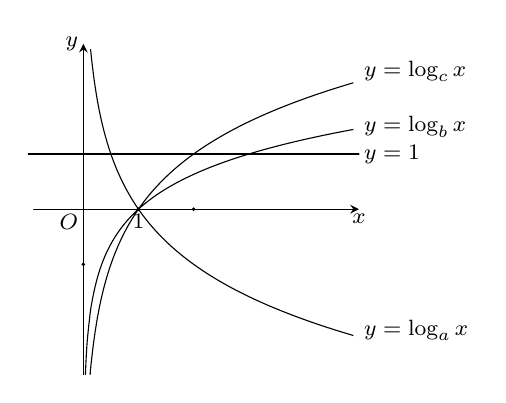
\begin{tikzpicture}[scale=0.7,font=\footnotesize,line join=round,line cap=round,>=stealth]
					 \def\xmax{5} \def\ymin{-3} \def\ymax{3}
					\draw[->]  (-0.9,0)--(\xmax,0) node [below]{$x$};
					\draw[->] (0,\ymin)--(0,\ymax) node  [left]{$y$};
					 \node at (0,0) [below left]{$O$};
					\node  at (5,-2.2) [right]{$y=\log_ax$};
					\node at (5,1.5)  [right]{$y=\log_bx$};
					\node  at (5,2.5) [right]{$y=\log_cx$};
					\draw (-1,1)--(5,1) node[right]{$y=1$}; 
					 \clip (-0.9,\ymin) rectangle (\xmax-0.1,\ymax-0.1);
					\draw[smooth,samples=300,domain=0.03:\xmax]  plot (\x,{ln(\x)/ln(0.5)})
						plot (\x,{ln(\x)/ln(2)}) plot  (\x,{ln(\x)/ln(3)});
					\fill (1,0) circle (1.0pt) node[below]{$1$} 
						 (2,0) circle (1.0pt)
						(0,-1) circle  (1.0pt);
				\end{tikzpicture}
		\end{center}
		Kẻ đường thẳng  $y=1$ cắt đồ thị các hàm số $y=\log_cx$; $y=\log_ax$ lần lượt tại các điểm $A(c; 1)$ và $B(a; 1)$.\\
		Dựa vào đồ thị  ta thấy $x_A<x_B\Leftrightarrow c<a$.\\
	 Vậy $a>c>b$.}
\end{ex}

% từ: cau-hoi/lop11/1D6_Ham_so_mu_va_ham_so_logarit/1D6-3-3_Su_bien_thien_va_do_thi_cua_ham_so_mu_logarit.tex
\begin{ex}%[1D6V3-3]%[ma:c2c25c7d]
	Cho số thực dương $a$ khác $1$. Biết rằng bất kỳ đường thẳng nào vuông góc với trục hoành mà cắt các đồ  thị của hàm số $y=\log _2x$, $y=\log _ax$ và trục hoành lần lượt tại $M$, $N$ và $A$ thì $AM=2AN$ (hình vẽ bên). Tính giá trị của $a$.
	\begin{center}
		\begin{tikzpicture}[>=stealth,line join=round,line cap=round,font=\footnotesize,scale=1]
				\draw  (0,0) node[above left]{$O$};
				 \draw[->] (-1,0)--(5,0) node[right] {$x$};
				\draw[->] (0,-2)--(0,2) node[above] {$y$}; 
				\path (2,0)  coordinate (A)
					(2,1)  coordinate (M)
					(2,-0.5) coordinate (N); 
				\draw [smooth,domain=0.1:5,samples=100]plot (\x,{(ln (\x))/(ln  (0.25))});
				\draw  [smooth,domain=0.3:5,samples=100]plot (\x,{(ln (\x))/(ln (2))});
				\draw (M)--(N); 
				\foreach \d/\g in {A/45,M/150,N/-150} 
				\draw[fill] (\d) circle  (1pt) +(\g:3mm) node{$\d$};
			\end{tikzpicture}
	\end{center}
	\loigiai{ 
		Dựa vào đồ thị  ta thấy $0<a<1$.
		Đường thẳng $x=m$ ($m>0$) cắt đồ thị của hàm số $y=\log_2x$, $y=\log_ax$ và trục hoành lần lượt tại  $M(m;\log_2m)$, $N(m;\log_am)$ và $A(m;0)$.\\
		Theo đề bài  ta có
		\begin{eqnarray*}
			 AM=2AN &\Leftrightarrow &|\log _2m|=2|\log_am|\\
			&\Leftrightarrow &\hoac{&\log_2m=2\log_am\\&\log_2m=-2\log _am}\\  &\Leftrightarrow &\hoac{&a=\sqrt{2}\\&a=\dfrac{1}{4}.}
		\end{eqnarray*}
	Vì  $0<a<1$ nên $a=\dfrac{1}{4}$.}
\end{ex}

% từ: cau-hoi/lop11/1D6_Ham_so_mu_va_ham_so_logarit/1D6-4-2_Phuong_trinh_mu_logarit_co_ban.tex
\begin{ex}%[1D6N4-2]%[ma:5777da2f]
	Phương trình  $2^{x+1}=8$ có nghiệm là
	\choice 
		{$x=0$} 
		{\True  $x=2$}
		 {$x=\dfrac{1}{2}$}
		{$x=1$} 
	\loigiai{ 
		Ta có $2^{x+1}=8 \Leftrightarrow x+1  = 3 \Leftrightarrow x = 2$.
	 }
\end{ex}

% từ: cau-hoi/lop11/1D6_Ham_so_mu_va_ham_so_logarit/1D6-4-2_Phuong_trinh_mu_logarit_co_ban.tex
\begin{bt}%[1D6H4-2]%[ma:85464df2]
	Giải các  phương trình sau
	\begin{multicols}{2}
		\begin{enumerate}
			\item $2^{x+1}=8^{x}$; 
			\item $3^{4^x}=4^{3^x}$; 
			\item  $5^{2x+1}=\left(\dfrac{1}{125}\right)^{x+2}$;
			\item  $2^{x-1}=5^{x^2+2x-3}$;
			\item  $\left(2+\sqrt{3}\right)^{-2x}=\left(2-\sqrt{3}\right)^{x^2}$;
			\item $2^x\cdot  5^x=0{,}2\cdot \left(10^{x-1}\right)^5$.
		\end{enumerate}
	\end{multicols}
	 \loigiai{
		\begin{enumerate}
			\item Ta có $2^{x+1}=8^{x} \Leftrightarrow  x+1=x\log_2 8 \Leftrightarrow x+1=3x \Leftrightarrow x=\dfrac{1}{2}$.\\
			Vậy phương trình  có một nghiệm $x=\dfrac{1}{2}$.
			\item Ta  có
			\begin{eqnarray*}
				&&3^{4^x}=4^{3^x}\\ 
				&\Leftrightarrow& 4^x=3^x\cdot \log_3 4 \\ 
				&\Leftrightarrow& x=\log_4  \left(3^x\cdot \log_3 4\right) \\
				&\Leftrightarrow& x=x\cdot \log_4 3+\log_4\left(\log_3  4\right)\\
				&\Leftrightarrow& x=\dfrac{\log_4\left(\log_3  4\right)}{1-\log_4 3}.
			\end{eqnarray*}
			Vậy phương trình  có một nghiệm $x=\dfrac{\log_4\left(\log_3 4\right)}{1-\log_4 3}$.
			\item Ta có $5^{2x+1}=\left(\dfrac{1}{125}\right)^{x+2} \Leftrightarrow 2x+1=(x+2)\log_5 \dfrac{1}{125}\Leftrightarrow  2x+1=-3x-6\Leftrightarrow x=-\dfrac{7}{5}$.\\
			Vậy phương trình  có một nghiệm $x=-\dfrac{7}{5}$.
			 \item Ta có
			\begin{eqnarray*}
				&&2^{x-1}=5^{x^2+2x-3}\\ 
				&\Leftrightarrow& \log_5 2^{x-1}=\log_5  5^{x^2+2x-3} \\
				 &\Leftrightarrow& (x-1)\log_5 2=x^2+2x-3 \\
				 &\Leftrightarrow& x^2+(2-\log_5 2)x+(\log_5 2 -3)=0 \\
				 &\Leftrightarrow& \hoac{&x=1\\&x=-3+\log_5 2.}
			\end{eqnarray*}
			Vậy  phương trình có hai nghiệm $x=1$, $x=-3+\log_5 2$.
			 \item
			Ta có $(2+\sqrt{3})(2-\sqrt{3})=1  \Rightarrow 2-\sqrt{3}=\dfrac{1}{2+\sqrt{3}}=(2+\sqrt{3})^{-1}$.\\
			 Do đó
			\begin{eqnarray*}
				&&\left(2+\sqrt{3}\right)^{-2x}=\left(2-\sqrt{3}\right)^{x^2} \\ &\Leftrightarrow& -2x=x^2\log_{2+\sqrt{3}} (2-\sqrt{3})  \\
				&\Leftrightarrow& 2x=x^2  \\
				 &\Leftrightarrow& \hoac{&x=0\\&x=2.}\\
			\end{eqnarray*}
			Vậy phương trình có hai  nghiệm $x=0$, $x=2$.
			\item Ta  có
			\begin{eqnarray*}
				&&2^x\cdot 5^x=0{,}2\cdot \left(10^{x-1}\right)^5  \\
				 &\Leftrightarrow& 10^x=0{,}2\cdot 10^{5x-5}\\
				 &\Leftrightarrow& x=\log 0{,}2 +5x-5\\
				&\Leftrightarrow& 4x=6-\log  2\\
				&\Leftrightarrow& x=\dfrac{3}{2}-\dfrac{1}{4}\log 2. 
			\end{eqnarray*}
			Vậy phương trình có một nghiệm $x=\dfrac{3}{2}-\dfrac{1}{4}\log 2$. 
		\end{enumerate}
	 }
\end{bt}

% từ: cau-hoi/lop11/1D6_Ham_so_mu_va_ham_so_logarit/1D6-4-3_Bat_phuong_trinh_mu_logarit_co_ban.tex
\begin{bt}%[1D6N4-3]%[ma:05d54616]
% nguon: Archive/SP-4Phan-Dot3/Data/CTST_1-OTHK2_De05.tex #4198

	Giải bất phương trình $\left(\dfrac{1}{2}\right)^x>32$.
	\loigiai{
		Ta có $\left(\dfrac{1}{2}\right)^x>32\Leftrightarrow \left(\dfrac{1}{2}\right)^x>\left(\dfrac{1}{2}\right)^{-5}\Leftrightarrow x<-5$.\\
		Vậy tập nghiệm của bất phương trình là $S=(-\infty;-5)$.
	}
\end{bt}

% từ: cau-hoi/lop11/1D6_Ham_so_mu_va_ham_so_logarit/1D6-4-5_Bat_phuong_trinh_mu_logarit_dua_ve_cung_co_so.tex
\begin{ex}%[1D6H4-5]%[ma:c215c15d]
	Giải các bất phương trình  sau
	\begin{listEX}[3]
		\item  $3^x\ge 9$;
		 \item $\left(\dfrac{1}{2}\right)^x\le 4$;
		\item  ${2^{x+2}}<\sqrt{2^3}$;
		\item  $2^x>{3^{x+1}}$;
		 \item $\left(\dfrac{1}{2}\right)^x>32$;
		\item  ${3^{x^2-2x}}<27$.
	\end{listEX}
	\loigiai{ 
	\begin{listEX}
		\item Ta có $3^x\ge 9\Leftrightarrow x\ge \log  _39\Leftrightarrow x\ge 2$. Vậy tập nghiệm là $S=\left[2;+\infty\right) $.
		\item Ta có $\left(\dfrac{1}{2}\right)^x\le 4\Leftrightarrow x\ge \log _{\tfrac{1}{2}}4 \Leftrightarrow x\geq -2$. Vậy  tập nghiệm là $S=\left[-2;+\infty\right) $.
		\item Ta  có $2^{x+2}<\sqrt{2^3}\Leftrightarrow 2^{x+2}<2^{\tfrac{3}{2}}\Leftrightarrow x+2<\dfrac{3}{2}\Leftrightarrow x<-\dfrac{1}{2}$.\\
		Vậy tập nghiệm  là $S=\left(-\infty;\dfrac{-1}{2}\right) $.
		\item Ta có $2^x>3^{x+1}\Leftrightarrow 2^x>3\cdot 3^x\Leftrightarrow  \left(\dfrac{2}{3}\right)^x>3\Leftrightarrow x<\log _{\tfrac{2}{3}}3$.\\
		Vậy tập nghiệm là $S=\left(-\infty;\log _{\tfrac{2}{3}}3\right) $. 
		\item Ta có $\left(\dfrac{1}{2}\right)^x>32\Leftrightarrow \left(\dfrac{1}{2}\right)^x>\left(\dfrac{1}{2}\right)^{-5}\Leftrightarrow x<-5$.  Vậy tập nghiệm là $S=\left(-\infty;-5\right) $.
		 \item Ta có $3^{x^2-2x}<27\Leftrightarrow 3^{x^2-2x}<3^3\Leftrightarrow x^2-2x<3\Leftrightarrow x^2-2x-3<0\Leftrightarrow -1<x<3$.\\
		Vậy  tập nghiệm là $S=\left(-1;3\right) $.
	\end{listEX}
	} 
\end{ex}

% từ: cau-hoi/lop11/1D6_Ham_so_mu_va_ham_so_logarit/1D6-4-5_Bat_phuong_trinh_mu_logarit_dua_ve_cung_co_so.tex
\begin{ex}%[1D6V4-5]%[ma:3127377f]
	 Giải các bất phương trình sau
	\begin{listEX}[2]
		\item $3^{2x+1}  -4\cdot 3^x+1>0$;
		\item $9^x - 5 \cdot  3^x +6 <0$.
	\end{listEX}
	 \loigiai{
		\begin{listEX}
			 \item Ta có $3^{2x+1}-4\cdot 3^x+1>0 \Leftrightarrow 3\cdot 3^{2x}-4\cdot 3^x+1>0$.\\
			Đặt $t=3^x$, $t>0$, bất phương trình trên  trở thành $$3t^2-4t+1>0 \Leftrightarrow \hoac{&t>1\\&t<\dfrac{1}{3}.}$$
			 Với $t>1$, ta có $3^x>1 \Leftrightarrow x >0$.\\
			Với $t<-1$, ta có $3^x<\dfrac{1}{3} \Leftrightarrow x<-1$.\\ 
			Vậy tập nghiệm của bất  phương trình là $S=(-\infty;-1)\cup (1;+\infty)$.
			\item Ta có $9^x-5  \cdot 3^x+6<0 \Leftrightarrow \left(3^2\right)^x-5\cdot 3^x+6<0 \Leftrightarrow \left(3^x\right)^2 -5 \cdot 3^x+6<0. \quad (*)$\\
			Đặt $t=3^x$, $t>0$, bất phương trình $(*)$ trở thành $$t^2-5t+6<0 \Leftrightarrow 2<t<3.$$ 
			Với  $2<t<3$ ta có $2<3^x<3 \Leftrightarrow \log_3 2 <x<1$.\\
			Vậy tập nghiệm  của bất phương trình là $S=\left(\log_3 2;1\right)$.
		\end{listEX}
	} 
\end{ex}

% từ: cau-hoi/lop11/1D7_Dao_ham/1D7-1-1_Tinh_dao_ham_bang_dinh_nghia.tex
\begin{ex}%[1D7V1-1]%[ma:a8bdeab2]
	Cho hàm số $f(x)=\heva{&\dfrac{3-\sqrt{4-x}}{4}&\text{  khi }x\ne 0 \\
	&{\dfrac{1}{4}}&\text{ khi }x=0}$. Tính $f'(0)$ (kết quả làm tròn đến hàng phần trăm). 
	 \shortans{0,06}
	 \loigiai{
		Với $x\ne 0$ xét 
		\begin{eqnarray*}
			\lim\limits_{x\to 0}\dfrac{f(x)-f(0)}{x-0}&=&\lim\limits_{x\to 0}\dfrac{\tfrac{3-\sqrt{4-x}}{4}-\tfrac{1}{4}}{x}\\ 
			&=&\lim\limits_{x\to 0}\dfrac{2-\sqrt{4-x}}{4x}\\ 
			 &=&\lim\limits_{x\to 0}\dfrac{1}{4\left(2+\sqrt{4-x}\right)}\\
			 &=&\dfrac{1}{16}.
		\end{eqnarray*}
		Vậy $f'(0)\approx  0{,}06$.
	} 
\end{ex}

% từ: cau-hoi/lop11/1D7_Dao_ham/1D7-1-4_Y_nghia_Vat_ly_cua_dao_ham.tex
\begin{ex}%[1D7V1-4]%[ma:36054570]
	Một chất điểm chuyển động có quãng đường được cho bởi phương trình $s(t)=t^{3}-3t^{2}+5t+10$, trong đó $t>0$ với $t$ tính bằng giây và $s$ tính bằng mét.  Hỏi tại thời điểm vận tốc của vật đạt giá trị nhỏ nhất thì quãng đường vật đi được bằng bao nhiêu?
	 \choice
		{\True $13$ m} 
		{$3$  m}
		{$16$ m} 
		 {$10$ m}
	 \loigiai{
		\begin{itemize}
			\item Vận tốc  của chuyển động là $v(t)=s'(t)=3t^{2}-6t+5$.
			\item Ta có  $v(t)=3(t-1)^{2}+2 \ge 2$. Dấu \lq\lq$=$\rq\rq\, xảy ra khi $t=1$.
			\item Vận tốc  đạt giá trị nhỏ nhất tại $t=1$ s.
			\item Khi đó, quãng đường vật đi được là  $s(1)=1^3-3(1)^2+5(1)+10 = 13$ (m).
		\end{itemize}
	 }
\end{ex}

% từ: cau-hoi/lop11/1D7_Dao_ham/1D7-1-4_Y_nghia_Vat_ly_cua_dao_ham.tex
\begin{ex}%[1D7V1-4]%[ma:e18ca3b1]
	Một chất điểm chuyển động có phương trình chuyển động là $s(t)=t^2+4t+6$ ($t$ được tính bằng giây, $s$ được tính bằng mét). Tính vận tốc tức thời của chuyển  động tại thời điểm $t=5$\,s.
	 \shortans{14}
	 \loigiai{
		Vận tốc tức thời của chuyển động tại thời điểm $t=5$ là 
		\begin{eqnarray*}
			v(5)=s'(5)&=&\lim\limits_{t\to 5} \dfrac{s(t)-s(5)}{t-5}\\ 
			 &=&\lim\limits_{t\to 5}\dfrac{t^2+4t+6-51}{t-5}\\
			&=&\lim\limits_{t\to  5} \dfrac{t^2+4t-45}{t-5}\\
			 &=&\lim\limits_{t\to 5}\left(t+9\right)\\
			&=&14\text{  (m/s)}.
		\end{eqnarray*}
	} 
\end{ex}

% từ: cau-hoi/lop11/1D7_Dao_ham/1D7-2-1_Tinh_dao_ham.tex
\begin{ex}%[1D7V2-1]%[ma:e36ae0b1]
 Cho hàm số $ y=5\cot x-3 $. 
 \choiceTF 
  {\True $  y'=-5(\cot^2 x+1) $}
  {\True $  y'=\dfrac{-5}{\sin^2{x}}$}
  {$ y'\left(\dfrac{\pi}{2}\right)=5$} 
  {\True $ y\left(\dfrac{\pi}{3}\right)=-\dfrac{9+5\sqrt{3}}{3}$} 
 \loigiai{ 
  \begin{itemchoice}
    \itemch Đúng\\
   Ta có $ y'=\dfrac{-5}{\sin^2{x}}=-5(\cot^2  x+1)$.
   \itemch Đúng\\ 
   Vì  $ y'=\dfrac{-5}{\sin^2{x}}$.
    \itemch Sai\\
    Ta có $ y'=\dfrac{-5}{\sin^2{x}}$.\\
   Suy ra $y'\left(\dfrac{\pi}{2}\right)=-5 $. 
   \itemch  Đúng\\
   Vì  $ y\left(\dfrac{\pi}{3}\right)=5\cot\left(\dfrac{\pi}{3}\right)-3=-\dfrac{9+5\sqrt{3}}{3}$.
  \end{itemchoice}
 } 
\end{ex}

% từ: cau-hoi/lop11/1D7_Dao_ham/1D7-2-1_Tinh_dao_ham.tex
\begin{bt}%[1D7H2-1]%[ma:34e60620]
% nguon: Archive/2024/TOAN_11_XE/TOAN_11_XE/data4/11C9/KNTT-9.2.tex #1305

	Tính đạo hàm của các hàm số sau:
	\begin{listEX}[3]
		\item $y=3x^2-4x+2$;
		\item $y=x\sin x$;
		\item $y=\dfrac{3x+2}{2x-1}$.
	\end{listEX}
	\loigiai{
		\begin{listEX}
			\item $y=3x^2-4x+2$.\\
			$y'=\left(3x^2-4x+2\right)^\prime=\left(3x^2\right)^\prime-\left(4x\right)^\prime+(2)^\prime=3\left(x^2\right)^\prime-4\left(x\right)^\prime+0=3\cdot2x-4\cdot 1=6x-4$.
			\item $y=x\sin x$.\\
			$y'=\left(x\sin x\right)^\prime=\left(x\right)'\sin x+x \left(\sin x\right)'=1\cdot \sin x+x \cdot \cos x=\sin x+x\cos x$.
			\item $y=\dfrac{3x+2}{2x-1}$.
			\begin{eqnarray*}
				y'&=&\left(\dfrac{3x+2}{2x-1}\right)^\prime=\dfrac{\left(3x+2\right)'\left(2x-1\right)-\left(3x+2\right)\left(2x-1\right)'}{\left(2x-1\right)^2}\\
				&=&\dfrac{3\cdot \left(2x-1\right)-(3x+2)\cdot 2}{\left(2x-1\right)^2}
				=\dfrac{6x-3-6x-4}{\left(2x-1\right)^2}=\dfrac{-7}{\left(2x-1\right)^2}.
			\end{eqnarray*}
	\end{listEX}}
\end{bt}

% từ: cau-hoi/lop11/1D7_Dao_ham/1D7-2-1_Tinh_dao_ham.tex
\begin{bt}%[1D7H2-1]%[ma:c09ce59d]
% nguon: Archive/2024/TOAN_11_XE/TOAN_11_XE/data4/11C9/KNTT-9.2.tex #1309

	Tính đạo hàm của các hàm số sau:
	\begin{listEX}[3]
		\item $y=\left(2x^3+3\right)^2$;
		\item $y=\cos 3x$;
		\item $y=\log_2\left(x^2+2\right)$.
	\end{listEX}
	\loigiai{
		\begin{enumerate}
			\item $y=\left(2x^3+3\right)^2$.\\
			Đặt $u=2x^3+3$ thì $y=u^2$. Ta có $u'_x=6x$ và $y'_u
			=2u$.\\
			Suy ra $y'_x=y'_u\cdot u'_x=2u\cdot 6x=2\left(2x^3+3\right)\cdot 6x =12x\left(2x^3+3\right)$.\\
			Vậy $y'=12x\left(2x^3+3\right)$.
			\item $y=\cos 3x$.\\
			Đặt $u=3x$ thì $y=\cos u$. Ta có $u'_x=3$ và $y'_u
			=-\sin u$.\\
			Suy ra $y'_x=y'_u\cdot u'_x=\left(-\sin u\right)\cdot 6=\left(-\sin 3x\right)\cdot 3 =-3\sin 3x$.\\
			Vậy $y'=-3\sin 3x$.
			\item $y=\log_2\left(x^2+2\right)$.\\
			Đặt $u=x^2+2$ thì $y=\log_2 u$. Ta có $u'_x=2x$ và $y'_u
			=\dfrac{1}{u\ln 2}$.\\
			Suy ra $y'_x=y'_u\cdot u'_x=\dfrac{1}{u\ln 2} \cdot 2x=\dfrac{1}{\left(x^2+2\right)\ln2}\cdot 2x=\dfrac{2x}{\left(x^2+2\right)\ln 2}$.\\
			Vậy $y'=\dfrac{2x}{\left(x^2+2\right)\ln 2}$.
	\end{enumerate}}
\end{bt}

% từ: cau-hoi/lop11/1D7_Dao_ham/1D7-2-1_Tinh_dao_ham.tex
\begin{bt}%[1D7H2-1]%[ma:9fc5bc59]
% nguon: Archive/2024/TOAN_11_XE/TOAN_11_XE/data4/11C9/KNTT-9.OTC.tex #1336
%[Tăng Xuân Phú]
	Tính đạo hàm của các hàm số sau
	\begin{multicols}{3}
	\begin{enumerate}
		\item $y=3 x^4-7 x^3+3 x^2+1$
		\item $y=\left(x^2-x\right)^3$
		\item $y=\dfrac{4 x-1}{2 x+1}$.
	\end{enumerate}
	\end{multicols}	
	\loigiai{Đạo hàm của các hàm số sau là
		\begin{enumerate}
			\item $y^\prime=12x^3-21x^2+6x$.
			\item $y^\prime=3(x^2-x)^2(x^2-x)^\prime=3(x^2-x)^2(2x-1)$.
			\item $y^\prime=\dfrac{(4x-1)^\prime\cdot(2x+1)-(2x+1)^\prime\cdot(4x-1)}{(2x+1)^2}=\dfrac{6}{(2x+1)^2}$.
	\end{enumerate}}
\end{bt}

% từ: cau-hoi/lop11/1D7_Dao_ham/1D7-3-2_Dang_thuc_co_va.tex
\begin{ex}%[1D7V3-2]%[ma:8d1c9ecb]
	Cho $y=\sqrt{2x-x^2}$, tính giá  trị biểu thức $A=y^3\cdot y''$.
	\choice 
		 {$1$}
		{$0$} 
		 {\True $-1$}
		 {$2$}
	 \loigiai{
		Ta có $y'=\dfrac{1-x}{\sqrt{2x-x^2}}$  và $y''=\dfrac{-1}{\left(\sqrt{2x-x^2}\right)^3}$.\\
		 Vậy $A=y^3\cdot y''=\left(\sqrt{2x-x^2}\right)^3\cdot\dfrac{-1}{\left(\sqrt{2x-x^2}\right)^3}=-1$.
	} 
\end{ex}

% từ: cau-hoi/lop11/1D9_Xac_suat/1D9-2-3_Quy_tac_cong_cho_hai_bien_co_xung_khac.tex
\begin{bt}%[1D9V2-3]%[ma:7132dd73]
% nguon: Archive/SP-4Phan-Dot3/Data/CTST_1-OTHK2_De01.tex #4229
%[Câu 4]
	Một xạ thủ bắn vào một tấm bia biết xác suất bắn trúng vòng tròn $10$ là $0{,}2$; vòng $9$ là $0{,}25$ và vòng $8$ là $0{,}15$. Nếu trúng vòng $k$ thì được $k$ diểm. Giả sử xạ thủ đó bắn ba phát súng một cách độc lập. Xạ thủ đạt loại Giỏi nếu anh ta đạt ít nhất $28$ điểm. Tính xác suất để xạ thủ này đạt loại Giỏi.
	\loigiai{
		Gọi $H$ là biến cố \lq\lq Xạ thủ bắn đạt loại Giỏi\rq\rq\, và $A$, $B$, $C$, $D$ là các biến cố sau: 
		\begin{itemize}
			\item $A$ là biến cố \lq\lq Ba viên trúng vòng $10$\rq\rq.
			\item $B$ là biến cố \lq\lq Hai viên trúng vòng $10$ và một viên trúng vòng $9$\rq\rq.
			\item $C$ là biến cố \lq\lq Một viên trúng vòng $10$ và hai viên trúng vòng $9$\rq\rq.
			\item $D$ là biến cố \lq\lq Hai viên trúng vòng $10$ và một viên trúng vòng $8$\rq\rq.
		\end{itemize}
		Khi đó $A$, $B$, $C$, $D$ là các biến cố đôi một xung khắc và $H=A \cup B \cup C \cup D$.\\
		Theo quy tắc cộng xác suất $\mathrm{P}(H)=\mathrm{P}(A)+\mathrm{P}(B)+\mathrm{P}(C)+\mathrm{P}(D)$.\\ 
		Mặt khác		
		\begin{eqnarray*}
			\mathrm{P}(A)&=&0{,}2 \cdot 0{,}2 \cdot 0{,}2=0{,}008. \\
			\mathrm{P}(B)&=&0{,}2 \cdot 0{,}2 \cdot 0{,}25+0{,}2 \cdot 0{,}25 \cdot 0{,}2+0{,}2 \cdot 0{,}25 \cdot 0{,}2=0{,}03. \\
			\mathrm{P}(C)&=&0{,}2 \cdot 0{,}25 \cdot 0{,}25+0{,}25 \cdot 0{,}2 \cdot 0{,}25+0{,}25 \cdot 0{,}25 \cdot 0{,}2=0{,}0375. \\
			\mathrm{P}(D)&=&0{,}2 \cdot 0{,}2 \cdot 0{,}15+0{,}2 \cdot 0{,}15 \cdot 0{,}2+0{,}15 \cdot 0{,}2 \cdot 0{,}2=0{,}018.
		\end{eqnarray*}		
		Vậy xác suất để xạ thủ này đạt loại Giỏi là 
		$$\mathrm{P}(H)=0{,}008+0{,}03+0{,}0375+0{,}018=0{,}0935.$$
	}
\end{bt}

% từ: cau-hoi/lop11/1H4_Duong_thang_mat_phang_Quan_he_song_song/1H4-1-1_Cau_hoi_ly_thuyet.tex
\begin{ex}%[1H4N1-1]%[ma:07895e01]
	\immini{ 
	Cho hình chóp $S.ABCDE$, số mặt của hình chóp  đó là bao nhiêu?
	\choice 
		{$4$} 
		{$7$} 
		{$5$} 
		{\True  $6$}
		} 
		{\begin{tikzpicture}[line join=round,line cap=round]
		\coordinate (S) at (1,4); 
		\coordinate (A) at  (0,0);
		\coordinate (B) at  (1,-2);
		\coordinate  (C) at (3,-3);
		 \coordinate (E) at (5,0);
		\coordinate (D) at  (4,-2);
		\draw  (S)--(A)
			(S)--(B) 
			 (S)--(C)
			 (S)--(D)
			 (S)--(E)
			 (A)--(B)--(C)--(D)--(E);
		 \draw[dashed,thin](A)--(E);
		\foreach \i/\g in {S/90,A/180,B/-90,C/-90,D/-30,E/0}{\draw[fill=black](\i) circle  (1pt)
			($(\i)+(\g:3mm)$) node[scale=1]{$\i$};} 
	\end{tikzpicture}
		} 
	 \loigiai{
	 Hình chóp $S.ABCDE$ có 6 mặt.}
\end{ex}

% từ: cau-hoi/lop11/1H4_Duong_thang_mat_phang_Quan_he_song_song/1H4-1-2_Hinh_bieu_dien_cua_mot_hinh_khong_gian.tex
\begin{ex}%[1H4N1-2]%[ma:b4dde02a]
	Trong các hình vẽ sau hình nào có thể là hình biểu diễn  của một hình tứ diện?
	\begin{center}
		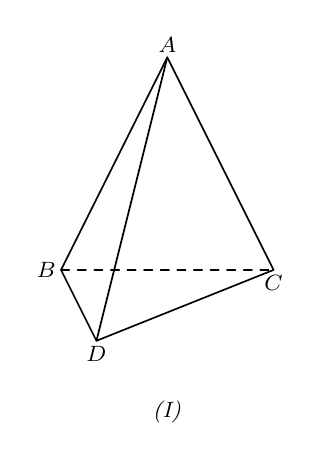
\begin{tikzpicture}[line join=round,line cap=round,line width=.6pt,font=\footnotesize,scale=0.9]
				\coordinate[label=left:$B$] (B) at (0,0); 
				\coordinate[label=below:$C$] (C) at  (3,0);
				\coordinate[label=below:$D$] (D)  at (0.5,-1);
				\coordinate[label=above:$A$] (A) at (1.5,3); 
				 \draw (A)--(B)--(D)--(C)--cycle;
				\draw  (A)--(D);
				 \draw[dashed] (B)--(C);
				\node at (1.5,-2)  {\textit{(I)}};
			\end{tikzpicture}
		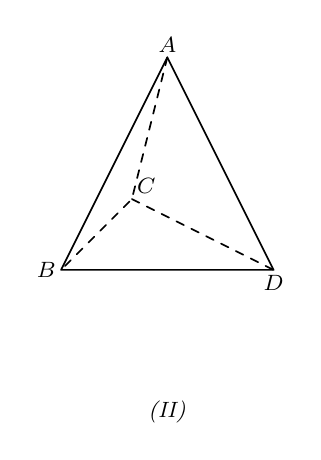
\begin{tikzpicture}[line join=round,line cap=round,line width=.6pt,font=\footnotesize,scale=0.9]
				\coordinate[label=left:$B$]  (B) at (0,0);
				\coordinate[label=below:$D$] (D)  at (3,0);
				\coordinate[label=above right:$C$] (C) at (1,1); 
				\coordinate[label=above:$A$]  (A) at (1.5,3);
				\draw  (A)--(B)--(D)--cycle;
				\draw[dashed]  (C)--(D)
					 (A)--(C)--(B);
				 \node at (1.5,-2) {\textit{(II)}};
			\end{tikzpicture}
		\begin{tikzpicture}[line join=round,line cap=round,line width=.6pt,font=\footnotesize,scale=0.9]
				\coordinate[label=left:$B$] (B) at (0,0); 
				\coordinate[label=below:$C$] (C) at  (3,0);
				\coordinate[label=below right:$D$]  (D) at (4,0);
				\coordinate[label=above:$A$] (A) at (1,3); 
				\draw (A)--(B)--(D)--cycle; 
				 \draw (A)--(C);
				\node at  (1.5,-2) {\textit{(III)}};
			\end{tikzpicture}
		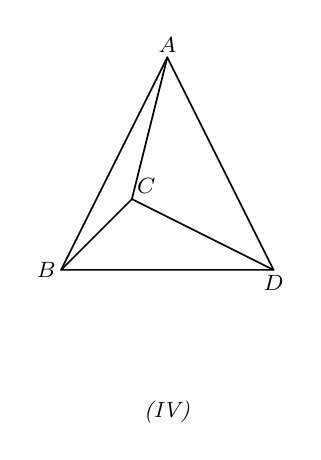
\begin{tikzpicture}[line join=round,line cap=round,line width=.6pt,font=\footnotesize,scale=0.9]
				\coordinate[label=left:$B$] (B)  at (0,0);
				\coordinate[label=below:$D$] (D) at  (3,0);
				\coordinate[label=above right:$C$]  (C) at (1,1);
				\coordinate[label=above:$A$] (A)  at (1.5,3);
				\draw  (A)--(B)--(D)--cycle;
				 \draw (A)--(C)--(D)
					(B)--(C); 
				 \node at (1.5,-2) {\textit{(IV)}};
			\end{tikzpicture}
	\end{center}
	 \choice
		{\True $(I),\,(II),\,(IV)$} 
		 {$(I),\,(II),\,(III),\,(IV)$}
		{$  (I)$}
		{$  (I),\,(II),\,(III)$}
	\loigiai{ 
	Hình $ (III)$ không phải là hình biểu  diễn của một hình tứ diện.}
\end{ex}

% từ: cau-hoi/lop11/1H4_Duong_thang_mat_phang_Quan_he_song_song/1H4-6-5_Tinh_ti_so_doan_thang_dien_tich_qua_phep_chie.tex
\begin{ex}%[1H4V6-5]%[ma:b88c6ba1]
	Cho hình chóp $S. ABCD$ có đáy $ABCD$ là hình bình hành. Gọi $M$, $P$ lần lượt là trung điểm của các cạnh $SA$ và $SC$. Điểm $N$ thuộc cạnh $SB$ sao cho $\dfrac{SN}{SB}=\dfrac{2}{3}$. Gọi $Q$ là giao điểm của cạnh $SD$ và mặt phẳng $(MNP)$. Tính tỉ số $\dfrac{SQ}{SD}$ (kết quả làm tròn tới  hàng phần chục)
	 \shortans{0,4}
	 \loigiai{
		\begin{center}
			\begin{tikzpicture}[scale=2.1,font=\footnotesize,line join=round,line cap=round,>=stealth]
					\coordinate (A) at  (0,0);
					\coordinate  (B) at (1.7,-0.3);
					\coordinate  (D) at (1,1.2);
					 \coordinate (C) at ($(B)+(D)-(A)$);
					\coordinate (S)  at (1.2,2.8);
					\coordinate  (M) at ($(S)!0.5!(A)$);
					\coordinate (P)  at ($(S)!0.5!(C)$);
					\coordinate (N)  at ($(S)!2/3!(B)$);
					 \coordinate (Q) at ($(S)!0.4!(D)$);
					\coordinate (O) at (intersection  cs: first line={(A)--(C)},second line={(B)--(D)});
					\coordinate (I) at (intersection cs:  first line={(M)--(P)},second line={(N)--(Q)});
					 \draw (S)--(B)
						 (S)--(C)
						(B)--(C) 
						(A)--(B) 
						(S)--(A); 
					\draw[dashed] (S)--(D) 
						 (C)--(D)
						 (D)--(A)
						(M)--(N) 
						 (N)--(P)
						 (P)--(M)
						 (M)--(Q)
						 (N)--(Q)
						(P)--(Q) 
						(A)--(C) 
						(B)--(D) 
						 (N)--(Q);
					\foreach  \pt in {A,B,C,D,S,M,N,P,Q,O,I}
					\filldraw (\pt) circle  (0.5pt);
					\node[below left] at (A)  {A};
					\node[below right] at (B)  {B};
					\node[below right]  at (C) {C};
					 \node[above right] at (D) {D};
					 \node[above] at (S) {S};
					\node[left] at (M)  {M};
					\node[above  right] at (N) {N};
					 \node[right] at (P) {P};
					\node[left] at  (Q) {Q};
					\node[below] at (O) {O}; 
					 \node[above left] at (I) {I};
				\end{tikzpicture}
		\end{center}
		Trong $(ABCD)$, gọi $O$ là giao điểm của $AC$ và $BD$, $I$ là giao điểm của $MP$ và $SO$.\\ 
		Trong $(SBD)$ gọi $Q$ là giao điểm của $NI$ với $SD$.\\  Khi đó $\heva{&Q\in SD\\
		&Q\in NI\subset (MNPQ)} \Rightarrow  Q=SD\cap (MNP)$.\\
		 Vì $M$ và $P$ lần lượt là trung điểm $SA$, $SC$ nên $MP$ cũng đi qua trung điểm của $SO$, do đó $I$ là trung điểm của $SO$.\\
		Đặt $\dfrac{SQ}{SD}=k$, khi đó $\overrightarrow{SQ}=k \overrightarrow{SD}$. Ta có 
		 \[\overrightarrow{SO}=\dfrac{1}{2}\left(\overrightarrow{SB}+\overrightarrow{SD}\right).\]
		$I$ là trung điểm $SO$  nên
		\[\overrightarrow{SI}=\dfrac{1}{2}\overrightarrow{SO}=\dfrac{1}{4}\left(\overrightarrow{SB}+\overrightarrow{SD}\right).\] 
		$N$ chia $SB$ theo $\dfrac{SN}{SB}=\dfrac{2}{3}$ nên 
		 \[\overrightarrow{SN}=\dfrac{2}{3}\overrightarrow{SB}.\]
		Vì $Q$ là giao điểm của $SD$ với  $NI$, nên tồn tại $t\in\mathbb{R}$ sao cho
		 \[\overrightarrow{SQ}=(1-t)\overrightarrow{SN}+t\overrightarrow{SI}.\]
		Thay các biểu thức trên  vào, ta được
		 \[k\overrightarrow{SD}=(1-t)\cdot\dfrac{2}{3}\overrightarrow{SB}+t\cdot\dfrac{1}{4}\left(\overrightarrow{SB}+\overrightarrow{SD}\right).\]
		\[k\overrightarrow{SD}=\left[\dfrac{2(1-t)}{3}+\dfrac{t}{4}\right]\overrightarrow{SB}+\dfrac{t}{4}\overrightarrow{SD}.\] 
		 So sánh hệ số hai vế, ta có
		\[k=\dfrac{t}{4},  \qquad \dfrac{2(1-t)}{3}+\dfrac{t}{4}=0.\]
		 Giải phương trình:
		 \[\dfrac{2(1-t)}{3}+\frac{t}{4}=0
		 \Leftrightarrow \dfrac{8(1-t)}{12}+\frac{3t}{12}=0
		\Leftrightarrow  8(1-t)+3t=0
		 \Leftrightarrow t=\dfrac{8}{5}.\]
		 Suy ra
		\[k=\frac{t}{4}=\dfrac{8}{5  \cdot 4}=\dfrac{2}{5}.\]
		Vậy  $\dfrac{SQ}{SD}=\dfrac{2}{5}$.
	} 
\end{ex}

% từ: cau-hoi/lop11/1H8_Quan_he_vuong_goc_trong_khong_gian/1H8-1-3_Tim_goc_giua_hai_duong_thang.tex
\begin{ex}%[1H8H1-3]%[ma:57ed7e15]
	Cho hình lập phương $ABCD.A'B'C'D'$ cạnh $a$, $M$ là trung điểm $CD$.  Gọi $\alpha$ là góc tạo bởi $A'B$ và $D'M$. Tính $\cos \alpha$.
	\choice 
		{$\cos  \alpha=\dfrac{1}{2}$}
		 {\True $\cos \alpha=\dfrac{3\sqrt{5}}{5}$}
		{$\cos  \alpha=\dfrac{\sqrt{2}}{2}$}
		{$\cos  \alpha=\dfrac{\sqrt{10}}{10}$}
	 \loigiai{
	 \immini{
		Ta có $D'C\parallel A'B$ nên $(A'B,D'M)=(D'C,D'M)=\alpha$. \\ 
		Có $D'M=\dfrac{a\sqrt{5}}{2}$, $D'C=a\sqrt{2}$,  $CM=\dfrac{a}{2}$. \\
		Tam giác  $D'MC$ có $$\cos \alpha=\dfrac{D'M^2+D'C^2-CM^2}{2D'M.D'C}=\dfrac{3\sqrt{5}}{5}.$$
		}{ 
		\begin{tikzpicture}[scale=0.6,font=\footnotesize,line join=round,line cap=round,>=stealth]
				\coordinate (a) at (2,2); 
				\coordinate (b) at  (0,0);
				\coordinate (c) at (5,0); 
				\coordinate (d) at  (7,2);
				\coordinate  (a1) at ($(a)+(0,5)$);
				 \coordinate (b1) at ($(b)+(0,5)$);
				\coordinate  (c1) at ($(c)+(0,5)$);
				\coordinate (d1)  at ($(d)+(0,5)$);
				\coordinate  (m) at ($(c)!0.5!(d)$);
				\draw[dashed] (b) -- (a) -- (d) 
					(a)  -- (a1);
				\draw (b) -- (c) -- (d) -- (d1) -- (c1) -- (b1)  -- (a1) -- (d1)
					(b) --  (b1)
					(c)  -- (c1);
				\draw (a) node[below]{$A$}; 
				\draw  (b) node[below]{$B$};
				\draw (c)  node[below]{$C$};
				\draw (d)  node[right]{$D$};
				\draw (a1) node[above]{$A'$}; 
				\draw  (b1) node[below left]{$B'$};
				\draw (c1) node[below right]{$C'$}; 
				\draw  (d1) node[right]{$D'$};
				\draw (m)  node[right]{$M$};
				 \draw[dashed] (a1)-- (b);
				\draw (m) -- (d1) -- (c); 
			\end{tikzpicture}
		 }
	 }
\end{ex}

% từ: cau-hoi/lop11/1H8_Quan_he_vuong_goc_trong_khong_gian/1H8-1-3_Tim_goc_giua_hai_duong_thang.tex
\begin{bt}%[1H8H1-3]%[ma:a93bc5d7]
% nguon: Archive/SP_SauLuoi_2024-2025/Sp_GHKII/data/GHKII/1-TN-DS-TLN-TL-THPT-ThiXaQuangTri-QuangTri-GHKII-NH24-25.tex #147
 %[Dự án đề GHKII THPT Thị Xã Quảng Trị - Quảng Trị - 24-25][Lê Phúc]
\immini{Khung của một mái nhà được ghép các thanh gỗ như hình bên. Cho biết tam giác $ABC$ vuông cân tại $A$. Tính góc giữa hai thanh gỗ $a$ và $b$ $(b\equiv BC)$.}
{
\begin{tikzpicture}[scale=0.6, font=\footnotesize, line join=round, line cap=round, >=stealth]
	\coordinate (A1) at (-3,1);
	\coordinate (A2) at (1,-1);
	\coordinate (A3) at (6,1);
	\coordinate (A4) at (2,2);
	\coordinate (A) at (4,5);
	\coordinate (B) at (3,3);
	\coordinate (D) at (6,3.3);
	\coordinate (A7) at (-1,5);
	\coordinate (C) at (intersection of A--A3 and B--D);
	\coordinate (A5) at (3,0.5);
	\coordinate (A6) at (1,-2);
	\coordinate (E) at ($(A7)!0.6!(A)$);
	\coordinate (F) at ($(A1)!0.6!(A2)$);
	\coordinate (G) at ($(A7)!0.3!(A)$);
	\coordinate (H) at ($(A1)!0.3!(A2)$);
	\coordinate (K) at ($(A7)!0.75!(A)$);
	\coordinate (L) at ($(A1)!0.75!(A2)$);
	\coordinate (A9) at ($(A7)!0.15!(A)$);
	\coordinate (A10) at ($(A1)!0.15!(A2)$);
	\coordinate (A11) at ($(A7)!0.45!(A)$);
	\coordinate (A12) at ($(A1)!0.45!(A2)$);
	\coordinate (A13) at ($(A7)!0.85!(A)$);
	\coordinate (A14) at ($(A1)!0.85!(A2)$);
	\coordinate (A15) at ($(A4)!0.15!(A3)$);
	\coordinate (A16) at ($(A4)!0.3!(A3)$);
	\coordinate (A17) at ($(A4)!0.6!(A3)$);
	\coordinate (A18) at ($(A4)!0.75!(A3)$);
	\coordinate (A19) at ($(A4)!0.85!(A3)$);
	\draw[brown,fill=lightgray](A1)--(A2)--(A3)--(A4)--cycle;
	\draw[fill=magenta](0,1)--(-0.5,1)--(-0.5,5.5)--(0,5.5)--cycle;
	\draw[brown](A)--(A7) (A7)--(A1)  (B)--(D) (A4)--(A7) (A)--(A2) (A3)--(A) (G)--(H) (K)--(L) (A9)--(A10) (A11)--(A12) (A13)--(A14) (A17)--(E) (A16)--(G) (A18)--(K) (A15)--(A9) (A19)--(A13);
	\draw[blue,very thick](F)--(E) node [above right]{$a$};
	\draw[blue,very thick](A3)--(A) (A2)--(A);
	\draw[blue,very thick] (B) -- (C) node[midway, above] {$b$};
	\foreach \i/\g in {B/180,C/45,A/90}{\draw[fill=blue](\i) circle (1pt) ($(\i)+(\g:3mm)$) node[scale=1]{$\i$};}
\end{tikzpicture}
}
	\loigiai{
	Do tam giác $ABC$ vuông cân tại $A$ nên $\widehat{ABC}=45^\circ$.\\
	Suy ra $(AB,BC)=45^\circ$.\\
	Do đó $(a,b)=(AB,BC)=45^\circ$.
	}
\end{bt}

% từ: cau-hoi/lop12/2D1_Ung_dung_dao_ham_de_khao_sat_ham_so/2D1-1-1_Xet_tinh_don_dieu_cua_ham_so_cho_boi_cong_thu.tex
\begin{bt}%[2D1H1-1]%[ma:20251975]
% nguon: Archive/2024/0. [LVH] BG - 12 New - 4in1-20240625T224301Z-001/0. [LVH] BG - 12 New - 4in1/2. [LVH] TEX SGK 12 NEW-20240418T074833Z-001/2. [LVH] TEX SGK 12 NEW/[LVH] SGK-12-KNTT/data/C1/12-SGK-KNTT-1-1.tex #1117

	Xét chiều biến thiên của các hàm số sau:
	\begin{multicols}{2}	
		\begin{enumerate}[a)]	
			\item $y=\sqrt{4-x^2}$;
			\item $y=\frac{x}{x^2+1}$.
		\end{enumerate}
	\end{multicols}
	\loigiai{
		\begin{enumerate}[a)]	
			\item $y=\sqrt{4-x^2}$.\\
			Hàm số đã cho có tập xác định là $\left[-2; 2\right]$.\\
			Ta có: $y'=\frac{-x}{\sqrt{4-x^2}}$.\\
			$y'=0\Leftrightarrow x=0$. \\
			Bảng biến thiên của hàm số như sau:
			\begin{center}
				
\begin{tikzpicture}[font=\footnotesize,thick,>=stealth]
					\tikzset{double style/.append style={double distance=1.5pt}}
					\tkzTabInit[nocadre=false,lgt=1.2,espcl=2.5,deltacl=0.6,lw=.75pt,color,colorL=green!50,colorV=green!50]
					{$x$ /0.8,$y'$ /0.6,$y$ /2}
					{$-2$,$0$,$2$}
					\tkzTabLine{ ,+,z,-, }
					\tkzTabVar{-/$0$,+/$2$,-/$0$}
				\end{tikzpicture}
			\end{center}	
			Vậy hàm số đồng biến trên  khoảng $\left(-2;0\right)$ ; nghịch biến trên khoảng  $\left(0;2\right)$.
			\item $y=\frac{x}{x^2+1}$.\\
			Hàm số đã cho có tập xác định là $\mathbb{R}$.\\
			Ta có: $y'=\frac{-x+1}{\left(x^2+1\right)^2}$.\\
			$y'=0\Leftrightarrow x=1$. \\
			Bảng biến thiên của hàm số như sau:
			\begin{center}
				
\begin{tikzpicture}[font=\footnotesize,thick,>=stealth]
					\tikzset{double style/.append style={double distance=1.5pt}}
					\tkzTabInit[nocadre=false,lgt=1.2,espcl=2.5,deltacl=0.6,lw=.75pt,color,colorL=green!50,colorV=green!50]
					{$x$ /0.8,$y'$ /0.6,$y$ /2}
					{$-\infty$,$1$,$+\infty$}
					\tkzTabLine{ ,+,z,-, }
					\tkzTabVar{-/$0$,+/$\frac{1}{2}$,-/$0$}
				\end{tikzpicture}
			\end{center}	
			Vậy hàm số đồng biến trên  khoảng $\left(-\infty;1\right)$ ; nghịch biến trên khoảng  $\left(1;+\infty\right)$.    
		\end{enumerate} 
	}
\end{bt}

% từ: cau-hoi/lop12/2D1_Ung_dung_dao_ham_de_khao_sat_ham_so/2D1-1-1_Xet_tinh_don_dieu_cua_ham_so_cho_boi_cong_thu.tex
\begin{bt}%[2D1H1-1]%[ma:e08b34a8]
% nguon: Archive/2024/0. [LVH] BG - 12 New - 4in1-20240625T224301Z-001/0. [LVH] BG - 12 New - 4in1/2. [LVH] TEX SGK 12 NEW-20240418T074833Z-001/2. [LVH] TEX SGK 12 NEW/[LVH] SGK-12-KNTT/data/C1/12-SGK-KNTT-1-BaiTapCuoiChuong.tex #1126

	Khảo sát sự biến thiên và vẽ đồ thị của các hàm số sau
	\begin{enumerate}[a) ]
		\item $y=-x^3+6x^2-9x+12$.
		\item $y=\dfrac{2x-1}{x+1}$.
		\item $y=\dfrac{x^2-2x}{x-1}$. 
	\end{enumerate}
	\loigiai{
		\begin{enumerate}[a)]
			\item Tập xác định $D=\mathbb{R}$. \\ 
			$\bullet$ Sự biến thiên. \\
			Ta có $y'=-3x^2+12x-9;y'=0\Leftrightarrow -3x^2+12x-9=0\Leftrightarrow \hoac{&x=1\\&x=3}$.\\
			$\underset{x\to -\infty}{\mathop{\lim}}y=\underset{x\to -\infty}{\mathop{\lim}}(-x^3+6x^2-9x+12)=\underset{x\to -\infty}{\mathop{\lim}}\left[x^3\left(-1+\dfrac{6}{x}-\dfrac{9}{x^2}+\dfrac{12}{x^3}\right)\right]=+\infty$. \\
			$\underset{x\to +\infty}{\mathop{\lim}}y=\underset{x\to +\infty}{\mathop{\lim}}(-x^3+6x^2-9x+12)=\underset{x\to +\infty}{\mathop{\lim}}\left[x^3\left(-1+\dfrac{6}{x}-\dfrac{9}{x^2}+\dfrac{12}{x^3}\right)\right]=-\infty$. \\ 
			Bảng biến thiên
			\begin{center}
				
\begin{tikzpicture}
					\tkzTabInit[nocadre=false,lgt=1.5,espcl=2.5]
					{$x$/1,$y '(x)$ /1, $y (x)$ /2}
					{$-\infty$ , $1$ , $3$ , $+\infty$}
					\tkzTabLine{ ,-, 0 ,+, 0 ,-, }
					\tkzTabVar {+/$+\infty$,-/$8$ ,+/$12$,-/$-\infty$}
				\end{tikzpicture}
			\end{center}
			Hàm số đồng biến trên $\left(1;3\right)$, hàm số nghịch biến trên khoảng $\left(-\infty;1\right)$ và $\left(3;+\infty\right)$.\\
			Hàm số đạt cực đại tại $x=3$, giá trị cực đại $y=12$.\\
			Hàm số đạt cực tiểu tại $x=1$, giá trị cực tiểu $y_{CT}=8$.\\ 
			$\bullet$ Đồ thị. \\
			Giao điểm của đồ thị hàm số $y=-x^3+6x^2-9x+12$ với trục tung là $\left(0; 12 \right)$.\\
			Đồ thị hàm số $y=-x^3+6x^2-9x+12$ đi qua các điểm $\left(1;8\right)$, $\left(3;12\right)$, $\left(4;8 \right)$.\\
			Đồ thị hàm số có tâm đối xứng là điểm $\left(2; 10 \right)$.
			\begin{center}
				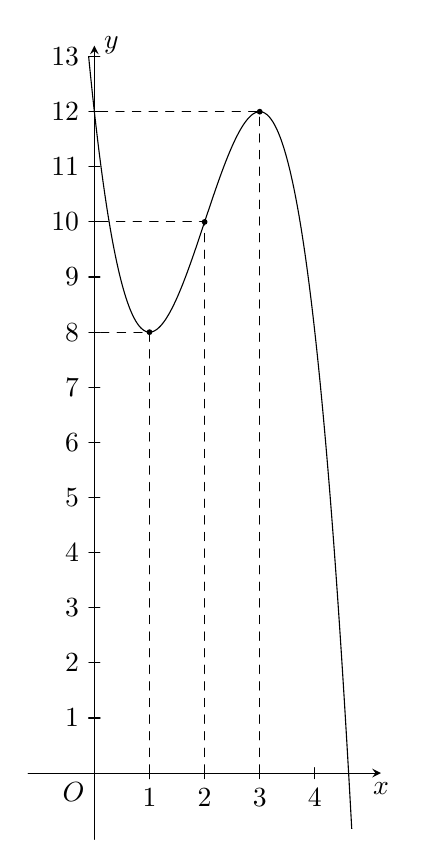
\begin{tikzpicture}[scale=0.7, line join=round, line cap=round, >=stealth]
					\tikzset{every node/.style={scale=1}}
					\def\xmin{-1}\def\xmax{5}\def\ymin{-1}\def\ymax{13}
					\draw[->] (\xmin-0.2,0)--(\xmax+0.2,0) node[below]{$x$};
					\draw[->] (0,\ymin-0.2)--(0,\ymax+0.2) node[right]{$y$};
					\draw (0,0) node[below left]{$O$};
					\foreach \x in {,1,2,3,4,}\draw (\x,0.1)--(\x,-0.1) node[below]{$\x$};
					\foreach \y in {,1,2,3,4,5,6,7,8,9,10,11,12,13}\draw (0.1,\y)--(-0.1,\y) node[left]{$\y$};
					\clip (\xmin,\ymin) rectangle (\xmax,\ymax);
					\draw[smooth,samples=200,domain=\xmin:\xmax] plot (\x,{-1*((\x)^3)+6*((\x)^2)+-9*(\x)+12});
					\draw[dashed] (2,0)--(2,10)--(0,10);\fill (2,10)circle(1.5pt);
					\draw[dashed] (1,0)--(1,8)--(0,8);\fill (1,8)circle(1.5pt);
					\draw[dashed] (3,0)--(3,12)--(0,12);\fill (3,12)circle(1.5pt);
				\end{tikzpicture}
			\end{center}
			\item Tập xác định $D=\mathbb{R}\setminus \{-1\}$.\\
			$\bullet$ Sự biến thiên.
			$y'=\dfrac{3}{(x+1)^2}>0$ với mọi $x$ khác $-1$. \\ 
			Hàm số đồng biến trên khoảng $\left(-\infty;-1\right)$ và $\left(-1;+\infty\right)$. \\ 
			Hàm số không có cực trị.\\
			Giới hạn \\ 
			$\underset{x\to +\infty}{\mathop{\lim}}y=\underset{x\to +\infty}{\mathop{\lim}}\dfrac{2x-1}{x+1}=2;\underset{x\to -\infty}{\mathop{\lim}}y=\underset{x\to -\infty}{\mathop{\lim}}\dfrac{2x-1}{x+1}=2$. \\ 
			$\underset{x\to -1^{-}}{\mathop{\lim}}y=\underset{x\to -1^{-}}{\mathop{\lim}}\dfrac{2x-1}{x+1}=+\infty;\underset{x\to -1^{+}}{\mathop{\lim}}y=\underset{x\to -1^{+}}{\mathop{\lim}}\dfrac{2x-1}{x+1}=-\infty$. \\
			Do đó, đồ thị hàm số nhận đường thẳng $x=-1$ làm tiệm cận đứng và đường thẳng $y=2$ làm tiệm cận ngang.\\
			Bảng biến thiên
			\begin{center}
				
\begin{tikzpicture}[scale=.8]
					\tikzset{double style/.append style = {draw=\tkzTabDefaultWritingColor,double=\tkzTabDefaultBackgroundColor,double distance=2pt}}
					\tikzset{h style/.style = {pattern=north west lines}}
					\tkzTabInit[nocadre=false,lgt=1.5,espcl=3.5]
					{$x$ /1, $f'(x)$ /1,$f(x)$ /2}
					{$-\infty$,$-1$,$+\infty$}
					\tkzTabLine{  ,+,d ,+ , }
					\tkzTabVar{-/$2$,+D-/$+\infty$/$-\infty$,+/$2$ }
				\end{tikzpicture}
			\end{center}
			$\bullet$ Đồ thị. \\ 
			Giao điểm của đồ thị hàm số với trục tung là $\left(0;-1 \right)$.\\
			$y=0 \Leftrightarrow \dfrac{2x-1}{x+1}=0\Leftrightarrow x=\dfrac{1}{2}$. \\ 
			Giao điểm của đồ thị hàm số với trục hoành là điểm $\left(\dfrac{1}{2};0\right)$.\\
			Đồ thị hàm số nhận $I\left(-1; 2 \right)$ làm tâm đối xứng.
			\begin{center}
				\begin{tikzpicture}[scale=0.7, line join=round, line cap=round, >=stealth]
					\tikzset{every node/.style={scale=1}}
					\def\xmin{-5}\def\xmax{3}\def\ymin{-2}\def\ymax{5}
					\draw[->] (\xmin-0.2,0)--(\xmax+0.2,0) node[below]{$x$};
					\draw[->] (0,\ymin-0.2)--(0,\ymax+0.2) node[right]{$y$};
					\draw (0,0) node[below left]{$O$};
					\foreach \x in {-5, -4,-3,-2,-1,1,2}\draw (\x,0.1)--(\x,-0.1) node[below]{$\x$};
					\foreach \y in {-1,1,2,3,4,5}\draw (0.1,\y)--(-0.1,\y) node[left]{$\y$};
					\clip (\xmin,\ymin) rectangle (\xmax,\ymax);
					\draw[dashed] (\xmin,2.0)--(\xmax,2.0);
					\draw[dashed] (-1.0,\ymin)--(-1.0,\ymax);
					\draw[smooth,samples=200,domain=\xmin:-1.1] plot (\x,{(2*(\x)+-1)/(1*(\x)+1)});
					\draw[smooth,samples=200,domain=-0.9:\xmax] plot (\x,{(2*(\x)+-1)/(1*(\x)+1)});
					\draw[dashed] (-1,0)--(-1,2)--(0,2);\fill (-1,2)circle(1.5pt);
				\end{tikzpicture}
			\end{center}
			\item Tập xác định $D=\mathbb{R}\setminus \{-1\}$. \\ 
			$\bullet$ Sự biến thiên. \\ 
			Ta có $y=\dfrac{x^2-2x}{x-1}=x-1-\dfrac{1}{x-1}$. \\ 
			$y'=\dfrac{(2x-2)(x-1)-(x^2-2x)}{(x-1)^2}=\dfrac{x^2-2x+2}{(x-1)^2}=\dfrac{(x-1)^2+1}{(x-1)^2}>0$ với mọi $x$ khác $1$. \\ 
			Do đó, hàm số đồng biến trong khoảng $\left(-\infty;1 \right)$ và $\left(1;+\infty \right)$. \\
			Hàm số không có cực trị.\\
			Giới hạn \\ 
			$\underset{x\to +\infty}{\mathop{\lim}}y=\underset{x\to +\infty}{\mathop{\lim}}\dfrac{x^2-2x}{x-1}=+\infty;\underset{x\to -\infty}{\mathop{\lim}}y=\underset{x\to -\infty}{\mathop{\lim}}\dfrac{x^2-2x}{x-1}=-\infty$. \\ 
			$\underset{x\to{1^{-}}}{\mathop{\lim}}y=\underset{x\to{1^{-}}}{\mathop{\lim}}\dfrac{x^2-2x}{x-1}=+\infty;\underset{x\to{1^{+}}}{\mathop{\lim}}y=\underset{x\to{1^{+}}}{\mathop{\lim}}\dfrac{x^2-2x}{x-1}=-\infty$. \\ 
			$\underset{x\to +\infty}{\mathop{\lim}}[y-(x-1)]=\underset{x\to +\infty}{\mathop{\lim}}\left(x-1-\dfrac{1}{x-1}-(x-1)\right)=\underset{x\to +\infty}{\mathop{\lim}}-\dfrac{1}{x-1}=0$. \\ 
			$\underset{x\to -\infty}{\mathop{\lim}}[y-(x-1)]=\underset{x\to -\infty}{\mathop{\lim}}\left(x-1-\dfrac{1}{x-1}-(x-1)\right)=\underset{x\to -\infty}{\mathop{\lim}}-\dfrac{1}{x-1}=0$. \\ 
			Do đó, đồ thị hàm số nhận đường thẳng $x=1$ làm tiệm cận đứng và đường thẳng $y=x-1$ làm tiệm cận xiên.\\
			Bảng biến thiên
			\begin{center}
				
\begin{tikzpicture}[scale=.8]
					\tikzset{double style/.append style = {draw=\tkzTabDefaultWritingColor,double=\tkzTabDefaultBackgroundColor,double distance=2pt}}
					\tikzset{h style/.style = {pattern=north west lines}}
					\tkzTabInit[nocadre=false,lgt=1.5,espcl=3.5]
					{$x$ /1, $f'(x)$ /1,$f(x)$ /2}
					{$-\infty$,$1$,$+\infty$}
					\tkzTabLine{  ,+,d ,+ , }
					\tkzTabVar{-/$-\infty$,+D-/$+\infty$/$-\infty$,+/$+\infty$ }
				\end{tikzpicture}
			\end{center}
			$\bullet$ Đồ thị. \\ 
			Giao điểm của đồ thị hàm số với trục tung là $\left(0;0 \right)$.\\
			$y=0\Leftrightarrow \dfrac{x^2-2x}{x-1}=0\Leftrightarrow \hoac{&x=0 \\&x=2}$.\\
			Đồ thị hàm số giao với $Ox$ tại các điểm $\left(0;0 \right)$ và $\left(2;0\right)$.\\
			Đồ thị hàm số nhận $I\left(1; 0 \right)$ làm tâm đối xứng.
			\begin{center}
				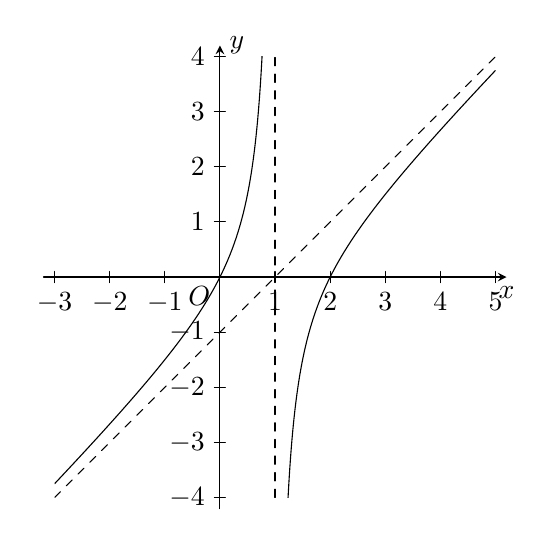
\begin{tikzpicture}[scale=0.7, line join=round, line cap=round, >=stealth]
					\tikzset{every node/.style={scale=1}}
					\def\xmin{-3}\def\xmax{5}\def\ymin{-4}\def\ymax{4}
					\draw[->] (\xmin-0.2,0)--(\xmax+0.2,0) node[below]{$x$};
					\draw[->] (0,\ymin-0.2)--(0,\ymax+0.2) node[right]{$y$};
					\draw (0,0) node[below left]{$O$};
					\foreach \x in {-3,-2,-1,1,2,3,4,5}\draw (\x,0.1)--(\x,-0.1) node[below]{$\x$};
					\foreach \y in {-4,-3,-2,-1,1,2,3,4}\draw (0.1,\y)--(-0.1,\y) node[left]{$\y$};
					\clip (\xmin,\ymin) rectangle (\xmax,\ymax);
					\draw[dashed] (1.0,\ymin)--(1.0,\ymax);
					\draw[dashed,domain=\xmin:\xmax] plot (\x,{1.0*(\x)+-1.0});
					\draw[smooth,samples=200,domain=\xmin:0.9] plot (\x,{(1*((\x)^2)+-2*(\x)+0)/(1*(\x)+-1)});
					\draw[smooth,samples=200,domain=1.1:\xmax] plot (\x,{(1*((\x)^2)+-2*(\x)+0)/(1*(\x)+-1)});
				\end{tikzpicture}
			\end{center}
		\end{enumerate}
	}
\end{bt}

% từ: cau-hoi/lop12/2D1_Ung_dung_dao_ham_de_khao_sat_ham_so/2D1-2-1_Tim_cuc_tri_cua_ham_so_cho_boi_cong_thuc.tex
\begin{bt}%[2D1H2-1]%[ma:c20b68c5]
	Tìm các khoảng đồng biến, nghịch biến  và các điểm cực trị của các hàm số sau:
	\begin{enumEX}{2}
		 \item $y=2x^3+3x^2-12x+2\,024$.
		 \item $y=x^4+2\,024$.
		\item $y=-\dfrac{1}{4}x^4+2x^2+2$. 
		\item $y=x^4-2x^2-2$. 
	\end{enumEX}
	\loigiai{ 
		\begin{enumEX}{1}
			 \item
			Ta có: $y'=6x^2+6x-12=0 \Leftrightarrow\hoac{&x=1  \\ &x=-2.}$\\
			Bảng biến  thiên:
			\begin{center}
				
\begin{tikzpicture}
					\tkzTabInit[lgt=1.2,espcl=2.5] 
						{$x$ /0.8,$f’(x)$ /0.8,$f (x)$ /2.5} 
						{$-\infty$,$-2$,$1$,$+\infty$} 
					 \tkzTabLine{,+,0,-,0,+,}
					 \tkzTabVar{-/$-\infty$,+/$2\,044$,-/$2\,017$,+/$+\infty$}
				\end{tikzpicture}
			\end{center}
			 Quan sát bảng biến thiên ta có hàm số đồng biến trên các khoảng $(-\infty;-2)$, $(1;+\infty)$ và nghịch biến trên khoảng $(-2; 1)$.\\
			Hàm số đạt cực  đại tại điểm $x=-2$, giá trị cực đại $y=2044$.\\
			Hàm số đạt  cực tiểu tại điểm $x=1$, giá trị cực tiểu $y=2017$.
			 \item Ta có tập xác định $D=\mathbb{R}$ và có đạo hàm $y'=4x^3$; $y'=0 \Leftrightarrow 4x^3=0 \Leftrightarrow x=0$.\\
			Bảng  biến thiên
			\begin{center}
				
\begin{tikzpicture}
					\tkzTabInit[lgt=1.2,espcl=3.5] 
						{$x$/0.8,$f’(x)$/0.8,$f  (x)$/2.5}
						 {$-\infty$,$0$,$+\infty$}
					 \tkzTabLine{,-,0,+,}
					 \tkzTabVar{+/$+\infty$,-/$2\,024$,+/$+\infty$}
				\end{tikzpicture}
			\end{center}
			Từ bảng biến thiên, hàm số đồng biến  trên khoảng $(0;+\infty)$ và nghịch biến trên khoảng $(-\infty; 0)$.\\
			Hàm số đạt cực tiểu tại điểm $x=0$, giá trị cực tiểu $y=2\,024$. 
			 \item Tập xác định $D=\mathbb{R}$.\\
			Đạo hàm $y'=-x^3+4x=-x(x^2-4)$; $y'=0 \Leftrightarrow-x(x^2-4)=0 \Leftrightarrow\hoac{&x=0 \\& x= \pm  2.}$\\
			Bảng  biến thiên
			\begin{center}
				
\begin{tikzpicture}
					 \tkzTabInit[lgt=1.2,espcl=2.5]
						 {$x$/0.8,$f’(x)$/0.8,$f (x)$/2.5}
						 {$-\infty$,$-2$,$0$,$2$,$+\infty$}
					\tkzTabLine{,+,0,-,0,+,0,-,} 
					\tkzTabVar{-/$-\infty$,+/$6$,-/$2$,+/$6$,-/$-\infty$} 
				\end{tikzpicture}
			\end{center}
			 Suy ra hàm số nghịch biến trên các khoảng $(-2;0)$ và $(2;+\infty)$, đồng biến trên các khoảng $(0;2)$ và $(-\infty;-2)$.\\
			Hàm số đạt cực đại tại điểm $x=  \pm 2$, giá trị cực đại $y=6$.\\
			Hàm số đạt cực tiểu tại  điểm $x=0$, giá trị cực tiểu $y=2$.
			\item Tập  xác định $D=\mathbb{R}$.\\
			Ta có $y'=4x^3-4x$, $y'=0 \Leftrightarrow  x=0, x= \pm 1$.\\
			Bảng  biến thiên
			\begin{center}
				
\begin{tikzpicture}
					\tkzTabInit[lgt=1.2,espcl=2.5] 
						{$x$/0.8,$f’(x)$/0.8,$f (x)$/2.5} 
						 {$-\infty$,$-1$,$0$,$1$,$+\infty$}
					\tkzTabLine{,-,0,+,0,-,0,+,} 
					\tkzTabVar{+/$+\infty$,-/$-3$,+/$-2$,-/$-3$,+/$+\infty$} 
				\end{tikzpicture}
			\end{center}
			Từ bảng  biến thiên ta suy ra hàm số nghịch biến trên mỗi khoảng $(-\infty;-1)$ và $(0; 1)$ và đồng biến trên các khoảng $(-1;0)$, $(1;+\infty)$.\\
			Hàm số đạt cực đại tại điểm $x=0$, giá trị  cực đại $y=-2$.\\
			Hàm số đạt cực tiểu  tại điểm $x= \pm 1$, giá trị cực tiểu $y=-3$.
		\end{enumEX}
	} 
\end{bt}

% từ: cau-hoi/lop12/2D1_Ung_dung_dao_ham_de_khao_sat_ham_so/2D1-2-2_Tim_cuc_tri_dua_vao_BBT_do_thi.tex
\begin{ex}%[2D1N2-2]%[ma:06e77e60]
	\immini{Cho hàm  số $y=ax^4+bx^3+cx^2+dx+e, (a, b,c,d,e \in \mathbb{R})$
	có đồ  thị như hình bên. Số điểm cực trị của hàm số là
	 \choice
		{$0$} 
		{$1$} 
		 {$2$}
		{\True $3$}} 
		 {
		\begin{tikzpicture}[>=stealth,scale=0.8]
			\draw[->]  (-2.5,0)--(2.5,0) node[below]{$x$};
			 \draw[->] (0,-1.5)--(0,2.2) node[left]{$y$};
			\begin{scope}
				\clip (-2.3,-2.5)  rectangle (2.3,2);
				\draw[samples=100,domain=2:-2] plot (\x,{(\x)^4-2*(\x)^2}); 
			\end{scope}
			\draw (0,0)  node[above left]{$O$};
		\end{tikzpicture}
		} 
	\loigiai{ 
		Dựa vào đồ thị hàm số ta suy ra  số điểm cực trị của hàm số là $3$.
	} 
\end{ex}

% từ: cau-hoi/lop12/2D1_Ung_dung_dao_ham_de_khao_sat_ham_so/2D1-2-2_Tim_cuc_tri_dua_vao_BBT_do_thi.tex
\begin{bt}%[2D1H2-2]%[ma:5dd4ab0c]
% nguon: Archive/2024/0. [LVH] BG - 12 New - 4in1-20240625T224301Z-001/0. [LVH] BG - 12 New - 4in1/2. [LVH] TEX SGK 12 NEW-20240418T074833Z-001/2. [LVH] TEX SGK 12 NEW/[LVH] SGK-12-KNTT/data/C1/12-SGK-KNTT-1-1.tex #1119
%[Dự án Tex hóa SKG KNTT - Nguyễn Mạnh Trung Anh]
	Đồ thị của đạo hàm bậc nhất $y=f'(x)$ của hàm số $f(x)$ được cho trong hình $1.13$.
	\begin{enumerate}
		\item Hàm số $f(x)$ đồng biến trên những khoảng nào? Giải thích.
		\item Tại giá trị nào của $x$ thì $f(x)$ có cực đại và cực tiểu? Giải thích.
	\end{enumerate}
	\begin{center}
		\begin{tikzpicture}[line join=round, line cap=round,scale=2,transform shape,scale=0.6]
			
			\def\xmin{-1} \def\xmax{9}
			\def\ymin{-2.5} \def\ymax{3} 
			\draw[->] (\xmin,0)--(\xmax,0) node [above left]{$x$};
			\draw[->] (0,\ymin)--(0,\ymax) node [below right]{$y$};
			\node at (0,0) [below left]{$O$};
			\node at (3,2.2) {$y=f'(x)$};
			\foreach \x in{1,2,3,4,5,6}\draw[fill=black] (\x,0) circle (.5pt) node[below]{\footnotesize $\x$};
			\clip (\xmin+0.1,\ymin+0.1) rectangle (\xmax-0.1,\ymax-0.1);
			\draw[line width=.5mm, red] (0,0)
			..controls +(-60:.2) and +(180:.5) ..(1,-1.2)
			..controls +(0:1) and +(180:.8) ..(3,1.7)
			..controls +(0:1.1) and +(180:1) ..(5,-2)
			..controls +(0:1) and +(180:.8) ..(6.8,1.8)
			..controls +(0:.3) and +(180:.3) ..(7.5,1.5)
			..controls +(0:.5) and +(-100:.5) ..(8.5,2.7)
			;
		\end{tikzpicture}
	\end{center}
	\loigiai{
		\begin{enumerate}
			\item Từ đồ thị hàm số, ta có $f'(x)>0\Leftrightarrow\heva{&x\in(2;4)\\&x\in(6;+\infty).}$ và liên tục trên hai khoảng đó.\\
			Do đó hàm số $f(x)$ đồng biến trên $(2;4)$ và $(6;+\infty)$.
			\item Từ đồ thị hàm số, ta có $f'(x)=0\Leftrightarrow\heva{&x=2\\&x=4\\&x=6}$ và qua các điểm đó thì $f'(x)$ đổi dấu.\\
			Vậy tại các điểm $x=2$, $x=4$, $x=6$ thì hàm số $f(x)$ có cực đại hoặc cực tiểu.
		\end{enumerate}
	}
\end{bt}

% từ: cau-hoi/lop12/2D1_Ung_dung_dao_ham_de_khao_sat_ham_so/2D1-2-2_Tim_cuc_tri_dua_vao_BBT_do_thi.tex
\begin{bt}%[2D1H2-2]%[ma:bae67ef7]
% nguon: Archive/2024/TaiLieuGiangDay/1.HamSo/1. K12 - 4in1 - Hamso/ThubaiGoc/Bai2-Dang2.tex #2621
%[BG12, Tran Tony]
	\immini{Cho hàm số $y=f(x)$ xác định trên $\mathbb{R}$ và có đồ thị hàm số $y=f'(x)$ là đường cong ở hình bên. Hỏi hàm số $y=f(x)$ có bao nhiêu điểm cực trị?
	}
	{
		\begin{tikzpicture}[scale=1, font=\footnotesize, line join=round, line cap=round, >=stealth]
			\clip (-2.5,-.5) rectangle (2.5,2.5);
			\def\xmin{-2.5} \def\xmax{2.5}
			\def\ymin{-.5} \def\ymax{2.5} 
			\draw[->] (\xmin,0)--(\xmax,0) node [above left]{\tiny $x$};
			\draw[->] (0,\ymin)--(0,\ymax) node [below right]{\tiny $y$};
			\node at (0,0) [below left]{\tiny $O$};
			\node at (1.8,1.2) [below]{\tiny $y=f'(x)$};
			\draw (-1.7,2.2)
			..controls +(-80:.3) and +(140:.2) ..(-1.3,-.3)
			..controls +(-40:.1) and +(-120:.3) ..(-1,.7)
			..controls +(60:.2) and +(-150:.2) ..(-.6,0)
			..controls +(-30:.2) and +(-140:.35) ..(.45,2.2)
			..controls +(40:.3) and +(100:.3) ..(1.2,-.4)
			;
		\end{tikzpicture}	
	}
	\loigiai{
		Số cực trị của hàm số $ y=f(x) $ là số điểm cắt của $ y=f'(x) $ với trục hoành.\\
		Dựa vào đồ thị hàm số ta thấy có ba điểm cắt và một điểm đồ thị hàm số tiếp xúc trục hoành.\\
		Vậy hàm số $ y=f(x) $ có $3$ điểm cực trị.		
	}
\end{bt}

% từ: cau-hoi/lop12/2D1_Ung_dung_dao_ham_de_khao_sat_ham_so/2D1-2-7_Toan_thuc_te_ung_dung_cuc_tri_cua_ham_so.tex
\begin{ex}%[2D1V2-7]%[ma:04ec8ac5]
% nguon: Archive/2024/TaiLieuGiangDay/1.HamSo/1. K12 - 4in1 - Hamso/ThubaiGoc/Bai2-Dang8.tex #2730
%[Bài giảng 12-4in1, Nhật Thiện]
	\immini{Một người phụ nữ đứng ở vị trí $A$ của một bờ hồ hình tròn có bán kính $2$ km. Cô ấy muốn đến điểm $C$ nằm đối diện với $A$ ở phía bên kia của hồ (tham khảo hình vẽ bên). Biết rằng vận tốc đi bộ và vận tốc chèo thuyền của cô gái này lần lượt là $4$ km/h và $2$ km/h.}{
	\begin{tikzpicture}[scale=1, font=\footnotesize, line join=round, line cap=round, >=stealth]
		\def\r{2}
		\path 
		(0,0) coordinate (O)
		(O)+(180:\r) coordinate (A)
		(O)+(0:\r) coordinate (C)
		(O)+(60:\r) coordinate (B)
		;
		\draw (O) circle (\r);
		\draw (A)--(B)--(C)--cycle;
		\draw    pic["$\alpha$", draw=black, angle eccentricity=1.2, angle radius=1cm]
		{angle=C--A--B}; %góc
		\foreach \p/\r in {A/180,C/0,B/90}
		\fill (\p) circle (1.5pt) node[shift={(\r:3mm)}]{$\p$};
	\end{tikzpicture}	
}
	\choiceTF[t]
	{Hàm số $T(\alpha)=\alpha-\cos \alpha$ với $0\le \alpha\le \dfrac{\pi}{2}$ mô tả tổng thời gian di chuyển bằng đường bộ và chèo thuyền của cô gái, với $\alpha$ là góc chèo thuyền của cô gái}
	{Thời gian đi bộ của cô gái từ $A$ đến $C$ là $1$ giờ}
	{\True Thời gian chèo thuyền của cô gái từ $A$ đến $C$ là $2$ giờ}
	{\True Khi $\alpha=\dfrac{\pi}{6}$ thì thời gian di chuyển của cô gái đạt cực trị}
	\loigiai{
		Quãng đường đi bộ của cô gái là $\ell_{BC} =2\cdot 2\alpha=4\alpha$.\\
		Thời gian đi bộ của cô gái là $t_{\text{đi bộ}}=\dfrac{4\alpha}{4}=\alpha$.\\
		Quãng đường chèo thuyền của cô gái là $AB=AC\cdot \cos \alpha=4\cdot \cos \alpha$.\\
		Thời gian chèo thuyền của cô gái là $t_{\text{chèo thuyền}}=\dfrac{4\cos \alpha}{2}=2\cos \alpha$.\\
		Tổng thời gian di chuyển là $T(\alpha)=t_{\text{đi bộ}}+t_{\text{chèo thuyền}}=\alpha+2\cos \alpha$ với $0\le \alpha\le \dfrac{\pi}{2}$.\\
		Xét $T'(\alpha)=1-2\sin \alpha=0\Leftrightarrow \sin \alpha=\dfrac{1}{2}\Leftrightarrow \alpha=\dfrac{\pi}{6}$.
		\begin{center}
			\begin{tikzpicture}
\tkzTabInit[nocadre=false,lgt=1.2,espcl=2.5,deltacl=0.6]
{$\alpha$ /0.6,$T’$ /0.6,$T$ /2}
{$0$,$\frac{\pi}{6}$,$\frac{\pi}{2}$}
\tkzTabLine{,+,0,-,}
\tkzTabVar{-/$2$,+/$2{,}6$,-/$1{,}57$}
\end{tikzpicture}
		\end{center}
	\begin{itemchoice}
	\itemch Phát biểu sai.
	\itemch Phát biểu sai.
	\itemch Phát biểu đúng.
	\itemch Phát biểu đúng.
\end{itemchoice}
}
\end{ex}

% từ: cau-hoi/lop12/2D1_Ung_dung_dao_ham_de_khao_sat_ham_so/2D1-3-1_GTLN_GTNN_tren_doan.tex
\begin{ex}%[2D1H3-1]%[ma:59e5b200]
	\immini{ 
	Cho hàm số $y=f(x)$ liên tục trên $\mathbb{R}$ và có đồ thị như hình bên. Gọi $m,M$ lần lượt là giá trị nhỏ nhất và giá trị lớn nhất của hàm số $f(x)$ trên đoạn  $[-2;2]$. Phát biểu nào sau đây là đúng?
	 \choice
		{$m=-2$,  $M=2$}
		 {$m=1$, $M=3$}
		 {$m=3$, $M=1$}
		{\True $m=-1$, $M=3$} 
		}{\resizebox{!}{5cm}{\begin{tikzpicture}[line join=round,line cap=round,>=stealth]
		\draw[->]  (-2.5,0)--(3,0) node[below]{$x$};
		\draw[->] (0,-2.0)--(0,4.5)  node[left]{$y$};
		\draw[samples=100,domain=-2.1:2.1]  plot (\x,{-(\x)^3+3*(\x)+1});
		\draw (0,0) node[below  right]{$O$};
		\draw[dashed] 
			(-1,0)  node[above]{$-1$}
			 (0,1) node[left]{$1$}
			 (0,-1) node[right]{$-1$}
			(-2,0)  node[above left]{$-2$}
			(0,3) node[above left]{$3$} 
			 (1,0) node[below right]{$1$}
			(2,0) node[below right]{$2$} 
			 (1,0)--(1,3)--(0,3)
			(-1,0)--(-1,-1)--(0,-1); 
		 \fill (2,0) circle (1pt);
		 \fill (0,1) circle (1pt);
		 \fill (1,3) circle (1pt);
		\fill (-1,-1)  circle (1pt);
		\fill (-2,0) circle (1pt); 
		\fill (0,0)  circle (1pt);
	\end{tikzpicture}
		 }
		} 
	 \loigiai{
		Dựa vào đồ thị ta thấy hàm số trên đoạn $[-2;2]$, giá trị nhỏ nhất của  hàm số $f(x)$ bằng $-1$ tại $x=-1$, giá trị lớn nhất của hàm số $f(x)$ bằng $3$ tại $x=1$.
	 }
\end{ex}

% từ: cau-hoi/lop12/2D1_Ung_dung_dao_ham_de_khao_sat_ham_so/2D1-3-1_GTLN_GTNN_tren_doan.tex
\begin{ex}%[2D1V3-1]%[ma:f6e15fdc]
	Cho hàm số $y=\left(x+m\right)^3-3\left(x+m\right)+1+n$. Biết hàm  số nghịch biến trên khoảng $\left(0;2\right)$ và giá trị lớn nhất của hàm số trên $\left[-1;1\right]$ bằng $4$. Tính $m+n$.
	 \choice
		{\True $m+n=0$} 
		 {$m+n=2$}
		{$m+n=-1$} 
		{$m+n=1$} 
	\loigiai{ 
		Ta  có: $y'=3\left(x+m\right)^2-3=3\left(x+m+1\right)\left(x+m-1\right)$.\\
		Giải phương trình  $y'=0\Leftrightarrow \hoac{&x=1-m\\&x=-1-m.}$\\
		 Bảng biến thiên.\\
		\begin{center}
			\begin{tikzpicture}
				\tkzTabInit 
					[lgt=1.5,espcl=2] 
					{$x$/1.2,$f’(x)$/1} 
					 {$-\infty$,$-m-1$,$-m+1$,$+\infty$}
				 \tkzTabLine{,+,0,-,0,+,}
			\end{tikzpicture}
		\end{center}
		Hàm số nghịch biến trên $\left(0;2\right)$  khi
		$$-m-1 \le 0 < 2\le -m+1 \Leftrightarrow \heva{& m\ge -1 \\&  m \le -1} \Leftrightarrow m=-1.$$\\
		Với $m=-1$ thì $y'=0\Leftrightarrow \hoac{&x=0\in \left[-1;1\right] \\  &x=2\notin \left[-1;1\right].}$\\
		Ta có $y(0)=n+3; \, y(1)=n+1; \, y\left(-1\right)=n-1\Rightarrow {\mathop{\max}\limits_{\left[-1;1\right]}} y=n+3=4\Rightarrow n=1$.\\ 
		Vậy $ m+n=0$. 
	 }
\end{ex}

% từ: cau-hoi/lop12/2D1_Ung_dung_dao_ham_de_khao_sat_ham_so/2D1-3-1_GTLN_GTNN_tren_doan.tex
\begin{ex}%[2D1H3-1]%[ma:c9a59cf9]
	\immini{Cho hàm số $y=f(x)$ có đạo hàm $y=f'(x)$ liên tục trên $\mathbb{R}$ và đồ thị hàm số $f'(x)$ như  hình vẽ bên.
	\choiceTF 
		{Hàm số có hai điểm  cực trị}
		{Hàm số  $y=f(x)$ đồng biến trên khoảng $\left(1;+\infty \right)$}
		{\True $f(1)  > f(2) > f(4)$}
		{\True Trên đoạn $\left[1; 4\right]$ thì giá trị lớn nhất của hàm số $f(x)$ là $f(1)$}}{\begin{tikzpicture}[line join = round,line cap = round,>=stealth,font=\footnotesize,scale=0.6]
		\def\xt{-2} \def\xp{6} \def\yd{-3}  \def\yt{4}
		 \draw[->] (\xt,0)--(\xp,0) node[below]{$x$};
		\draw[->] (0,\yd)--(0,\yt) node[left]{$y$}; 
		\fill (0,0)  circle (1.5pt) node[below left]{$O$};
		\begin{scope}
			\clip  (\xt+0.1,\yd+0.1) rectangle (\xp-0.1,\yt-0.1);
			\draw[samples=150,smooth,domain=-2:5]  plot (\x,{0.2*(\x-1)*(\x+1)*(\x-4)});
		\end{scope}
		\fill (1,0) circle  (1.5pt) node[above]{$1$}
			(4,0) circle  (1.5pt) node[below right]{$4$}
			(-1,0)  circle (1.5pt) node[above left]{$-1$};
	\end{tikzpicture}
		 }
	\loigiai{ 
		\begin{itemchoice}
			\itemch Ta có $f'(x)=0$ có ba nghiệm bội lẻ là $x=\pm  1$, $x=4$ nên hàm số $y=f(x)$ có ba điểm cực trị.
			\itemch Dựa vào đồ thị hàm số $y=f'(x)$, ta thấy hàm số $y= f(x)$ đồng biến trên hai khoảng  $(-1;1)$ và $(4; +\infty)$.
			\itemch Do hàm số nghịch biến trên đoạn $[1;4]$ mà $1<2< 4$  nên $f(1)> f(2)> f(4)$.
			\itemch Ta có hàm số nghịch biến trên $[1; a) $ và đồng biến trên $(a;  4]$ (với $a\in(1;4)$) nên $\displaystyle \max_{[1;4]} f(x)= f(4)$.
		\end{itemchoice}
	} 
\end{ex}

% từ: cau-hoi/lop12/2D1_Ung_dung_dao_ham_de_khao_sat_ham_so/2D1-3-3_Su_dung_cac_danh_gia_bat_dang_thuc_co_dien.tex
\begin{ex}%[2D1H3-3]%[ma:c914238c]
	Cho  hàm số $y=f(x)$ liên tục trên $\mathbb{R}$ và có đồ thị như hình dưới
	\begin{center}
		\begin{tikzpicture}[>=stealth]
			\draw[->] (-1.5,0) --(0,0) node[below 
				 right]{$O$} -- (4,0)
				node[below]{$x$}; 
			\draw[->](0,-3.5)--(0,1.5) 
				node[right]{$y$}; 
			 \draw[smooth,blue,line width=1]
				plot[domain=-1.05:3.05] 
				(\x,{(\x)^(3)-3*(\x)^(2)+1}); 
			\draw[dashed] (0,-3)  node[left]{} -- (2,-3) --
				 (2,0) node[above]{$2$};
			\draw (0,-3) node[above right]  {$-3$} circle (1pt);
			 \draw (2,0) circle (1pt);
			\draw (1,0)  node[above] {$1$} circle (1pt);
			\draw (0,1)  node[above left] {$1$}circle (1pt);
			\draw (3,0) node[above  right] {$3$}circle (1pt);
			\draw (-1,0)  node[above] {$-1$}circle (1pt);
		\end{tikzpicture}
	\end{center}
	Tìm giá trị lớn nhất của hàm số $y=f^2(x)+3$ trên  đoạn $[0; 2]$.
	 \choice
		{\True  $12$}
		{$13$} 
		 {$2$}
		{$9$} 
	 \loigiai{
		Đặt $g(x)=f^2(x)+3$. Từ đồ thị đã cho ta  có $\exists x_0 \in(0; 1)$ để $f\left(x_0\right)=0$.
		Với $x\in [0;2]$  thì
		\begin{eqnarray*}
			-3 \leq f(x) \leq 1 &\Rightarrow&  0 \leq f^2(x) \leq 9\\
			&\Rightarrow& 3 \leq  f^2(x)+3 \leq 12\\
			&\Rightarrow& 3 \leq g(x)  \leq 12\\
			&\Rightarrow& \max _{[0; 2]} g(x)=12  \text {khi } f(x)=-3\\
			&\Rightarrow& x=2  \in[0; 2].
		\end{eqnarray*}
	 }
\end{ex}

% từ: cau-hoi/lop12/2D1_Ung_dung_dao_ham_de_khao_sat_ham_so/2D1-3-3_Su_dung_cac_danh_gia_bat_dang_thuc_co_dien.tex
\begin{bt}%[2D1V3-3]%[ma:91a60ee4]
	Hàm số $y = (x + m)^3 + (x + n)^3 - x^3$ (tham số là $m, n$) đồng biến trên $(-\infty; +\infty)$. Biết giá trị nhỏ nhất của biểu thức $P =  4\left(m^2 + n^2\right) - 2m - 2n$ là $-\dfrac{a}{b}$, với $\dfrac{a}{b}$ là phân số tối giản. Tính $a+b$.
	\shortans{5} 
	 \loigiai{
		Ta có $y' = 3(x + m)^2 +  3(x + n)^2 - 3x^2 = 3\left[x^2 + 2(m + n)x + n^2 + m^2\right]$.\\
		Để hàm số đồng biến trên $(-\infty; +\infty)$ thì $y' \ge 0,\ \forall x \in \mathbb{R} \Leftrightarrow \Delta' = (m + n)^2  - (m^2 + n^2) \le 0 \Leftrightarrow mn \le 0$.\\
		Mặt khác,  ta có
		\begin{eqnarray*}
			P &=& 4\left(m^2 + n^2\right) - 2m - 2n = 4(m + n)^2 - 2(m + n) -  8mn\\
			&=& \left[2(m + n) - \dfrac{1}{2} \right]^2  + (-8mn) - \dfrac{1}{4} \ge -\dfrac{1}{4}.
		\end{eqnarray*}
		Suy ra $Min\,P =  -\dfrac{1}{4} \Leftrightarrow \heva{&n = 0, m = \dfrac{1}{4}\\&m = 0, n = \dfrac{1}{4}}$.\\
		Do đó $a=1$, $b=4$.  Vậy $a+b=5$.
	} 
\end{bt}

% từ: cau-hoi/lop12/2D1_Ung_dung_dao_ham_de_khao_sat_ham_so/2D1-3-6_Toan_thuc_te_ung_dung_GTLN_GTNN_cua_ham_so.tex
\begin{ex}%[2D1H3-6]%[ma:b9a71c62]
	Một vật chuyển động theo quy luật $s=\dfrac{1}{3}t^3-t^2+9t$ với $t$ (giây) là khoảng thời gian tính từ lúc vật bắt đầu chuyển động và $s$ (mét) là quãng đường đi được trong thời gian đó. Hỏi trong khoảng thời gian $10$  giây kể từ lúc bắt đầu chuyển động, tốc độ lớn nhất của vật đạt được bằng bao nhiêu?
	\choice 
		 {$109\left(\mathrm{m/s}\right)$}
		 {\True $89\left(\mathrm{m/s}\right)$}
		{$\dfrac{25}{3}\left(\mathrm{m/s}\right)$} 
		{$71\left(\mathrm{m/s}\right)$} 
	\loigiai{ 
		Vì  $s(t)=\dfrac{1}{3}t^3-t^2+9t\Rightarrow v(t)=t^2-2t+9$.\\
		Xét hàm $f(t)=t^2-2t+9\Rightarrow  f'(t)=2t-2=0$.\\
		Từ đó, $f'(t)=0$ khi $t=1$.\\ 
		Bảng biến thiên của hàm số $f(t)=t^2-2t+9$ với $0<t\leq  10$.
		\begin{center}
			\begin{tikzpicture}
				 \tkzTabInit[lgt=1.2,espcl=3.5]{$t$/0.7,$f'(t)$/0.7,$f (t)$/2.5}{$0$,$1$,$10$}
				 \tkzTabLine{,-,0,+,}
				 \tkzTabVar{+/$9$,-/$8$,+/$89$}
			\end{tikzpicture}
		\end{center}
		Dựa vào bảng biến thiên ta thấy tốc độ của vật  đạt được lớn nhất bằng $89$ (m/s).
	} 
\end{ex}

% từ: cau-hoi/lop12/2D1_Ung_dung_dao_ham_de_khao_sat_ham_so/2D1-4-1_Bai_toan_xac_dinh_cac_duong_tiem_can_cua_ham.tex
\begin{ex}%[2D1N4-1]%[ma:4e9bb61a]
	Cho hàm số $y=f(x)$ có đồ thị  như hình sau
	\begin{center}
		\begin{tikzpicture}[scale=0.5,font=\footnotesize,line join=round,line cap=round,>=stealth]
			\def \f{(-2*(\x)+2)/(1*(\x)+1)} 
			 \def \xo{-1}
			\def  \yo{-2}
			\def  \k{6}
			\draw[->] (\xo-\k-1,0)--(\xo+\k+1,0) node[below left] {$x$}; 
			\draw[->] (0,\yo-\k)--(0,\yo+\k) node[below  right] {$y$};
			 \draw (0,0) node [below right] {$O$};
			\foreach \x/\g in  {-1/-150,1/45}
			\draw[thin] (\x,2pt)--(\x,-2pt) +  (\g:5mm) node {\scriptsize $\x$};
			\foreach  \y/\g in {-2/-135,1/180,2/180}
			\draw[thin] (2pt,\y)--(-2pt,\y) +  (\g:5mm) node {\scriptsize $\y$};
			\begin{scope}
				\clip (\xo-\k,\yo-\k)  rectangle (\xo+\k,\yo+\k);
				\draw[smooth,samples=200,domain=\xo-\k:\xo-0.1,smooth,variable=\x]  plot (\x,{\f});
				\draw[smooth,samples=200,domain=\xo+0.1:\xo+\k,smooth,variable=\x] plot (\x,{\f}); 
				\draw[dashed,thin] 
					 (\xo,\yo-\k)--(\xo,\yo+\k)
					 (\xo-\k,\yo)--(\xo+\k,\yo);
			\end{scope}
			\draw (-4,-2)  node[shift={(90:3mm)}] {\scriptsize $y=-2$};
			\path (-1,0)--(-1,3) node[sloped,pos=0.8,shift={(90:3mm)}] {\scriptsize $x=-1$}; 
		\end{tikzpicture}
	\end{center}
	 Đồ thị hàm số trên có đường tiệm cận đứng là
	 \choice
		{\True  $x=-1$}
		 {$x=-2$}
		 {$y=-1$}
		{$y=-2$} 
	 \loigiai{
		Dựa vào đồ thị của hàm số, đường tiệm  cận đứng của đồ thị hàm số đã cho là $x=-1$.
	} 
\end{ex}

% từ: cau-hoi/lop12/2D1_Ung_dung_dao_ham_de_khao_sat_ham_so/2D1-5-1_Nhan_dang_do_thi.tex
\begin{ex}%[2D1N5-1]%[ma:58959e0e]
		Bảng biến thiên sau đây của hàm  số nào?
		\begin{center}
			\begin{tikzpicture}[>=stealth]
				 \tkzTabInit[nocadre=false,lgt=1,espcl=2.5,deltacl=0.5]
					 {$x$/.7,$y'$/.7,$y$/2}
					{$-\infty$,$-1$,$+\infty$} 
				\tkzTabLine{,+,d,+,} 
				 \tkzTabVar{-/$2$,+D-/$+\infty$/$-\infty$,+/$2$}
			\end{tikzpicture}
		\end{center}
	\choice 
			{$y=\dfrac{2x+3}{x+1}$} 
			{$y=\dfrac{2x-1}{x-1}$} 
			{\True  $y=\dfrac{2x-1}{x+1}$}
			{$y=\dfrac{x+1}{2x-1}$} 
	\loigiai{ 
			Gọi hàm số cần tìm có  dạng $y=\dfrac{ax+b}{cx+d}$ có đồ thị $(C)$.\\
			Dựa vào bảng biến thiên, ta  thấy đồ thị $(C)$ có
			\begin{itemize}
				\item Tiệm cận ngang $y=\dfrac{a}{c}=2$. 
				\item Tiệm cận đứng  $x=\dfrac{-d}{c}=-1$.
				\item Hàm số đồng biến trên từng khoảng xác định nên $ad-bc>0$. 
			\end{itemize}
			Vậy hàm số  thỏa mãn là $y=\dfrac{2x-1}{x+1}$.
		} 
	\end{ex}

% từ: cau-hoi/lop12/2D1_Ung_dung_dao_ham_de_khao_sat_ham_so/2D1-5-1_Nhan_dang_do_thi.tex
\begin{ex}%[2D1H5-1]%[ma:8dcfb462]
		Hàm số nào sau  đây có bảng biến thiên như hình dưới đây?
		\begin{center}
			\begin{tikzpicture}
				 \tkzTabInit[nocadre=false,lgt=1.2,espcl=2.5,deltacl=0.6]
					 {$x$/0.6,$y'$/0.6,$y$/2}
					{$-\infty$,$2$,$+\infty$} 
				\tkzTabLine{,-,d,-} 
				 \tkzTabVar{+/$2$,-D+/$-\infty$ / $+\infty$,-/$2$}
			\end{tikzpicture}
		\end{center}
	 \choice
			{$y  = \dfrac{2x - 7}{x - 2}$}
			{$y = \dfrac{2x + 1}{x +  2}$}
			 {\True $y = \dfrac{2x + 1}{x - 2}$}
			 {$y = \dfrac{1 - 2x}{x - 2}$}
	\loigiai{ 
			Ta có $y  = \dfrac{2x + 1}{x - 2}$.\\
			Ta có $\lim\limits_{x \to +\infty} \dfrac{2x + 1}{x - 2} = 2$,$\lim\limits_{x \to -\infty} \dfrac{2x + 1}{x - 2} = 2$, $\lim\limits_{x \to 2^+} y = +  \infty$, $\lim\limits_{x \to 2^-} y = - \infty$.\\
			Lại có $y' = \dfrac{-5}{(x - 2)^2} <  0\ \forall x\ne 2$ nên hàm số nghịch biến trên các khoảng $(-\infty;2)$ và $(2;+\infty)$.
		 }
	\end{ex}

% từ: cau-hoi/lop12/2D1_Ung_dung_dao_ham_de_khao_sat_ham_so/2D1-5-1_Nhan_dang_do_thi.tex
\begin{bt}%[2D1H5-1]%[ma:f012ca7d]
% nguon: Archive/2024/TaiLieuGiangDay/1.HamSo/1. K12 - 4in1 - Hamso/ThubaiGoc/Bai5-Dang2.tex #2121
%[Dự án Bài Giảng 12 Nhóm Toán & LaTex, Lê Minh Thiện Anh] 
	Cho hàm số $y=\dfrac{2x+1}{x-1}$.
	\begin{enumerate}
		\item Khảo sát và vẽ đồ thị của hàm số.
		\item Gọi $A$ là giao điểm của đồ thị hàm số với trục $Oy$, $I$ là giao điểm của hai đường tiệm cận của đồ thị hàm số. Tìm điểm $B$ đối xứng với $A$ qua $I$. Chứng minh rằng điểm $B$ cũng thuộc đồ thị hàm số này.
	\end{enumerate}
	\loigiai{
		\begin{enumerate}
			\item Khảo sát và vẽ đồ thị của hàm số
			\begin{itemize}
			\item Tập xác định $\mathscr{D}=\mathbb{R}\setminus \{1\}$.
			\item Sự biến thiên\\
				Đạo hàm $y'=-\dfrac{3}{(x-1)^2}$. Vì $y'<0$ với mọi $x\neq 1$ nên hàm số nghịch biến trên mỗi khoảng $(-\infty;1)$ và $(1;+\infty)$.\\
			Ta có $\lim\limits_{x\to -\infty} y=\lim\limits_{x\to -\infty} \dfrac{2x+1}{x-1}=2$; $\lim\limits_{x\to +\infty} y=\lim\limits_{x\to +\infty} \dfrac{2x+1}{x-1}=2$.\\
				$\Rightarrow$ Đường thẳng $y=2$ là tiệm cận ngang của đồ thị hàm số.\\
				Lại có $\lim\limits_{x\to 1^{-}} y=\lim\limits_{x\to 1^{-}} \dfrac{2x+1}{x-1}=-\infty$; $\lim\limits_{x\to 1^{+}} y=\lim\limits_{x\to 1^{+}} \dfrac{2x+1}{x-1}=+\infty$.\\
				$\Rightarrow$ Đường thẳng $x=1$ là tiệm cận đứng của đồ thị hàm số.\\
				Bảng biến thiên
				\begin{center}
			\begin{tikzpicture}
					\tkzTabInit[nocadre=false,lgt=1.2,espcl=4,deltacl=0.6]
					{$x$ /0.6,$y'$ /0.6,$y$ /2}
					{$-\infty$,$1$,$+\infty$}
					\tkzTabLine{,-,d,-,}
					\tkzTabVar{+/$2$,-D+/$-\infty$/$+\infty$,-/$2$}
				\end{tikzpicture}
			\end{center}
			\item Đồ thị
				\immini{
					Đồ thị của hàm số giao với trục $Ox$ tại điểm $\left(-\dfrac{1}{2};0\right)$, giao với trục $Oy$ tại điểm $(0;-1)$.\\
					Đồ thị của hàm số đã cho được biểu diễn như hình bên. Đồ thị của hàm số có tâm đối xứng là điểm $I(1;2)$.
					}{
				\begin{tikzpicture}[scale=0.7, font=\footnotesize, line join=round, line cap=round, >=stealth]
					\def\a{2} \def\b{1} \def\c{1} \def\d{-1} % Hệ số
					\def\xt{-3} \def\xp{5} \def\yt{6} \def\yd{-2} % x_trái, x_phải, y_trên, y_dưới (giới hạn)
					\draw[->] (\xt,0)--(\xp,0) node [below]{$x$};
					\draw[->] (0,\yd)--(0,\yt) node [left]{$y$};
					\node at (0,0) [below right]{$O$};
					\clip (\xt+0.1,\yd+0.1) rectangle (\xp-0.1,\yt-0.1);
					\draw[thick,red,smooth,samples=300,domain=\xt:(-\d/\c-0.1)] plot(\x,{(\a*(\x)+\b)/(\c*(\x)+\d)});
					\draw[thick,red,smooth,samples=300,domain=(-\d/\c+0.1:\xp)] plot(\x,{(\a*(\x)+\b)/(\c*(\x)+\d)});
					\draw[dashed] (-\d/\c,\yd)--(-\d/\c,\yt);
					\draw[dashed] (\xt,\a/\c)--(\xp,\a/\c);
					\fill (1,2) circle (1.5pt) node[below right]{$I$};
					\fill (0,-1) circle (1.5pt) node[left]{$-1$};
					\fill (-0.5,0) circle (1.5pt) node[above]{$-\frac{1}{2}$};
					\foreach \x in {-2,-1,1,2,3,4}
					\draw[shift={(\x,0)},color=black] (0pt,2pt) -- (0pt,-2pt);
				\foreach \y in {-1,1,2,3,4,5}
					\draw[shift={(0,\y)},color=black] (2pt,0pt) -- (-2pt,0pt);
					\node at (4.2,2) [below]{$y=2$};
					\node at (1,-1.5) [right]{$x=1$};
				\end{tikzpicture}
			}
			\end{itemize}
			\item Ta có $A(0;-1)$ và $I(1;2)$.\\
				Do điểm $B$ đối xứng với $A$ qua $I$ nên $I$ là trung điểm của đoạn $AB$ $\Rightarrow B(2;5)$.\\
				Thay tọa độ $B$ vào đồ thị hàm số $y=\dfrac{2x+1}{x-1}$ ta có $5=\dfrac{2\cdot 2+1}{2-1} \Leftrightarrow 5=5$ (đúng).\\
				Vậy điểm $B$ cũng thuộc đồ thị hàm số đã cho.
		\end{enumerate}
		}
\end{bt}

% từ: cau-hoi/lop12/2D1_Ung_dung_dao_ham_de_khao_sat_ham_so/2D1-5-2_Cac_phep_bien_doi_do_thi.tex
\begin{bt}%[2D1H5-2]%[ma:82346016]
% nguon: Archive/2024/TaiLieuGiangDay/1.HamSo/1. K12 - 4in1 - Hamso/ThubaiGoc/Bai5-Dang5.tex #2315

	Cho hàm số $y=f(x)=x^3+2x^2+x-1$. Hãy xác định khoảng biến thiên của hàm số $y=f(-x)$.
	
	\loigiai{
		Ta có, $y=f(x)=x^3+2x^2+x-1 \Rightarrow f(-x)=(-x)^3+2(-x)^2+(-x)-1=-x^3+2x^2-x-1$.\\
		$y'=f'(-x)=0\Leftrightarrow -3x^2+4x-1=0 \Leftrightarrow \hoac{&x=\dfrac{1}{3}\\&x=1.}$\\
		Khi đó ta có bảng biến thiên
		\begin{center}
			\begin{tikzpicture}[>=stealth,line join=round,line cap=round,font=\footnotesize,scale=1]
				\tkzTabInit[nocadre=false,lgt=1.2,espcl=3,deltacl=.55]
				{$x$/0.7, $y'$/0.7, $y$/1.8}
				{$-\infty$,$\dfrac{1}{3}$,$1$,$+\infty$}
				\tkzTabLine{,-,$0$,+,$0$,-,}
				\tkzTabVar{+/$\infty$,-/$f\left(\dfrac{1}{3}\right)$,+/$f(1)$,-/$-\infty$}	
			\end{tikzpicture}
			
		\end{center}
		
		Vậy hàm số đồng biến trên khoảng $\left(\dfrac{1}{3};1\right)$; nghịch biến trên khoảng $\left(-\infty;\dfrac{1}{3}\right)$ và $\left(1;+\infty\right)$.}
\end{bt}

% từ: cau-hoi/lop12/2D1_Ung_dung_dao_ham_de_khao_sat_ham_so/2D1-5-3_Bien_luan_so_giao_diem_dua_vao_do_thi_bang_bi.tex
\begin{ex}%[2D1N5-3]%[ma:331a56c6]
		Cho hàm số  $y=f(x)$ có bảng biến thiên như sau:
		\begin{center}
			\begin{tikzpicture}
				 \tkzTabInit[nocadre,espcl=2.5,lgt=1.5]
					{$x$/0.7,$f'(x)$/0.7,$f (x)$/2.1} 
					 {$-\infty$,$1$,$3$,$+\infty$}
				 \tkzTabLine{,-,0,+,0,-,}
				 \tkzTabVar{+/$+\infty$,-/$-1$,+/$3$,-/$-\infty$}
			\end{tikzpicture}
		\end{center}
		 Số nghiệm của phương trình $3f(x)+1=0$ là
	\choice 
			{$0$} 
			 {$1$}
			 {$2$}
			 {\True $3$}
	 \loigiai{
			Ta  có $3f(x)+1=0$ $\Leftrightarrow $ $f(x)=\dfrac{-1}{3}$.\\
		Vì đường thẳng $y=\dfrac{-1}{3}$ cắt đồ thị hàm  số $y=f(x)$ tại ba điểm phân biệt nên phương trình $3f(x)+1=0$ có ba nghiệm phân biệt.}
	\end{ex}

% từ: cau-hoi/lop12/2D1_Ung_dung_dao_ham_de_khao_sat_ham_so/2D1-5-3_Bien_luan_so_giao_diem_dua_vao_do_thi_bang_bi.tex
\begin{bt}%[2D1N5-3]%[ma:53559c2e]
% nguon: Archive/2024/TaiLieuGiangDay/1.HamSo/1. K12 - 4in1 - Hamso/ThubaiGoc/Bai5-Dang6.tex #2214

	Cho hàm số $y=f(x)$ xác định trên $\mathbb{R}\setminus\{2\}$, liên tục trên mỗi khoảng xác định và có bảng biến thiên như hình vẽ sau. Tìm tập hợp tất cả các giá trị của tham số thực $m$ sao cho phương trình  $f(x)=m$ có ba nghiệm phân biệt.
	\begin{center}
		\begin{tikzpicture}[>=stealth]
			\tkzTabInit[lgt=1.2,espcl=3]
			{$x$ /1,$y'$ /1,$y$ /2.5}
			{$-\infty$,$2$,$3$,$+\infty$}
			\tkzTabLine{t,-,d,+,z,-,}%
			\tkzTabVar{+/ $+\infty$ , -D-/$2$ /$-\infty$, +/ $3$, -/ $-\infty$}
		\end{tikzpicture}
	\end{center}
	\loigiai{
		Phương trình $f(x)=m$ có $3$ nghiệm phân biệt khi và chỉ khi đồ thị $y=f(x)$ và đường thẳng $y=m$ cắt nhau tại $3$ điểm phân biệt.\\
		Dựa vào bảng biến thiên ta thấy điều này tương đương với $2<m<3$.}
\end{bt}

% từ: cau-hoi/lop12/2D1_Ung_dung_dao_ham_de_khao_sat_ham_so/2D1-5-4_Su_tuong_giao_cua_hai_do_thi_lien_quan_den_to.tex
\begin{ex}%[2D1H5-4]%[ma:8165844a]
	Cho  hàm số $y=x-\dfrac{1}{x+1}$.
	\choiceTF 
		{Đồ thị của hàm số có tiệm cận đứng là $x=1$} 
		{\True Đồ thị hàm số cắt trục $Oy$ tại $M$. Phương trình tiếp tuyến  của $(C)$ tại $M$ là $y=2x-1$}
		{Tồn  tại hai tiếp tuyến của đồ thị vuông góc với nhau}
		{\True Nếu  đường thẳng $y=k$ cắt $(C)$ tại hai điểm phân biệt $A$ và $B$ sao cho $OA\perp OB$ thì $k$ là nghiệm của phương trình $k^2-k-1=0$}
	 \loigiai{
		\begin{itemchoice}
			\itemch $y=x-\dfrac{1}{x+1}$. Tập xác định $\mathbb{D}=\mathbb{R}\setminus\{-1\}$.\\ 
			Đạo hàm $y'=1+\dfrac{1}{(x+1)^2}>0,\forall x\in \mathbb{D}$ do đó hàm số luôn luôn đồng biến, không có cực đại,  cực tiểu.\\
			$\lim\limits_{x\to-1^\pm}y=\pm\infty$ nên đường thẳng $x=-1$  là tiệm cận đứng.\\
			$\lim\limits_{x\to\pm\infty}y=x$ nên đường thẳng $y=x$  là tiệm cận xiên.\\
			Bảng biến thiên 
			\begin{center}\begin{tikzpicture}[>=stealth]
		 \tkzTabInit[nocadre=false,lgt=1,espcl=2,deltacl=0.5]{$x$/.7,$y'$/.7,$y$/2}
			 {$-\infty$,$1-\sqrt{2}$,$1$,$1+\sqrt{2}$,$+\infty$}
		\tkzTabLine{,-,$0$,+,d,+,$0$,-,} 
		\tkzTabVar{+/$+\infty$,-/$4$,+D-/$+\infty$/$-\infty$,+/$-4$,-/$-\infty$} 
	\end{tikzpicture}
			\end{center}
			\itemch $M(0;-1), y'(0)=2$. Phương trình tiếp tuyến $(T)$  tại $M$ là $y=2(x-0)-1\Leftrightarrow y=2x-1$.
			\itemch Tiếp  tuyến $(T_1)$ của $(C)$ tại $P(x_1; y_1)$ có hệ số góc $k_1=y'(x_1)=1+\dfrac{1}{(x_1+1)^2}>0$.\\
			Tiếp tuyến $(T_2)$ của $(C)$ tại $Q(x_2; y_2)$ có  hệ số góc $k_2=y'(x_2)=1+\dfrac{1}{(x_2+1)^2}>0$.\\
			Do $y'(x_1)>0$, $y'(x_2)>0$ nên không  thể có 2 tiếp tuyến của $(C)$ vuông góc nhau.
			\itemch $y=x-\dfrac{1}{x+1}=\dfrac{x^2+x-1}{x+1}$.\\ 
			 Phương trình hoành độ giao điểm của $(C)$ và đường thẳng $y=k$.\\
			$\dfrac{x^2+x-1}{x+1}=k\Leftrightarrow\heva{&x \ne -1  \\&x^2 - (k-1)x - (k+1) = 0 \quad (*)}$.\\
			 Phương trình $(*)$ có 2 nghiệm phân biệt $x_A, x_B\neq-1$ và
			$\heva{&x_A + x_B=k-1\\&x_A\cdot x_B=-(k+1)}$ và $A(x_A;k)$,  $B(x_B;k)$.\\
			 Ta có $\overrightarrow{OA}=(x_A,k)$, $\overrightarrow{OB}=(x_B,k)$.\\
			$\overrightarrow{OA} \perp \overrightarrow{OB} \Leftrightarrow \overrightarrow{OA} \cdot \overrightarrow{OB} = 0 \Leftrightarrow x_A x_B + k^2  = 0 \Leftrightarrow -k - 1 + k^2 = 0 \Leftrightarrow
			\hoac{&k=\dfrac{1-\sqrt{5}}{2}\\&k=\dfrac{1+\sqrt{5}}{2}.}$\\ 
			Thử lại,  $k=\dfrac{1-\sqrt{5}}{2}$ và $k=\dfrac{1+\sqrt{5}}{2}$ đều thỏa mãn yêu cầu bài toán.
		\end{itemchoice}
	} 
\end{ex}

% từ: cau-hoi/lop12/2D1_Ung_dung_dao_ham_de_khao_sat_ham_so/2D1-5-4_Su_tuong_giao_cua_hai_do_thi_lien_quan_den_to.tex
\begin{ex}%[2D1V5-4]%[ma:e0b4e875]
	Cho hàm số $f(x)=\dfrac{2x-1}{x^2+2}$. 
	\choiceTF 
		{\True Đồ thị hàm số $y=f(x)$ nhận trục hoành làm tiệm cận ngang} 
		{Hàm số $f(x)$ có $x=2$ là điểm cực tiểu} 
		{\True Với mọi $x \in \mathbb{R}$, ta luôn có $-1 \leq f(x) \leq \dfrac{1}{2}$} 
		{Nếu $-1<m \leq 0$ thì phương trình  $f(x)=m$ có hai nghiệm}
	 \loigiai{
		\begin{itemchoice}
			 \itemch
			\begin{itemize}
				\item  Tập xác định $\mathscr{D}=\mathbb{R}$.
				\item Ta có $\lim\limits_{x\to-\infty}f(x)=0$, $\lim\limits_{x\to+\infty}f(x)=0$ suy ra $y=0$ là tiệm cận ngang của đồ thị hàm số $f(x)$ hay đồ thị hàm  số $y=f(x)$ nhận trục hoành làm tiệm cận ngang.
				 \item $f'(x)=\dfrac{-2\left(x^2-x-2\right)}{\left(x^2+2\right)^2}$;\\
				$f'(x)=0\Leftrightarrow -2\left(x^2-x-2\right)=0 \Leftrightarrow \hoac{& x=-1 \\ &  x=2.}$
				 \item Bảng biến thiên
				\begin{center}
					\begin{tikzpicture}
						\tkzTabInit[espcl=3.2,lgt=1.5,nocadre] 
						 {$x$/0.7,$f'(x)$/0.7,$f (x)$/2.1}
						{$-\infty$,$-1$,$2$,$+\infty$} 
						 \tkzTabLine{,-,0,+,0,-,}
						\tkzTabVar{+/$0$,-/$-1$,+/$\dfrac{1}{2}$,-/$0$} 
					\end{tikzpicture}
				\end{center}
			\end{itemize}
			\itemch Hàm số $f(x)$ có $x=2$  là điểm cực đại.
			\itemch Dựa vào bảng  biến thiên ta có $-1 \leq f(x) \leq \dfrac{1}{2}$ với mọi $x \in \mathbb{R}$.
			\itemch Khi $m=0$, phương trình $f(x)=m \Leftrightarrow \dfrac{2x-1}{x^2+2} =0 \Leftrightarrow 2x-1=0\Leftrightarrow  x=\dfrac{1}{2}$ chỉ có một nghiệm.
		\end{itemchoice}
	 }
\end{ex}

% từ: cau-hoi/lop12/2D1_Ung_dung_dao_ham_de_khao_sat_ham_so/2D1-5-7_Diem_dac_biet_cua_do_thi_ham_so.tex
\begin{ex}%[2D1V5-7]%[ma:708bb749]
	Cho hàm số $y=\dfrac{-x^2+2(m+1)x-m-5}{x-1}$ có đồ thị $(C)$ với $m$ là tham số 
	\choiceTF 
		 {\True Khi $m=0$ thì đồ thị hàm số có tiệm cận xiên là $y=-x+1$}
		{\True Khi $m=0$ thì  đồ thị hàm số không cắt $Ox$}
		{Để hàm số có cực đại  và cực tiểu thì $m>4$}
		{\True Khi $m=0$, tồn tại $1$  điểm $M$ thuộc đồ thị $(C)$ sao cho $x_M>1$ và độ dài $IM$ ngắn nhất ($I$ là tâm đối xứng của $(C)$). Khi đó tung độ $y_M<-4$}
	 \loigiai{
		\begin{itemchoice}
			\itemch 
			Khi $m=0$  ta có $y=\dfrac{-x^2+2x-5}{x-1}=-x+1-\dfrac{4}{x-1}$.\\
			Tập xác  định $\mathbb{D}=\mathbb{R}\setminus\{1\}$.\\
			$\lim\limits_{x\to\pm\infty}y-(-x+1) = 0$ nên $y=-x+1$ là tiệm cận  xiên.\\
			\itemch Khi $m=0$ ta  có $y=\dfrac{-x^2+2x-5}{x-1}=-x+1-\dfrac{4}{x-1}$.
			Tập xác định  $\mathbb{D}=\mathbb{R}\setminus\{1\}$.\\
			Đạo hàm  $y'=\dfrac{-x^2+2x+3}{(x-1)^2}= 0 \Leftrightarrow -x^2+2x+3=0\Leftrightarrow
			 \heva{&x=-1\Rightarrow y=4.\\&x=3 \Rightarrow y=-4.}$
			Ta có $\lim\limits_{x\to 1^\pm}y=\pm\infty$ nên $x=1$ là đường tiệm cận  đứng;\\
			$\lim\limits_{x\to\pm\infty}y-(-x+1)  = 0$ nên $y=-x+1$ là tiệm cận xiên.
			Đồ thị hàm số không cắt  $Ox$.
			\itemch $y=\dfrac{-x^2+2(m+1)x-m-5}{x-1}$;\\ $y'=\dfrac{-x^2+2x-2m-2+m+5}{(x-1)^2}=\dfrac{-x^2+2x-m+3}{(x-1)^2}$.\\ 
			Hàm số $y$ có cực đại cực tiểu khi  phương trình $-x^2+2x-m+3=0$ có hai nghiệm phân biệt $\Rightarrow\triangle'=1-m+3=4-m>0\Rightarrow m<4$.
			Nghiệm $x=1$ không phải là nghiệm của phương trình  $y'=0\Rightarrow-1+2-m+3\ne 0\Rightarrow m\ne 4$
			Điều kiện sau cùng  $m<4$.
			\itemch $x_M>1\Rightarrow  M$ thuộc nhánh bên phải của $(C)$ và $I$ là tâm đối xứng của $(C)$ nên $I(1;0)$.
			 Toạ độ điểm $M\left(a;-a+1-\dfrac{4}{a-1}\right)$;\\
			 $IM^2=(a-1)^2+\left[(-a+1)^2+\dfrac{16}{(a-1)^2}+8\right]=2(a-1)^2+\dfrac{16}{(a-1)^2}+8$\\
			$IM^2\geq  2\sqrt{2(a-1).\dfrac{16}{(a-1)}}+8\Rightarrow IM^2\ge 8(\sqrt{2}+1)\Rightarrow IM\ge\sqrt{8(\sqrt{2}+1)}$\\
			IM  ngắn nhất khi $$2(a-1)^2=\dfrac{16}{(a-1)^2}\Leftrightarrow(a-1)^4=8\Leftrightarrow a=1+\sqrt[4]8\Rightarrow y_M=-\sqrt[4]8-\dfrac{4}{\sqrt[4]8}<-4.$$
		\end{itemchoice}
	} 
\end{ex}

% từ: cau-hoi/lop12/2D4_Cac_so_dac_trung_ghep_nhom/2D4-1-1_Cong_thuc_ly_thuyet.tex
\begin{ex}%[2D4N1-1]%[ma:090d6bfd]
	Trong  các khẳng định sau, khẳng định nào \textbf{sai}?
	 \choice
		 {$\displaystyle\int 0 \mathrm{\,d}x=C$}
		 {$\displaystyle\int \dfrac{1}{x} \mathrm{\,d}x=\ln |x|+C$}
		{\True  $\displaystyle\int x^a\mathrm{\,d}x=\dfrac{x^{a+1}}{a+1}+C$}
		{$\displaystyle\int  \mathrm{\,d}x=x+C$}
	\loigiai{$\displaystyle\int x^a \mathrm{\,d}x=\dfrac{x^{a+1}}{a+1}+C$ không  đúng với trường hợp $a=-1$.}
\end{ex}

% từ: cau-hoi/lop12/2D4_Nguyen_ham_tich_phan/2D4-1-2_Nguyen_ham_co_ban_da_thuc_phan_thuc.tex
\begin{ex}%[2D4N1-2]%[ma:84b8a7c0]
	Khẳng định nào sau đây {\bf{sai}}? 
	\choice 
		{$\displaystyle\int 0\mathrm{\,d}x=C$} 
		{$\displaystyle\int x^4\mathrm{\,d}x=\dfrac{x^5}{5}+C$} 
		 {\True $\displaystyle\int \dfrac{1}{x} \mathrm{\,d}x=\ln x+C$}
		{$\displaystyle\int \mathrm{e}^x \mathrm{\,d}x=\mathrm{e}^x+C$} 
	\loigiai{ 
		Ta có  $\displaystyle\int \dfrac{1}{x} \mathrm{\,d}x=\ln|x|+C$.
	 }
\end{ex}

% từ: cau-hoi/lop12/2D4_Nguyen_ham_tich_phan/2D4-1-2_Nguyen_ham_co_ban_da_thuc_phan_thuc.tex
\begin{ex}%[2D4H1-2]%[ma:9854f712]
	Cho hàm số $F(x)=\displaystyle\int  \left(2x+\sqrt{x}\right)\mathrm{\,d}x$ (với $x>0$). Khi đó
	\choiceTF 
		 {\True $F(x)=2\displaystyle\int x\mathrm{\,d}x+\displaystyle\int \sqrt{x}\mathrm{\,d}x+C$ với $C\in \mathbb{R}$}
		 {\True $G(x)=F(x)+2024 \Rightarrow G(x)=\displaystyle\int \left(2x+\sqrt{x}\right)\mathrm{\,d}x$}
		{$F(x)=x+\dfrac{2}{3}x\sqrt{x}+C$} 
		{$F(1)=\dfrac{2}{3} \Rightarrow  F(4)=\dfrac{28}{3}$}
	 \loigiai{
		\begin{itemchoice}
			\itemch Vì  $\displaystyle\int kf(x)\mathrm{\,d}x = k\displaystyle\int f(x)\mathrm{\,d}x$, $k\ne 0$; $\displaystyle\int \left(f(x)+g(x)\right)\mathrm{\,d}x = \displaystyle\int f(x)\mathrm{\,d}x + \displaystyle\int g(x)\mathrm{\,d}x$.
			\itemch Ta có $F(x)$, $G(x)$ là  nguyên hàm của hàm số $f(x)$ thì $F(x)=G(x)+C$.
			\itemch Ta có $F(x)=\displaystyle\int \left(2x+\sqrt{x}\right)\mathrm{\,d}x = \displaystyle\int \left(2x+x^{\frac{1}{2}}\right)\mathrm{\,d}x = x^2+\dfrac{2}{3}x\sqrt{x}+C$ suy ra khẳng định sai. 
			\itemch Ta có $F(1)=1+\dfrac{2}{3}+C=\dfrac{2}{3} \Rightarrow C=-1 \Rightarrow F(x)=x^2+\dfrac{2}{3}x\sqrt{x}-1 \Rightarrow  F(4)=\dfrac{25}{3}$.
		\end{itemchoice}
	} 
\end{ex}

% từ: cau-hoi/lop12/2D4_Nguyen_ham_tich_phan/2D4-1-2_Nguyen_ham_co_ban_da_thuc_phan_thuc.tex
\begin{bt}%[2D4H1-2]%[ma:a945c437]
% nguon: Archive/2024/0. [LVH] BG - 12 New - 4in1-20240625T224301Z-001/0. [LVH] BG - 12 New - 4in1/2. [LVH] TEX SGK 12 NEW-20240418T074833Z-001/2. [LVH] TEX SGK 12 NEW/[LVH] SGK-12-KNTT/data/C4/12-c4-Bai11-nguyenham.tex #1158
 
	Tìm:
	\begin{enumerate}[a)]
		\item $\displaystyle\int\left (3\sqrt{x}+\dfrac{1}{\sqrt[3]{x}}\right )\mathrm{\,d}x$;
		\item $\displaystyle\int\sqrt{x}(7x^2-3)\mathrm{\,d}x$ ($x>0$);
		\item $\displaystyle\int \dfrac{(2x+1)^2}{x^2}\mathrm{\,d}x$;
		\item $\displaystyle\int \left (2^x + \dfrac{3}{x^2}\right )\mathrm{\,d}x$.
	\end{enumerate}
\loigiai{
\begin{enumerate}[a)]
	\item $\displaystyle\int\left (3\sqrt{x}+\dfrac{1}{\sqrt[3]{x}}\right )\mathrm{\,d}x = \int \left( 3x^{1/2} + x^{-1/3}\right)  \mathrm{\,d}x = \frac{6}{3}x^{3/2} + \dfrac{3}{2}x^{2/3} + C = 2x^{3/2} + \dfrac{3}{2}x^{2/3} + C.$
	
	\item $\displaystyle\int\sqrt{x}(7x^2-3)\mathrm{\,d}x = \int 7x^{5/2} - 3x^{1/2} \mathrm{\,d}x = \frac{14}{7}x^{7/2} - 2x^{3/2} + C = 2x^{7/2} - 2x^{3/2} + C.$
	
	\item $\displaystyle\int \dfrac{(2x+1)^2}{x^2}\mathrm{\,d}x = \int \frac{4x^2 + 4x + 1}{x^2} \mathrm{\,d}x = \int \left (4 + \frac{4}{x} + \frac{1}{x^2}\right ) \mathrm{\,d}x = 4x - 4\ln|x| - \frac{1}{x} + C.$
	
	\item $\displaystyle\int \left (2^x + \dfrac{3}{x^2}\right )\mathrm{\,d}x = \int 2^x \mathrm{\,d}x + \int \frac{3}{x^2} \mathrm{\,d}x = \frac{2^x}{\ln 2} - \frac{3}{x} + C.$
\end{enumerate}

}
\end{bt}

% từ: cau-hoi/lop12/2D4_Nguyen_ham_tich_phan/2D4-1-3_Nguyen_ham_co_ban_ham_luong_giac.tex
\begin{ex}%[2D4H1-3]%[ma:1a73e98d]
	Cho hàm số $f(x)=\left(\sin{\dfrac{x}{2}}+\cos{\dfrac{x}{2}}\right)^2$. 
	 \choiceTF
		{\True  $f(x)=1+\sin{x}$}
		{\True $f(x)$ liên  tục trên $\mathbb{R}$}
		{$\displaystyle\int f(x)\mathrm{\,d}x=\displaystyle\int\mathrm{\,d}x+\displaystyle\int  (-\cos{x})\mathrm{\,d}x$}
		{$\displaystyle\int f(x)\mathrm{\,d}x=x+\cos{x}+C$} 
	 \loigiai{
		\begin{itemchoice}
			\itemch  \textbf{Đúng}.\\
			Ta  có
			\begin{align*}
				 f(x)=&\, \left(\sin{\dfrac{x}{2}}+\cos{\dfrac{x}{2}}\right)^2\\
				=&\,  \sin^2{\dfrac{x}{2}}+2\sin{\dfrac{x}{2}}\cos{\dfrac{x}{2}}+\cos^2{\dfrac{x}{2}}\\
				=&\, \sin^2{\dfrac{x}{2}}+\cos^2{\dfrac{x}{2}}+\sin{\left(2\cdot\dfrac{x}{2}\right)}\\ 
				 =&\, 1+\sin{x}.
			\end{align*}
			 \itemch \textbf{Đúng}.\\
			Hàm số $f(x)=1+\sin{x}$ là hàm số liên tục trên  $\mathbb{R}$.
			 \itemch \textbf{Sai}.\\
			Ta có $\displaystyle\int  f(x)\mathrm{\,d}x=\displaystyle\int (1+\sin{x})\mathrm{\,d}x =\displaystyle\int\mathrm{\,d}x+\displaystyle\int \sin{x}\mathrm{\,d}x$.
			 \itemch \textbf{Sai}\\
			Ta  có $\displaystyle\int f(x)\mathrm{\,d}x=\displaystyle\int (1+\sin{x})\mathrm{\,d}x =\displaystyle\int \mathrm{\,d}x+\displaystyle\int \sin{x}\mathrm{\,d}x= x-\cos{x}+C$.
		\end{itemchoice}
	} 
\end{ex}

% từ: cau-hoi/lop12/2D4_Nguyen_ham_tich_phan/2D4-1-4_Nguyen_ham_co_ban_ham_mu_luy_thua.tex
\begin{ex}%[2D4N1-4]%[ma:ac5bb642]
	Tìm $\displaystyle\int\mathrm{e}^x\mathrm{\,d}x$. 
	\choice 
		 {$\displaystyle\int\mathrm{e}^x\mathrm{\,d}x=\dfrac{1}{x\ln 2}+C$}
		{\True  $\displaystyle\int\mathrm{e}^x\mathrm{\,d}x=\mathrm{e}^x+C$}
		 {$\displaystyle\int\mathrm{e}^x\mathrm{\,d}x=\mathrm{e}^x\ln 2+C$}
		{$\displaystyle\int\mathrm{e}^x\mathrm{\,d}x=\dfrac{1}{\mathrm{e}^x}+C$} 
	 \loigiai{Ta có $\displaystyle\int\mathrm{e}^x\mathrm{\,d}x=\mathrm{e}^x+C$.}
\end{ex}

% từ: cau-hoi/lop12/2D4_Nguyen_ham_tich_phan/2D4-1-6_Toan_thuc_te_ap_dung_nguyen_ham.tex
\begin{bt}%[2D4H1-6]%[ma:83573735]
	Một vật chuyển động dọc theo một đường thẳng (có gắn trục toạ độ $Ox$ với độ dài đơn vị bằng $1$ m). Biết rằng vật chuyển động với vận tốc (tính theo  m/s) là $v(t)=2t-t^2$ ($0\le t\le 10$, $t$ tính theo giây) và lúc đầu vật ở vị trí có toạ độ $x_{0}=2$. Tại thời điểm $t=6$ giây, vật cách vị trí ban đầu bao xa?
	\shortans{36} 
	 \loigiai{
		Ta có $$x(t)=\displaystyle\int v(t)\mathrm{\,d}t=\displaystyle\int\left( 2t-t^2 \right)\mathrm{\,d}t=2\displaystyle\int t~\mathrm{\,d}t-\displaystyle\int t^2\mathrm{\,d}t=2 \cdot  \dfrac{t^2}{2}-\dfrac{t^3}{3}+C=t^2-\dfrac{t^3}{3}+C.$$
		 Theo giả thiết, $x\left( 0 \right)=x_{0}=2$, suy ra $0^2-\dfrac{0^3}{3}+C=2\Leftrightarrow C=2$.\\
		Vậy 
		$x(t)=t^2-\dfrac{t^3}{3}+2,  0\le t\le 10$.\\
		Vị trí ban  đầu là $x\left( 0 \right)=2$.\\
		Vị trí tại thời  điểm $t=6$ là $x\left( 6 \right)=6^2-\dfrac{6^3}{3}+2=36-\dfrac{216}{3}+2=36-72+2=-34$.\\
		Khoảng cách từ vật đến vị trí  ban đầu tại thời điểm $t=6$ là
		$$\left| x\left( 6 \right)-x\left(  0 \right) \right| = \left| 36-\dfrac{6^3}{3}+2-2 \right|=|36-72|=|-36|=36.$$
		Vậy tại thời điểm $t=6$, vật cách vị trí ban đầu $36$ m. 
	 }
\end{bt}

% từ: cau-hoi/lop12/2D4_Nguyen_ham_tich_phan/2D4-1-6_Toan_thuc_te_ap_dung_nguyen_ham.tex
\begin{bt}%[2D4V1-6]%[ma:114201d2]
	Một vật đang chuyển động đều với gia tốc $v_0=15~\mathrm{m/s}$ thì tăng tốc với gia tốc \break$a(t)={t^2}+4t~\mathrm{m/s^2}$. Tính quãng đường vật đi  được trong khoảng thời gian $3$ giây từ lúc bắt đầu tăng tốc.
	 \loigiai{
		Ta có 
		 $v(t)=\displaystyle\int{a(t)\text{ d}t}=\displaystyle\int{\left({t^2}+4t\right)\text{ d}t}=\dfrac{1}{3}{t^3}+2{t^2}+C $.\\
		Mà  $v(0)=15\Rightarrow C=15$ nên
		$v(t)=\dfrac{1}{3}{t^3}+2{t^2}+15$.\\ 
		$S(t)=\displaystyle\int{\left(\dfrac{1}{3}{t^3}+2{t^2}+15\right)\text{ d}t}=\dfrac{{t^4}}{12}+\dfrac{2{t^3}}{3}+15t+{C_1} $;\\ 
		$S(0)=\dfrac{{0^4}}{12}+\dfrac{{{2\cdot  0}^3}}{3}+15\cdot 0+{C_1}=0\Leftrightarrow{C_1}=0 $.\\
		 Vậy $S(3)=69{,}75~\mathrm{m}$
	} 
\end{bt}

% từ: cau-hoi/lop12/2D4_Nguyen_ham_tich_phan/2D4-2-6_Toan_thuc_te_ap_dung_nguyen_ham.tex
\begin{ex}%[2D4H2-6]%[ma:56d332e9]
	Một chất điểm đang chuyển động với vận tốc $v_0 = 15$ m/s thì tăng tốc với gia tốc $a(t)=t^2+4t$ (m/s$^2$). Tính  quãng đường chất điểm đó đi được trong khoảng thời gian $3$ giây kể từ lúc bắt đầu tăng vận tốc.
	 \choice
		 {$70{,}25$ m}
		{$68{,}25$  m}
		 {$67{,}25$ m}
		{\True  $69{,}75$ m}
	\loigiai{ 
		$a(t)=t^2+4t  \Rightarrow v(t)=\displaystyle\int{a(t)\mathrm{\,d}t}=\dfrac{t^3}{3}+2t^2+C$ ($C \in \mathbb{R}$).\\
		Mà  $v(0)=C=15 \Rightarrow v(t)=\dfrac{t^3}{3}+2t^2+15$ nên $S=\displaystyle\int_{0}^{3}{\left(\dfrac{t^3}{3}+2t^2+15\right)\mathrm{\,d}t}=69{,}75$ m.
	 }
\end{ex}

% từ: cau-hoi/lop12/2D4_Nguyen_ham_tich_phan/2D4-2-6_Toan_thuc_te_ap_dung_nguyen_ham.tex
\begin{ex}%[2D4H2-6]%[ma:d65b817c]
	Một vật chuyển động với vận tốc $10$ m/s thì tăng  tốc với gia tốc được tính theo thời gian là $a(t)=t^2+3t$. Tính quãng đường vật đi được trong khoảng thời gian $6$ giây kể từ khi vật bắt đầu tăng tốc.
	 \choice
		{$136$  m}
		{$126$ m} 
		 {\True $276$ m}
		{$216$ m} 
	\loigiai{ 
		 Ta có $v(t)=\displaystyle\int{a(t)\mathrm{\,d}t}=\displaystyle\int(t^2+3t)\mathrm{\,d}t=\dfrac{t^3}{3}+\dfrac{3}{2}t^2+C$.\\
		Vì  $v(0)=10$ m/s nên $C=10$. Suy ra $v(t)=\dfrac{t^3}{3}+\dfrac{3}{2}t^2+10$.\\
		Quãng đường vật đi được là  $S=\displaystyle\int_{0}^{6}{v(t)\mathrm{\,d}t}=\displaystyle\int_{0}^{6}{\left(\dfrac{1}{3}t^3+\dfrac{3}{2}t^2+10\right)\mathrm{\,d}t}=\left(\dfrac{1}{12}t^4+\dfrac{1}{2}t^3+10t\right)\bigg|_{0}^{6}=276$ m.
	} 
\end{ex}

% từ: cau-hoi/lop12/2D4_Nguyen_ham_tich_phan/2D4-2-6_Toan_thuc_te_ap_dung_nguyen_ham.tex
\begin{ex}%[2D4V2-6]%[ma:643eba8a]
	Một chất điểm chuyển động thẳng trong $24$ giây với vận tốc $v(t)$ (đơn vị: m/s) là hàm số phụ thuộc thời gian $t$ (đơn vị:  giây) có đồ thị cho bởi hình vẽ sau:
	\begin{center}
		\begin{tikzpicture}[scale=0.15,font=\footnotesize,line join=round,line cap=round,>=stealth]
				 \def \xmin{-4}
				 \def \xmax{27}
				 \def \ymin{-4}
				\def  \ymax{34}
				\draw[teal,->] (\xmin,0)--(\xmax,0) node[above] {$t$}; 
				 \draw[teal,->] (0,\ymin)--(0,\ymax) node[right] {$v (t)$};
				\fill (0,0) circle (5pt) node [below left] {$O$}; 
				\foreach \x in {2,16,24} \fill (\x,0) circle (5pt) node [below] {$\x$}; 
				\foreach  \y in {10,30} \fill (0,\y) circle (5pt) node [left] {$\y$};
				 \fill (2,10) circle (5pt)
					 (16,30) circle (5pt)
					 (2,10) circle (5pt)
					(24,0)  circle (5pt);
				 \draw[teal] (0,10)--(2,10)--(16,30)--(24,0);
				 \draw[teal,dashed] (2,0)--(2,10)
					 (0,30)--(16,30)--(16,0);
			\end{tikzpicture}
	\end{center}
	\choiceTF 
		{\True Tại thời  điểm $t=2$ giây, vận tốc của chất điểm bằng $10$\,m/s}
		{\True Trong  khoảng thời gian từ $2$ giây đến $16$ giây, đồ thị của $v(t)$ là một phần của đường thẳng có phương trình $v(t)=\dfrac{10}{7}t+\dfrac{50}{7}$\,m/s}
		{Quãng đường $s(t)$ (đơn vị: mét) mà chất điểm đi được trong  khoảng thời gian $t$ giây\break ($0\leq t\leq 24$) được tính theo công thức $s(t)=\displaystyle\int_0^t \left(\dfrac{10}{7}t+\dfrac{50}{7}\right)\mathrm{\,d}t$}
		{\True Quãng đường chất điểm đi được từ lúc $0$ giây đến $24$  giây bằng $420$\,m}
	 \loigiai{
		\begin{itemchoice}
			\itemch 
			Dựa vào đồ thị, tại thời điểm $t=2$ giây thì vận tốc của chất điểm là  $v(2)=10$\,(m/s).
			 \itemch
			Dựa vào đồ thị, trong khoảng thời gian từ  $2$ giây đến $16$ giây thì $v(2)=10$ và $v(16)=30$.\\
			Trong  đoạn $t\in [2;16]$, vận tốc $v(t)$ có dạng $v(t)=at+b$.\\
			Đồ thị $v(t)$ đi qua $2$ điểm có  tọa độ $(2;10)$ và $(16;30)$ nên ta có hệ phương trình
			 \[\heva{&2a+b=10\\&16a+b=30}\Leftrightarrow\heva{&a=\dfrac{10}{7}\\&b=\dfrac{50}{7}.}\]
			Vậy phương trình vận tốc trong khoảng thời gian từ $2$ giây đến $16$  giây là
			\[v(t)=\dfrac{10}{7}t+\dfrac{50}{7}\,\text{ (m/s)}.\] 
			\itemch Dựa vào đồ thị,  trong khoảng thời gian $t$ giây
			\begin{itemize}
				\item Với $t\in  [0;2]$ thì quãng đường chuyển động là $s(t)=10t$ (m);
				\item Với $t\in  [2;16]$ thì quãng đường chuyển động là $s(t)=20+\displaystyle\int_2^t \left(\dfrac{10}{7}x+\dfrac{50}{7}\right)\mathrm{d}x$ (m);
				\item Với $t\in [16;24]$ thì vận tốc được xác định bởi công thức 
				 $v(t)=mt+n$.\\
				Ta có  $\heva{&16m+n=30\\&24m+n=0}\Leftrightarrow\heva{&m=-\dfrac{15}{4}\\&n=90.}$\\
				Suy ra  $v(t)=-\dfrac{15}{4}t+90$.\\
				Khi đó, quãng  đường chuyển động là $s(t)=300+\displaystyle\int_{16}^{t} \left(-\dfrac{15}{4}x+90\right)\mathrm{d}x$ (m).
			\end{itemize}
			 \itemch Dựa vào đồ thị, trong khoảng thời gian
			\begin{itemize}
				\item Từ $0$ giây đến $2$ giây thì phương trình  đường thẳng có dạng là $v(t)=10$\,(m/s).
				\item Từ $2$ giây đến $16$ giây thì phương trình đường thẳng có dạng là $v(t)=\dfrac{10}{7}t+\dfrac{50}{7}$\,(m/s). 
				\item Từ $16$ giây đến $24$ giây thì phương trình đường thẳng  có dạng là \break $v(t)=-\dfrac{15}{4}t+90$\,(m/s).
			\end{itemize}
			Vậy quãng đường mà chất điểm đi được trong  khoảng thời gian $24$ giây là \[s(t)=\displaystyle\int_0^2 10 \mathrm{\,d}t+\displaystyle\int_2^{16} \left(\dfrac{10}{7}t+\dfrac{50}{7}\right)\mathrm{\,d}t+\displaystyle\int_{16}^{24} \left(-\dfrac{15}{4}t+90\right)\mathrm{\,d}t=420 \text{ (m).}\]
		\end{itemchoice}
	} 
\end{ex}

% từ: cau-hoi/lop12/2D4_Nguyen_ham_tich_phan/2D4-2-6_Toan_thuc_te_ap_dung_nguyen_ham.tex
\begin{bt}%[2D4H2-6]%[ma:c9bd00af]
	Một vật chuyển động dọc theo một đường thẳng sao cho vận tốc của nó tại thời điểm $t$ (giây) là $v(t)=t^2-t-6$ (mét/giây). Quãng đường (mét) vật đi được trong khoảng thời gian $1 \le t \le 4$  bằng (làm tròn tới hàng phần chục)
	\shortans{10,2} 
	\loigiai{ 
		Gọi  $S$ là quãng đường vật đi được trong khoảng thời gian $1 \le t \le 4$.\\
		Ta có  $S=\displaystyle\int_{1}^{4}{|v(t)|\mathrm{\,d}t}=\displaystyle\int_{1}^{4}{|t^2-t-6|\mathrm{\,d}t}=\displaystyle\int_{1}^{3}{|t^2-t-6|\mathrm{\,d}t}+\displaystyle\int_{3}^{4}{|t^2-t-6|\mathrm{\,d}t}$\\
		$=-\dfrac{22}{3}+\left|\dfrac{17}{6}\right|=\dfrac{61}{6} \approx 10{,}2$ m. 
	} 
\end{bt}

% từ: cau-hoi/lop12/2D4_Nguyen_ham_tich_phan/2D4-2-6_Toan_thuc_te_ap_dung_nguyen_ham.tex
\begin{bt}%[2D4V2-6]%[ma:0651f0f3]
	Một vật chuyển động với  vận tốc được cho bởi đồ thị ở hình vẽ:
	\begin{center}
		\begin{tikzpicture}
				 \def\xmax{8.7}
				\def\ymax{4.7} 
				\draw[->] (0,-.5) -- (0,\ymax) node[above left]{$v \text{ (m/s)}$}; 
				\draw[->]  (-.5,0) -- (\xmax,0) node[above right] {$t \text{ (s)}$};
				\node at (0,0) [below left]  {O};
				 \draw (0,0)--(3,4)--(4.5,2)--(8,2);
				\draw[dashed] (0,4) node[left]{$4$}--(3,4)--(3,0)  node[below]{$3$}
					 (0,2) node[left]{$2$}--(4.5,2)--(4.5,0) node[below]{$4{,}5$}
					(8,2)--(8,0)  node[below]{$8$};
			\end{tikzpicture}
	\end{center}
	\begin{enumerate}
		\item Tính quãng đường mà vật di  chuyển được trong $3$ giây đầu tiên.
		\item Tính quãng đường và vật di chuyển  được trong $8$ giây đầu tiên.
	\end{enumerate}
	\loigiai{ 
		\begin{enumerate}
			 \item Dựa vào đồ thị trong khoảng thời gian $3$ giây vận tốc của chuyển động được xác định là $v(t)=\dfrac{4}{3}t$ (m/s). \\
			Ta có quãng  đường mà vật di chuyển được trong $3$ giây đầu tiên là
			 $$\displaystyle s=\int_0^3\dfrac{4}{3}t\mathrm{\,d}t=\dfrac{2}{3}t^2\bigg|_0^3=6\text{ (m).}$$
			\item Dựa vào đồ thị ta thấy trong khoảng thời gian $1$ giây vận tốc của chuyển động được xác định là $v(t)=\dfrac{4}{3}t$ (m/s), khoảng thời gian từ $3$ giây đến $4{,}5$ giây vận tốc của chuyển động được xác định là $v(t)=\dfrac{-4}{3}t+8$ (m/s), khoảng thời gian từ $4{,}5$  giây đến $8$ giây vận tốc của chuyển động là $v(t)=2$ (m/s). \\
			Ta có quãng đường mà vật di chuyển được trong $8$  giây đầu tiên là
			$$\displaystyle s=\int_0^3\dfrac{4}{3}t\mathrm{\,d}t+\int_3^{4,5}\left(-\dfrac{4}{3}t+8\right)\mathrm{\,d}t+\int_{4,5}^8  2\mathrm{\,d}t=17,5\text{ (m).}$$
		\end{enumerate}
	 }
\end{bt}

% từ: cau-hoi/lop12/2D4_Nguyen_ham_tich_phan/2D4-2-6_Toan_thuc_te_ap_dung_nguyen_ham.tex
\begin{ex}%[2D4H2-6]%[ma:d49ac92f]
% nguon: Archive/SP_SauLuoi_2024-2025/Sp_GHKII/data/GHKII/2-TN-DS-TLN-thpt-thuan-thanh-1-2-3-bac-ninh-GHKII-NH24-25.tex #356
[Dự án đề kiểm tra Toán 12 GHKII NH24-25- Lê Hồ Quang Minh]%[THPT Thuận Thành 1-2-3 - Bắc Ninh]
	Một vật chuyển động đều với vận tốc có phương trình $v(t)=t^2-2 t+1$, trong đó $t$ được tính bằng giây, quãng đường $s(t)$ được tính bằng mét.
	\choiceTF
	{\True Quãng đường vật đi được từ khi vật bắt đầu chuyển động đến khi gia tốc bị triệt tiêu là $\dfrac{1}{3}$ m}
	{Quãng đường vật đi được trong 2 giây tính đến thời điểm mà vận tốc đạt $9(\mathrm{m} / \mathrm{s})$ là $\dfrac{26}{3}$ m}
	{\True Quãng đường đi được của vật sau 2 giây kể từ khi vật bắt đầu chuyển động là $\dfrac{2}{3}$ m}
	{Quãng đường vật đi được từ 0 giây đến thời điểm mà gia tốc bằng $10(\mathrm{m} / \mathrm{s}^2)$ là $44$ m}
	\loigiai{
		\begin{itemchoice}
			\itemch Gia tốc tức thời của vật là $a(t)=v'(t)=2t-2$.\\
			Gia tốc triệt tiêu khi $a(t)=0 \Leftrightarrow t=1$. Tức là gia tốc triệt tiêu tại thời điểm $t=1$ giây.\\
			Vậy quãng đường vật đi được từ khi bắt đầu chuyển động đến khi gia tốc triệt tiêu là\\
			\begin{center}
				$s=\displaystyle \int \limits_0^{1} (t^2-2t+1) \mathrm{~d}t=\dfrac{1}{3}$ m.
			\end{center}
			\itemch Cho $v(t)=9 \Leftrightarrow t=4$.\\
			Quãng đường vật đi được trong 2 giây tính đến thời điểm mà vận tốc đạt $9(\mathrm{m} / \mathrm{s})$ là\\
			\begin{center}
				$s=\displaystyle \int \limits_4^{6} (t^2-2t+1) \mathrm{~d}t=\dfrac{98}{3}$ m.
			\end{center}
			\itemch Quãng đường đi được của vật sau 2 giây kể từ khi vật bắt đầu chuyển động là\\
			\begin{center}
				$s=\displaystyle \int \limits_0^{2} (t^2-2t+1) \mathrm{~d}t=\dfrac{2}{3}$ m.
			\end{center}
			\itemch Cho $a(t)=10\Leftrightarrow 2t-2=10 \Leftrightarrow t=6$.\\
			Quãng đường vật đi được từ 0 giây đến thời điểm mà gia tốc bằng $10(\mathrm{m} / \mathrm{s}^2)$ là\\
			\begin{center}
				$s=\displaystyle \int \limits_0^{6} (t^2-2t+1) \mathrm{~d}t=42$ m.
			\end{center}
		\end{itemchoice}
	}
\end{ex}

% từ: cau-hoi/lop12/2D4_Nguyen_ham_tich_phan/2D4-3-1_Dien_tich_hinh_phang_duoc_gioi_han_boi_cac_do.tex
\begin{ex}%[2D4N3-1]%[ma:0e1825d0]
	Cho hàm số $y=f(x)$ xác  định và liên tục trên đoạn $[a;b]$. Diện tích hình phẳng giới hạn bởi đồ thị hàm số $y=f(x)$, trục hoành và hai đường thẳng $x=a$, $x=b$ được tính theo công thức
	 \choice
		{\True $\displaystyle\int_a^b  |f(x)|\mathrm{\,d}x$}
		{$\displaystyle\int_b^a |f(x)|\mathrm{\,d}x$} 
		{$\left|\displaystyle\int_a^b  f(x)\mathrm{\,d}x\right|$}
		{$\displaystyle\int_a^b f(x)\mathrm{\,d}x$} 
	\loigiai{ 
		Diện tích hình phẳng giới hạn bởi đồ thị hàm số $y=f(x)$, trục hoành và hai đường thẳng  $x=a$, $x=b$ được tính theo công thức $\displaystyle\int_a^b |f(x)|\mathrm{\,d}x$.
	 }
\end{ex}

% từ: cau-hoi/lop12/2D4_Nguyen_ham_tich_phan/2D4-3-1_Dien_tich_hinh_phang_duoc_gioi_han_boi_cac_do.tex
\begin{ex}%[2D4H3-1]%[ma:4e10ef0b]
	Diện tích hình phẳng giới hạn bởi đồ thị của các hàm  số $y=x^2$, $y=x$ và các đường thẳng $x=0$, $x=1$ bằng
	 \choice
		{$\displaystyle\int_{-1}^0\left|x^2-x\right|\mathrm{\,d}x$} 
		 {$\displaystyle\int_0^1\left|x^2+x\right|\mathrm{\,d}x$}
		 {$\displaystyle\int_{-1}^0\left|x^2+x\right|\mathrm{\,d}x$}
		{\True $\displaystyle\int_0^1\left|x^2-x\right|\mathrm{\,d}x$} 
	\loigiai{ 
		 Phương trình hoành độ giao điểm $x^2=x\Leftrightarrow
		 \hoac{& x=0\\
		 & x=1.}$\\
	Suy  ra $S=\displaystyle\int_0^1\left|x^2-x\right|\mathrm{\,d}x$.}
\end{ex}

% từ: cau-hoi/lop12/2D4_Nguyen_ham_tich_phan/2D4-3-4_The_tich_tinh_theo_mat_cat.tex
\begin{bt}%[2D4H3-4]%[ma:70017bfc]
	\immini{Một chiếc lều mái vòm có hình dạng như hình bên. Nếu  cắt lều bằng mặt phẳng song song với mặt đáy và cách mặt đáy một khoảng $x$ (m) ($0 \le x \le 3$) thì được hình vuông có cạnh $\sqrt{9-x^2}$. Thể tích của chiếc lều bằng bao nhiêu m$^3$? (Làm tròn kết quả đến hàng phần mười)
	\shortans{18} 
	}{\begin{tikzpicture}[line join = round,line cap=round,>=stealth,font=\footnotesize,scale=0.7]
		 \path
			(0,0)  coordinate (A)
			 ($(A)+(0.3,2.5)$) coordinate (A1)
			(4,0)  coordinate (B)
			($(B)+(-0.5,2.5)$) coordinate  (B1)
			 (-2,-2) coordinate (D)
			($(D)+(0.5,2.5)$) coordinate (D1) 
			($(B)+(D)-(A)$) coordinate  (C)
			($(B1)+(D1)-(A1)$) coordinate  (C1)
			($(A)!1/2!(C)$)  coordinate (O)
			 ($(A1)!1/2!(C1)$) coordinate (O1)
			($(O)+(0,4.5)$) coordinate (S); 
		\fill[yellow!30] (D)..controls +(90:0.5) and +(-110:0.5)..(D1) 
			--(D1)..controls +(70:3) and  +(-170:0.1)..(S)
			 .. controls +(-10:0) and +(130:1.5)..(B1)
			.. controls +(-50:0.1)  and +(90:2)..(B) --(C)--(D);
		\fill[yellow] (D1)--(A1)--(B1)--(C1)--(D1); 
		\fill (O)  circle (1.5pt)
			(O1) node[above left]{$x$} circle  (1.5pt);
		 \draw[dashed] (D)--(A)--(B)
			(S)--(O); 
		\draw (D)--(C)--(B) 
			 (C1)--(B1) node[pos=0.5,below,rotate=47,scale=1.5,font=\scriptsize]{$\sqrt{9-x^2}$}
			($(D)!1/2!(C)+(0,-0.5)$); 
		\draw 
			(D)..controls +(90:0.5)  and +(-110:0.5)..(D1)
			 --(D1)..controls +(70:3) and +(-170:0.1)..(S)
			(C)..controls +(95:2) and +(-80:0.)..(C1) 
			(C1)..controls+(100:3) and  +(-70:0)..(S)
			(B)..controls+(90:2) and  +(-50:0.1)..(B1)
			(B1)..controls+(130:1.5) and  +(-10:0.)..(S)
			(D1)--(C1)--(B1); 
		\draw pic[draw,angle  radius=3mm] {right angle = A1--D1--C1};
		 \draw[dashed]
			 (A)..controls+(90:1.5) and +(-110:0.1)..(A1)
			 (A1)..controls+(70:0.75) and +(-130:0.1)..(S)
			(D1)--(A1)--(B1); 
	\end{tikzpicture}
	 }
	\loigiai{ 
		\begin{center}
			\begin{tikzpicture}[line join = round,line cap=round,>=stealth,font=\footnotesize,scale=0.7]
					 \path
						(0,0)  coordinate (A)
						($(A)+(0.3,2.5)$) coordinate  (A1)
						(4,0)  coordinate (B)
						($(B)+(-0.5,2.5)$) coordinate (B1) 
						(-2,-2) coordinate  (D)
						($(D)+(0.5,2.5)$) coordinate  (D1)
						($(B)+(D)-(A)$) coordinate  (C)
						 ($(B1)+(D1)-(A1)$) coordinate (C1)
						($(A)!1/2!(C)$) coordinate  (O)
						($(A1)!1/2!(C1)$) coordinate  (O1)
						($(O)+(0,4.5)$)  coordinate (S);
					\fill[yellow!30] (D)..controls +(90:0.5)  and +(-110:0.5)..(D1)
						--(D1)..controls +(70:3) and  +(-170:0.1)..(S)
						.. controls +(-10:0) and +(130:1.5)..(B1) 
						.. controls  +(-50:0.1) and +(90:2)..(B) --(C)--(D);
					\fill[yellow] (D1)--(A1)--(B1)--(C1)--(D1); 
					 \fill (O) circle (1.5pt)
						(O1)  node[above left]{$x$} circle (1.5pt);
					\draw[dashed] (D)--(A)--(B) 
						(S)--(O); 
					\draw (D)--(C)--(B) 
						 (C1)--(B1) node[pos=0.5,below,rotate=47,scale=1.5,font=\scriptsize]{$\sqrt{9-x^2}$}
						 ($(D)!1/2!(C)+(0,-0.5)$);
					\draw 
						 (D)..controls +(90:0.5) and +(-110:0.5)..(D1)
						 --(D1)..controls +(70:3) and +(-170:0.1)..(S)
						(C)..controls +(95:2)  and +(-80:0.)..(C1)
						(C1)..controls+(100:3) and +(-70:0)..(S) 
						(B)..controls+(90:2)  and +(-50:0.1)..(B1)
						(B1)..controls+(130:1.5)  and +(-10:0.)..(S)
						 (D1)--(C1)--(B1);
					 \draw pic[draw,angle radius=3mm] {right angle = A1--D1--C1};
					 \draw[dashed]
						 (A)..controls+(90:1.5) and +(-110:0.1)..(A1)
						(A1)..controls+(70:0.75) and  +(-130:0.1)..(S)
						(D1)--(A1)--(B1); 
					 \draw[->] (S) --++ (0,1) node[right] {$x$}; \draw (O) node[right]{$O$};
				\end{tikzpicture}
		\end{center}
		Diện tích mặt cắt là $S(x)=\left(\sqrt{9-x^2}\right)^2=9-x^2$. 
		 \\
	Thể tích cái lều  là $V=\displaystyle\int_0^3 S(x)\, \mathrm{d} x=\displaystyle\int_0^3\left(9-x^2\right) \mathrm{d} x=\left.\left(9 x-\dfrac{x^3}{3}\right)\right|_0 ^3=18\,\left(\mathrm{m}^3\right)$.}
\end{bt}

% từ: cau-hoi/lop12/2D4_Nguyen_ham_tich_phan/2D4-3-4_The_tich_tinh_theo_mat_cat.tex
\begin{bt}%[2D4H3-4]%[ma:59497424]
% nguon: Archive/SP-4Phan-Dot3/Data/CD_2-OTHK2_De04.tex #4498
%[Nguyễn Tuấn, sáng tác đề GHK2, HK2 lần 6]
	\immini{
		Một cái màn chụp có dạng như hình vẽ bên. Biết rằng mặt cắt của cái màn theo mặt phẳng song song với mặt phẳng đáy và cách mặt đáy một khoảng $x$ (m), $0 \le x \le 2$, là một hình vuông cạnh bằng $\sqrt{4-x^2}$ (m). Thể tích của cái màn là bao nhiêu mét khối (làm tròn kết quả đến hàng phần mười)?

	}{
		\begin{tikzpicture}[line join = round, line cap=round,>=stealth,font=\footnotesize,scale=0.7]
			\path 
			(0,0) coordinate (A)  ($(A)+(0.3,2.5)$) coordinate (A1)
			(4,0) coordinate (B) ($(B)+(-0.5,2.5)$) coordinate (B1)
			(-2,-2) coordinate (D) ($(D)+(0.5,2.5)$) coordinate (D1)
			($(B)+(D)-(A)$) coordinate (C) ($(B1)+(D1)-(A1)$) coordinate (C1)
			($(A)!1/2!(C)$) coordinate (O)($(A1)!1/2!(C1)$) coordinate (O1)
			($(O)+(0,4.5)$) coordinate (S)
			;	
			
			\fill[yellow!30] (D)..controls +(90:0.5) and +(-110:0.5) ..(D1)
			--(D1) ..controls +(70:3) and +(-170:0.1) ..(S)
			.. controls +(-10:0) and +(130:1.5) ..(B1) 
			.. controls +(-50:0.1) and +(90:2) ..(B) --(C)--(D)
			;
			
			\fill[yellow] (D1)--(A1)--(B1)--(C1)--(D1);
			\fill (O) circle(1.5pt)  (O1) circle(1.5pt) ;
			
			\draw[dashed] (D)--(A)--(B) (S)--(O);
			\draw (D)--(C)--(B)
			(C1)--(B1) node[pos=0.5,below,rotate=47,font=\scriptsize]{$\sqrt{4-x^2}$}
			($(D)!1/2!(C)+(0,-0.5)$)% node[scale=1.5]{Hình 3}
			;
			
			\draw 
			(D)..controls +(90:0.5) and +(-110:0.5) ..(D1)
			--(D1) ..controls +(70:3) and +(-170:0.1) ..(S)
			(C) ..controls +(95:2) and +(-80:0.) ..(C1)
			(C1)..controls+(100:3) and +(-70:0) ..(S)
			(B)..controls+(90:2) and +(-50:0.1) ..(B1)
			(B1)..controls+(130:1.5) and +(-10:0.) ..(S)
			(D1)--(C1)--(B1)
			;
			\draw pic[draw,angle radius=3mm] {right angle = A1--D1--C1}; 
			\draw[dashed] 	
			(A)..controls+(90:1.5) and +(-110:0.1) ..(A1)
			(A1)..controls+(70:0.75) and +(-130:0.1) ..(S)
			(D1)--(A1)--(B1)
			;
		\end{tikzpicture}
	}
	
	\loigiai{
		Diện tích mặt cắt $S(x) = \left(\sqrt{4-x^2}\right)^2 = 4 - x^2$.\\
		Thể tích cái màn $V = \displaystyle \int \limits^2_0 S(x)\mathrm{d\,} x = \displaystyle \int \limits^2_0 (4-x^2)\mathrm{d\,} x = \left(4x - \dfrac{x^3}{3}\right) \Big|^2_0 = \dfrac{16}{3} \approx 5{,}3$ (m$^3$).
	}
\end{bt}

% từ: cau-hoi/lop12/2H2_Toa_do_cua_vec_to_trong_khong_gian/2H2-1-1_Cong_thuc_ly_thuyet.tex
\begin{ex}%[2H2N1-1]%[ma:da28142d]
	Trong không  gian $Oxyz$, cho hai vectơ $\overrightarrow{u}=(x;y;z)$, $\overrightarrow{u}'=\left(x';y';z'\right)$. Tọa độ của vectơ $\overrightarrow{u}-\overrightarrow{u}'$~là
	\choice{$\left(x+x';  y+y'; z+z'\right)$}
		{\True $\left(x-x'; y-y';  z-z'\right)$}
		{$\left(x'-x;  y'-y; z'-z\right)$}
		 {$\left(x x'; y y'; z z'\right)$}
	\loigiai{ 
		Ta có  $\overrightarrow{u}-\overrightarrow{u}'=\left(x-x'; y-y'; z-z'\right)$.
	 }
\end{ex}

% từ: cau-hoi/lop12/2H2_Toa_do_cua_vec_to_trong_khong_gian/2H2-1-1_Cong_thuc_ly_thuyet.tex
\begin{bt}%[2H2N1-1]%[ma:c8c7ee4f]
% nguon: Archive/2024/0. [LVH] BG - 12 New - 4in1-20240625T224301Z-001/0. [LVH] BG - 12 New - 4in1/data/data_C2/Bai-1-Dang-1-Cauhoilythuyet.tex #1738
[Mức độ 1]%[BG - 12 New - 4in1,Lam Huy]
	Cho tứ diện $ABCD$.
 \begin{listEX}[1]
        \item  Hãy chỉ ra các vectơ có điểm đầu là $B$ và điểm cuối là một trong các đỉnh còn lại của tứ diện.
        \item  Hãy chỉ ra các vectơ có điểm cuối là $D$ và điểm đầu là một trong các đỉnh còn lại của tứ diện.
        \item  Hãy chỉ ra các vectơ khác vectơ-không có điểm đầu và điểm cuối là một trong các đỉnh của tứ diện.
 \end{listEX}
	\loigiai{
	\immini{\begin{listEX}[1]
 \item Ngoài đỉnh $B$, tứ diện còn có $3$ đỉnh $A$, $C$, $D$ nên ta có $3$ vectơ $\overrightarrow{BA}$, $\overrightarrow{BC}$, $\overrightarrow{BD}$.
 \item Ngoài đỉnh $D$, tứ diện còn có $3$ đỉnh $A$, $B$, $C$ nên ta có $3$ vectơ $\overrightarrow{AD}$, $\overrightarrow{BD}$, $\overrightarrow{CD}$.
 \item Các vectơ có điểm đầu $A$ là $\overrightarrow{AB}$, $\overrightarrow{AC}$, $\overrightarrow{AD}$.\\
 Các vectơ có điểm đầu $B$ là $\overrightarrow{BA}$, $\overrightarrow{BC}$, $\overrightarrow{BD}$.\\
 Các vectơ có điểm đầu $C$ là $\overrightarrow{CA}$, $\overrightarrow{CB}$, $\overrightarrow{CD}$.\\
 Các vectơ có điểm đầu $D$ là $\overrightarrow{DA}$, $\overrightarrow{DB}$, $\overrightarrow{DC}$.
 \end{listEX}}{
		\begin{tikzpicture}[line join=round, line cap=round,thick, >=stealth, scale=0.7]
				\coordinate (B) at (-3,0);
				\coordinate (C) at (-1,-2);
				\coordinate (D) at (3,0);
				\coordinate (M) at ($(C)!0.5!(B)$);
				\coordinate (O) at ($(D)!2/3!(M)$);
				\coordinate (A) at ($(O)+(0,5)$);
				\foreach \x/\y in {A/B, A/D, A/C}
				\draw (\x)--(\y);
				\draw[dashed,thin](D)--(B);
				\draw (B)--(C)--(D);
				\foreach \i/\g in {A/90, D/0, B/180, C/-90}
				\draw ($(\i)+(\g:3mm)$) node[scale=1]{$\i$};
		\end{tikzpicture}}
	}
 \end{bt}

% từ: cau-hoi/lop12/2H2_Toa_do_cua_vec_to_trong_khong_gian/2H2-2-2_Tim_toa_do_diem.tex
\begin{ex}%[2H2V2-2]%[ma:c5f05ca3]
	Trong không gian  $Oxyz$, cho hai điểm $A(-4;1;5)$, $B(1;5;-3)$. Gọi $C$ là giao điểm của đường thẳng $AB$ và mặt phẳng $(Oyz)$. Trong các khẳng định sau, khẳng định nào đúng?
	 \choice
		{$\overrightarrow{AC}  = -\dfrac{1}{4}\overrightarrow{AB}$}
		 {$\overrightarrow{AB} = 5\overrightarrow{BC}$}
		 {$\overrightarrow{AC} = 4\overrightarrow{BC}$}
		{\True $\overrightarrow{AC} =  -4\overrightarrow{BC}$}
	\loigiai{ 
		Gọi  $C(0;a;b)$ là giao điểm của đường thẳng $AB$ và mặt phẳng $(Oyz)$.\\
		Ta có $\overrightarrow{AB}=(5;4;-8)$,  $\overrightarrow{AC}=(4;a-1;b-5)$.\\
		Vì $A$, $B$, $C$ thẳng hàng nên $\overrightarrow{AC}$ và $\overrightarrow{AB}$ cùng phương.\\ 
		Lúc  đó
		$$\dfrac{4}{5}=\dfrac{a-1}{4}=\dfrac{b-5}{-8} 
		\Leftrightarrow\heva{& a =  \dfrac{21}{5} \\& b=-\dfrac{7}{5}.}$$
		Từ  đó có $\overrightarrow{AC}=\left(4;\dfrac{16}{5};-\dfrac{32}{5}\right)$, $\overrightarrow{BC}=\left(-1;-\dfrac{4}{5};\dfrac{8}{5}\right)$.\\
		 Vậy $\overrightarrow{AC}=-4\overrightarrow{BC}$.
	 }
\end{ex}

% từ: cau-hoi/lop12/2H2_Toa_do_cua_vec_to_trong_khong_gian/2H2-2-2_Tim_toa_do_diem.tex
\begin{bt}%[2H2N2-2]%[ma:773ec307]
% nguon: Archive/2024/0. [LVH] BG - 12 New - 4in1-20240625T224301Z-001/0. [LVH] BG - 12 New - 4in1/data/data_C2/Bai-3-Dang-3-Timtoadodiem.tex #1669
[Cánh diều]
	Cho tam giác $ABC$ có $A(-2;1;0)$, $B(0;2;5)$, $C(5;0;2)$. Tìm tọa độ trung điểm $M$ của đoạn thẳng $AB$ và trọng tâm $G$ của tam giác $ABC$.
	\loigiai{
		Do $M(x_M;y_M;z_M)$ là trung điểm đoạn thẳng $AB$ nên
		$$x_M=\dfrac{-2+0}{2}=-1;\, y_M=\dfrac{1+2}{2}=\dfrac{3}{2};\, z_M=\dfrac{0+5}{2}=\dfrac{5}{2}.$$
		Vậy $M\left(-1;\dfrac{3}{2};\dfrac{5}{2}\right)$.\\
		Do $G(x_G;y_G;z_G)$ là trọng tâm tam giác $ABC$ nên
		$$x_G=\dfrac{-2+0+5}{3}=1;\, y_G=\dfrac{1+2+0}{3}=1;\, z_G=\dfrac{0+5+2}{3}=\dfrac{7}{3}.$$
		Vậy $G\left(1;1;\dfrac{7}{3}\right)$.
	}
\end{bt}

% từ: cau-hoi/lop12/2H2_Toa_do_cua_vec_to_trong_khong_gian/2H2-2-3_Tim_toa_do_vec_to.tex
\begin{bt}%[2H2H2-3]%[ma:ed44e5a0]
% nguon: Archive/2024/0. [LVH] BG - 12 New - 4in1-20240625T224301Z-001/0. [LVH] BG - 12 New - 4in1/data/data_C2/Bai-3-Dang-1-Timtoadovectotong.tex #1562
%[Cánh diều]%[BG12 New, Anh Duy]
	Cho ba điểm $A(0;-1;1)$, $B(1;0;5)$, $G(1;2;0)$.
	\begin{enumerate}
		\item Chứng minh rằng ba điểm $A$, $B$, $G$ không thẳng hàng.
		\item Tìm tọa độ điểm $C$ sao cho $G$ là trọng tâm của tam giác $ABC$.
	\end{enumerate}
	\loigiai{
		\begin{enumerate}
			\item Ta có $\overrightarrow{AB}=(1;1;4)$ và $\overrightarrow{AG}=(1;3;-1)$.\\
			Suy ra $\overrightarrow{AB}\ne k\overrightarrow{AG}$ với mọi $k\in \mathbb{R}$.\\
			Suy ra $\overrightarrow{AB}$, $\overrightarrow{AG}$ không cùng phương.\\
			Vậy $A$, $B$, $G$ không thẳng hàng.
			\item Ta có $G$ là trọng tâm tam giác $ABC$ nên
			$$\heva{&1=\dfrac{0+1+x_C}{3}\\&2=\dfrac{-1+0+y_C}{3}\\&0=\dfrac{1+5+z_C}{3}}\Rightarrow \heva{&x_C=2\\&y_C=7\\&z_C=-6} \Rightarrow C(2;7;-6).$$
		\end{enumerate}
	}
\end{bt}

% từ: cau-hoi/lop12/2H2_Toa_do_cua_vec_to_trong_khong_gian/2H2-2-3_Tim_toa_do_vec_to.tex
\begin{bt}%[2H2V2-3]%[ma:b7b076ed]
% nguon: Archive/2024/0. [LVH] BG - 12 New - 4in1-20240625T224301Z-001/0. [LVH] BG - 12 New - 4in1/data/data_C2/Bai-3-Dang-3-Timtoadodiem.tex #1665
[Chân trời sáng tạo]
	Cho tam giác $ABC$ có $A(7; 3; 3)$, $B(1; 2; 4)$, $C(2; 3; 5)$. Tìm toạ độ điểm $H$ là chân đường cao kẻ từ $A$ của tam giác $ABC$.
	\loigiai{
		Ta có $\overrightarrow{BC} = (1; 1; 1)$.\\
		Gọi $H(x; y; z)$ là chân đường cao của tam giác $ABC$ kẻ từ $A$.\\
		Suy ra $\overrightarrow{BH} = (x-1; y-2; z-4)$.\\
		$\overrightarrow{BH}$ cùng phương với $\overrightarrow{BC}$, do đó $x-1 = t$; $y-2 = t$; $z-4=t$. Suy ra $H(1+t; 2+t; 4+t)$.\\
		Ta có $\overrightarrow{AH} = (x_H-x_A; y_H-y_A; z_H-z_A) = (t-6; t-1; t+1)$.\\
		$\overrightarrow{AH} \perp \overrightarrow{BC} \Leftrightarrow \overrightarrow{AH}\cdot \overrightarrow{BC} = 0 \Leftrightarrow t-6 + t-1 + t+ 1 =0\Leftrightarrow 3t =6 \Leftrightarrow t =2$.\\
		Suy ra $H(3; 4; 6)$.
	}
\end{bt}

% từ: cau-hoi/lop12/2H2_Toa_do_cua_vec_to_trong_khong_gian/2H2-2-6_Toan_thuc_te_ap_dung_cac_phep_toan_toa_do_hoa.tex
\begin{bt}%[2H2H2-6]%[ma:923baa6a]
% nguon: Archive/2024/San pham - To Latex Strong - Tex hoa Lop 12 moi - Dot 2 (Chuong 1 + 2 + 3)/San pham - To Latex Strong - Tex hoa Lop 12 moi - Dot 2 (Chuong 1 + 2 + 3)/Data/Chuong 2/Canh dieu/To 8 - Dot 16 - Chuong 2 - Bai 3 - CD - De 1.tex #731
%[To8-Dot16-Chuong2-Bai2-CD-De1]%[Lê Quân]
Một em nhỏ cân nặng $20kg$ trượt trên cầu trượt dài 3m. Biết rằng cầu trượt có góc nghiêng so với phương nằm ngang là $30^\circ$. Cho biết công A(J) sinh bởi một lực $\overrightarrow F $ có độ dịch chuyển $\overrightarrow d $ được tính bởi công thức $A=\overrightarrow{F}\cdot\overrightarrow d $. Hãy tính công sinh bởi trọng lực $\overrightarrow P $ khi em nhỏ trượt hết chiều dài cầu trượt biết gia tốc rơi tự do $g=9{,}8\,\mathrm{m}/{s^2}$.
\begin{center}
\chardef\catAtCu=\catcode`\@\relax\scantokens{\catcode`\@=6\relax \tikzset{
		ex_markstyle/.style={},
		ex_mark/.style  n args={1}{decoration={ markings, 
				mark= at position 0.5 with
				with{
					\ifnum@1=1
					\draw[ex_markstyle] (0pt,-2pt) -- (0pt,2pt);
					\fi
					\ifnum@1=2
					\draw[ex_markstyle] (-1pt,-2pt) -- (-1pt,2pt);
					\draw[ex_markstyle] (1pt,-2pt) -- (1pt,2pt);
					\fi
					\ifnum@1=3
					\draw[ex_markstyle] (-2pt,-2pt) -- (-2pt,2pt);
					\draw[ex_markstyle] (0pt,-2pt) -- (0pt,2pt);
					\draw[ex_markstyle] (2pt,-2pt) -- (2pt,2pt);
					\fi
					\ifnum@1=4
					\draw[ex_markstyle] (-1pt,-1pt) -- (1pt,1pt);
					\draw[ex_markstyle] (-1pt,1pt) -- (1pt,-1pt);
					\fi
			} },
			pic actions/.append code=\tikzset{postaction=decorate}},
	}}\catcode`\@=\catAtCu\relax 
	\definecolor{cambridgeblue}{rgb}{0.64, 0.76, 0.68}
	\definecolor{camel}{rgb}{0.76, 0.6, 0.42}%màu cầu tuột 1 
	\definecolor{cadetblue}{rgb}{0.37, 0.62, 0.63}%màu cầu tuột 2  
	\definecolor{canaryyellow}{rgb}{1.0, 0.94, 0.0}%Màu giày bé gái 
	\definecolor{byzantine}{rgb}{0.74, 0.2, 0.64}%Màu quần bé gái 
	\definecolor{carrotorange}{rgb}{0.93, 0.57, 0.13}%Màu áo bé gái 
	\definecolor{cerulean}{rgb}{0.0, 0.48, 0.65}%màu giày 
	\definecolor{caribbeangreen}{rgb}{0.0, 0.8, 0.6}%màu áo 
	\definecolor{ceruleanblue}{rgb}{0.16, 0.32, 0.75}%màu quần 
	\definecolor{crimsonglory}{rgb}{0.75, 0.0, 0.2}%màu môi
	\definecolor{darkjunglegreen}{rgb}{0.1, 0.14, 0.13}%màu tóc 
	\definecolor{apricot}{rgb}{0.98, 0.81, 0.69}%màu da
	\begin{tikzpicture}[line join=round, line cap=round,scale=.6,transform shape]
		\clip (-11,-10) rectangle (25,4);
		\tikzset{be_trai/.pic={ 
				\def\T{ 
					(1.5,2.8)
					..controls +(-125:.1) and +(40:.2) ..(1.3,2.6)
					..controls +(75:.1) and +(-100:.1) ..(1.35,2.75)
					..controls +(-125:.1) and +(40:.2) ..(.9,2.5)
					..controls +(65:.1) and +(-110:.2) ..(1,2.7)
					..controls +(-125:.1) and +(40:.2) ..(.65,2.4)
					..controls +(-110:.1) and +(80:.1) ..(.6,2.1)%vành tai 
					..controls +(120:.1) and +(60:.1) ..(.3,2.15)%đỉnh tai 
					..controls +(130:.4) and +(-120:.4) ..(.2,3)
					..controls +(60:.8) and +(85:.9) ..(1.7,2.55)
					..controls +(110:.2) and +(-35:.2) ..cycle 
					;
				}
				\fill[darkjunglegreen] \T;
				\draw[black]\T;
				%----------------------------------------
				%Cổ 
				\def\C{ 
					(.7,1.8)--(.68,1.6)
					..controls +(-65:.3) and +(-120:.3) ..(1.2,1.5)--
					(1.2,1.7)--cycle
					;
				}
				\fill[apricot!60] \C;
				\draw[black]\C;
				%---------------------------
				%Mặt
				\def\M{ 
					(1.5,2.8)
					..controls +(-125:.1) and +(40:.2) ..(1.3,2.6)
					..controls +(75:.1) and +(-100:.1) ..(1.35,2.75)
					..controls +(-125:.1) and +(40:.2) ..(.9,2.5)
					..controls +(65:.1) and +(-110:.2) ..(1,2.7)
					..controls +(-125:.1) and +(40:.2) ..(.65,2.4)
					..controls +(-110:.1) and +(80:.1) ..(.6,2.1)%vành tai 
					..controls +(120:.1) and +(60:.1) ..(.3,2.15)%đỉnh tai 
					..controls +(-120:.2) and +(-170:.2) ..(.6,1.9)
					..controls +(-55:.4) and +(-95:.7) ..(1.65,2.2)
					..controls +(-5:.1) and +(20:.15) ..(1.63,2.4)
					..controls +(85:.2) and +(-20:.15) ..cycle 
					;
				}
				\fill[apricot!60] \M;
				\draw[black]\M;
				
				%mày trái 
				\draw[black,line width=.25mm] (1.35,2.52)
				..controls +(35:.1) and +(135:.1) ..(1.55,2.5)
				;
				%mắt trái 
				\draw[black] (1.35,2.3)
				..controls +(65:.1) and +(115:.1) ..(1.55,2.35)
				..controls +(-110:.12) and +(-40:.1) ..cycle;
				%mắt phải 
				\draw[black] (.85,2.2)
				..controls +(65:.1) and +(115:.1) ..(1.1,2.25)
				..controls +(-110:.12) and +(-40:.1) ..cycle
				;
				%mày phải 
				\draw[black,line width=.25mm]  (.8,2.35)
				..controls +(55:.1) and +(-165:.1) ..(1,2.5);
				%môi  
				\draw[black,fill=crimsonglory]  (1.1,1.95)
				..controls +(55:.1) and +(-165:.1) ..(1.4,2)
				..controls +(-115:.25) and +(-55:.1) ..cycle ;
				%con ngươi 
				\draw[xscale=.86,fill=black] (1.7,2.33) circle (.055);
				\draw[xscale=.86,fill=black] (1.15,2.22) circle (.06);
				
				%Quần 
				\def\Q{ 
					(.3,0)
					..controls +(-120:.1) and +(80:.2) ..(.25,-.35)
					..controls +(-100:.4) and +(150:.4) ..(1.55,-1.45)
					..controls +(70:.2) and +(170:.2) ..(1.8,-.9)%giữa quần 
					--(2,-1.05)
					..controls +(50:.1) and +(150:.1) ..(2.35,-.8)
					..controls +(150:.1) and +(-40:.15) ..(1.75,-.15)
					..controls +(150:.1) and +(-40:.15) ..cycle
					;
				}
				\fill[ceruleanblue] \Q;
				\draw[black]\Q;
				\draw (1.8,-.9)..controls +(150:.1) and +(-40:.15) .. (1.25,-.4);
				
				%Chân  
				\def\C{ 
					(1.55,-1.45)
					..controls +(70:.2) and +(170:.2) ..(1.8,-.9)%giữa quần 
					--(2,-1.05)
					..controls +(50:.1) and +(150:.1) ..(2.35,-.8)
					..controls +(-50:.1) and +(140:.15) ..(2.85,-1.4)
					..controls +(-150:.1) and +(70:.15) ..(2.65,-1.67)%giữa chân 
					..controls +(-150:.1) and +(70:.15) ..(2.45,-2.05)
					..controls +(150:.1) and +(-60:.15) ..cycle 
					;
				}
				\fill[apricot!80] \C;
				\draw[black]\C;
				\draw (2.65,-1.67)%giữa chân 
				..controls +(140:.1) and +(-60:.15) ..(2,-1.05);
				
				%Giày   
				\def\G2{ 
					(3.25,-1.4)
					..controls +(-150:.1) and +(70:.15) ..(3.05,-1.67)%giữa chân 
					..controls +(-150:.1) and +(70:.15) ..(2.85,-2.05)
					..controls +(-110:.6) and +(-100:.8) ..(3.6,-2.05)
					..controls +(60:.6) and +(30:.2) ..cycle
					;
				}
				\fill[cerulean] \G2;
				\draw[black]\G2;
				
				\draw (3.6,-1.5)%giữa chân 
				..controls +(150:.1) and +(70:.15) ..(3.3,-1.7);
				\draw (3.55,-1.45)
				..controls +(150:.1) and +(70:.15) ..(3.2,-1.7);
				
				\def\G1{ 
					(2.85,-1.4)
					..controls +(-150:.1) and +(70:.15) ..(2.65,-1.67)%giữa chân 
					..controls +(-150:.1) and +(70:.15) ..(2.45,-2.05)
					..controls +(-110:.6) and +(-100:.8) ..(3.2,-2.05)
					..controls +(60:.6) and +(30:.2) ..cycle
					;
				}
				\fill[cerulean] \G1;
				\draw[black]\G1;
				\draw (3.2,-1.5)%giữa chân 
				..controls +(150:.1) and +(70:.15) ..(2.9,-1.7);
				\draw (3.15,-1.45)
				..controls +(150:.1) and +(70:.15) ..(2.8,-1.7);
				
				%Tay trái 
				\def\T2{ 
					(1.92,.6)
					..controls +(-60:.2) and +(160:.2) ..(2.5,-.15)
					..controls +(-40:.1) and +(140:.1) ..(2.95,-.4)
					..controls +(-40:.02) and +(-40:.1) ..(2.82,-.4)
					..controls +(-30:.3) and +(-40:.3) ..(2.72,-.4)
					..controls +(-30:.4) and +(-40:.5) ..(2.6,-.4)
					..controls +(-40:.4) and +(-50:.5) ..(2.52,-.45)
					..controls +(130:.1) and +(70:.2) ..(2.2,-.6)
					..controls +(-150:.3) and +(-55:.3) ..(2.1,-.2)
					..controls +(150:.3) and +(-55:.2) ..(1.4,.6)--cycle
					;
				}
				\fill[apricot!60] \T2;
				\draw[black]\T2;
				
				%Áo 
				\def\A{ 
					(.68,1.6)
					..controls +(-65:.3) and +(-120:.3) ..(1.2,1.5)--(1.2,1.6)
					..controls +(-20:.7) and +(120:.6) ..(2,.7)
					..controls +(-120:.3) and +(20:.2) ..(1.65,.5)
					..controls +(-90:.3) and +(120:.2) ..(1.75,-.15)
					..controls +(-150:.3) and +(30:.2) ..(.45,-.35)
					..controls +(140:.2) and +(-70:.2) ..(.3,0)
					..controls +(-120:.1) and +(80:.2) ..(.25,-.35)--(.2,-.32)
					..controls +(90:.1) and +(-100:.2) ..(.22,.35)--(-.3,.7)
					..controls +(70:.3) and +(-175:.3) ..cycle
					;
				}
				\fill[caribbeangreen] \A;
				\draw[black]\A;
				
				%Tay phải
				\def\T{ 
					(.22,.35)..controls +(-145:.4) and +(-110:.5) ..(-.3,.7)
					..controls +(45:.2) and +(-160:.2) ..(.45,.8)
					..controls +(75:.2) and +(178:.4) ..(.8,1.15)
					..controls +(-2:0) and +(60:0) ..(.85,1.1)
					..controls +(-30:.04) and +(60:.02) ..(.88,1)
					..controls +(2:0) and +(30:.05) ..(.9,.9)
					..controls +(2:0) and +(30:.05) ..(.9,.8)
					..controls +(175:0) and +(-5:.05) ..(.75,.78)
					..controls +(-95:.2) and +(0:.1) ..(.5,.5)
					..controls +(-160:.2) and +(35:.1) ..cycle
					;
				}
				\fill[apricot!60] \T;
				\draw[black]\T;
				\draw (.85,1.1)
				..controls +(-175:.1) and +(20:.1) ..(.65,1.08);
				\draw (.88,1)
				..controls +(-175:.1) and +(20:.1) ..(.7,.98);
				
				\draw (.9,.9)
				..controls +(-175:.1) and +(20:.1) ..(.75,.88);
		}}
		
		
	
		
		
		\tikzset{cau_truot_1/.pic={ 
				%====================Dài 
				\draw[line width=1.5mm,shift={(1,.6)}] (-6,1.7)--(-6,2.8)
				..controls +(90:.3) and +(180:.3) ..(-5,3)
				..controls +(0:.3) and +(90:.3) ..(-4,2.8)--(-4,1.7)
				;
				\draw[line width=1.5mm] (-6,1.7)--(-6,2.8)
				..controls +(90:.3) and +(180:.3) ..(-5,3)
				..controls +(0:.3) and +(90:.3) ..(-4,2.8)--(-4,1.7)
				;
				\def\D{ 
					(-6,1.7)
					..controls +(-180:.6) and +(180:.6) ..(-6,.7)--(-4,.7)--(8.8,-6.9)--(12.5,-6.9)..controls +(0:.6) and +(-0:.6) ..(12.5,-5.85)--(9.5,-5.85)--(-3.2,1.7)--cycle 
					;
				}
				\fill[shift={(1,.6)},cadetblue] \D;
				\draw[shift={(1,.6)},black]\D;
				%\fill[cadetblue] \D;
				\draw[black]\D;
				
				\draw[fill=cambridgeblue] (-3.7,1.8) circle (.2);
				\draw[fill=cambridgeblue] (-2.9,1.8) circle (.2);
				\draw[fill=cambridgeblue] (-4.5,1.8) circle (.2);
				
				
		}}
		\tikzset{cau_truot_2/.pic={ 
				\def\T{ 
					(-6.35,1.1)
					..controls +(80:.5) and +(60:.4) ..(-5.7,1)--(-8.6,-6.8)
					..controls +(-120:.5) and +(-100:.4) ..(-9.35,-6.7)--cycle
					;
				}
				
				%--------------------------
				\def\Th{ 
					(-4.75,-.3)
					..controls +(-30:.1) and +(50:.1) ..(-4.7,-.6)--(-6.5,-.8)
					..controls +(150:.1) and +(-150:.1) ..(-6.5,-.5)--cycle 
					;
				}
				
				\fill[shift={(1.8,.3)},camel] \T;
				\draw[shift={(1.8,.3)},black]\T;
				
				\fill[camel] \Th;
				\draw[black]\Th;
				\fill[shift={(-.5,-1.3)},camel]\Th;
				\fill[shift={(-1,-2.5)},camel]\Th;
				\fill[shift={(-1.4,-3.7)},camel]\Th;
				\fill[shift={(-1.9,-4.9)},camel]\Th;
				
				\draw[shift={(-.5,-1.3)},black]\Th;
				\draw[shift={(-1,-2.5)},black]\Th;
				\draw[shift={(-1.4,-3.7)},black]\Th;
				\draw[shift={(-1.9,-4.9)},black]\Th;
				
				\fill[camel] \T;
				\draw[black]\T;
				%====================Dài 
				\draw[line width=1.5mm,shift={(1,.6)}] (-6,1.7)--(-6,2.8)
				..controls +(90:.3) and +(180:.3) ..(-5,3)
				..controls +(0:.3) and +(90:.3) ..(-4,2.8)--(-4,1.7)
				;
				\draw[line width=1.5mm] (-6,1.7)--(-6,2.8)
				..controls +(90:.3) and +(180:.3) ..(-5,3)
				..controls +(0:.3) and +(90:.3) ..(-4,2.8)--(-4,1.7)
				;
				\def\D{ 
					(-6,1.7)
					..controls +(-180:.6) and +(180:.6) ..(-6,.7)--(-4,.7)--(8.8,-6.9)--(12.5,-6.9)..controls +(0:.6) and +(-0:.6) ..(12.5,-5.85)--(9.5,-5.85)--(-3.2,1.7)--cycle 
					;
				}
				
				\fill[cadetblue] \D;
				\draw[black]\D;
				
				\fill[camel] \T;
				\draw[black]\T;
				\draw[fill=cambridgeblue] (-6,1.1) circle (.2);
				\draw[fill=cambridgeblue] (-5.2,1.1) circle (.2);
				\draw[fill=cambridgeblue] (-4.4,1.1) circle (.2);
				
				
		}}
		
		\path 
		%(0,0)pic[scale=1]{be_gai}
		(0,0)pic[scale=1]{cau_truot_1}
		(0,0)pic[scale=1]{be_trai}
		(0,0)pic[scale=1]{cau_truot_2}
		;
		
		\path 	(-3,1) coordinate (A)
		(-3,-6) coordinate (B)
		(9,-6) coordinate (C)
		;
		\node at (B) [left]{$B$};
		\node at (A) [left]{$A$};
		\node at (C) [below]{$D$};
		\node at (.8,-3.5) [below]{$\overrightarrow{P}$};
		\draw[dashed] (B)--(C)--(A)--cycle;
		\draw[line width=.7mm,red,->](.8,-2.2)--(.8,-3.5);
		\draw pic["$30^\circ$", draw=red,angle eccentricity=1.6, ex_mark=1,angle radius=.6cm, color=red]
		{angle=A--C--B};
		\draw pic[draw=black, angle radius=.5cm]
		{right angle=C--B--A};
	\end{tikzpicture}
\end{center}
\loigiai{
Ta có $\left|\overrightarrow P\right|=P=m\cdot g=20\cdot 9{,}8=196$ (N) và 
$\left|\overrightarrow d\right|=\left|\overrightarrow{AC}\right|=AC=3(\mathrm{m})$.\\
Cầu trượt có góc nghiêng so với phương nằm ngang là $\widehat{ACB}=30^\circ$ nên \[ \left(\overrightarrow P;\overrightarrow{d}\right)=\widehat{CAB}=60^\circ.\]
Công sinh bởi trọng lực $\overrightarrow P $ khi em nhỏ trượt hết chiều dài cầu trượt $3\,$ m là
\[A=\overrightarrow{P}\cdot \overrightarrow d=\left|\overrightarrow P\right|\cdot\left|\overrightarrow d\right|\cos \left(\overrightarrow P;\overrightarrow{d}\right)=196\cdot 3\cdot\cos{60^\circ}=294\,(\mathrm{J}).\]}
\end{bt}

% từ: cau-hoi/lop12/2H5_Phuong_trinh_mat_phang_duong_thang_mat_c/2H5-1-7_Toan_thuc_te_ap_dung_phuong_trinh_mat_phang.tex
\begin{bt}%[2H5V1-7]%[ma:a35bcfef]
	Hình ảnh bên minh hoạ một cánh cửa hình chữ nhật có chiều rộng $1$ m và chiều cao $2$ m khi đang mở. Chọn hệ toạ độ như hình vẽ, biết cánh  cửa tạo với bức tường một góc $30^{\circ}$, bờ tường vuông góc với mặt sàn. Bỏ qua bề dày của cánh cửa thì phương trình mặt phẳng chứa cánh cửa là $x + by + cz + d = 0$. Tính giá trị $9b^2 + 3c^2 + d$.
	\begin{center}
		\begin{tikzpicture}[line join=round,line cap=round,>=stealth,scale=0.8]
				 \def\a{4} \def\b{0.5}
				\path (0,0) coordinate (O) 
					(20:0.1*\a) coordinate  (I)
					($(I)+(0,1.53*\a)$) coordinate (J) 
					(-25:0.5*\a)  coordinate (x)
					(20:\a) coordinate  (y)
					 (90:1.63*\a) coordinate (z)
					(90:1.45*\a) coordinate (A) 
					(220:.6*\a) coordinate  (B)
					($(B)+(-0.1,0.05)$)  coordinate (b)
					 ($(y)!2.2!(O)$) coordinate (t)
					 ($(O)!.5!(y)$) coordinate (L)
					($(O)!.6!(y)$)  coordinate (w)
					 ($(A)+(B)-(O)$) coordinate (C)
					($(b)+(C)-(B)$) coordinate  (c)
					($(c)+(A)-(C)$) coordinate  (q)
					 ($(y)+(B)-(O)$) coordinate (v)
					(intersection of B--v and O--x) coordinate (N) 
					($(O)+(B)-(N)$) coordinate (M) 
					 ($(A)+(M)-(O)$) coordinate (D)
					(intersection of c--q and A--D)  coordinate (a)
					($(O)!1.125!(M)$) coordinate (H) 
					($(H)+(0,0.1*\a)$)  coordinate (h)
					 ($(t)+(h)-(H)$) coordinate (T)
					($(I)+(0,0.1*\a)$) coordinate (i) 
					 ($(L)+(0,0.1*\a)$) coordinate (l)
					 ($(H)+(J)-(I)$) coordinate (K)
					($(A)!0.5!(O)$)  coordinate (E)
					 ($(A)!0.5!(C)$) coordinate (F)
					($(C)!0.45!(B)$) coordinate (r) 
					($(r)+(0.2,0)$) coordinate (X) 
					($(A)!0.5!(C)$)  coordinate (F)
					 ($(O)!0.5!(B)$) coordinate (p)
					($(H)!0.5!(M)$) coordinate (m); 
				\draw[->] (O)--(z)  node[above]{$z$};
				\fill  [orange!30](O)--(I)--(J)--(K)--(H)--(M)--(D)--(A)--cycle;
				\draw (I)--(J)--(K)--(H) 
					 (A)--(J)
					(D)--(K) 
					(t)--(M); 
				 \draw (O)--(A)--(D)--(M);
				 \draw (O)--(A)--(C)--(B)--cycle;
				\draw  (t)--(T)--(h)--(H)--cycle;
				 \fill [orange!30](t)--(T)--(h)--(H)--cycle;
				\draw (I)--(L)--(l)--(i)--cycle; 
				\fill [orange!30](I)--(L)--(l)--(i)--cycle; 
				 \draw (B)--(b)--(c)--(C)--cycle;
				\fill  [orange!10](B)--(b)--(c)--(C)--cycle;
				\draw (C)--(c)--(a)--(A)--cycle; 
				\fill  [orange!10](C)--(c)--(a)--(A)--cycle;
				\fill [orange!30](A)--(O)--(B)--(C)--cycle; 
				\draw[->] (O)--(w) node[above  right]{$y$};
				\draw[->] (O)--(x)  node[below right]{$x$};
				\draw [fill=orange!10,rotate=-5] (X) ellipse (4pt and 5pt); 
				\draw (r)+(180:4 mm) node[rotate=90]  {$2\text{ m}$};
				\draw (p)+(0:4  mm) node[rotate=45] {$1\text{ m}$};
				\draw[->] 
					(m)..  controls (-2.7,-1.6) and (-2.2,-1.6).. (b);
				\draw (-2.7,-1.7) node  {$30^\circ$};
			\end{tikzpicture}
	\end{center}
	 \shortans{3}
	 \loigiai{
		\begin{tikzpicture}[line join=round,line cap=round,>=stealth]
				 \def\a{4}
				 \path (0,0) coordinate (O)
					(-25:\a) coordinate  (x)
					(20:\a) coordinate  (y)
					(90:1.3*\a) coordinate  (z)
					(90:1.1*\a) coordinate  (A)
					(230:.6*\a) coordinate  (B)
					 ($(y)!2!(O)$) coordinate (t)
					($(A)+(B)-(O)$) coordinate  (C)
					($(y)+(B)-(O)$) coordinate (v) 
					(intersection of B--v and  O--x) coordinate (N)
					 ($(O)+(B)-(N)$) coordinate (M)
					($(A)!0.5!(O)$)  coordinate (E)
					($(A)!0.5!(C)$) coordinate  (F);
				\draw (A)--(O)--(B)--(C)--cycle; 
				 \fill [orange!30](A)--(O)--(B)--(C)--cycle;
				\draw[dashed] (M)--(B)--(N); 
				\draw[->] (t)--(y) node[above right]{$y$}; 
				 \draw[->] (O)--(x) node[below right]{$x$};
				\draw[->] (O)--(z) node[above]{$z$}; 
				\foreach \x/\g  in {B/-85,O/50,M/90,N/20}
				\fill  (\x) circle (1pt)
					($(\g:3mm)+(\x)$)  node {$\x$};
				 \draw (A) circle (1pt) node [right]{$A (0; 0; 2)$};
				\draw (E) circle (0pt)  node [right]{$2\text{ m}$};
				\draw (F)  circle (0pt) node [above left]{$1\text{ m}$};
				\begin{scope}
					\clip (M)--(O)--(B); 
					\draw  (O) circle (4.5mm);
				\end{scope}
				 \draw (O)+(218:9 mm) node[font=\footnotesize] {$30^\circ$};
			\end{tikzpicture}
		\hspace{2cm} 
		\begin{tikzpicture}[line join=round,line cap=round,>=stealth]
				 \def\a{4}
				 \path (0,0) coordinate (M)
					 (5,0) coordinate (O)
					(0,3) coordinate  (B);
				 \draw (M)--(O)--(B)--cycle;
				\begin{scope}
					\clip (M)--(O)--(B); 
					 \draw (O) circle (4.5mm);
				\end{scope}
				\draw (O)+(167:8  mm) node[font=\footnotesize] {$30^\circ$};
				 \foreach \x/\g in {B/90,O/0,M/200}
				 \fill (\x) circle (1pt)
					($(\g:3mm)+(\x)$)  node {$\x$};
			\end{tikzpicture}
		\noindent 
		Giả sử $(H) \colon x + by  + cz + d = 0$.\\
		Vì ta đã có dạng của phương trình mặt phẳng chứa cánh  cửa (chứa 3 ẩn $b$, $c$, $d$) nên để viết được phương trình mặt phẳng $(H)$, ta cần đi tìm được 3 điểm thuộc mặt phẳng đó.\\
		Ta  vẽ lại hình như và kí hiệu các điểm như hình sau\\
		Với $A$, $B$, $O$ là các điểm thuộc  mặt phẳng $(H)$. Kẻ
		$\heva{ 
		 &BM \perp Oy\\
		 &BN \perp Ox
		.}$\\ 
		Dựa vào hình vẽ, ta thấy mặt phẳng  cần tìm đi qua các điểm $A(0;0;2)$, $O(0;0;0)$, $B(BM;-OM;0)$.\\
		 Trong tam giác $OBM$ vuông tại $M$, ta có\\
		$\cos{\widehat{BOM}}  = \dfrac{OM}{OB} \Rightarrow OM = OB \cdot \cos{\widehat{BOM}} = 1 \cdot \cos{30^{\circ}} = \dfrac{\sqrt{3}}{2}$.\\
		$\sin{\widehat{BOM}} = \dfrac{BM}{OM} \Rightarrow BM =  OB\cdot \sin{\widehat{BOM}} = 1 \cdot \sin{30^{\circ}} = \dfrac{1}{2}$.\\
		 Suy ra $B\left(\dfrac{1}{2};-\dfrac{\sqrt{3}}{2};0\right)$.\\
		Vì $A(0;0;2)$, $O(0;0;0)$, $B\left(\dfrac{1}{2};-\dfrac{\sqrt{3}}{2};0\right)$ đều thuộc  mặt phẳng $(H)$ nên ta có hệ phương trình
		$$\heva{ 
		 &2c + d = 0\\
		&d  = 0\\
		&\dfrac{1}{2} - \dfrac{\sqrt{3}}{2}b + d  = 0
		 } \Leftrightarrow
		 \heva{
		 &c = 0\\
		&d  = 0\\
		&b =  \dfrac{1}{\sqrt{3}}.
		 }$$\\
		Vậy $9b^2 + 3c^2 + d = 9 \cdot \left(\dfrac{1}{\sqrt{3}}\right)^2 =  3$.
	} 
\end{bt}

% từ: cau-hoi/lop12/2H5_Phuong_trinh_mat_phang_duong_thang_mat_c/2H5-1-7_Toan_thuc_te_ap_dung_phuong_trinh_mat_phang.tex
\begin{bt}%[2H5C1-7]%[ma:51b5511a]
	\immini{Biết góc quan sát ngang của một camera là $116^\circ$. Trong không gian $Oxyz$, camera được đặt tại điểm $A(2;1;5)$ và chiếu thẳng về phía mặt phẳng $(P)\colon 2x  - y - 2z + 13 = 0 $. Hỏi vùng quan sát được trên mặt phẳng $(P)$ của camera là hình tròn có đường kính bằng bao nhiêu? (làm tròn kết quả đến chữ số hàng chục).}
	{{\begin{tikzpicture}[scale=0.7]
		 \colorlet{cameraBody}{gray!20}
		 \colorlet{cameraFront}{gray!80}
		 \colorlet{cameraLens}{black}
		 \colorlet{cameraAntenna}{gray!40}
		 \def\majorAxis{4}
		\def\minorAxis{1} 
		\def\cameraHeight{3.5} 
		\coordinate (H) at (0,0); 
		\coordinate (A) at (0,\cameraHeight); 
		\coordinate (B) at (-\majorAxis,0); 
		 \coordinate (C) at (\majorAxis,0);
		\coordinate (P1)  at (-5.5,-1.5);
		\coordinate  (P2) at (5.5,-1.5);
		\coordinate  (P3) at (6.5,1.5);
		\coordinate (P4) at (-4.5,1.5); 
		\draw (P1) -- (P2)  -- (P3) -- (P4) -- cycle;
		\draw (H) ellipse  (\majorAxis cm and \minorAxis cm);
		\draw (B)  -- (C);
		\draw  (A) -- (B);
		\draw (A)  -- (C);
		 \draw[dashed] ($(A)+(-2,0)$) -- ($(A)+(2,0)$);
		\fill (B) circle (1.5pt); 
		\fill (C) circle (1.5pt); 
		\draw (P1)  ++(0.5,0) arc (0:45:0.9);
		 \node at ($(P1)+(0.25,0.15)$) {$P$};
		 \pic[draw,angle eccentricity=1.3,angle radius=0.7cm,"116°"] {angle = B--A--C};
		\begin{scope}[shift={(A)},scale=0.45,transform shape]
			\begin{scope}[yshift=1.2cm]
				\draw[fill=cameraBody,draw,gray] (0,0.5) ellipse  (1.2cm and 0.25cm);
				\draw[fill=cameraBody,draw,gray] (-1.2,0.5) -- (-1.2,-0.5) arc (180:360:1.2cm and 0.25cm)  -- (1.2,0.5);
				\draw[fill=cameraBody,draw,gray] (-1.2,-0.5) arc (180:0:1.2cm and  0.25cm);
			\end{scope}
			\draw[fill=white,line width=1.5pt,rotate around={-20:(-0.7,2.2)}] (-0.7,2.2) -- (-0.7,3.8) arc (180:0:0.15cm and 0.05cm) -- (-0.4,2.2)  -- cycle;
			\draw[fill=white,line width=1.5pt,rotate around={20:(0.7,2.2)}] (0.7,2.2) -- (0.7,3.8) arc (180:0:0.15cm and 0.05cm)  -- (1,2.2) -- cycle;
			\shade[ball color=cameraFront,opacity=0.9] (0,0)  circle (1.1cm);
			\draw[fill=gray!60,draw] (0,0.1) circle  (0.8cm);
			\draw[fill=gray!40,draw] (0,0.1)  circle (0.7cm);
			\shade[ball color=cameraLens]  (0,0.1) circle (0.55cm);
			\fill[white,opacity=0.7] (0.1,0.3) ellipse (0.1cm and 0.2cm); 
			\fill[white,opacity=0.5] (-0.3,-0.1)  circle (0.05cm);
			\foreach \angle in  {45,135,225,315}{
				\shade[ball color=red!50!black] (\angle:0.65cm) ++(0,0.1) circle  (0.1cm);
			 }
			 \shade[ball color=blue!70!black] (0,0.85) circle (0.08cm);
			\node[white,scale=0.8] at (0,1.9)  {\texttt{imou}};
			\node[white,circle,inner  sep=1pt,scale=2] at (0,0.1) {$A$};
		\end{scope}
	\end{tikzpicture}
	 }}
	 \shortans{6,4}
	 \loigiai{
	 \immini{
		 Gọi $A,B,C$ là các điểm như hình vẽ bên dưới và $H$ là hình chiếu vuông góc của $A$ lên mặt phẳng $(P)$.\\
		Theo đề $\widehat{BAC} = 116^\circ \Rightarrow \widehat{BAH} = 58^\circ$.  Khi đó $AH = d(A,(P)) = \dfrac{|2 \cdot 2 - 1 - 2 \cdot 5 + 13|}{\sqrt{4+1+4}} = 2$ (đvđd).\\
		Xét tam giác $ABH$ vuông tại $H$, ta có $\tan\widehat{BAH} = \dfrac{BH}{AH} \Rightarrow BH =  \tan 58^\circ \cdot 2 = 2\tan 58^\circ$ (đvđd).\\
		Suy ra $BC = 2BH = 2 \cdot 2\tan 58^\circ \approx 6,4$ (đvđd).\\ 
		Vậy vùng quan  sát của camera trên mặt phẳng $(P)$ là hình tròn có đường kính khoảng $6{,}4$ (đvđd).}
		{\begin{tikzpicture}[scale=0.7]
		 \colorlet{cameraBody}{gray!20}
		 \colorlet{cameraFront}{gray!80}
		 \colorlet{cameraLens}{black}
		 \colorlet{cameraAntenna}{gray!40}
		\def\majorAxis{4} 
		 \def\minorAxis{1}
		 \def\cameraHeight{3.5}
		\coordinate (H) at  (0,0);
		\coordinate (A) at  (0,\cameraHeight);
		 \coordinate (B) at (-\majorAxis,0);
		\coordinate (C)  at (\majorAxis,0);
		\coordinate (P1)  at (-5.5,-1.5);
		 \coordinate (P2) at (5.5,-1.5);
		\coordinate (P3) at (6.5,1.5); 
		\coordinate (P4) at  (-4.5,1.5);
		\draw (P1) -- (P2) -- (P3) -- (P4)  -- cycle;
		\draw (H) ellipse (\majorAxis cm and \minorAxis  cm);
		 \draw (B) -- (C);
		 \draw (A) -- (H);
		\draw (A)  -- (B);
		\draw (A) -- (C); 
		\draw[dashed] ($(A)+(-2,0)$)  -- ($(A)+(2,0)$);
		\fill (H) circle  (1.5pt) node[below right] {$H$};
		\fill (B)  circle (1.5pt) node[left] {$B$};
		\fill (C)  circle (1.5pt) node[right] {$C$};
		\draw (H)  rectangle ++(0.3,0.3);
		\draw  (P1) ++(0.5,0) arc (0:45:0.9);
		\node at ($(P1)+(0.25,0.15)$) {$P$}; 
		\pic[draw,angle eccentricity=1.3,angle radius=0.7cm,"58°"] {angle  = B--A--H};
		\begin{scope}[shift={(A)},scale=0.45,transform shape]
			\begin{scope}[yshift=1.2cm]
				\draw[fill=cameraBody,draw,gray] (0,0.5)  ellipse (1.2cm and 0.25cm);
				\draw[fill=cameraBody,draw,gray] (-1.2,0.5) --  (-1.2,-0.5) arc (180:360:1.2cm and 0.25cm) -- (1.2,0.5);
				\draw[fill=cameraBody,draw,gray] (-1.2,-0.5) arc (180:0:1.2cm and 0.25cm); 
			\end{scope}
			\draw[fill=white,line width=1.5pt,rotate around={-20:(-0.7,2.2)}] (-0.7,2.2) -- (-0.7,3.8) arc (180:0:0.15cm and 0.05cm) -- (-0.4,2.2) -- cycle; 
			\draw[fill=white,line width=1.5pt,rotate around={20:(0.7,2.2)}] (0.7,2.2) -- (0.7,3.8) arc (180:0:0.15cm  and 0.05cm) -- (1,2.2) -- cycle;
			\shade[ball color=cameraFront,opacity=0.9] (0,0) circle (1.1cm); 
			\draw[fill=gray!60,draw] (0,0.1)  circle (0.8cm);
			\draw[fill=gray!40,draw] (0,0.1) circle (0.7cm); 
			 \shade[ball color=cameraLens] (0,0.1) circle (0.55cm);
			\fill[white,opacity=0.7] (0.1,0.3) ellipse  (0.1cm and 0.2cm);
			\fill[white,opacity=0.5] (-0.3,-0.1) circle (0.05cm); 
			\foreach \angle in  {45,135,225,315}{
				\shade[ball  color=red!50!black] (\angle:0.65cm) ++(0,0.1) circle (0.1cm);
			 }
			\shade[ball color=blue!70!black] (0,0.85) circle (0.08cm); 
			\node[white,scale=0.8] at  (0,1.9) {\texttt{imou}};
			\node[white,circle,inner  sep=1pt,scale=2] at (0,0.1) {$A$};
		\end{scope}
	\end{tikzpicture}
		} 
	} 
\end{bt}

% từ: cau-hoi/lop12/2H5_Phuong_trinh_mat_phang_duong_thang_mat_c/2H5-1-7_Toan_thuc_te_ap_dung_phuong_trinh_mat_phang.tex
\begin{bt}%[2H5C1-7]%[ma:8b5e1b73]
	Trong một bể  hình lập phương cạnh $1$\,m có chứa một ít nước. Người ta đặt đáy bể nghiêng so với mặt phẳng nằm ngang. Biết rằng, lúc đó mặt nước có dạng hình bình hành $ABCD$ và khoảng cách từ các điểm $A$, $C$ đến đáy bể tương ứng là $25$\,cm, $75$\,cm.
	Tìm khoảng cách từ điểm $B$ đến mặt đáy bể khi góc  giữa mặt nước và mặt đáy bể đạt giá trị nhỏ nhất (đơn vị tính là cm).
	\begin{center}
		\begin{tikzpicture}[line cap=round,line join=round,smooth,font=\footnotesize,scale=1]
				\path 
					(0,0) coordinate (E) 
					 (3,0) coordinate (F)
					($(F)+(-1,-1)$) coordinate (G) 
					($(E)+(G)-(F)$) coordinate (H) 
					($(E)+(0,3)$) coordinate (E') 
					($(F)+(0,3)$) coordinate  (F')
					 ($(G)+(0,3)$) coordinate (G')
					 ($(H)+(0,3)$) coordinate (H');
				\path 
					 ($(E)+(0,1.2)$) coordinate (E1)
					($(F)+(0,1.2)$) coordinate (F1) 
					 ($(G)+(0,1.2)$) coordinate (G1)
					 ($(H)+(0,1.2)$) coordinate (H1);
				\fill[cyan!70,opacity=0.6] (F) -- (G) -- (G1) --  (F1) -- cycle;
				\fill[cyan!70,opacity=0.6] (H) -- (G) -- (G1) -- (H1) --  cycle;
				\fill[cyan!50,opacity=0.5] (F1) -- (G1) -- (H1) -- (E1)  -- cycle;
				\draw (E')--(F')--(G')--(H')--cycle (F)--(G)--node[below]{$1$\,m} 
					 (H)
					(F)--node[right]{$1$\,m} 
					 (F')
					(G)--(G') 
					(H)--(H'); 
				\draw[dashed]  (F)--(E)--(H)
					(E)--(E'); 
			\end{tikzpicture}
		\begin{tikzpicture}[line cap=round,line join=round,smooth,font=\footnotesize,scale=1]
				 \path
					(0,0.5)  coordinate (E)
					(3,0) coordinate  (F)
					($(F)+(-1,-1)$) coordinate  (G)
					($(E)+(G)-(F)$)  coordinate (H)
					($(E)+(1,3)$) coordinate (E') 
					($(F)+(1,3)$)  coordinate (F')
					($(G)+(1,3)$)  coordinate (G')
					($(H)+(1,3)$)  coordinate (H');
				\path 
					($(E)!0.3!(E')$) coordinate  (E1) node[left]{$B$}
					($(F)!0.6!(F')$) coordinate (F1)  node[right]{$C$}
					($(G)!0.5!(G')$) coordinate  (G1) node[right]{$D$}
					 ($(H)!0.2!(H')$) coordinate (H1) node[left]{$A$};
				 \fill[cyan!70,opacity=0.6] (F) -- (G) -- (G1) -- (F1) -- cycle;
				\fill[cyan!70,opacity=0.6] (H) -- (G) -- (G1) --  (H1) -- cycle;
				\fill[cyan!50,opacity=0.5] (F1) -- (G1) --  (H1) -- (E1) -- cycle;
				\draw (E')--(F')--(G')--(H')--cycle (F)--(G)--node[below]{$1$\,m} 
					(H) 
					(F)--(F') 
					 (G)--(G')
					 (H)--(H');
				\draw[dashed] (F)--(E)--(H) 
					 (E)--(E');
			\end{tikzpicture}
	\end{center}
	\shortans{50} 
	 \loigiai{
		\begin{center}
			\begin{tikzpicture}[line cap=round,line join=round,smooth,font=\footnotesize,scale=1]
					\path 
						(0,0.5) coordinate  (E) coordinate (O) node[shift=(30:0.3)]{$O$}
						(3,0) coordinate (F) 
						 ($(F)+(-1,-1)$) coordinate (G)
						($(E)+(G)-(F)$) coordinate  (H)
						($(E)+(1,3)$) coordinate (E') 
						($(F)+(1,3)$) coordinate (F') 
						($(G)+(1,3)$) coordinate (G') 
						 ($(H)+(1,3)$) coordinate (H');
					\path 
						($(E)!0.3!(E')$) coordinate (E1)  node[left]{$B$}
						($(F)!0.6!(F')$) coordinate (F1)  node[right]{$C$}
						($(G)!0.5!(G')$) coordinate  (G1) node[right]{$D$}
						 ($(H)!0.2!(H')$) coordinate (H1) node[left]{$A$};
					\fill[cyan!70,opacity=0.6]  (F) -- (G) -- (G1) -- (F1) -- cycle;
					\fill[cyan!70,opacity=0.6] (H)  -- (G) -- (G1) -- (H1) -- cycle;
					\fill[cyan!50,opacity=0.5] (F1) -- (G1)  -- (H1) -- (E1) -- cycle;
					\draw (E')--(F')--(G')--(H')--cycle  (F)--(G)--node[below]{$1$\,m}
						(H) 
						(F)--(F') 
						 (G)--(G')
						(H)--(H'); 
					\draw[dashed]  (F)--(E)--(H)
						(E)--(E'); 
					\path 
						($(E)!1.2!(H)$) coordinate (X) 
						 ($(E)!1.2!(F)$) coordinate (Y)
						($(E)!1.2!(E')$)  coordinate (Z);
					\draw[->] (H)--(X)  node[left]{$x$};
					 \draw[->] (F)--(Y) node[above]{$y$};
					 \draw[->] (E')--(Z) node[left]{$z$};
				\end{tikzpicture}
		\end{center}
		Gắn  hệ trục tọa độ $Oxyz$ sao cho gốc tọa độ $O$ trùng với một góc đáy bể, mặt đáy bể trùng với mặt phẳng $(Oxy)$, $A$ và $B$ nằm trên mặt phẳng $(Oxz)$.\\
		Đổi $25\text{ \,cm}=0{,}25\text{ \,m}$  và $75\text{ \,cm}=0{,}75\text{ \,m}$.\\
		Khi đó:  $A(1;0;0{,}25)$, $C(0;1;0{,}75)$, $B(0;0;z_B)$ và $D(1;1;z_D)$.\\
		Gọi $I$ là tâm của hình bình hành $ABCD$, suy  ra $I$ là trung điểm của $AC$. Do đó $I\left(\dfrac{1}{2};\dfrac{1}{2}; \dfrac{1}{2}\right)$.\\
		Mặt khác $I$ cũng là trung điểm  của $BD$ nên $\dfrac{z_B+z_D}{2}=\dfrac{1}{2}\Leftrightarrow z_B+z_D=1$ hay $z_D=1-z_B$.\\
		Phương trình mặt phẳng $(ABCD)$ có dạng $\colon ax+by+cz+d=0$, ($a^2+b^2+c^2+d^2 >  0$).\\
		\begin{itemize}
			\item Do $A(1;0;0{,}25)$ nằm trên mặt  phẳng $(ABCD)$ suy ra $a+0{,}25c+d=0$.
			\item Do $C(0;1;0{,}75)$ nằm trên mặt phẳng $(ABCD)$ suy  ra $b+0{,}75c+d=0$.
			 \item Do $B(0;0;z_B)$ nằm trên mặt phẳng $(ABCD)$ suy ra $cz_B+d=0$.
			\item  Do $D(1;1;z_D)$ nằm trên mặt phẳng $(ABCD)$ suy ra $a+b+cz_D+d=0$.
		\end{itemize}
		Ta có hệ phương  trình
		$\heva{&a+0{,}25c+d=0\\&b+0{,}75c+d=0\\&cz_B+d=0\\&a+b+cz_D+d=0}\Leftrightarrow \heva{&a=c(z_B-0{,}25)\\&b=c(z_B-0{,}75)\\&d=-cz_B\\&a+b+cz_D+d=0.}$\\ 
		Véc-tơ pháp tuyến của mặt  phẳng $(ABCD)$ là $\overrightarrow{n}=(a;b;c)$.\\
		Véc-tơ pháp tuyến  của mặt phẳng đáy bể là $\overrightarrow{k}=(0;0;1)$.\\
		Gọi $\theta$ là góc giữa mặt nước $(ABCD)$ và mặt đáy bể. Ta  có
		\begin{eqnarray*}
			\cos  \theta&=&\dfrac{|\overrightarrow{n} \cdot \overrightarrow{k}|}{|\overrightarrow{n}|\cdot |\overrightarrow{k}|}=\dfrac{|c|}{\sqrt{a^2+b^2+c^2}}=\dfrac{1}{\sqrt{\dfrac{a^2+b^2}{c^2}+1}}=\dfrac{1}{\sqrt{\dfrac{c^2(z_B-0{,}25)^2+c^2(z_B-0{,}75)^2}{c^2}+1}}\\
			&=&\dfrac{1}{\sqrt{2z_B^2-2z_B+1{,}625}}. 
		\end{eqnarray*}
		Góc giữa mặt nước $(ABCD)$ và mặt đáy bể nhỏ nhất khi $\cos \theta$ lớn nhất. Điều này xảy ra khi và chỉ khi  biểu thức $M=2z_B^2-2z_B+1{,}625$ nhỏ nhất.\\
		Ta có $M=2z_B^2-2z_B+1{,}625=2(z_B-0{,}5)^2+1{,}125 \geq  1{,}125$.\\
		Suy ra giá trị nhỏ  nhất của biểu thức $M$ là $1{,}125$, đạt được khi $z_B-0{,}5=0\Leftrightarrow z_B=0{,}5$.\\
		Khi đó khoảng cách từ điểm $B$ đến mặt đáy bể là $\mathrm{d}(B,(Oxy))=|z_B|=0{,}5\text{ \,m}=50\text{ \,cm}$. 
	} 
\end{bt}

% từ: cau-hoi/lop12/2H5_Phuong_trinh_mat_phang_duong_thang_mat_c/2H5-1-7_Toan_thuc_te_ap_dung_phuong_trinh_mat_phang.tex
\begin{bt}%[2H5V1-7]%[ma:01302c70]
% nguon: Archive/2024/San pham - Tex hoa Lop 12 Chuong trinh moi - Dot 5 (Chuong 5)/Data/Chuong 5/Canh dieu/CD-Chuong5-Bai1-De2.tex #1893
%[CD - Chương 5 - Bài 1 - Đề 2]%[Đoàn Thị Lý]
	Hình vẽ dưới đây minh họa hình ảnh hai mái nhà của một nhà kho trong không gian với hệ tọa độ $Oxyz$ (đơn vị trên mỗi trục tọa độ là mét).
	\begin{center}
		\begin{tikzpicture}[scale=1, font=\footnotesize, line join=round, line cap=round, >=stealth]
			\path
			(0:0) coordinate (y)--++(-35:1) coordinate (Y)--++(-35:3) coordinate (O)--++(20:5) coordinate (X)--++(145:3)coordinate (T)
			--++(90:4) coordinate (B) (Y)--++(90:4)coordinate (C) (O)--++(90:2)coordinate (D)--++(90:5)coordinate (z) (X)--++(90:2)coordinate (A)--++(-145:2.5)coordinate (P)--++(125:4.2)coordinate (Q)
			(X)--++(20:1)coordinate (x)
			;
			\foreach \x/\g in {O/-90,A/0,P/-90,C/180,D/-140,B/0,Q/0}
			\fill[black](\x) circle (1pt)
			($(\x)+(\g:3mm)$);
			\draw[dashed] (X)--(T)--(Y) (T)--(B);
			\draw[->] (O)--(x) node[below]{$x$};
			\draw[->] (O)--(y) node[below]{$y$};
			\draw[->] (O)node[below]{$O$}--(z) node[left]{$z$};
			\draw (Y)--(C)node[left]{$C(0;8;20)$}--(Q)node[right]{$Q$}--(B)node[right]{$B(12;8;20)$}--(A)node[right]{$A(12;0;10)$}--(X) (A)--(P)node[below]{$P(6;0;4)$}--(D)node[below left]{$D(0;0;10)$}--(C) (P)--(Q);
		\end{tikzpicture}
	\end{center}
	Các bức tường của nhà kho đều được xây vuông góc với mặt đất. Biết tọa độ vectơ $\overrightarrow{PQ}=(x;y;z)$, tính $x+y+z$.
	\shortans{$18$}
	\loigiai{
		Hai mặt phẳng tương ứng mỗi mái nhà là $(ABP)$ và $(CDP)$.\\
		Do $(ABP)$ có cặp vectơ chỉ phương là $\overrightarrow{AB}=(0;8;1$), $\overrightarrow{AP}=(-6;0;-6)$, suy ra $(ABP)$ có vectơ pháp tuyến là $\left[ \overrightarrow{AB}, \overrightarrow{AP}\right] =(-48 ;-60 ;48)$.\\
		Mà $(ABP)$ đi qua $P(6;0;4)$ suy ra \[(ABP)\colon -48(x-6)-60(y-0)+48(z-6)=0
		\Leftrightarrow 4 x+5 y-4 z-8=0.\]
		Do $(CDP)$ có cặp vectơ chỉ phương là $\overrightarrow{DP}=(6;0;-6)$, $\overrightarrow{DC}=(0;8;10)$ suy ra $(CDP)$ có vectơ pháp tuyến là $\left[ \overrightarrow{DP}, \overrightarrow{DC}\right] =(48 ;-60 ; 48)$.\\
		Mà $(CDP)$ đi qua $P(6;0;4)$ suy ra \[(CDP)\colon 48(x-6)-60(y-0)+48(z-4)=0
		\Leftrightarrow 4 x-5 y+4 z-40=0.\]
		Vì các bức tường của nhà kho đều được xây vuông góc với mặt đất nên với hệ tọa độ trên, ta có $(CBQ)\colon y-8=0$.\\
		Ta thấy $Q$ thuộc cả $3$ mặt phẳng $(ABP)$, $(CDP)$ và $(CBQ)$ nên tọa độ $Q$ là nghiệm của hệ phương trình
		\[\heva{&4x+5y-4z-8=0\\&4x-5y+4z-40=0\\&y-8=0} \Leftrightarrow \heva{&x=6 \\&	y=8 \\&	z=14} \Rightarrow Q(6;8;14) \Rightarrow \overrightarrow{PQ}=(0;8;10).\] Vậy  $x+y+z=18$.
	}
\end{bt}

% từ: cau-hoi/lop12/2H5_Phuong_trinh_mat_phang_duong_thang_mat_c/2H5-2-4_Vi_tri_tuong_doi_giua_hai_duong_thang.tex
\begin{ex}%[2H5V2-4]%[ma:a906e65e]
	Cho hình lập phương $ABCD.A'B'C'D'$ có cạnh  bằng $a$. Gọi $K$ là trung điểm của $DD'$. Khoảng cách giữa hai đường thẳng $CK$ và $A'D'$ bằng bao nhiêu?
	 \loigiai{
		Chọn hệ trục tọa độ $Oxyz$ sao  cho
		 $
		D(0;0;0)$,  $A'(a;0;a)$, $ K\left(0;0;\dfrac{a}{2}\right)$, $ C(0;a;0)$.
		\begin{center}
			\tdplotsetmaincoords{70}{120} 
			\begin{tikzpicture}[tdplot_main_coords,scale=3.5]
					\pgfmathsetmacro{\a}{1} 
					\coordinate (D) at (0,0,0); 
					 \coordinate (A) at (\a,0,0);
					 \coordinate (C) at (0,\a,0);
					\coordinate (B) at  (\a,\a,0);
					\coordinate (D')  at (0,0,\a);
					\coordinate (A') at  (\a,0,\a);
					 \coordinate (C') at (0,\a,\a);
					 \coordinate (B') at (\a,\a,\a);
					\coordinate  (K) at (0,0,0.5*\a);
					\draw[dashed] (D)  -- (A);
					\draw[dashed]  (D) -- (C);
					\draw[dashed]  (D) -- (D');
					\draw  (A) -- (B);
					\draw (B) -- (C); 
					\draw (A)  -- (A');
					\draw (B) --  (B');
					\draw (C) -- (C'); 
					\draw (D')  -- (A');
					\draw (D')  -- (C');
					\draw (A')  -- (B');
					\draw (B')  -- (C');
					 \draw[dashed] (C) -- (K);
					 \draw[dashed] (A') -- (D);
					\draw[->] (A) --  (1.5*\a,0,0) node[below] {$x$};
					\draw[->] (C)  -- (0,1.5*\a,0) node[right] {$y$};
					\draw[->] (D') --  (0,0,1.5*\a) node[above] {$z$};
					\foreach  \point/\pos in {A/left,B/below right,C/above right,D/left,
						A'/left,B'/below  right,C'/right,D'/left,K/left}
					\fill (\point) circle  (0.5pt) node[\pos] {$\point$};
				\end{tikzpicture}
		\end{center}
		Ta  có
		 $$
		\overrightarrow{DA'} = (a;0;a),\quad  \overrightarrow{CK} = \left(0;-a;\dfrac{a}{2}\right),\quad \overrightarrow{DK} = \left(0;0;\dfrac{a}{2}\right).
		$$ 
		 Khi đó
		\begin{eqnarray*}
			 & &\left[\overrightarrow{DA'}, \overrightarrow{CK}\right]
			= \left(a^2; -\dfrac{a^2}{2}; -a^2\right)=a^2\left(-1;-\dfrac{1}{2};-1\right).\\ 
			& &\left[\overrightarrow{DA'}, \overrightarrow{CK}\right] \cdot \overrightarrow{DK} = a^2\cdot\left(1;  -\dfrac{1}{2}; -1\right) \cdot \left(0; 0; \dfrac{a}{2}\right) = -\dfrac{a^3}{2}.
		\end{eqnarray*}
		Do  đó
		 $$
		\mathrm{d}\left(A'D',  CK\right) = \dfrac{\left|\left[\overrightarrow{DA'}, \overrightarrow{CK}\right] \cdot \overrightarrow{DK}\right|}{\left|\left[\overrightarrow{DA'}, \overrightarrow{CK}\right]\right|} =
		\dfrac{\dfrac{a^3}{2}}{a^2\sqrt{1^2 + \left(\dfrac{1}{2}\right)^2 + 1^2}} = \dfrac{\dfrac{a}{2}}{\sqrt{1 + \dfrac{1}{4} +  1}} = \dfrac{a}{3}.
		$$ 
	} 
\end{ex}

% từ: cau-hoi/lop12/2H5_Phuong_trinh_mat_phang_duong_thang_mat_c/2H5-2-7_Goc_giua_hai_duong_thang_duong_thang_va_mat_p.tex
\begin{bt}%[2H5V2-7]%[ma:f0139cad]
	Khi gắn hệ tọa độ $Oxyz$ (đơn vị trên mỗi trục tính theo kilômét) vào một sân bay, mặt phẳng $(Oxy)$ trùng với mặt sân bay. Một máy bay bay theo đường thẳng từ vị trí $A(5;0;5)$ đến vị trí $B(10;10;3)$  và hạ cánh tại vị trí $M(a; b;0)$. Giá trị của $a+ b$ bằng bao nhiêu (làm tròn đến hàng phần chục)?
	\begin{center}
		\begin{tikzpicture}[scale=0.8,>=stealth,x=1cm,y=1cm,font=\footnotesize,line join=round,line cap=round]
				 \draw[->](0,0)--(2,0);
				\draw[->](0,0)--(-1,-1); 
				 \draw[->](0,0)--(0,2);
				\draw  (2,0) node[above]{$x$}
					(-1,-1) node[left]{$y$} 
					 (0,0) node[left]{$O$}
					 (0,2) node[left]{$z$};
				\draw[fill=pink,opacity=0.7] (0,0)--(8,0)--(6,-2)--(-2,-2)--(0,0)-- cycle; 
				 \path
					(7,2)  coordinate (A)
					 (5,1) coordinate (B)
					(1,-1) coordinate  (M);
				\draw  (A)--(B)--(M);
				\foreach \x/\g in {A/10,B/90,M/90} 
				\fill[blue](\x) circle (2pt) 
					 ($(\x)+(\g:3mm)$) node{\x};
			\end{tikzpicture}
	\end{center}
	\shortans{42,5} 
	\loigiai{ 
		Đường thẳng $AB$  đi qua $A(5;0;5)$ có vec tơ chỉ phương $\overrightarrow{u}=\overrightarrow{AB}=(5;10;-2)$ có dạng: $\heva{&x=5+5t \\
		&y=10t  \\
		&z=5-2t}.$\\ 
		Vị trí hạ cánh của máy bay là giao điểm của đường  thẳng $AB$ và mặt phẳng. $(Oxy)$\\
		$\Rightarrow z=0 \Leftrightarrow t=\dfrac{5}{2}\Rightarrow x=\dfrac{35}{2},y=25 \Rightarrow M\left( 17,5;5;25 \right) \Rightarrow a+b=42{,}5.$\\ 
	 }
\end{bt}

% từ: cau-hoi/lop12/2H5_Phuong_trinh_mat_phang_duong_thang_mat_c/2H5-2-8_Toan_thuc_te_ap_dung_phuong_trinh_duong_thang.tex
\begin{ex}%[2H5V2-8]%[ma:b1b42c04]
	Một căn phòng khách có hình dạng là một hình hộp chữ nhật được gắn trong hệ trục toạ độ $Oxyz$ với các  thông số như hình bên (đơn~vị trên mỗi trục là mét). Coi mặt sàn nằm trên mặt phẳng $(Oxy)$. Theo thiết kế, chủ nhà muốn trang trí một đèn pha lê hình cầu có bán kính $15$ cm được nối với trần nhà ở vị trí điểm $H$ bởi một dây dài $1$ m ($H$ là trung điểm của $EF$, biết $EF\parallel PQ$ và $QF=4$ m, hình bên).
	\begin{center}
		\begin{tikzpicture}[font=\footnotesize,line join=round,line cap=round,>=stealth]
				\def\a{5} 
				\def\b{1} 
				 \def\g{30}
				 \def\h{2}
				\path (0:0) coordinate (A)--++(\g:\b) coordinate (B)--++(0:\a) coordinate (C)--++(\g-180:\b)  coordinate (D)
				\foreach \x in {A,B,C,D}{($(\x)+(90:\h)$)  coordinate (\x')};
				\draw[dashed] (B') node[above left]{$M$}--(B) node[left]{$O$}--(A)  node[below]{$A$}
					(B)--(C) node[above  right]{$C$};
				 \draw (D) node[below]{$B$}--(D') node[below left]{$P$}
					(A') node[left]{$N$}--(B')--(C')  node[right]{$Q$}--(D')--(A')--(A)--(D)--(C)--(C');
				\draw ($(B')!.6!(C')$) coordinate (F) node[above]{$F$} --($(A')!.6!(D')$)  coordinate (E) node[below]{$E$}
					($(E)!.5!(F)$)  coordinate (H);
				\draw[dashed] (H) node[left]{$H$}--($(H)+(0,-1)$) coordinate  (G);
				\fill[ball color=blue]  (G) circle (5pt);
				\foreach \diem/\anh/\ts in {A/x/1.5,C/y/1.1,B'/z/1.4} \coordinate (\anh) at  ($(B)!\ts!(\diem)$);
				\draw ($(A)!.5!(A')$)  node[left]{$4$ m}
					($(A)!.5!(D)$)  node[below]{$10$ m}
					($(D)!.5!(C)$)  node[below right]{$4$ m}
					($(F)!.5!(C')$)  node[above]{$4$ m}
					($(F)!.5!(H)$)  node[right=2pt]{$2$ m};
				\draw[->](B')--(z) node[left]{$z$}; 
				\draw[->](A)--(x) node[left]{$x$}; 
				 \draw[->](C)--(y) node[below]{$y$};
				 \foreach \x in {A,B,C,D,A',B',C',D',E,F,H}
				 \fill (\x) circle (1pt);
			\end{tikzpicture}
	\end{center}
	\choiceTF 
		{Cao độ tâm  $I$ của đèn pha lê hình cầu là $3$}
		{Phương trình mặt cầu của đèn pha lê là $(x-2)^2+(y-6)^2+(z-3)^2=0{,}0225$} 
		{Một người cao $1{,}8$ m thì khi đi ngang qua phía dưới sẽ cách đèn ít nhất là $60$  cm}
		{\True Tia sáng từ tâm đèn chiếu ra cắt sàn nhà tại $K$. Khoảng cách xa nhất từ $K$ tới $B$ là khoảng $10{,}77$ m (kết quả làm tròn  đến hàng phần trăm)}
	 \loigiai{
	\begin{itemchoice}
		\itemch Khoảng cách từ mối nối sợi dây và đèn pha lê đến sàn nhà  là $4-1=3$ m.\\
		Đèn pha lê có bán  kính $15 \mathrm{~cm}=0{,}15 \mathrm{~m}$ nên khoảng cách từ tâm đèn đến sàn nhà là $3-0{,}15=2{,}85\mathrm{~m}$.\\
		Vậy cao  độ tâm $I$ của đèn hình cầu là $2{,}85$ m.
		\itemch 
		Ta có $M F=10-4=6$ m nên tâm  $I$ của đèn hình cầu có tọa độ là $I(2;6;2{,}85)$.\\
		Do đó phương trình  mặt cầu của đèn pha lê là $(x-2)^2+(y-6)^2+(z-2{,}85)^2=0{,}0225$.
		 \itemch
		Vị trí thấp nhất của đèn cách sàn  nhà là $3-0{,}15 \cdot 2=2{,}7\mathrm{~m}$.\\
		Ta có $2{,}7-1{,}8=0{,}9\mathrm{~m}=90\mathrm{~cm}$ nên  một người cao $1{,}8 \mathrm{~m}$ khi đi ngang qua phía dưới sẽ cách đèn ít nhất $90$ cm.
		\itemch Khoảng cách xa nhất từ $K \equiv O$ tới $B$ là $\sqrt{10^2+4^2}=2  \sqrt{29} \approx 10{,}77$ m.
	\end{itemchoice}
	 }
\end{ex}

% từ: cau-hoi/lop12/2H5_Phuong_trinh_mat_phang_duong_thang_mat_c/2H5-2-8_Toan_thuc_te_ap_dung_phuong_trinh_duong_thang.tex
\begin{ex}%[2H5V2-8]%[ma:27b4d413]
	\immini[thm]{Một chiếc máy bay thương mại Comac C$919$ đang bay trên bầu trời theo một đường thẳng từ $D$ đến $E$ có hình chiếu trên mặt đất là đoạn $CB$. Tại vị trí $D$ thì máy bay bay cách mặt đất $9\,000$\,m, tại vị trí $E$ thì máy bay cách mặt đất $12\,000$\,m. Một ra đa được đặt trên mặt đất tại vị trí $O$ cách $C$ khoảng $20\,000$\,m, cách $B$ khoảng $16\,000$\,m và $\widehat{BOC}=90^{\circ}$; phạm vi theo dõi của rađa là $20$\,km. Xét hệ trục tọa  độ $Oxyz$ (đơn vị trên mỗi trục là $1\,000$\,m) với $O$ là vị trí đặt ra đa, $B$ thuộc tia $Oy$, $C$ thuộc tia $Ox$.}
	 {
	\begin{tikzpicture}[scale=0.6,font=\footnotesize,line join=round,line cap=round,>=stealth]
			 \tikzset{MayBay/.pic={
			\begin{scope}
				\draw[teal] (-8.14,0.88)..controls++(9.87:0.42)  and++(222.06:0.26)..(-7.12,0.82)..controls++(22.47:0.35) and++(209.19:1.13)..(-6.47,0.97)..controls++(15.84:0.62) and++(25.26:0.77)..(-6.56,0.57)..controls++(224.13:0.07) and++(221.73:0.17)..(-6.41,0.52)..controls++(1.09:0.07) and++(19.23:0.22)..(-6.47,0.34)..controls++(308.61:0.44) and++(335.04:0.39)..(-6.73,0.24)..controls++(199.4:0.12) and++(243.97:0.14)..(-6.84,0.3)..controls++(192.06:0.4) and++(19.61:0.83)..(-7.35,0.22)..controls++(198.78:0.14) and++(129.96:0.2)..(-7.52,0.09)..controls++(211.53:0.07) and++(21.46:0.25)..(-7.92,0.11)..controls++(145.89:0.15) and++(347.01:0.59)..(-8.21,0.31)..controls++(62.65:0.07) and++(344.74:0.02)..(-7.85,0.29)..controls++(47.6:0.08) and++(301.95:0.48)..(-7.89,0.58)..controls++(359.29:0.01) and++(159.44:0.02)..(-7.83,0.61)..controls++(323.66:0.34) and++(208.66:0.32)..(-7.34,0.49)..controls++(92.98:0.19) and++(286.7:0.08)..(-7.51,0.53)..controls++(172.15:0.06) and++(349.29:0.15)..(-7.57,0.62)..controls++(154.9:0.24) and++(321.52:0.1)..(-8.14,0.88);
			\end{scope}
				}} 
			 \tikzset{ThuSong/.pic={
			\begin{scope}
				 \draw[teal] (-3.01,4.7)..controls++(85.24:0.05) and++(181.3:0.04)..(-2.89,5.01)..controls++(143.21:0.25) and++(249.99:0.33)..(-3.06,5.73)..controls++(329.16:0.25) and++(131.99:0.33)..(-2.1,4.82)..controls++(201.62:0.39) and++(348.02:0.11)..(-2.71,4.85)..controls++(83.32:0.02) and++(293.28:0.08)..(-2.69,4.68)--(-3.01,4.7);
				\draw[teal]  (-3.13,4.64)--(-2.58,4.64)--(-2.58,4.5)--(-3.13,4.5)--cycle;
				\draw[teal,line  width=0.2mm] (-2.57,5.27)--(-2.34,5.49);
				\draw[teal]  (-2.34,5.49) circle (2pt);
				\draw[teal,line width=0.2mm]  (-2.36,5.68).. controls++(355.87:0.07) and++(78.62:0.25)..(-2.18,5.36);
				\draw[teal,line width=0.2mm] (-2.31,5.84).. controls++(358.32:0.11)  and++(75.2:0.35)..(-2.02,5.3);
				\draw[teal,line width=0.2mm]  (-2.25,6).. controls++(344.34:0.46) and++(78.83:0.28)..(-1.84,5.28);
			\end{scope}
				}} 
			 \draw[teal,->] (0,0)--(5,0) coordinate (y) node[above] {$y$};
			\draw[teal,->]  (0,0)--(0,5) coordinate (z) node[left] {$z$};
			\draw[teal,->]  (0,0)--(210:6) coordinate (x) node[above] {$x$};
			\path 
				(0,0)  coordinate (O)
				 ($(O)!0.8!(y)$) coordinate (B) node[below]{$B (0; 16; 0)$}
				($(O)!0.6!(z)$) coordinate (A) node[left]  {$12$}
				($(O)!0.8!(x)$) coordinate (C) node[below right]  {$C (20; 0; 0)$}
				($(O)!0.5!(z)$) coordinate (F) node[right]  {$9$}
				($(F)+(C)-(O)$) coordinate (D) node at ($(D)+(90:0.8)$) {$D (20; 0;  9)$}
				 ($(A)+(B)-(O)$) coordinate (E);
			\draw[teal,dashed]  (C)--(D)--(F)
				 (B)--(E)--(A);
			\draw[teal]  (D)--(E);
			\draw[teal]  (O) node[below]{$O$};
			\foreach \x in{A,B,C,D,E,F}{\draw[teal,fill=blue] (\x)  circle (2pt);}
			\pic[scale=0.3] at (1.3,-2.4) {ThuSong}; 
			 \pic[scale=0.5] at (3,-0.5) {MayBay};
		\end{tikzpicture}
	} 
	 \choiceTF
		{Tại $D$, máy  bay cách ra đa $23\,000$\,m (làm tròn đến hàng nghìn theo đơn vị mét)}
		{\True Khi máy bay bay đến điểm $I$ (là trung điểm của $DE$), máy bay  cách mặt đất $10\,500$\,m}
		{\True Trên hành trình bay từ $D$  đến $E$, máy bay sẽ đi qua điểm có tọa độ $P(16; 3{,}2; 9{,}6)$}
		{\True Khoảng cách giữa vị trí đầu tiên và vị trí cuối cùng mà máy bay bay trong phạm vi theo dõi của ra đa là $22\,000$\,m (làm tròn đến hàng trăm theo đơn  vị mét)}
	\loigiai{ 
		Tọa độ các  điểm là $O(0; 0; 0)$, $B(0; 16; 0)$, $C(20; 0; 0)$, $D(20; 0; 9)$, $E(0; 16; 12)$.
		\begin{itemchoice}
			\itemch Ta  có $\overrightarrow{OD}=(20; 0; 9) \Rightarrow OD=\sqrt{20^2+9^2}=\sqrt{481}$.\\
			Khi  ở $D$, khoảng cách giữa máy bay và ra đa là $1\,000\cdot \sqrt{481} \approx 22\,000$\,m.
			\itemch Tọa độ trung điểm của $DE$ là $I\left(10; 8; \dfrac{21}{2}\right)$; cao  độ điểm $I$ là $\dfrac{21}{2}=10{,}5$.\\
			Vậy khi bay đến điểm $I$, máy bay  cách mặt đất $10{,}5$\,km hay $10\,500$\,m.
			\itemch Ta có $\overrightarrow{DE}=(-20; 16;  3)$. Phương trình đường thẳng $DE$ là $\heva{&x=20-20t \\
			 &y=16t \\
			&z=9+3t\\ 
			}$ ($t$ là tham số thực).\\ 
			Thay tọa độ $P(16;  3{,}2; 9{,}6)$ vào phương trình $DE$ ta được
			 \[
			 \heva{&16=20-20t \\
			&3{,}2=16t  \\
			&9{,}6=9+3t\\ 
			 } \Leftrightarrow t=0{,}2\in(0; 1).\\
			\] 
			Do  đó trên hành trình bay từ $D$ đến $E$, máy bay sẽ đi qua điểm $P(16; 3{,}2; 9{,}6)$.
			\itemch \immini{Gọi $H(20-20t; 16t; 9+3t) \in DE$ là hình chiếu vuông  góc của $O$ trên $DE$.\\
			Hai vectơ $\overrightarrow{OH}=(20-20t; 16t; 9+3t)$, $\overrightarrow{DE}=(-20; 16; 3)$ vuông  góc với nhau nên $\overrightarrow{OH} \cdot \overrightarrow{DE}=0$
			 \[
			 \Leftrightarrow -20(20-20t)+16\cdot 16t+3(9+3t)=0\Leftrightarrow t=\dfrac{373}{665}.
			\] 
			 }
			{\begin{tikzpicture}[scale=0.9,font=\footnotesize,line join=round,line cap=round,>=stealth]
		\def\r{1.75} 
		\path (0:0)  coordinate (O)
			 (130:\r) coordinate (M)
			(50:\r) coordinate  (N)
			($(M)!(O)!(N)$) coordinate (H) 
			($(H)!1.8!(M)$) coordinate (H') 
			 ($2*(H)-(H')$) coordinate (N')
			($(H')!.2!(M)$)  coordinate (D)
			($2*(H)-(D)$) coordinate (E); 
		\draw[teal] (O) circle (\r) 
			(H')--(N') 
			 (M)--(O)--(H);
		\foreach  \x/\g in {O/-90,M/135,N/45,D/90,E/90,H/-45}
		\fill (\x) circle  (1pt)
			($(\g:3mm)+(\x)$)  node {$\x$};
		 \draw[teal] pic[draw,angle radius=2mm]{right angle=O--H--M};
	\end{tikzpicture}
			}\noindent 
			Khi  đó $\overrightarrow{OH}=\left(\dfrac{1\,168}{133}; \dfrac{5\,968}{665}; \dfrac{7\,104}{665}\right)$ và $OH=\dfrac{16\sqrt{469\,490}}{665}$.\\
			Gọi $M$, $N$ lần lượt là điểm đầu tiên và  điểm cuối cùng mà máy bay xuất hiện trong phạm vi theo dõi của rađa, ta có
			\[ 
			MN=2\sqrt{R^2-OH^2}=2\sqrt{20^2-\dfrac{180\,736}{665}}=\dfrac{584\sqrt{665}}{665} \approx 22\,600 \ \text{ m}. 
			\] 
		\end{itemchoice}
	 }
\end{ex}

% từ: cau-hoi/lop12/2H5_Phuong_trinh_mat_phang_duong_thang_mat_c/2H5-2-8_Toan_thuc_te_ap_dung_phuong_trinh_duong_thang.tex
\begin{bt}%[2H5V2-8]%[ma:a3596a23]
	Quỹ đạo của một tia sáng được theo dõi. Tia  sáng xuất phát từ điểm $A(0;6;6)$ theo hướng của vectơ $\overrightarrow{v}=(1;-1;-2)$ và đi tới mặt phẳng $xOy$, tại đó nó bị phản xạ. Tia sáng phản xạ cắt mặt phẳng $xOz$ tại điểm $C(a;b;c)$. Tính $a+b+c$?
	\begin{center}
		\begin{tikzpicture}[line cap=round,line join=round,>=stealth,font=\footnotesize]
				 \tikzset{denpin/.pic={
				\begin{scope}[scale=0.5]
					 \def\a{1}
					 \draw (0,0)--++(60:\a) arc (-30:150:0.3)--++(-120:\a)--cycle;
					\draw[ball color=white] (0,0)++(150:0.3) coordinate  (A) circle (0.3);
					\draw[ball color=yellow] (A) circle (0.2); 
					\foreach  \x in{-2,-1,0,1,2}{\draw[yellow,line width=1pt] (A)--++({-120+10*\x}:1);}
				\end{scope}
					}} 
				\begin{scope}[scale=0.5]
					\fill[cyan!20] (0,0) rectangle  (8,8);
					\fill[orange!20] (0,0)--++(0:8)--++(-135:8)--++(180:8)  coordinate (H)--cycle;
					\fill[yellow!20]  (0,0)--(H)--++(90:8)--++(45:8)--cycle;
					\def\a{8} 
					 \pgfmathsetmacro{\b}{\a-1};
					\draw[->] (0,0)--++(0:\a)  node[below] {$y$};
					 \draw[->] (0,0)--++(-135:\a) node[right] {$x$};
					 \draw[->] (0,0)--++(90:\a) node[left] {$z$};
					 \foreach \x in{1,...,\b}{
						\draw (\x,0) node[below]  {$\x$}--++(90:\b);
						\draw  (0,\x) node[left] {$\x$} --++(0:\b);
						 \draw (\x,0)--++(-135:\b);
						\draw (0,\x)--++(-135:\b); 
						\draw  (0,0)++(-135:\x) node[below] {$\x$}--++(0:\b);
						 \draw (0,0)++(-135:\x)--++(90:\b);
					 }
					 \path
						(6,6) coordinate (A) 
						(0,0)++(0:3)++(-135:3) coordinate (B) 
						(0,0)++(90:6)++(-135:6) coordinate (C) 
						 ($(A)!0.3!(B)$) coordinate (A')
						 ($(A)!0.7!(B)$) coordinate (B')
						($(B)!0.3!(C)$)  coordinate (C')
						 ($(B)!0.7!(C)$) coordinate (D');
					 \draw[->,line width=2pt,blue] (A')--(B');
					 \draw[->,line width=2pt,blue] (C')--(D');
					\draw[line  width=1pt,red] (A)--(B)--(C);
					\foreach  \x/\y in{A/above right,B/above,C/above right}{\draw (\x) circle (2pt) node[\y] {$\x$};}
					\pic at  (7.5,7.5) {denpin};
				\end{scope}
			\end{tikzpicture}
	\end{center}
	 \shortans{12}
	 \loigiai{
		Tia sáng  là một đường thẳng $g$ đi qua điểm
		$A(0;6;6)$,  nhận $(1;-1;-2)$ làm vectơ chỉ phương nên có phương trình \[\heva{&x=0+t\\ &y=6-t\\ &z=6-2t.}\]
		Giao điểm của đường thẳng $g$ với mặt  phẳng $xOy\colon z=0$ là nghiệm của hệ phương trình \[\heva{&x=0+t\\ &y=6-t\\ &z=6-2t\\&z=0}\Leftrightarrow \heva{&t=3\\&x=3\\&y=3\\&z=0}\Rightarrow B(3;3;0).\]
		Tia phản xạ $h$ là một đường thẳng đi qua điểm $B(3;3;0)$, nhận $(1;-1;2)$ làm vectơ chỉ phương nên có phương trình \[\heva{&x=3+s\\  &y=3-s\\ &z=0+2s.}\]
		Giao điểm của đường thẳng $h$ với mặt phẳng $xOz$ là nghiệm của hệ phương trình \[\heva{&x=3+s\\  &y=3-s\\ &z=0+2s\\&y=0}\Leftrightarrow \heva{&s=3\\&x=6\\&y=0\\&z=6}\Rightarrow C(6;0;6).\]
		Vậy  $a+b+c=12$.
	} 
\end{bt}

% từ: cau-hoi/lop12/2H5_Phuong_trinh_mat_phang_duong_thang_mat_c/2H5-2-8_Toan_thuc_te_ap_dung_phuong_trinh_duong_thang.tex
\begin{bt}%[2H5V2-8]%[ma:4a0c9425]
	Máy bay Beta hướng tới điểm $C(10;-10;5)$. Khi qua điểm $C$, máy bay Beta nhận lệnh từ đài kiểm soát bay đổi hướng bay theo vectơ $\overrightarrow{w}=(-5;4;-1)$. Ở điểm $P$ có độ cao $1\,000$\,m, máy bay Beta sẽ thực hiện một lần đổi hướng cuối cùng  theo vectơ $\overrightarrow{u}$ để hạ cánh xuống sân bay $F(-12;7;0)$. Tính cosin góc của hai vectơ $\overrightarrow{u}$ và $\overrightarrow{w}$ (làm tròn kết quả đến hàng phần mười).
	 Sân bay $F$ nằm trên mặt phẳng $(Oxy$). Mỗi đơn vị trong hệ tọa độ tương ứng $1$\,km.
	\begin{center}
		\begin{tikzpicture}[line cap=round,line join=round,>=stealth,font=\footnotesize]
				 \def\maybaymot{
				 \tikz{
				\draw[teal] (0.97,1.43).. controls+(0:0) and+(-162:0.06).. (1.17,1.5).. controls+(24:0.02)  and+(170:0.02).. (1.23,1.5).. controls+(-10:0.06) and+(169:0.06).. (1.43,1.46).. controls+(-10:0.02) and+(36:0.02).. (1.44,1.43).. controls+(-144:0.06) and+(0:0).. (1.19,1.26)
					 (1,1.38).. controls+(0:0) and+(-156:0.04).. (1.23,1.46).. controls+(18:0) and+(-18:0).. (1.22,1.47).. controls+(171:0.02) and+(0:0).. (1.14,1.49);
				\draw[teal] (2.03,1.09).. controls+(0:0) and+(-157:0.08).. (2.86,1.46).. controls+(18:0) and+(-90:0).. (2.87,1.47).. controls+(90:0) and+(-95:0.02).. (2.87,1.55)..  controls+(90:0.02) and+(173:0.02).. (2.9,1.58).. controls+(-4:0.06) and+(173:0.06).. (3.12,1.55).. controls+(-11:0.04) and+(105:0.02).. (3.17,1.51).. controls+(-75:0.04) and+(106:0.02).. (3.19,1.42).. controls+(-73:0.02) and+(39:0.02).. (3.18,1.37).. controls+(-136:0.12) and+(0:0).. (2.72,0.94)
					 (2.61,0.97)--(3.16,1.41)--(3.15,1.42)--(2.9,1.46)
					(2.77,1.41).. controls+(0:0) and+(174:0.04).. (2.89,1.4).. controls+(-7:0.02) and+(27:0.02)..  (2.89,1.38).. controls+(-156:0.04) and+(23:0.08).. (2.68,1.28).. controls+(-158:0.02) and+(-10:0.02).. (2.64,1.28).. controls+(170:0.04) and+(0:0).. (2.51,1.3)
					(2.41,1.26).. controls+(0:0) and+(170:0.02).. (2.53,1.24).. controls+(-11:0.02) and+(29:0.02).. (2.53,1.22).. controls+(-152:0.08) and+(0:0)..  (2.18,1.06);
				\def\than{(1.23,0.74).. controls+(158:0.14) and+(-41:0.2).. (0.47,1.3).. controls+(140:0.06) and+(-173:0.06).. (0.49,1.4).. controls+(0:0.02) and+(170:0.02).. (0.56,1.39).. controls+(-10:0.54) and+(168:0.64).. (2.84,0.92).. controls+(-12:0.2) and+(125:0.18).. (3.34,0.6)..  controls+(-32:0.08) and+(73:0.06).. (3.5,0.38).. controls+(-106:0.14) and+(-3:0.2).. (2.92,0.23).. controls+(177:0.38) and+(-22:0.44).. (1.23,0.74)--cycle
				} 
				\draw[teal,fill=white] \than; 
				\draw[teal,fill=white](0.61,1.33).. controls+(-17:0.02) and+(-97:0.04).. (1.08,1.26).. controls+(83:0.04) and+(-54:0.18)..  (0.62,1.89).. controls+(126:0.02) and+(-6:0.02).. (0.58,1.92).. controls+(168:0.04) and+(63:0.02).. (0.36,1.94).. controls+(-119:0.02) and+(111:0.2).. (0.57,1.37).. controls+(-67:0.02) and+(162:0.02).. (0.61,1.33)--cycle;
				\draw[teal] (0.38,1.84).. controls+(0:0)  and+(170:0.02).. (0.47,1.83).. controls+(0:0) and+(117:0).. (0.47,1.83).. controls+(-66:0.02) and+(111:0.04).. (0.64,1.4).. controls+(-63:0) and+(-27:0).. (0.63,1.39).. controls+(180:0) and+(-12:0.02).. (0.56,1.4);
				\draw[teal,fill=white](0.56,1.26).. controls+(-13:0.1) and+(165:0.1).. (0.9,1.18).. controls+(-14:0.04) and+(11:0.04).. (0.92,1.12).. controls+(-168:0.14) and+(10:0.12).. (0.43,1.03).. controls+(-168:0.02) and+(-12:0.02).. (0.32,1.02)..  controls+(164:0.06) and+(-17:0.06).. (0.09,1.09).. controls+(164:0.02) and+(-157:0.02).. (0.09,1.11).. controls+(20:0.1) and+(-160:0.12).. (0.51,1.26).. controls+(21:0.02) and+(166:0.02).. (0.56,1.26)--cycle;
				\draw[teal] (0.49,1.25).. controls+(0:0)  and+(165:0.02).. (0.56,1.23).. controls+(-11:0.02) and+(14:0).. (0.57,1.22).. controls+(-160:0.06) and+(20:0.06).. (0.26,1.11).. controls+(-160:0.02) and+(-16:0.02).. (0.22,1.1).. controls+(162:0.02) and+(0:0).. (0.14,1.12);
				\draw[teal] (1.78,0.01).. controls+(174:0.08)  and+(-32:0.08).. (1.45,0.12).. controls+(148:0.08) and+(-103:0.12).. (1.36,0.32);
				 \draw[teal] (1.84,0.31).. controls+(148:0.08) and+(-21:0.08).. (1.62,0.4);
				\draw[teal,fill=white](1.67,0.19).. controls+(83:0.06) and+(162:0.06).. (1.84,0.31).. controls+(-18:0.1) and+(75:0.06).. (1.92,0.12).. controls+(-105:0.06) and+(-18:0.06).. (1.77,0.01).. controls+(162:0.12)  and+(-96:0.08).. (1.67,0.19)--cycle;
				\draw[teal] (1.7,0.18).. controls+(79:0.06) and+(169:0.06).. (1.83,0.28).. controls+(-12:0.08) and+(74:0.08).. (1.89,0.12).. controls+(-105:0.04) and+(-4:0.06)..  (1.78,0.04).. controls+(177:0.06) and+(-100:0.08).. (1.7,0.18)--cycle;
				 \draw[teal,fill=white] (1.66,0.41).. controls+(0:0) and+(56:0.02).. (1.69,0.35).. controls+(-128:0.04) and+(0:0).. (1.55,0.38);
				\draw[teal] (1.74,0.25).. controls+(-24:0.04) and+(72:0.04)..  (1.79,0.17).. controls+(-108:0.04) and+(-13:0.06).. (1.7,0.13)
					(1.79,0.28)..  controls+(-31:0.04) and+(77:0.04).. (1.83,0.16).. controls+(-103:0.06) and+(-4:0.06).. (1.72,0.07);
				\draw[teal,fill=white](0.39,0.11)--(0.3,0.23)--(0.28,0.25).. controls+(0:0) and+(-25:0.06).. (0.03,0.36).. controls+(157:0.02) and+(97:0.02).. (0.01,0.34).. controls+(-79:0.04) and+(114:0.02).. (0.03,0.25).. controls+(-68:0.02) and+(150:0.02).. (0.07,0.22).. controls+(-27:0.06)  and+(161:0.1).. (0.37,0.08).. controls+(-16:0.02) and+(-163:0.02).. (0.45,0.08).. controls+(14:0.28) and+(-164:0.2).. (1.99,0.5).. controls+(15:0.08) and+(-19:0.08).. (1.99,0.59).. controls+(162:0.16) and+(-14:0.16).. (1.37,0.76).. controls+(166:0.04) and+(24:0.04).. (1.27,0.76).. controls+(-157:0.3) and+(0:0).. (0.2,0.29);
				\draw[teal]  (0.38,0.13)--(1.93,0.6)
					(0.22,0.3).. controls+(0:0) and+(156:0.02).. (0.33,0.25).. controls+(-18:0.02) and+(-162:0.02).. (0.37,0.25).. controls+(24:0.04) and+(-155:0.06).. (0.65,0.37).. controls+(23:0.02)  and+(-27:0.02).. (0.65,0.39).. controls+(161:0.04) and+(0:0).. (0.54,0.44)
					(0.65,0.48).. controls+(0:0) and+(162:0.04).. (0.76,0.44).. controls+(-18:0.02) and+(-157:0.02).. (0.8,0.44).. controls+(23:0.1) and+(-155:0.08).. (1.3,0.66)..  controls+(23:0.02) and+(-18:0.02).. (1.3,0.69).. controls+(163:0.04) and+(0:0).. (1.19,0.72)
					(0.94,0.93)--(2.75,0.44).. controls+(-11:0.32)  and+(-112:0.14).. (3.38,0.57);
				\draw[teal,fill=white](2.73,0.56).. controls+(-102:0.04) and+(100:0.04).. (2.73,0.37).. controls+(-82:0.02) and+(-4:0.02).. (2.71,0.34)--(2.6,0.36).. controls+(163:0.02) and+(-84:0.02).. (2.56,0.4).. controls+(99:0.06) and+(-111:0.06).. (2.57,0.61)..  controls+(68:0.02) and+(174:0.02).. (2.6,0.62)--(2.71,0.59).. controls+(-23:0.02) and+(78:0.02).. (2.73,0.56)--cycle;
				\draw[teal] (3.44,0.52).. controls+(-146:0.08)  and+(103:0.12).. (3.37,0.27)
					(3.34,0.6).. controls+(-125:0.14) and+(-2:0.1)..  (3,0.48).. controls+(178:0.1) and+(-174:0.08).. (2.99,0.6).. controls+(6:0.1) and+(-133:0.12).. (3.26,0.69)
					(3.09,0.61)--(3.12,0.49)--(3.13,0.49) 
					 (3.22,0.65)--(3.3,0.56);
				 \foreach \x/\y in {1.48/0.86,1.63/0.82,1.77/0.78,1.92/0.75,2.07/0.71,2.39/0.62,2.22/0.67}
				 \draw[teal] (\x,\y) ellipse (0.03 and 0.03);
				} 
				} 
				\def\sanbay{\tikz{ 
				\draw[fill=purple] (0.10,0.65) -- (0.10,0.18) --  (0.95,0.18) -- (0.95,0.65) -- cycle;
				\draw[fill=yellow!60] (0.95,0.18) -- (0.95,0.71) -- (2.69,0.71) -- (2.69,0.18) -- cycle; 
				\draw[fill=purple] (2.69,0.64) -- (3.49,0.64) -- (3.49,0.51) -- (4.37,0.50) --  (4.37,0.42) -- (4.28,0.42) -- (4.28,0.18) -- (2.69,0.18) -- cycle;
				\draw[ball color=teal!50] (0.20,0.53)  -- (0.91,0.53) -- (0.91,0.42) -- (0.20,0.42) -- cycle;
				\draw[ball color=teal!50] (0.91,0.32)  -- (0.91,0.18) -- (0.20,0.18) -- (0.20,0.32) -- cycle;
				\draw[fill=red!80!black] (0.90,0.71) -- (2.72,0.71)  -- (2.72,0.80) -- (0.90,0.80) -- cycle;
				\draw[ball  color=teal!50] (2.69,0.52) -- (3.39,0.52) -- (3.39,0.42) -- (2.69,0.42) -- cycle;
				\draw[ball color=teal!50] (2.69,0.35) -- (3.39,0.35) -- (3.39,0.18) -- (2.69,0.18) --  cycle;
				\draw[fill=white] (3.56,0.18) -- (3.56,0.34) -- (3.80,0.34) --  (3.80,0.18) -- cycle;
				\draw[fill=white] (3.88,0.18) -- (3.88,0.34) -- (4.18,0.34)  -- (4.18,0.18) -- cycle;
				 \draw[fill=blue] (3.49,0.5) -- (4.37,0.5) -- (4.37,0.42) -- (3.49,0.42) -- cycle;
				\draw[ball color=teal!60] (0.97,0.71) -- (0.97,0.30) -- (2.63,0.30) -- (2.63,0.71) -- cycle; 
				\draw[left color=yellow!30,right color=yellow] (1.66,0.80) -- (1.66,1.36)  -- (1.93,1.36) -- (1.93,0.80) -- cycle;
				\draw[fill=red]  (1.51,1.49) -- (1.55,1.36) -- (2.02,1.36) -- (2.06,1.49) -- cycle;
				\draw[ball color=teal]  (1.53,1.67) -- (1.57,1.50) -- (2.01,1.49) -- (2.06,1.67) -- cycle;
				\draw[fill=red]  (1.50,1.75) -- (1.53,1.67) -- (2.06,1.67) -- (2.09,1.75) -- cycle;
				\draw[fill=red] (1.78,1.97)  -- (1.63,1.97) -- (1.63,1.86) -- (1.78,1.86);
				\draw 
					(0.33,0.53)--(0.33,0.42) 
					(0.47,0.53)--(0.48,0.42) 
					(0.63,0.53)--(0.63,0.42) 
					(0.72,0.53)--(0.72,0.42) 
					 (0.72,0.32)--(0.72,0.18)
					(0.63,0.32)--(0.63,0.18) 
					(0.47,0.32)--(0.47,0.19) 
					(0.33,0.32)--(0.33,0.18) 
					(1.17,0.71)--(1.17,0.30) 
					(1.38,0.71)--(1.39,0.30) 
					 (1.60,0.71)--(1.60,0.30)
					(1.80,0.71)--(1.80,0.30) 
					 (2.02,0.71)--(2.02,0.30)
					 (2.22,0.71)--(2.22,0.30)
					 (2.42,0.71)--(2.42,0.30)
					 (0.97,0.50)--(2.63,0.50)
					(1.61,1.67)--(1.65,1.50) 
					 (1.79,1.67)--(1.80,1.50)
					 (1.98,1.67)--(1.93,1.49)
					 (1.79,1.76)--(1.78,1.97);
					 }}
				\clip (0,0) rectangle  (10,4);
				\shade[shading=axis,left  color=yellow!40,right color=white,shading angle=135] (0,0) rectangle (10,4);
				\fill[yellow] (1,3.5) circle (8pt); 
			\fill[left color=green!30,right color=green] (0,0) to[bend left= 15] (10,2)--(10,0)--cycle;
			\fill[left  color=gray!30,right color=gray] (3,1.3)--++(-30:4)--++(-160:0.4)--++(150:4)--cycle;
			 \path (1,2) node[rotate=10] (nB) {\resizebox{!}{0.6cm}{\maybaymot}};
			\path (7,2) node (sB) {\resizebox{!}{2cm}{\sanbay}}; 
			\path 
				(1,2.2) coordinate  (C)
				(7,0.5) coordinate (F) 
				(4,3.5)  coordinate (P);
			\foreach \x in{C,F,P}{\draw  (\x) circle (1pt) node[above] {$\x$};}
		\end{tikzpicture}
	\end{center}
	\shortans{0,95} 
	 \loigiai{
		Sau khi qua $C$, Beta bay theo hướng $\overrightarrow{w}=(-5;4;-1)$  có phương trình là $\heva{&x=10-5\lambda\\ &y=-10+4\lambda\\ &z=5-\lambda.}$\\
		 Ở cao $1\,000$\,m $=1$\,km ta có $5-\lambda=1\Rightarrow\lambda=4$.\\
		Điểm đổi hướng cuối là  $P(-10;6;1)$.\\
		Chặng cuối hướng về $F(-12;7;0)$ có vectơ chỉ phương  $\overrightarrow{PF}=\overrightarrow{u}=(-2;1;-1)$.\\
		Khi  đó $\cos\theta=\dfrac{\overrightarrow{w}\cdot\overrightarrow{u}}{\left|\overrightarrow{w}\right|\cdot\left|\overrightarrow{u}\right|}=\dfrac{10+4+1}{\sqrt{42}\cdot\sqrt{6}}=\dfrac{15}{\sqrt{252}}\approx0{,}95$.
	 }
\end{bt}

% từ: cau-hoi/lop12/2H5_Phuong_trinh_mat_phang_duong_thang_mat_c/2H5-2-8_Toan_thuc_te_ap_dung_phuong_trinh_duong_thang.tex
\begin{bt}%[2H5V2-8]%[ma:ef99ef91]
	Một chiếc bàn gấp gọn đã được thiết lập hệ tọa  độ $Oxyz$. Điểm $A$ là chân bàn tiếp xúc với mặt đất thuộc đường thẳng $a\colon \heva{&x=-3+t\\&y=1+t\\&z=-2+4t}$ cắt mặt bàn $(P)\colon x+y-2z+6=0$ tại điểm $F$. Độ dài chân bàn $F A=40\sqrt 3\mathrm{~cm}$, khi đó độ cao của mặt bàn tính từ mặt đất là là bao nhiêu cm?
	\begin{center}
		\begin{tikzpicture}[line join=round,line cap=round,>=stealth]
				\draw[line width=4pt,orange!80!white] (-2.21,-1.23)--(-0.07,-2.76); 
				\draw[line  width=4pt,brown!60!black] (-1.55,-0.26)--(0.83,-1.5);
				\draw[line  width=5pt,brown!70!black] (1.37,0.82) -- (-0.46,-3.73);
				\draw[line width=5pt,brown!90!black] (-2.5,-2) -- (-1.08,1.76); 
				\draw[line width=5pt,brown!70!black] (0,0) --  (1.21,-2.18);
				\draw[line width=5pt,brown!70!black] (-2.74,1.12) -- (-1.02,-0.88); 
				 \draw[fill=orange!80!gray](0,0)--(-3.26,1.37)--(-1.02,2.24)--(2.3,1.62)--cycle;
				\draw[fill=orange!70!white](0,0)--(0,-0.15)--(-3.26,1.22)--(-3.26,1.37)--cycle; 
				 \draw[fill=orange!70!black](0,0)--(0,-0.15)--(2.3,1.47)--(2.3,1.62)--cycle;
				\coordinate  (F) at (0,0);
				\coordinate  (A) at (1.21,-2.18);
				\coordinate (f) at  (2.3,1.62);
				\coordinate (ff)  at ($(F)!1.4!(f)$);
				\coordinate (a) at  ($(F)!1.4!(A)$);
				\draw pic[draw,angle radius=0.5cm,red]{angle=A--F--f}; 
				\draw[line width=3pt,red]  (ff)--(F)--(a);
				\foreach  \i/\g in {F/90,A/200}{\draw[fill=red](\i) circle (1.5pt)
					 ($(\i)+(\g:3mm)$) node[scale=1]{$\i$};}
				\draw  ($(a)+(-135:3mm)$) node[scale=1]{$a$};
			\end{tikzpicture}
	\end{center}
	\shortans{40} 
	 \loigiai{
		\begin{center}
			\begin{tikzpicture}[line join=round,line cap=round,>=stealth]
					\draw[line width=4pt,orange!80!white]  (-2.21,-1.23)--(-0.07,-2.76);
					\draw[line width=4pt,brown!60!black] (-1.55,-0.26)--(0.83,-1.5); 
					\draw[line width=5pt,brown!70!black] (1.37,0.82) --  (-0.46,-3.73);
					\draw[line width=5pt,brown!90!black] (-2.5,-2) -- (-1.08,1.76); 
					\draw[line width=5pt,brown!70!black] (0,0) --  (1.21,-2.18);
					\draw[line  width=5pt,brown!70!black] (-2.74,1.12) -- (-1.02,-0.88);
					\draw[fill=orange!80!gray](0,0)--(-3.26,1.37)--(-1.02,2.24)--(2.3,1.62)--cycle; 
					\draw[fill=orange!70!white](0,0)--(0,-0.15)--(-3.26,1.22)--(-3.26,1.37)--cycle; 
					 \draw[fill=orange!70!black](0,0)--(0,-0.15)--(2.3,1.47)--(2.3,1.62)--cycle;
					\coordinate (F)  at (0,0);
					\coordinate  (A) at (1.21,-2.18);
					 \coordinate (f) at (2.3,1.62);
					\coordinate  (H) at ($(F)!0.6!(f)$);
					 \coordinate (ff) at ($(F)!1.4!(f)$);
					 \coordinate (a) at ($(F)!1.4!(A)$);
					\draw pic[draw,angle  radius=0.5cm,red]{angle=A--F--f};
					\draw[line width=3pt,red] (ff)--(F)--(a); 
					 \foreach \i/\g in {F/90,H/90,A/200}{\draw[fill=red](\i) circle (1.5pt)
						($(\i)+(\g:3mm)$) node[scale=1]{$\i$};} 
					 \draw ($(a)+(-135:3mm)$) node[scale=1]{$a$};
				\end{tikzpicture}
		\end{center}
		Đường thẳng  $a\colon \heva{&x=-3+t\\&y=1+t\\&z=-2+4t}$ có vectơ chỉ phương $\overrightarrow{u}=(1;1;4)$.\\
		Mặt phẳng $(P)\colon x+y-2z+6=0$ có vectơ pháp tuyến  $\overrightarrow{n}=(1;1;-2)$.\\
		$\sin  \Big(a,(P)\Big)=\left|\cos \Big(\overrightarrow{u},\overrightarrow{n}\Big)\right|=\dfrac{\left|\overrightarrow{u}\cdot \overrightarrow{n}\right|}{\left|\overrightarrow{u}\right| \cdot \left|\overrightarrow{n}\right|}=\sqrt{\dfrac{1}{3}}=\sin \varphi$.\\
		Độ cao của mặt bàn tính từ mặt đất là khoảng cách từ  chân bàn $A$ đến mặt phẳng $(P)$.\\
		Suy ra $\mathrm{d}\Big(A,(P)\Big)=AH=FA\cdot  \sin \varphi=40\sqrt 3\cdot \sqrt{\dfrac{1}{3}}=40$ cm.
	 }
\end{bt}

% từ: cau-hoi/lop12/2H5_Phuong_trinh_mat_phang_duong_thang_mat_c/2H5-2-8_Toan_thuc_te_ap_dung_phuong_trinh_duong_thang.tex
\begin{bt}%[2H5H2-8]%[ma:efdf4b8c]
% nguon: Archive/SP-4Phan-Dot3/Data/CD_2-OTHK2-De05.tex #4378
%[Dự án Đề thi 4 phần-Đợt 3]%[Đắc Vũ]
	Trong không gian $Oxyz$, một cabin cáp treo xuất phát từ điểm $A(10;3;0)$ và chuyển động đều theo đường cáp có véc-tơ chỉ phương là $\overrightarrow{u}=(2;-2;1)$ với tốc độ là $4{,}5$ m/s (đơn vị trên mỗi trục tọa độ là mét). Sau thời gian $180$ giây, Cabin dừng ở điểm $B$. Tìm tọa độ điểm $B$.
	\begin{center}
		\begin{tikzpicture}[line join=round,line cap=round,>=stealth,scale=0.75,font=\footnotesize]
			\tikzset{every node/.style={outer sep=-0.5mm}}
			\foreach \x/\y/\n in {0/0/O,5/0/y,0/4/z,-4/-4/x,-5/2.5/B} \coordinate (\n) at (\x,\y);
			\coordinate (C) at ($(O)!0.1!(y)$);
			\coordinate (D) at ($(O)!0.15!(x)$);
			\coordinate (A) at ($(C)+(D)-(O)$);
			\coordinate (E) at ($(O)!0.8!(x)$);
			\coordinate (M) at ($(A)!0.65!(B)$);
			\coordinate (v) at ($(A)!0.15!(B)$);
			\coordinate (u) at ($(O)+(v)-(A)$);
			\draw[->] (O)--(x) node[right] {\normalsize$x$};
			\draw[->] (O)--(y) node[below left] {\normalsize$y$};
			\draw[->] (O)--(z) node[below left] {\normalsize$z$};
			\draw[dashed,thin](C)--(A)--(D) (B)node[above]{$B$}--(E)node[below right]{$550$};
			\draw (E) node[left]{$x_B$};
			\draw (O) node[above right]{$O$};
			\draw (C) node[below]{$3$};
			\draw (D) node[left]{$10$};
			\fill (A) circle (1.5pt) node[below right] {$A(10;3;0)$};
			\draw[very thick] (A)--(B);
			\draw[->,very thick,red] (O)--(u)node[above]{$\overrightarrow{u}$};
			\fill[red] (M) circle (2pt) node[above right] {$M$};
			\draw (M) .. controls ($(M)+(-0.2,-0.1)$) .. ($(M)+(0,-0.2)$) node[below,yshift=1mm]{{\large \faCube}};
			\draw ($(O)+(0,-4)$); %node[below]{\textit{Hình 35}};
		\end{tikzpicture}
	\end{center}
	\loigiai{
		Phương trình tham số của đường cáp là $\heva{&x=10+2t\\ &y=3-2t\\ &z=t}$ với $t\ge 0$.\\
		Sau $180$ giây, ta có $AB=4{,}5\cdot 180 =810$ mét.\\
		Gọi $B(10+2t;3-2t;t)$. \\
		Ta có $AB=810 \Leftrightarrow \sqrt{(2t)^2+(-2t)^2+t^2}=810 \Leftrightarrow 3t=810 \Leftrightarrow t=270$.\\
		Vậy $B(550;-537;270)$.
	}
\end{bt}

% từ: cau-hoi/lop12/2H5_Phuong_trinh_mat_phang_duong_thang_mat_c/2H5-2-8_Toan_thuc_te_ap_dung_phuong_trinh_duong_thang.tex
\begin{bt}%[2H5V2-8]%[ma:12a217a8]
% nguon: Archive/SP_KhoLatex/SP_Đề Theo Bài-Khối 12/2-B16-De2.tex #4223
%[Nguyễn Tuấn, dự án sáng tác đề 12 theo chủ đề]
	\immini{
		Trên một sườn núi (có độ nghiêng đều), người ta trồng một cây thông và muốn giữ nó không bị nghiêng bằng hai sợi dây neo như Hình bên. Giả thiết cây thông mọc thẳng đứng và trong một hệ tọa độ phù hợp, các điểm $O$ (gốc cây thông) và $A, B$ (nơi buộc dây neo) có tọa độ tương ứng là $O(0 ; 0 ; 0)$, $A(3 ;-4 ; 2)$, $B(-5 ;-2 ; 1)$, đơn vị trên mỗi trục tọa độ là mét (Hình bên). Biết rằng hai dây neo đều được buộc vào cây thông tại điểm $(0 ; 0 ; 5)$ và được kéo căng tạo thành các đoạn thẳng.
	}
	{
			\begin{tikzpicture}[scale=0.4,transform shape,font=\LARGE]
			\draw[draw=none] (0,0)rectangle(20,11);
			\node[below right] at (current bounding box.south) {\textit{Hình 34}};
			\clip (0,0)rectangle(20,11);
			\fill[cyan!10](0,0)rectangle(27,15);
			\tikzset{Icon-mattroi/.pic={
					\def\r{0.35}
					\fill[opacity=1](0,0)circle(\r);
					\draw[line width=2*\r pt](0,0)circle(\r);
					\foreach \g in{1,...,10}{
						\draw[line width=\r pt](\g*36:1.2*\r)++(\g*36:0.1*\r)--++(\g*36:\r*0.25);
					}
			}}
			\tikzset{Doi-Oxyz/.pic={
					\fill[brown!90!teal!60](0,0)--(0,11)--(3,10)--++(-30:0.5)..controls++(-150:-1)and++(135:2)..(4,8)--++(20:0.25)..controls++(60:0.6) and++(160:1)..(20,0)--cycle;
			}}
			\tikzset{da/.pic={
					\fill[gray!50!white](0,0)arc(180:0: 2 and 1)arc(50:-135: 1 and 0.5)arc(-10:-150: 1 and 0.5);
			}}
			\tikzset{cay/.pic={
					\fill[brown!50!black](-0.75,-8)--(0.75,-8)--(0,0)--cycle;
					\fill[green!30!teal][xscale=2,yscale=0.75,shift={(0,-4)}](-2,0)..controls++(-40:1) and++(-140:1)..(2,0)..controls++(160:2)and++(-70:2)..(0,5)..controls++(-110:2)and++(20:2)..(-2,0);
					\fill[green!30!teal][xscale=1.5,yscale=0.75,shift={(0,-1.5)}](-2,0)..controls++(-40:1) and++(-140:1)..(2,0)..controls++(160:2)and++(-70:2)..(0,5)..controls++(-110:2)and++(20:2)..(-2,0);
					\fill[green!30!teal](-2,0)..controls++(-40:1) and++(-140:1)..(2,0)..controls++(160:2)and++(-70:2)..(0,5)..controls++(-110:2)and++(20:2)..(-2,0);
			}}
			\path(14,1.5)pic{da};
			\path(0,0)pic{Doi-Oxyz}(13,7.5)pic[scale=0.5]{cay};
			\foreach \x/\y/\sca in {1/4/0.75,11/3/1,5/6/0.4,3/7.5/1,2/9/0.3}
			\path(\x,\y)pic[scale=\sca]{da};
			\draw[blue](13,10)coordinate(C)--++(220:10)coordinate(A)--(13,4)coordinate(O)--cycle (O)--++(165:10)coordinate(B)--(C);
			\foreach \d in{O,A,B,C}
			\draw[fill=blue](\d)circle(1pt);
			\begin{scope}
				\clip(O)--(A)--(C)--cycle;
				\draw[blue](A)circle(1 cm);
			\end{scope}
			\begin{scope}
				\clip(O)--(B)--(C)--cycle;
				\draw[blue](B)circle(1 cm);
			\end{scope}
			\path(O)node[below]{O}(A)node[below]{A}(B)node[left]{B}(C)node[above]{C}(C)++(-10:5)pic[yellow,scale=2]{Icon-mattroi};
		\end{tikzpicture}
	}
\noindent Tính tổng số đó các góc tạo bởi mỗi dây neo và mặt phẳng sườn núi (làm tròn kết quả đến hàng đơn vị của độ).
\shortans{$92$}
	\loigiai{
	Ta có $\overrightarrow{O A}=(3 ;-4 ; 2), \overrightarrow{O B}=(-5 ;-2 ; 1)$ nên
			$$
			\left[\overrightarrow{OA}, \overrightarrow{O B}\right]=\left(\left|\begin{array}{ll}
				-4 & 2 \\
				-2 & 1
			\end{array}\right| ;\left|\begin{array}{cc}
				2 & 3 \\
				1 & -5
			\end{array}\right| ; \left| \begin{array}{cc}
				3 & -4 \\
				-5 & -2
			\end{array}\right|\right)=(0 ;-13 ;-26).
			$$
			Vì thế, véc-tơ $\overrightarrow{n}=(0 ; 1 ; 2)$ là một véc-tơ pháp tuyến của mặt phẳng $(O A B)$.\\
			Mặt khác, do $\overrightarrow{C A}=(3 ;-4 ;-3)$, $\overrightarrow{B C}=(5 ; 2 ; 4)$ nên ta có
			\[\sin (C A,(O A B))=|\cos (\overrightarrow{CA}, \overrightarrow{n})|=\dfrac{|\overrightarrow{C A} \cdot \overrightarrow{n}|}{|\overrightarrow{C A}| \cdot|\overrightarrow{n}|}=\dfrac{|3 \cdot 0+(-4) \cdot 1+(-3) \cdot 2|}{\sqrt{34} \cdot \sqrt{5}}=\dfrac{10}{\sqrt{170}}.\]
			Suy ra $(C A,(O A B)) \approx 50^{\circ}$. Vậy góc tạo bởi dây neo $C A$ và mặt phẳng sườn núi là khoảng $50^{\circ}$.\\
			Lại có
			$$
			\sin (B C,(O A B))=|\cos (\overrightarrow{B C}, \overrightarrow{n})|=\dfrac{|\overrightarrow{B C} \cdot \overrightarrow{n}|}{|\overrightarrow{B C}| \cdot|\overrightarrow{n}|}=\dfrac{|5 \cdot 0+2 \cdot 1+4 \cdot 2|}{3 \sqrt{5} \cdot \sqrt{5}}=\dfrac{2}{3},
			$$
			suy ra $(B C,(O A B)) \approx 42^{\circ}$. \\
			Vậy góc tạo bởi dây neo $B C$ và mặt phẳng sườn núi là khoảng $42^{\circ}$.\\
			Vậy tổng số đo $2$ góc là $92^\circ$.
	}
\end{bt}

% từ: cau-hoi/lop8/8D1_Chuong_I_Da_thuc/8D1-4-1_Nhan_don_thuc_voi_da_thuc.tex
\begin{bt}%[8D1H4-1]%[ma:e007fe7e]
	Rút gọn rồi tính giá trị của biểu thức $B = x(x - y) + y(x + y)$ tại $x = -6$, $y = 8$.
	\loigiai{
		Ta có $B = x^2 - xy + xy + y^2 = x^2 + y^2$. \\
Thay $x = -6$, $y = 8$ vào $B$, ta được $B = (-6)^2 + 8^2 = 36 + 64 = 100$.
	}
\end{bt}

% từ: cau-hoi/lop8/8D1_Chuong_I_Da_thuc/8D1-5-2_Chia_da_thuc_cho_don_thuc.tex
\begin{bt}%[8D1V5-2]%[ma:50897bfd]
	Cho biểu thức $P = (2x^3y^2 - 4x^2y^3 + 6x^2y^2) : (2x^2y^2)$ với $x \ne 0$, $y \ne 0$.
a) Rút gọn biểu thức $P$.
b) Tìm $x$ và $y$ biết $P = 4$ và $x + y = 7$.
	\loigiai{
		a) Với $x \ne 0$, $y \ne 0$, ta có $P = x - 2y + 3$. \\
b) Từ $P = 4$ ta có $x - 2y + 3 = 4 \Rightarrow x - 2y = 1$. \\
Kết hợp với $x + y = 7$, lấy $(x + y) - (x - 2y) = 7 - 1 \Rightarrow 3y = 6 \Rightarrow y = 2$. \\
Suy ra $x = 7 - 2 = 5$ (thỏa mãn $x \ne 0$, $y \ne 0$). Vậy $x = 5$, $y = 2$.
	}
\end{bt}

% từ: cau-hoi/lop8/8D2_Chuong_II_Hang_dang_thuc_dang_nho_va_ung/8D2-6-4_Chung_minh_dang_thuc_tim_gia_tri_nho_nhat_lon.tex
\begin{bt}%[8D2N6-4]%[ma:77dbe699]
	Chứng minh rằng biểu thức $P = x^2 - 6x + 14$ luôn nhận giá trị dương với mọi giá trị của $x$, từ đó tìm giá trị nhỏ nhất của $P$.
	\loigiai{
		Ta có $P = x^2 - 6x + 14 = (x^2 - 6x + 9) + 5 = (x - 3)^2 + 5$. \\
Vì $(x - 3)^2 \ge 0$ với mọi $x$, nên $P = (x - 3)^2 + 5 \ge 5 > 0$ với mọi $x$. \\
Dấu bằng xảy ra khi $x - 3 = 0 \Leftrightarrow x = 3$. \\
Vậy giá trị nhỏ nhất của $P$ là $5$, đạt được khi $x = 3$.
	}
\end{bt}

% từ: cau-hoi/lop9/9D1_Chuong_I_Phuong_trinh_va_he_hai_phuong_t/9D1-3-4_Toan_thuc_te_hoa_hoc_vat_li_kinh_te.tex
\begin{bt}%[9D1H3-4]%[ma:3fd7987b]
% nguon: Đề tham khảo Tuyển sinh 10 năm học 2026-2027 Sở GD&ĐT TP.HCM - Cụm 13 Đề 3 (Đề số 39)
Một khu đất hình chữ nhật có chu vi bằng $120$ m. Trong đợt giải toả đất làm đường cao tốc, chiều dài khu đất bị lấy vào $7$ m để làm đường, do đó chiều dài còn lại bằng $4{,}3$ lần chiều rộng. Tính diện tích của khu đất lúc ban đầu.
\loigiai{
Nửa chu vi của khu đất hình chữ nhật là:
$$120 : 2 = 60\text{ (m)}.$$
Gọi $x$ (m) là chiều dài lúc đầu và $y$ (m) là chiều rộng lúc đầu của khu đất ($x > 7, y > 0$).
Vì tổng chiều dài và chiều rộng bằng nửa chu vi nên ta có phương trình:
$$x + y = 60. \quad (1)$$
Chiều dài còn lại của khu đất sau khi bị cắt bớt $7$ m là:
$$x - 7\text{ (m)}.$$
Vì chiều dài còn lại bằng $4{,}3$ lần chiều rộng nên ta có phương trình:
$$x - 7 = 4{,}3y \iff x - 4{,}3y = 7. \quad (2)$$
Từ $(1)$ và $(2)$ ta có hệ phương trình:
$$\begin{cases} x + y = 60 \\ x - 4{,}3y = 7 \end{cases} \iff \begin{cases} 5{,}3y = 53 \\ x + y = 60 \end{cases} \iff \begin{cases} y = 10 \\ x = 50 \end{cases}\text{ (thoả mãn)}.$$
Vậy lúc đầu khu đất có chiều dài là $50$ m và chiều rộng là $10$ m.
Diện tích khu đất ban đầu là:
$$S = 50 \cdot 10 = 500\text{ (m}^2\text{)}.$$
}
\end{bt}
